% Options for packages loaded elsewhere
\PassOptionsToPackage{unicode}{hyperref}
\PassOptionsToPackage{hyphens}{url}
\PassOptionsToPackage{dvipsnames,svgnames,x11names}{xcolor}
%
\documentclass[
  letterpaper,
  DIV=11,
  numbers=noendperiod]{scrreprt}

\usepackage{amsmath,amssymb}
\usepackage{iftex}
\ifPDFTeX
  \usepackage[T1]{fontenc}
  \usepackage[utf8]{inputenc}
  \usepackage{textcomp} % provide euro and other symbols
\else % if luatex or xetex
  \usepackage{unicode-math}
  \defaultfontfeatures{Scale=MatchLowercase}
  \defaultfontfeatures[\rmfamily]{Ligatures=TeX,Scale=1}
\fi
\usepackage{lmodern}
\ifPDFTeX\else  
    % xetex/luatex font selection
\fi
% Use upquote if available, for straight quotes in verbatim environments
\IfFileExists{upquote.sty}{\usepackage{upquote}}{}
\IfFileExists{microtype.sty}{% use microtype if available
  \usepackage[]{microtype}
  \UseMicrotypeSet[protrusion]{basicmath} % disable protrusion for tt fonts
}{}
\makeatletter
\@ifundefined{KOMAClassName}{% if non-KOMA class
  \IfFileExists{parskip.sty}{%
    \usepackage{parskip}
  }{% else
    \setlength{\parindent}{0pt}
    \setlength{\parskip}{6pt plus 2pt minus 1pt}}
}{% if KOMA class
  \KOMAoptions{parskip=half}}
\makeatother
\usepackage{xcolor}
\setlength{\emergencystretch}{3em} % prevent overfull lines
\setcounter{secnumdepth}{5}
% Make \paragraph and \subparagraph free-standing
\makeatletter
\ifx\paragraph\undefined\else
  \let\oldparagraph\paragraph
  \renewcommand{\paragraph}{
    \@ifstar
      \xxxParagraphStar
      \xxxParagraphNoStar
  }
  \newcommand{\xxxParagraphStar}[1]{\oldparagraph*{#1}\mbox{}}
  \newcommand{\xxxParagraphNoStar}[1]{\oldparagraph{#1}\mbox{}}
\fi
\ifx\subparagraph\undefined\else
  \let\oldsubparagraph\subparagraph
  \renewcommand{\subparagraph}{
    \@ifstar
      \xxxSubParagraphStar
      \xxxSubParagraphNoStar
  }
  \newcommand{\xxxSubParagraphStar}[1]{\oldsubparagraph*{#1}\mbox{}}
  \newcommand{\xxxSubParagraphNoStar}[1]{\oldsubparagraph{#1}\mbox{}}
\fi
\makeatother


\providecommand{\tightlist}{%
  \setlength{\itemsep}{0pt}\setlength{\parskip}{0pt}}\usepackage{longtable,booktabs,array}
\usepackage{calc} % for calculating minipage widths
% Correct order of tables after \paragraph or \subparagraph
\usepackage{etoolbox}
\makeatletter
\patchcmd\longtable{\par}{\if@noskipsec\mbox{}\fi\par}{}{}
\makeatother
% Allow footnotes in longtable head/foot
\IfFileExists{footnotehyper.sty}{\usepackage{footnotehyper}}{\usepackage{footnote}}
\makesavenoteenv{longtable}
\usepackage{graphicx}
\makeatletter
\newsavebox\pandoc@box
\newcommand*\pandocbounded[1]{% scales image to fit in text height/width
  \sbox\pandoc@box{#1}%
  \Gscale@div\@tempa{\textheight}{\dimexpr\ht\pandoc@box+\dp\pandoc@box\relax}%
  \Gscale@div\@tempb{\linewidth}{\wd\pandoc@box}%
  \ifdim\@tempb\p@<\@tempa\p@\let\@tempa\@tempb\fi% select the smaller of both
  \ifdim\@tempa\p@<\p@\scalebox{\@tempa}{\usebox\pandoc@box}%
  \else\usebox{\pandoc@box}%
  \fi%
}
% Set default figure placement to htbp
\def\fps@figure{htbp}
\makeatother

\KOMAoption{captions}{tableheading}
\makeatletter
\@ifpackageloaded{bookmark}{}{\usepackage{bookmark}}
\makeatother
\makeatletter
\@ifpackageloaded{caption}{}{\usepackage{caption}}
\AtBeginDocument{%
\ifdefined\contentsname
  \renewcommand*\contentsname{Table of contents}
\else
  \newcommand\contentsname{Table of contents}
\fi
\ifdefined\listfigurename
  \renewcommand*\listfigurename{List of Figures}
\else
  \newcommand\listfigurename{List of Figures}
\fi
\ifdefined\listtablename
  \renewcommand*\listtablename{List of Tables}
\else
  \newcommand\listtablename{List of Tables}
\fi
\ifdefined\figurename
  \renewcommand*\figurename{Figure}
\else
  \newcommand\figurename{Figure}
\fi
\ifdefined\tablename
  \renewcommand*\tablename{Table}
\else
  \newcommand\tablename{Table}
\fi
}
\@ifpackageloaded{float}{}{\usepackage{float}}
\floatstyle{ruled}
\@ifundefined{c@chapter}{\newfloat{codelisting}{h}{lop}}{\newfloat{codelisting}{h}{lop}[chapter]}
\floatname{codelisting}{Listing}
\newcommand*\listoflistings{\listof{codelisting}{List of Listings}}
\makeatother
\makeatletter
\makeatother
\makeatletter
\@ifpackageloaded{caption}{}{\usepackage{caption}}
\@ifpackageloaded{subcaption}{}{\usepackage{subcaption}}
\makeatother

\usepackage{bookmark}

\IfFileExists{xurl.sty}{\usepackage{xurl}}{} % add URL line breaks if available
\urlstyle{same} % disable monospaced font for URLs
\hypersetup{
  pdftitle={Agora\_Schulung},
  pdfauthor={Norah Jones},
  colorlinks=true,
  linkcolor={blue},
  filecolor={Maroon},
  citecolor={Blue},
  urlcolor={Blue},
  pdfcreator={LaTeX via pandoc}}


\title{Agora\_Schulung}
\author{Norah Jones}
\date{2024-06-12}

\begin{document}
\maketitle

\renewcommand*\contentsname{Table of contents}
{
\hypersetup{linkcolor=}
\setcounter{tocdepth}{2}
\tableofcontents
}

\bookmarksetup{startatroot}

\chapter*{Startseite}\label{startseite}
\addcontentsline{toc}{chapter}{Startseite}

\markboth{Startseite}{Startseite}

This is a Quarto book.

To learn more about Quarto books visit
\url{https://quarto.org/docs/books}.

\part{Benutzer}

\chapter{Erste Schritte}\label{erste-schritte}

Ihr Arbeitsplatz ist ein für den öffentlichen Sektor entwickelter
digitaler Arbeitsplatz bestehend aus webbasierten Open-Source-Modulen
mit vielen Funktionen, die Mitarbeiterinnen und Mitarbeitern aus dem
öffentlichen Sektor benötigen. Strenge Datenschutzbestimmungen fordern
vom Staat, jederzeit die volle Kontrolle über eigene und anvertraute
Daten zu behalten. Darum wird Ihr Arbeitsplatz in sicheren Rechenzentren
von öffentlich-rechtlichen IT-Dienstleistern sowie in gesicherten Clouds
betrieben. Ihr Arbeitsplatz stellt eine echte Alternative zu den
Office-Produkten anderer Anbieter auf dem Markt dar.

\begin{figure}[H]

{\centering \pandocbounded{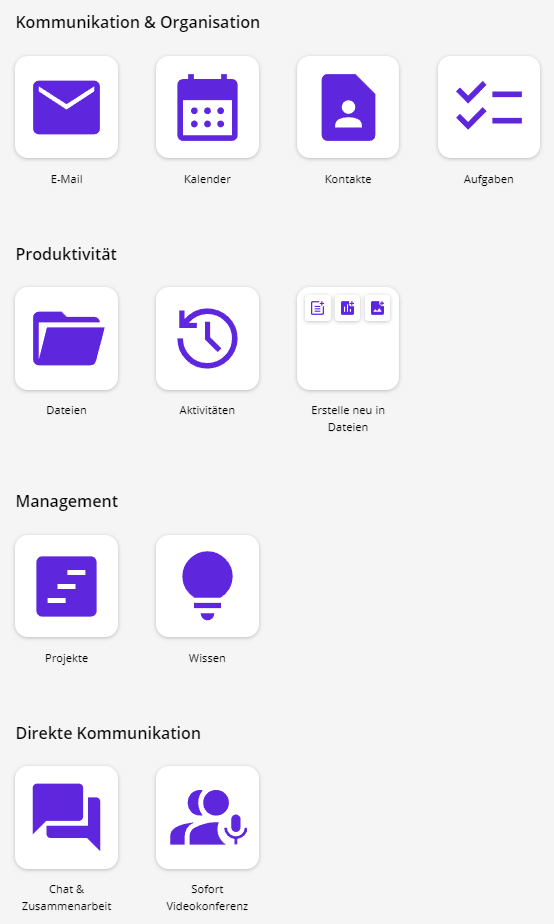
\includegraphics[keepaspectratio]{src/content/docs/user/../../../assets/user/c138d45ee9b60521456074d02500e943fb5bb678.png}}

}

\caption{Portalseite von openDesk}

\end{figure}%

\section{Anwendungen}\label{anwendungen}

Die Dokumentationen der einzelnen Komponenten finden Sie hier:

\begin{longtable}[]{@{}
  >{\raggedright\arraybackslash}p{(\linewidth - 4\tabcolsep) * \real{0.1795}}
  >{\raggedright\arraybackslash}p{(\linewidth - 4\tabcolsep) * \real{0.2372}}
  >{\raggedright\arraybackslash}p{(\linewidth - 4\tabcolsep) * \real{0.5833}}@{}}
\toprule\noalign{}
\begin{minipage}[b]{\linewidth}\raggedright
Anwendungsgruppe
\end{minipage} & \begin{minipage}[b]{\linewidth}\raggedright
Anwendungsname
\end{minipage} & \begin{minipage}[b]{\linewidth}\raggedright
Komponentendokumentation
\end{minipage} \\
\midrule\noalign{}
\endhead
\bottomrule\noalign{}
\endlastfoot
Kommunikation \& Organisation & E-Mail, Kalender, Kontakte \& Aufgaben &
\href{https://www.open-xchange.com/resources/oxpedia}{OX AppSuite} \\
Produktivität & Dateien &
\href{https://docs.nextcloud.com/}{Nextcloud} \\
Produktivität & Diagramme &
\href{https://docs.cryptpad.org/en/}{CryptPad} mit
\href{https://www.diagrams.net/doc/}{diagrams.net} \\
Produktivität & Weboffice &
\href{https://help.collaboraoffice.com/}{Collabora Online} \\
Management & Projekte &
\href{https://www.openproject.org/docs/user-guide/}{OpenProject} \\
Management & Wissen &
\href{https://www.xwiki.org/xwiki/bin/view/Documentation}{XWiki} \\
Direkte Kommunikation & Chat \& Zusammenarbeit &
\href{https://element.io/user-guide}{Element} mit Nordeck widgets \\
Direkte Kommunikation & Sofort Videokonferenz &
\href{https://jitsi.github.io/handbook/docs/category/user-guide/}{Jitsi} \\
Portal & - &
\href{https://docs.software-univention.de/n/en/index.html}{Univention} \\
\end{longtable}

\section{Arbeitsplatz aufrufen}\label{arbeitsplatz-aufrufen}

Ihr Arbeitsplatz wird über einen Internet-Browser (Mozilla Firefox,
Microsoft Edge, Google Chrome oder ein anderer Browser) aufgerufen.
Geben Sie einfach in die Adressleiste Ihre Anmelde-Adresse ein.

\section{Anmeldung}\label{anmeldung}

Zur Anmeldung geben Sie Ihren \textbf{Benutzernamen} oder Ihre
\textbf{E-Mail-Adresse} und das Passwort ein. Nach der
\textbf{Anmeldung} können Sie über das Menü am rechten oberen
Bildschirmrand (drei Balken) die \textbf{Benutzereinstellungen}
verwalten.

\begin{figure}[H]

{\centering \pandocbounded{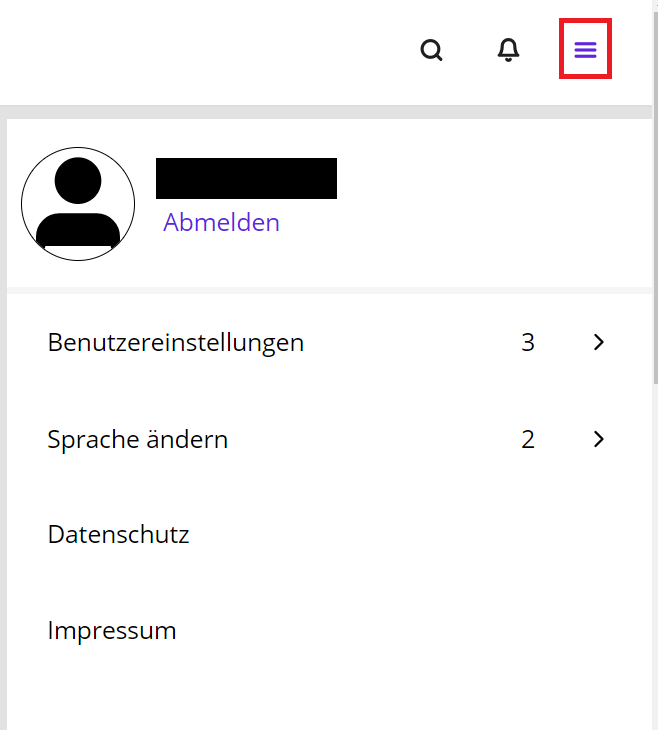
\includegraphics[keepaspectratio]{src/content/docs/user/../../../assets/user/anmeldung.png}}

}

\caption{Anmelden}

\end{figure}%

\section{Abmeldung}\label{abmeldung}

Auf der Startseite Ihres Arbeitsplatzes und in jedem Modul können Sie
sich über das \textbf{Hamburger-Menü} (drei Balken) ganz oben rechts
abmelden.

\begin{figure}[H]

{\centering \pandocbounded{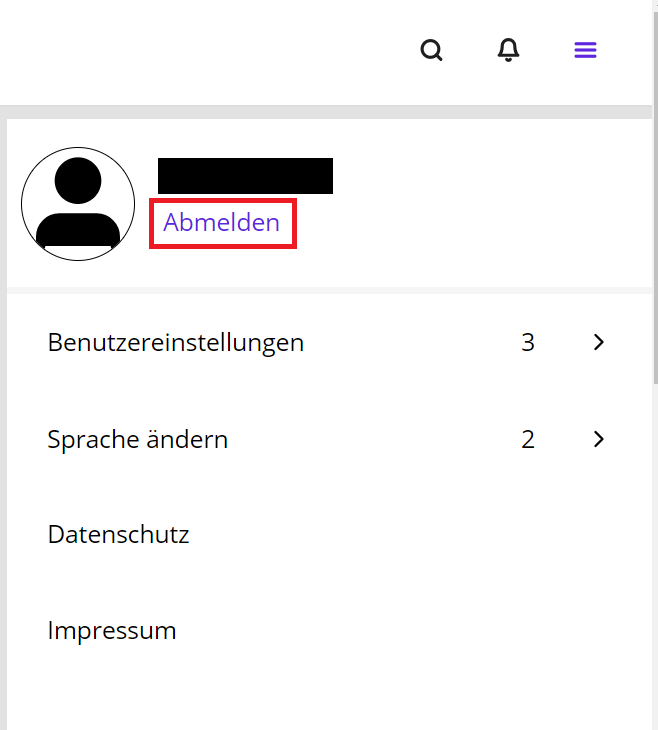
\includegraphics[keepaspectratio]{src/content/docs/user/../../../assets/user/abmeldung.png}}

}

\caption{Abmelden}

\end{figure}%

\chapter{Beteiligung}\label{beteiligung}

Diese Dokumentation ist wie openDesk Open Source. Sie können auf
\href{https://gitlab.opencode.de/bmi/opendesk/documentation/handbooks}{Open
CoDE die Originaldateien} einsehen und sich an der Verbesserung
beteiligen.

\chapter{Kontakte}\label{kontakte}

Mit dem Modul Kontakte haben Sie ein Werkzeug, um verschiedene
Adressbücher zu verwalten. Die darin gespeicherten Adressen können Sie
beim Versenden von E-Mails, bei der Termin- oder Aufgabenplanung und an
vielen weiteren Stellen einsetzen.

\section{Allgemeiner Aufbau des
Moduls}\label{allgemeiner-aufbau-des-moduls}

\begin{enumerate}
\def\labelenumi{\arabic{enumi}.}
\tightlist
\item
  Adressbuch-Werkzeugleiste
\end{enumerate}

\begin{figure}[H]

{\centering \pandocbounded{
\includegraphics[keepaspectratio]{src/content/docs/user/../../../assets/user/caa177aa22838ac390bccd82ff3c8c956177b550.png}}

}

\caption{Werkzeugleiste}

\end{figure}%

\begin{enumerate}
\def\labelenumi{\arabic{enumi}.}
\setcounter{enumi}{1}
\tightlist
\item
  Adressbuch-Ordneransicht
\end{enumerate}

\begin{figure}[H]

{\centering \pandocbounded{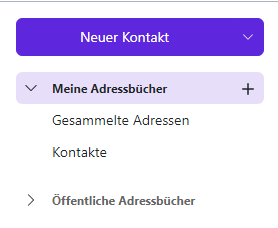
\includegraphics[keepaspectratio]{src/content/docs/user/../../../assets/user/218c0c53bfc2cbaa44ac093e49090596b5b7c4c0.png}}

}

\caption{Adressbuch-Ordneransicht}

\end{figure}%

\begin{enumerate}
\def\labelenumi{\arabic{enumi}.}
\setcounter{enumi}{2}
\tightlist
\item
  Adressbuch-Navigationsbereich
\end{enumerate}

\begin{figure}[H]

{\centering \pandocbounded{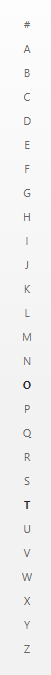
\includegraphics[keepaspectratio]{src/content/docs/user/../../../assets/user/6b1fec9d28abc8f08bfde35b448808a0f41e7f27.png}}

}

\caption{Adressbuch- Navigationsbereich}

\end{figure}%

\begin{enumerate}
\def\labelenumi{\arabic{enumi}.}
\setcounter{enumi}{3}
\tightlist
\item
  Adressbuch-Anzeigebereich
\end{enumerate}

\begin{figure}[H]

{\centering \pandocbounded{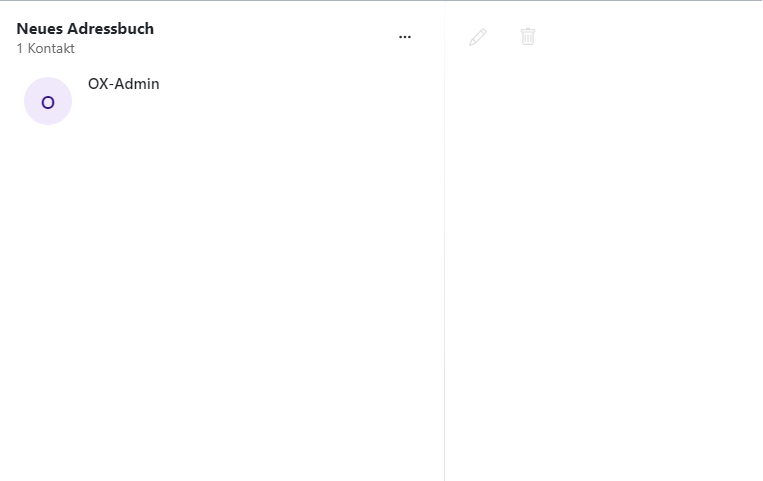
\includegraphics[keepaspectratio]{src/content/docs/user/../../../assets/user/2a9b6b949470613f76661bb6157c91d633796fb9.png}}

}

\caption{Adressbuch-Anzeigebereich}

\end{figure}%

\section{Verteilerliste hinzufügen}\label{verteilerliste-hinzufuxfcgen}

\subsection{Neue Verteilerliste
anlegen}\label{neue-verteilerliste-anlegen}

Öffnen Sie als erstes ein Adressbuch in der Ordneransicht. Klicken Sie
dann in der Werkzeugleiste auf \textbf{Neuer Kontakt} und anschließend
auf \textbf{Neue Verteilerliste}.

\begin{figure}[H]

{\centering \pandocbounded{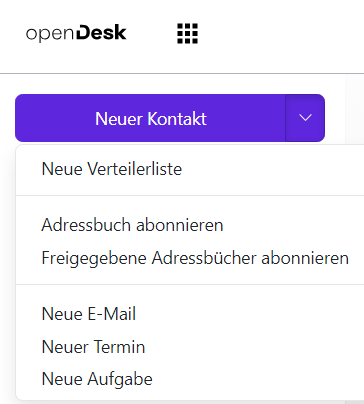
\includegraphics[keepaspectratio]{src/content/docs/user/../../../assets/user/f16d0994b05f33c8466eb1d5b1b38bdeb7124072.png}}

}

\caption{Verteilerliste anlegen}

\end{figure}%

\textbf{Hinweis:} Diese Schritte sind nur in Adressbüchern möglich, in
denen Sie die Berechtigung zum Anlegen von Objekten haben. Das globale
Adressbuch ist hiervon z. B. ausgenommen.

\begin{figure}[H]

{\centering \pandocbounded{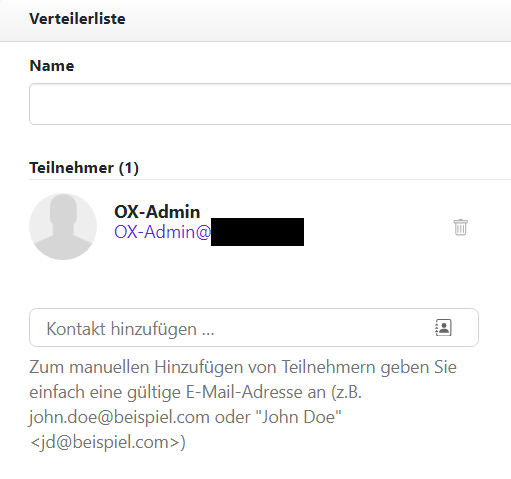
\includegraphics[keepaspectratio]{src/content/docs/user/../../../assets/user/9bcd6835734a510c867311f58fbeba6b79b3fc42.png}}

}

\caption{Verteilerliste anlegen}

\end{figure}%

Geben Sie unter \textbf{Name} einen Namen für die Verteilerliste ein.
Danach geben Sie im Eingabefeld unter der Überschrift
\textbf{Teilnehmer} die E-Mail-Adresse oder den Namen einer Teilnehmerin
oder eines Teilnehmers ein.

\begin{itemize}
\tightlist
\item
  Während der Eingabe werden passende Vorschläge für Sie angezeigt. Um
  einen Vorschlag zu übernehmen, klicken Sie darauf
\end{itemize}

Um Kontakte aus einem Adressbuch zu wählen, klicken Sie rechts im
Eingabefeld auf das Symbol \textbf{Kontakte auswählen} Falls Sie weitere
Kontakte hinzufügen möchten, wiederholen Sie diese letzten Schritte
entsprechend. Möchten Sie einen Kontakt entfernen, klicken Sie neben dem
Kontakt auf das Papierkorb-Symbol.

Klicken Sie abschließend auf \textbf{Liste erstellen}.

\begin{figure}[H]

{\centering \pandocbounded{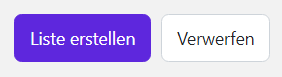
\includegraphics[keepaspectratio]{src/content/docs/user/../../../assets/user/d2a16b8dc7af79e0c63ee25dd352463a370ad696.png}}

}

\caption{Verteilerliste erstellen}

\end{figure}%

\subsection{Kontakte oder Verteilerlisten
bearbeiten}\label{kontakte-oder-verteilerlisten-bearbeiten}

\textbf{Hinweis:} Die folgenden Schritte sind nur in Adressbüchern
möglich, in denen Sie die Berechtigung zum Anlegen von Objekten hast.
Das globale Adressbuch ist hiervon z. B. ausgenommen.

Wählen Sie zuerst in der Liste einen Kontakt oder eine Verteilerliste
aus. Klicken Sie danach in der Werkzeugleiste auf \textbf{Bearbeiten}.

\begin{figure}[H]

{\centering \pandocbounded{
\includegraphics[keepaspectratio]{src/content/docs/user/../../../assets/user/caa177aa22838ac390bccd82ff3c8c956177b550.png}}

}

\caption{Werkzeugleiste Verteilerliste bearbeiten}

\end{figure}%

Es öffnet sich ein Fenster, in dem Sie die Daten des Kontaktes bzw. der
Verteilerliste einsehen und bearbeiten können. Haben Sie alle
gewünschten Änderungen vorgenommen, klicken Sie auf \textbf{Speichern}.

\pandocbounded{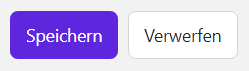
\includegraphics[keepaspectratio]{src/content/docs/user/../../../assets/user/ccf87765da60c04e05b9f5c531d71fc48debf060.png}}

\section{Adressbuch hinzufügen}\label{adressbuch-hinzufuxfcgen}

Mithilfe von Adressbüchern können Sie Ihre Kontakte organisieren, zum
Beispiel unterteilt in berufliche und private Kontakte. Erfahren Sie,
wie Sie Adressbücher anlegen, Kontakte aus externen Adressbüchern
anwenden und die Anzeige von freigegebenen Adressbüchern bestimmen
können.

\subsection{Persönliches Adressbuch
hinzufügen}\label{persuxf6nliches-adressbuch-hinzufuxfcgen}

Unter \textbf{Meine Adressbücher} können Sie persönliche Adressbücher
anlegen. Um ein neues Adressbuch anzulegen, klicken Sie auf das
\textbf{Plus (+)} neben \textbf{Meine Adressbücher.}

\begin{figure}[H]

{\centering \pandocbounded{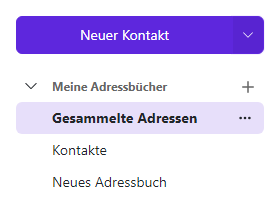
\includegraphics[keepaspectratio]{src/content/docs/user/../../../assets/user/d1ab51e40e4e106027be2dc3175a112f55455ca1.png}}

}

\caption{Adressbuch anlegen}

\end{figure}%

Wählen Sie jetzt das \textbf{Plus (+)} , um ein neues Adressbuch zu
erstellen.

\begin{figure}[H]

{\centering \pandocbounded{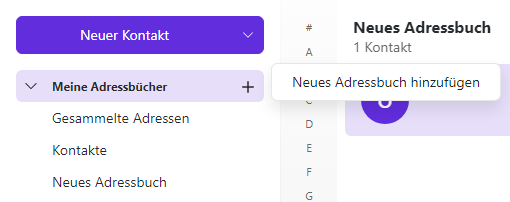
\includegraphics[keepaspectratio]{src/content/docs/user/../../../assets/user/9512f959675708ad4d05e1484718f4cf69deae3c.png}}

}

\caption{Neues Adressbuch hinzufügen}

\end{figure}%

Es erscheint ein neues Fenster, in dem Sie Ihr neues Adressbuch benennen
können. Soll das Adressbuch öffentlich einsehbar sein, setzen Sie den
Haken bei \textbf{Als öffentlichen Ordner hinzufügen.} Klicken Sie
abschließend auf \textbf{Hinzufügen}.

\begin{figure}[H]

{\centering \pandocbounded{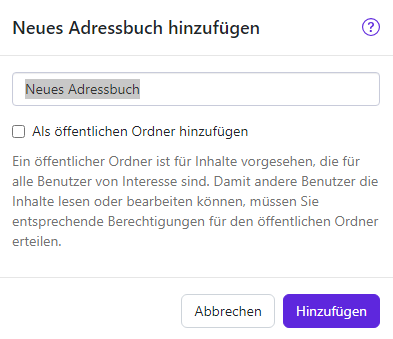
\includegraphics[keepaspectratio]{src/content/docs/user/../../../assets/user/e69b72344b7f0e11154514a25cbcf3c632632d4b.png}}

}

\caption{Neues Adressbuch hinzufügen}

\end{figure}%

\subsection{Öffentliche
Adressbücher}\label{uxf6ffentliche-adressbuxfccher}

Sie können innerhalb des Moduls \textbf{Kontakte} öffentliche
Adressbücher einsehen, welche in der Seitenansicht untereinander
aufgelistet sind.

\begin{figure}[H]

{\centering \pandocbounded{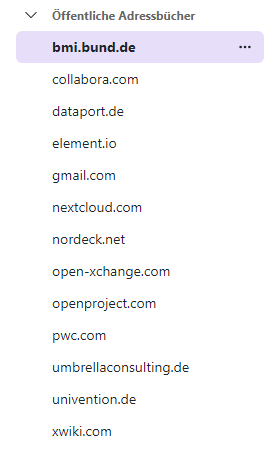
\includegraphics[keepaspectratio]{src/content/docs/user/../../../assets/user/9de3b5c229a61ac70c95e976a1adfd873717a218.png}}

}

\caption{Öffentliche Adressbücher Auflistung}

\end{figure}%

Sie haben die Möglichkeit öffentliche Adressbücher zu Ihren Favoriten
hinzuzufügen, Ihre Berechtigungen für dieses Adressbuch einzusehen, das
Adressbuch zu exportieren und es auszublenden. Klicken Sie dafür auf das
Dreipunkt-Menü neben dem entsprechenden Adressbuch und klicken Sie auf
die gewünschte Funktion.

\begin{figure}[H]

{\centering \pandocbounded{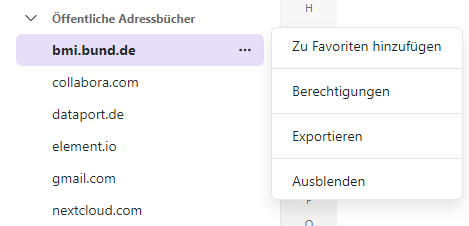
\includegraphics[keepaspectratio]{src/content/docs/user/../../../assets/user/6c5bdcbf943ec0d1a53b9d9f092372d6fa2fe9d2.png}}

}

\caption{Öffentliche Adressbücher Funktionen}

\end{figure}%

\section{Neuen Kontakt hinzufügen}\label{neuen-kontakt-hinzufuxfcgen}

Das Modul Kontakte ermöglicht die Verwaltung aller Adressbücher und
persönlichen Kontakte.

Das Anlegen neuer und das Bearbeiten vorhandener Kontakte und Adressen
erfolgt über die Menüleiste.

Über den Menüpunkt \textbf{Neuer Kontakt} besteht auch die Möglichkeit,
Verteilerlisten zu erstellen.

Wenn Sie einen neuen Kontakt hinzufügen möchten, navigieren Sie links zu
\textbf{Meine Adressbücher} und wählen Sie ein Adressbuch aus. Klicken
Sie nun auf die violette Schaltfläche \textbf{Neuer Kontakt}.
Anschließend öffnet sich ein neues Fenster. Jetzt haben Sie die
Möglichkeit, die gewünschten Kontaktdaten einzugeben.

\begin{figure}[H]

{\centering \pandocbounded{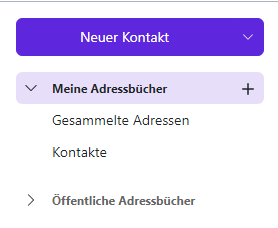
\includegraphics[keepaspectratio]{src/content/docs/user/../../../assets/user/0c9b1b6ed2b10d7c9a9830c5c56c55124be30b57.png}}

}

\caption{Neuen Kontakt hinzufügen}

\end{figure}%%
\begin{figure}[H]

{\centering \pandocbounded{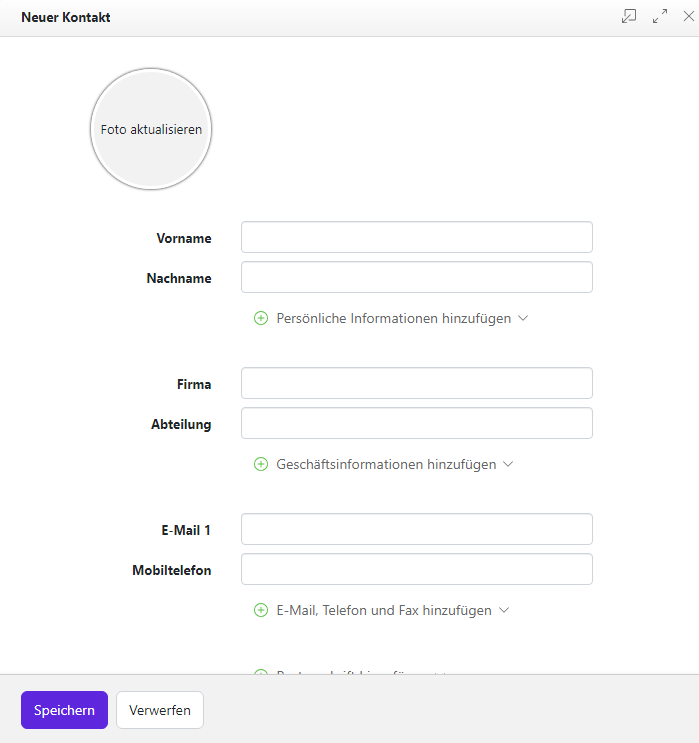
\includegraphics[keepaspectratio]{src/content/docs/user/../../../assets/user/858e974efefd79d63f9f87a7e44888b981db3eb3.png}}

}

\caption{Kontaktdaten eingeben}

\end{figure}%

Wenn Sie einem Kontakt ein Foto hinzufügen möchten, klicken Sie auf das
leere Kontaktfoto. Das Fenster \textbf{Kontaktfoto ändern} öffnet sich.
Wenn Sie ein vorhandenes Foto hochladen möchten, klicken Sie auf
\textbf{Ein Foto hochladen.} Möchten Sie direkt ein neues Foto mithilfe
der Gerätekamera aufnehmen, klicken Sie auf \textbf{Ein Foto machen}.
Bei Bedarf können Sie den Bildausschnitt festlegen, indem Sie den Regler
unter dem Foto verwenden und das Foto verschieben oder drehen.

Wenn Sie auf \textbf{Anwenden} klicken, wird das Foto hinzugefügt.

\begin{figure}[H]

{\centering \pandocbounded{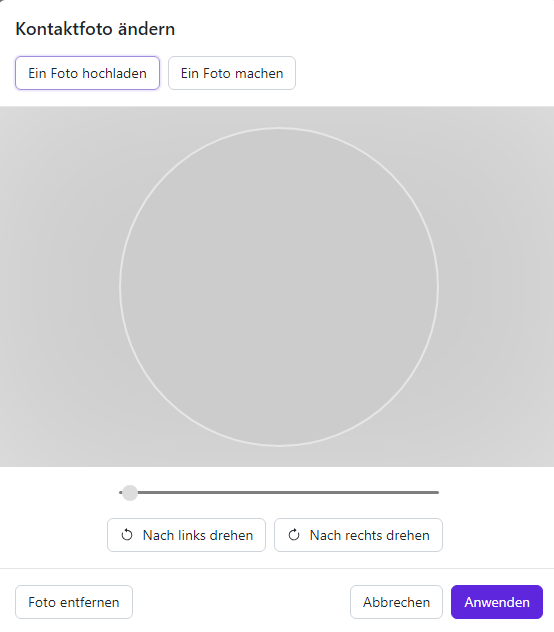
\includegraphics[keepaspectratio]{src/content/docs/user/../../../assets/user/3a3a43dbc9e8f1d6a554ff48c7a630d256a94b3b.png}}

}

\caption{Kontaktfoto ändern}

\end{figure}%

Um ein Foto zu bearbeiten oder zu löschen, klicken Sie zunächst auf das
Foto. Damit gelangen Sie in eine Editor-Ansicht, in der Sie das Bild
über die entsprechenden Schaltflächen drehen können. Verwenden Sie den
horizontalen Regler, um die Zoomstufe zu verändern. Wenn Sie näher an
das Bild herangezoomt haben, können Sie im Folgenden den Bildausschnitt
verändern, indem Sie auf das Bild klicken und es mit gedrückter
Maustaste verschieben. Klicken Sie auf \textbf{Anwenden}, sobald Sie mit
Ihren Änderungen zufrieden sind, oder wählen Sie \textbf{Foto entfernen}
, wenn das Bild ganz gelöscht werden soll.

\begin{figure}[H]

{\centering \pandocbounded{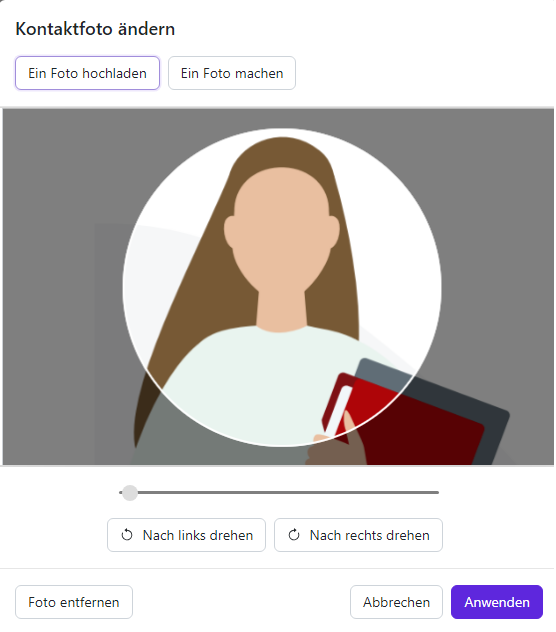
\includegraphics[keepaspectratio]{src/content/docs/user/../../../assets/user/8fe9d7fa5a6300c1caeb752079522a954f97013e.png}}

}

\caption{Kontaktfoto bearbeiten}

\end{figure}%%
\begin{figure}[H]

{\centering \pandocbounded{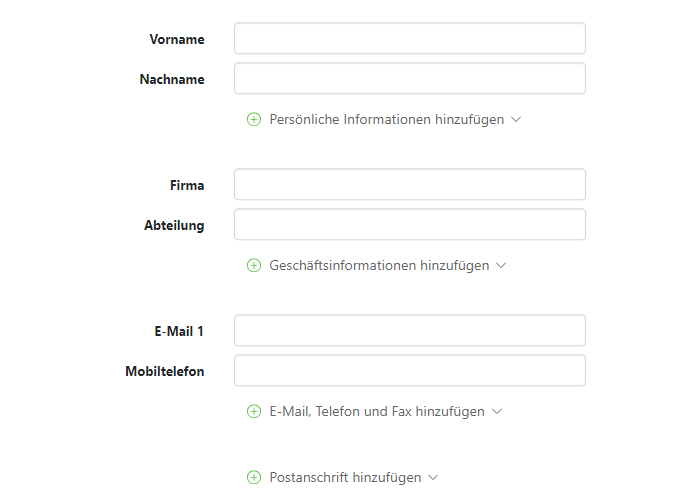
\includegraphics[keepaspectratio]{src/content/docs/user/../../../assets/user/b2c01466192b8ff4502aa49b0559b64133c0ed1f.png}}

}

\caption{Kontaktdaten eingeben}

\end{figure}%%
\begin{figure}[H]

{\centering \pandocbounded{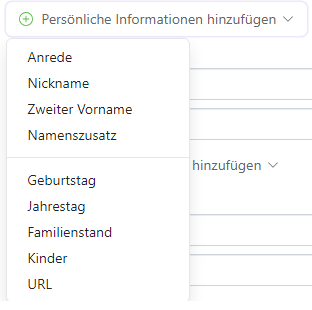
\includegraphics[keepaspectratio]{src/content/docs/user/../../../assets/user/9a51b2d41a9401e74bb851de62c7a5133d1d6a70.png}}

}

\caption{Persönliche Informationen hinzufügen}

\end{figure}%

Der Firma bzw. der Abteilung können auch weitere Informationen
hinzugefügt werden. Klicken Sie dafür auf \textbf{Geschäftsinformationen
hinzufügen}. Es erscheint ein Dropdown-Menü und Sie können die
Informationen um weitere Punkte ergänzen:

\begin{itemize}
\tightlist
\item
  \textbf{Position}
\item
  \textbf{Beruf}
\item
  \textbf{Raumnummer}
\item
  \textbf{Manager}
\item
  \textbf{Assistent}
\end{itemize}

\begin{figure}[H]

{\centering \pandocbounded{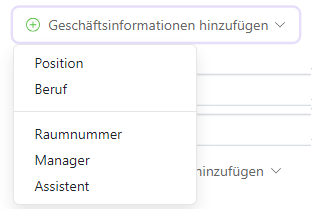
\includegraphics[keepaspectratio]{src/content/docs/user/../../../assets/user/3bbc9da118d5e56bd3c6e9939a0b1bf673b6d1ef.png}}

}

\caption{Geschäftsinformationen hinzufügen}

\end{figure}%

Sollten Sie mehrer E-Mail-Adressen besitzen, können Sie diese ebenfalls
hinzufügen. Klicken Sie dafür auf \textbf{E-Mail, Telefon, Fax
hinzufügen}. Es erscheint ein Dropdown-Menü und Sie können die
Informationen um weitere Punkte ergänzen:

\begin{itemize}
\tightlist
\item
  \textbf{E-Mail 2}
\item
  \textbf{E-Mail 3}
\item
  \textbf{Instantmessenger 1}
\item
  \textbf{Instantmessenger 2}
\item
  \textbf{Mobiltelefon (2)}
\item
  \textbf{Telefon (geschäftlich)}
\item
  \textbf{Telefon (geschäftlich 2)}
\item
  \textbf{Telefon (privat)}
\item
  \textbf{Telefon (privat 2)}
\item
  \textbf{Telefon (Zentrale)}
\item
  \textbf{Telefon (weiteres)}
\item
  \textbf{Fax}
\item
  \textbf{Fax (privat)}
\item
  \textbf{Fax(2)}
\end{itemize}

\begin{figure}[H]

{\centering \pandocbounded{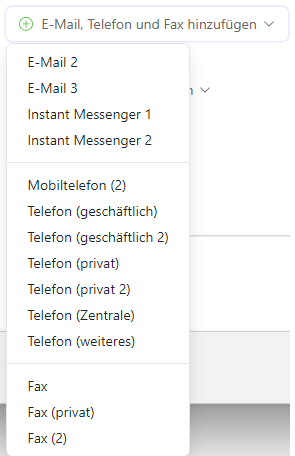
\includegraphics[keepaspectratio]{src/content/docs/user/../../../assets/user/0b406ab1528f7e695f5a60bb3f7192c70a652b55.png}}

}

\caption{E-Mail, Telefon, Fax hinzufügen}

\end{figure}%

Darüber hinaus haben Sie die Option eine Kategorie Ihres Termins
anzugeben, welche Ihnen erscheint, wenn Sie auf den rechten Pfeil neben
\textbf{Kategorie hinzufügen} klicken. Die Kategorien sind
voreingestellt und es kann \textbf{Predefined}, \textbf{Important},
\textbf{Business}, \textbf{Private} und \textbf{Meeting} ausgewählt
werden. Möchten Sie nützliche Notizen hinzufügen können Sie im Textfeld
Notiz Ihre Angaben machen. Sollte dieser Kontakt als privater Kontakt
eingestuft werden, können Sie die Checkbox \textbf{Dies ist ein privater
Kontakt und kann nicht freigegeben werden} anklicken. Außerdem haben Sie
die Möglichkeit Benutzerfelder hinzuzufügen. Das können Sie einstellen,
indem Sie auf \textbf{Benutzerfelder hinzufügen} klicken. Um dem Termin
Anhänge hinzuzufügen, klicken Sie entweder auf \textbf{Anhänge
hinzufügen} oder \textbf{Von Dateien hinzufügen.}

\begin{figure}[H]

{\centering \pandocbounded{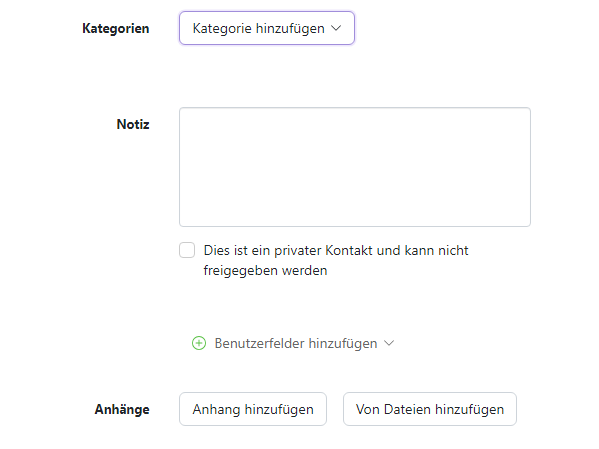
\includegraphics[keepaspectratio]{src/content/docs/user/../../../assets/user/620783f92c4a3db370178ba646d58e7c49c90aea.png}}

}

\caption{Kategorie, Notizen, Anhänge hinzufügen}

\end{figure}%

\section{Kontakt löschen}\label{kontakt-luxf6schen}

Möchten Sie einen bereits bestehenden Kontakt löschen, müssen Sie
zunächst den gewünschten Kontakt auswählen, sodass dieser violett
hinterlegt ist. Anschließend wählen Sie in der oberen Leiste das Icon
\textbf{Löschen} aus.

\begin{figure}[H]

{\centering \pandocbounded{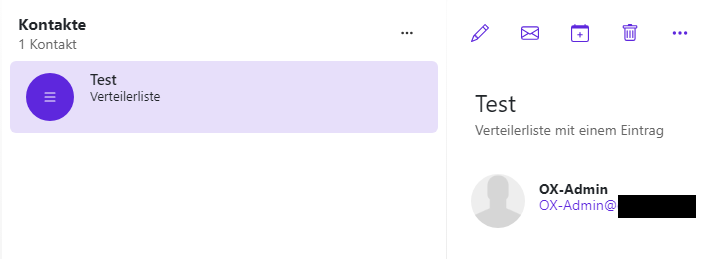
\includegraphics[keepaspectratio]{src/content/docs/user/../../../assets/user/8481991695cd7697aa47e69c4eb7052ac970a36d.png}}

}

\caption{Kontakt löschen}

\end{figure}%

Anschließend werden Sie gefragt, ob der Kontakt wirklich gelöschen
werden soll. Wenn Sie dies tun möchten, klicken Sie auf
\textbf{Löschen}.

\begin{figure}[H]

{\centering \pandocbounded{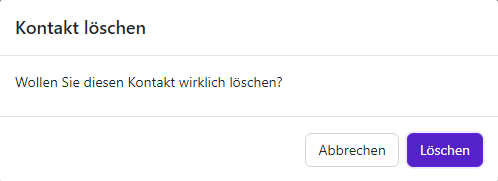
\includegraphics[keepaspectratio]{src/content/docs/user/../../../assets/user/1e0d2477699e927509115b18ab47edfcb53f38f7.png}}

}

\caption{Kontakt löschen}

\end{figure}%

\section{Kontakt verschieben oder
kopieren}\label{kontakt-verschieben-oder-kopieren}

Sie können Kontakte oder Verteilerlisten in ein anderes Adressbuch
verschieben oder kopieren. Das globale Adressbuch ist hiervon allerdings
ausgenommen.

So verschieben oder kopieren Sie Kontakte in ein anderes Adressbuch:

Wählen Sie in der Liste einen oder mehrere Kontakte oder Verteilerlisten
aus, welche Sie kopieren oder verschieben möchten. Klicken Sie
anschließend in der Werkzeugleiste auf das Symbol \textbf{Weitere
Aktionen (Hamburger-Menü)} . Danach können Sie auf \textbf{Verschieben}
oder \textbf{Kopieren} klicken. Jetzt öffnet sich ein Fenster, in
welchem Sie ein Adressbuch auswählen. Bei Bedarf können Sie auch ein
neues Adressbuch anlegen, indem Sie auf \textbf{Ordner anlegen} klicken.
Klicken Sie nun auf \textbf{Verschieben} beziehungsweise
\textbf{Kopieren}.

\textbf{Tipp:} Sie können die gewählten Kontakte bzw. Verteilerlisten
auch per Drag \& Drop verschieben, indem Sie diese in der Ordneransicht
einfach mit gedrückter Maustaste auf ein Adressbuch ziehen.

\begin{figure}[H]

{\centering \pandocbounded{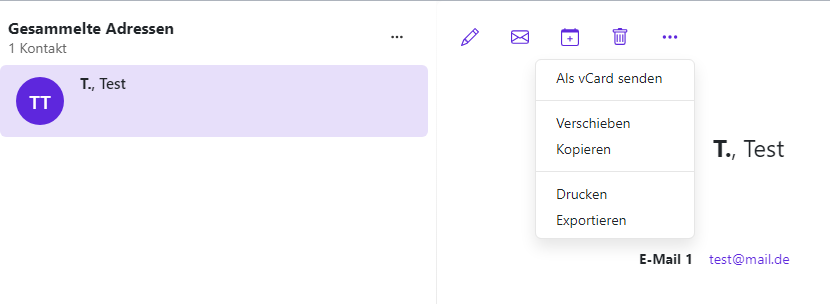
\includegraphics[keepaspectratio]{src/content/docs/user/../../../assets/user/04f1c0996d180f08bb34e8cad7c778deec299d9d.png}}

}

\caption{Kontakt verschieben oder kopieren}

\end{figure}%%
\begin{figure}[H]

{\centering \pandocbounded{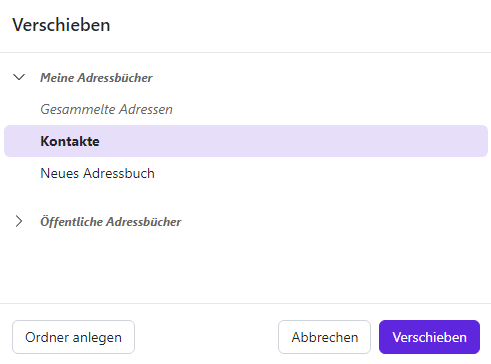
\includegraphics[keepaspectratio]{src/content/docs/user/../../../assets/user/66d38ab4439ebde2e5d70ea78e72e70e86c02e50.png}}

}

\caption{Kontakt verschieben}

\end{figure}%

\section{Kontakt als vCard versenden}\label{kontakt-als-vcard-versenden}

So können Sie Kontakte oder Verteilerlisten als vCard-Anhang in einer
E-Mail versenden:

Zu Beginn wählen Sie in der Liste einen Kontakt, eine Verteilerliste
oder mehrere Kontakte oder Verteilerlisten aus. Anschließend klicken Sie
in der Werkzeugleiste auf das Symbol \textbf{Weitere Aktionen
(Hamburger-Menü).} Wenn sie jetzt auf auf \textbf{Als vCard senden
klicken} , wird eine vCard versendet.

\begin{figure}[H]

{\centering \pandocbounded{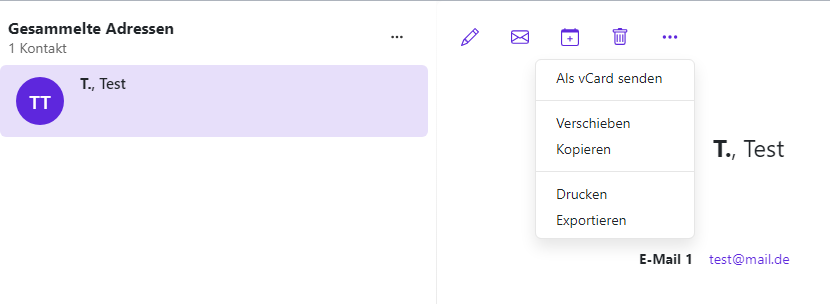
\includegraphics[keepaspectratio]{src/content/docs/user/../../../assets/user/04f1c0996d180f08bb34e8cad7c778deec299d9d.png}}

}

\caption{Kontakt als vCard versenden}

\end{figure}%

Anschließend können Sie die Angaben der E-Mail vervollständigen. Wie in
einer regulären E-Mail können Sie folgende Daten eingeben:

\begin{itemize}
\tightlist
\item
  E-Mail-Adresse, an die der Kontakt versendet werden soll
\item
  Betreff
\item
  Text der E-Mail
\item
  Anhänge
\end{itemize}

Um die E-Mail mit der vCard abzusenden, klicken Sie auf \textbf{Senden}.

\begin{figure}[H]

{\centering \pandocbounded{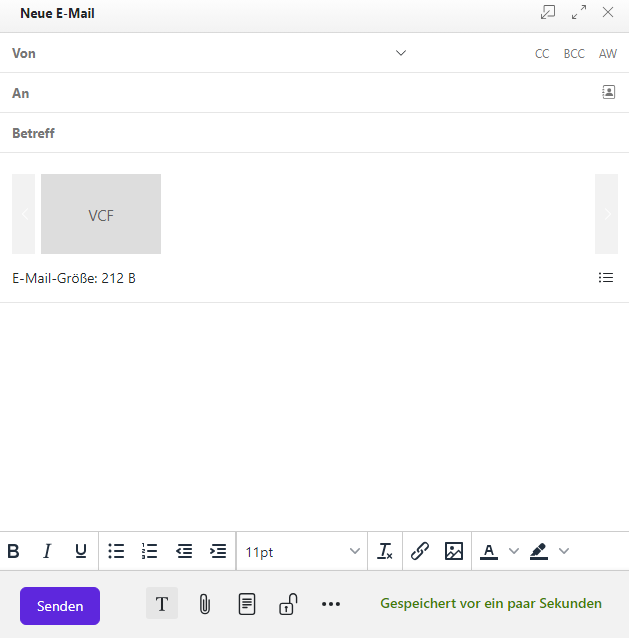
\includegraphics[keepaspectratio]{src/content/docs/user/../../../assets/user/f18a2ece38d71155c01fe2f473a55f969e1936a2.png}}

}

\caption{vCard versenden}

\end{figure}%

\section{Kontakt zu einem Termin
einladen}\label{kontakt-zu-einem-termin-einladen}

Sie können direkt aus dem Modul \textbf{Kontakte} Termine anlegen und
Kontakte oder ganze Verteilerlisten zu diesen Terminen einladen. Wählen
Sie zu Beginn einen oder mehrere Kontakte oder Verteilerlisten aus und
klicken Sie anschließend in der Werkzeugleiste auf \textbf{Zu Termin
Einladen}. Wenn Sie einen einzelnen Kontakt auswählen möchten, klicken
Sie alternativ oben in der Detailansicht des Kontaktes auf
\textbf{Einladen}. Als letzten Schritt können Sie die Angaben zum
Anlegen des Termins vervollständigen. Nähere Angaben hierzu finden Sie
unter
\href{../../kalender/termin-einstellen/termin-einstellen.md}{Termin
einstellen}.

\begin{figure}[H]

{\centering \pandocbounded{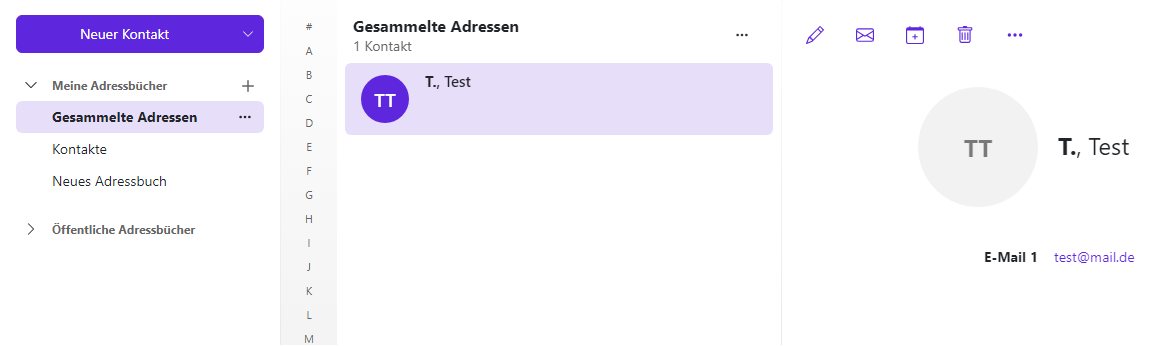
\includegraphics[keepaspectratio]{src/content/docs/user/../../../assets/user/b57726f793631e8cbbb446bf291b8103a579f82d.png}}

}

\caption{Kontakt zu einem Termin einladen}

\end{figure}%%
\begin{figure}[H]

{\centering \pandocbounded{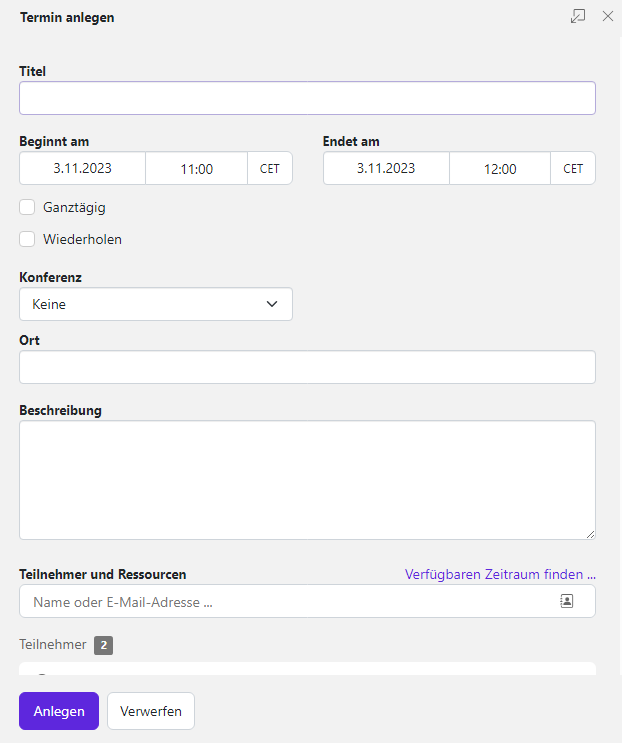
\includegraphics[keepaspectratio]{src/content/docs/user/../../../assets/user/a53d86bc88ecf016f2be84d0775f28fccac27767.png}}

}

\caption{Termin anlegen}

\end{figure}%

\section{Neuen Termin anlegen}\label{neuen-termin-anlegen}

So können Sie einen neuen Termin anlegen:

Zuerst öffnen Sie in der Ordneransicht einen Kalender, in dem Sie die
Berechtigung zum Anlegen von Objekten haben. Danach klicken Sie in der
Werkzeugleiste auf \textbf{Einladen}.

\begin{figure}[H]

{\centering \pandocbounded{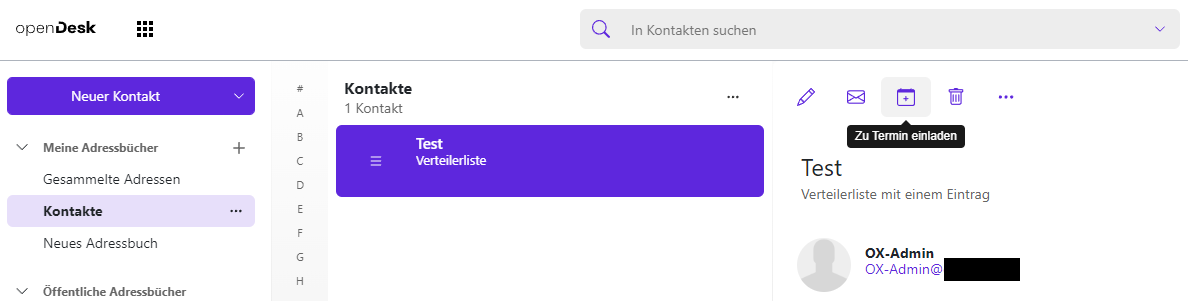
\includegraphics[keepaspectratio]{src/content/docs/user/../../../assets/user/4b8de26ed7fc39cefafe0a37e97d34ba94aed3e7.png}}

}

\caption{Zu einem Termin einladen}

\end{figure}%

Zuerst müssen Sie einen \textbf{Titel} eingeben.

\begin{figure}[H]

{\centering \pandocbounded{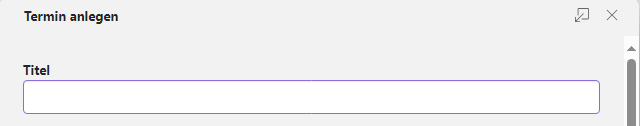
\includegraphics[keepaspectratio]{src/content/docs/user/../../../assets/user/c3c074f213189c8717c5a129058fa94300676395.png}}

}

\caption{Neuen Termin anlegen, Titel festlegen}

\end{figure}%

Um den Beginn und das Ende des Termins festzulegen, müssen Sie unterhalb
von \textbf{Beginnt am} und \textbf{Endet am} folgenden Aktionen
ausführen:

\begin{itemize}
\tightlist
\item
  Klicken Sie auf ein Datum. Geben Sie ein Datum ein oder wählen Sie ein
  Datum aus der Datumsauswahl. Bei ganztägigen Terminen aktivierst du
  \textbf{Ganztägig}
\item
  Klicken Sie auf eine Uhrzeit. Geben Sie die Uhrzeit ein, oder wählen
  Sie eine Uhrzeit aus der Liste
\item
  Wenn gewünscht, können Sie die Zeitzone für die Start- oder Endzeit
  festlegen, indem Sie neben einer Uhrzeit auf die
  Zeitzonen-Schaltfläche klicken. Sie können für die Startzeit und
  Endzeit unterschiedliche Zeitzonen angeben
\end{itemize}

\pandocbounded{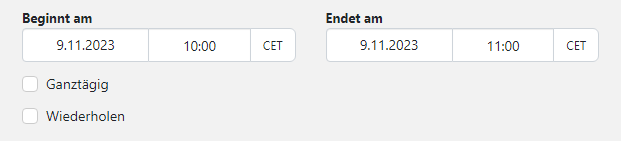
\includegraphics[keepaspectratio]{src/content/docs/user/../../../assets/user/0fa0bea2547a7fa7e8d5ab0125760928c5543743.png}}
- Aktivieren Sie \textbf{Wiederholen}, wenn sich der Termin periodisch
wiederholen soll. Nun erscheint der aktuelle Wochentag in violetter
Schrift. Möchten Sie die Wiederholungszeit verändern, klicken Sie auf
den violetten Wochentag. Es öffnet sich ein neues Fenster. Hier können
nun die terminlichen Aspekte des Termins bearbeitet werden. Haben Sie
Ihre gewünschten Änderungen vorgenommen, klicken Sie auf
\textbf{Anwenden}.

\begin{figure}[H]

{\centering \pandocbounded{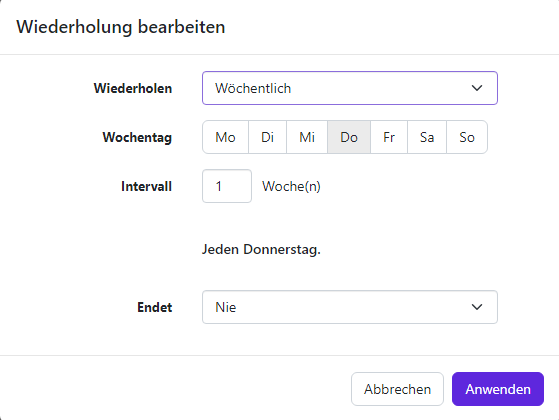
\includegraphics[keepaspectratio]{src/content/docs/user/../../../assets/user/752246ddbac3d55756bb09a34dbbd16bf59c6570.png}}

}

\caption{Termin anlegen, Wiederholung bearbeiten}

\end{figure}%

Möchten Sie den Termin in einer Videokonferenz abhalten, so wählen Sie
unter \textbf{Konferenz} die Möglichkeit \textbf{Videokonferenz} aus.
Das System erstellt einen Konferenzraum und generiert den dazugehörigen
Link automatisch.

\begin{figure}[H]

{\centering \pandocbounded{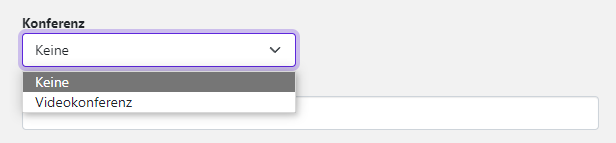
\includegraphics[keepaspectratio]{src/content/docs/user/../../../assets/user/a7523b815151e29fb5eac8f69e29d6c9ac9a250b.png}}

}

\caption{Termin anlegen, Videokonferenz auswählen}

\end{figure}%

Geben Sie bei Bedarf nun den \textbf{Ort} und eine \textbf{Beschreibung}
ein.

Unter \textbf{Teilnehmer} haben Sie die Option, weitere Teilnehmerinnen
und Teilnehmer für den Termin einzuladen. Außerdem haben sehen Sie unter
\textbf{Teilnehmer} , welche Teilnehmerinnen und Teilnehmer sich bereits
in dem Termin befinden. Um weitere Teilnehmerinnen und Teilnehmer in
diesen Termin einzuladen, klicken Sie dafür neben dem Feld
\textbf{Teilnehmer und Ressourcen} auf das Symbol \textbf{Kontakt
auswählen}.

\begin{figure}[H]

{\centering \pandocbounded{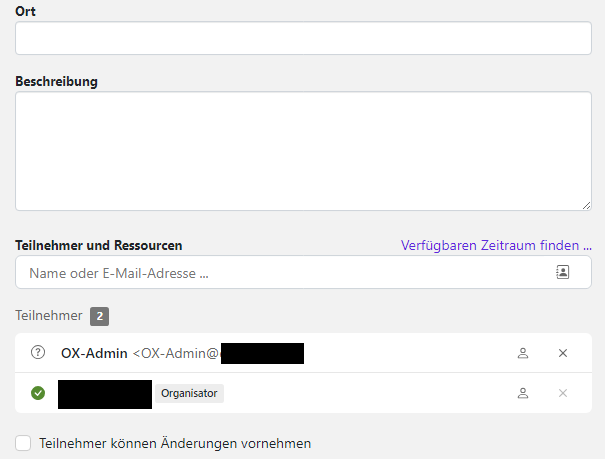
\includegraphics[keepaspectratio]{src/content/docs/user/../../../assets/user/faa44b97d4e0a575ed77af6775df646f08ca046a.png}}

}

\caption{Termin anlegen, Ort, Beschreibung, Teilnehmerinnen und
Teilnehmer einladen}

\end{figure}%

Nun öffnet sich ein neues Fenster mit Ihren Kontakten. Möchten Sie
Kontakte hinzufügen, tippen Sie in das Eingabefeld \textbf{Suchen} den
entsprechenden Namen des Kontakts ein und wählen ihn anschließend aus.
Die ausgewählten Kontakte haben nun einen grauen Hintergrund. Klicke auf
\textbf{Wählen} um deine gewünschten Kontakte zu dem Termin
hinzuzufügen. Sie haben außerdem die Möglichkeit Kontakte zu filtern und
in Ihren verschiedenen Adressbüchern nach Kontakten zu suchen. Die
Schaltflächen befinden sich jeweils rechts neben dem Eingabefeld
\textbf{Suchen}.

\begin{figure}[H]

{\centering \pandocbounded{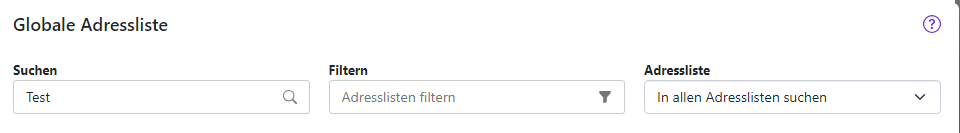
\includegraphics[keepaspectratio]{src/content/docs/user/../../../assets/user/210167904fea7e4d14104273f77f8b0db392a3b1.png}}

}

\caption{Globale Adressliste, Suchen, Filtern, Adressliste}

\end{figure}%

Wenn Sie die Sichtbarkeit Ihres Termins einstellen möchten, können Sie
unter \textbf{Sichtbarkeit} auf den rechten Pfeil in der Schaltfläche
klicken und \textbf{Standard}, \textbf{Privat} oder \textbf{Geheim}
auswählen. Sie können außerdem eine \textbf{Erinnerung} für den Termin
angeben, sodass die entsprechende Teilnehmerin bzw. der entsprechende
Teilnehmer an den Termin erinnert wird. Sie können den gewünschten
Kalender auswählen, in dem der Termin erscheinen soll und sie können die
\textbf{Terminfarbe} auswählen, in der der Termin angezeigt werden soll.
Darüber hinaus haben Sie die Option eine Kategorie Ihres Termins
anzugeben, welche Ihnen erscheint, wenn Sie auf den rechten Pfeil neben
\textbf{Kategorie hinzufügen} klicken. Die Kategorien sind
voreingestellt und es kann \textbf{Predefined}, \textbf{Important},
\textbf{Business}, \textbf{Private} und \textbf{Meeting} ausgewählt
werden. Um dem Termin Anhänge hinzuzufügen, klicken Sie entweder auf
\textbf{Anhänge hinzufügen} oder \textbf{Von Dateien hinzufügen.}

\begin{figure}[H]

{\centering \pandocbounded{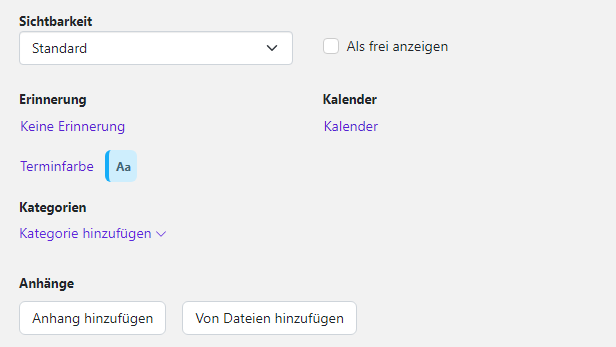
\includegraphics[keepaspectratio]{src/content/docs/user/../../../assets/user/e06e3c18927a25b8337c68829d9e054d963b8caa.png}}

}

\caption{Termin anlegen, weitere Funktionen}

\end{figure}%

Haben Sie nun Ihren Termin fertig konfiguriert, müssen Sie ihn noch
speichern.Sie speichern den Termin, indem Sie auf \textbf{Anlegen}
klicken.

\begin{figure}[H]

{\centering \pandocbounded{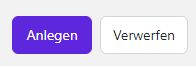
\includegraphics[keepaspectratio]{src/content/docs/user/../../../assets/user/eec945390db2dadcddff544789b3e1e658e88067.png}}

}

\caption{Termin anlegen}

\end{figure}%

\chapter{Kalender}\label{kalender}

Nach Auswählen des Moduls Kalender öffnet sich die Kalenderansicht des
aktuellen Monats. Einmal ist für Sie großflächig die aktuelle
Kalenderwoche angezeigt. Im Minikalender links daneben haben Sie
außerdem eine Darstellung des aktuellen Monats. So haben Sie direkt
einen Überblick über anstehende Termine.

\section{Kalender freigeben}\label{kalender-freigeben}

Sie können Ihren eigenen Kalender für andere Personen freigeben. Öffnen
Sie das Hamburger-Menü neben dem freizugebenden Kalender und klicken Sie
dann bei den angezeigten Optionen auf \textbf{Freigeben/Berechtigungen}.

\begin{figure}[H]

{\centering \pandocbounded{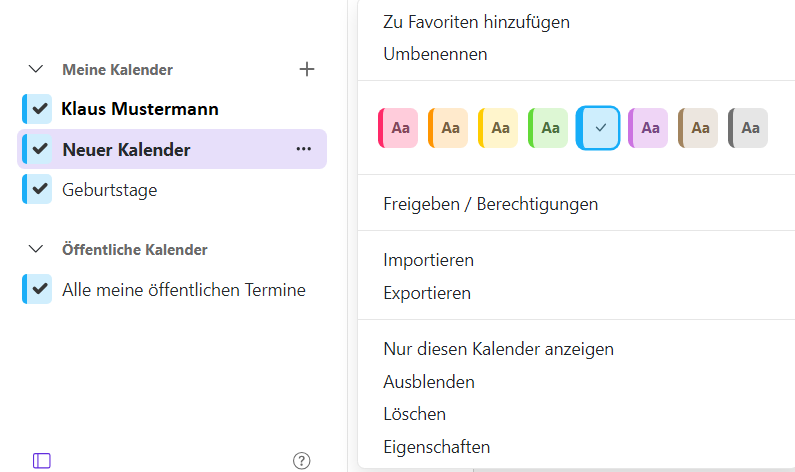
\includegraphics[keepaspectratio]{src/content/docs/user/../../../assets/user/f50102c564d96aa9ce8eca553edf6a6401b30714.png}}

}

\caption{Kalender freigeben}

\end{figure}%

Nun können Sie bestimmen, wer auf den Kalender zugreifen kann. Sie
können Personen einladen und spezifische Rechte für den Kalenderzugriff
festlegen.

\begin{figure}[H]

{\centering \pandocbounded{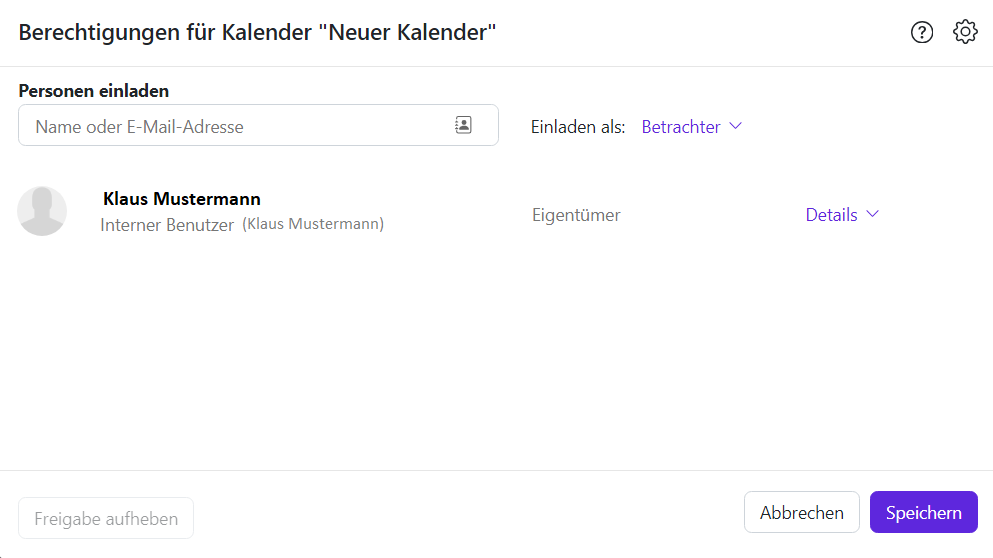
\includegraphics[keepaspectratio]{src/content/docs/user/../../../assets/user/943d5070d723d8f4f8a55f3175e7588f1dbcacd7.png}}

}

\caption{Berechtigung für ausgewählten Kalender}

\end{figure}%

\section{Kalender hinzufügen}\label{kalender-hinzufuxfcgen}

\subsection{Kalender hinzufügen}\label{kalender-hinzufuxfcgen-1}

Sie können beliebig viele Kalender erstellen, zum Beispiel für
unterschiedliche Projekte. Sie können diese auch flexibel öffnen.

Einen neuen Kalender erstellen Sie über den Punkt \textbf{Neuen Kalender
hinzufügen}. Hier können Sie entscheiden, ob es ein persönlicher
Kalender oder ein Kalender für andere Zwecke werden soll. Wenn das der
Fall ist, können Sie auf \textbf{Neuen Ressourcenkalender hinzufügen}
oder \textbf{Neue Ressourcenkalendergruppe hinzufügen} klicken.

\begin{figure}[H]

{\centering \pandocbounded{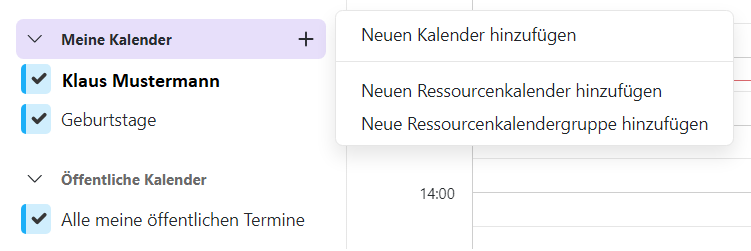
\includegraphics[keepaspectratio]{src/content/docs/user/../../../assets/user/28d50266f65f5cdcb9ede6f73a7699e9ab6b9f44.png}}

}

\caption{Kalender hinzufügen}

\end{figure}%

\subsection{Persönlichen Kalender
hinzufügen}\label{persuxf6nlichen-kalender-hinzufuxfcgen}

Möchten Sie einen persönlichen Kalender erstellen, wählen Sie
\textbf{Neuen Kalender hinzufügen} aus. Ein neues Fenster öffnet sich
und Sie können den neuen Kalender benennen. In diesem Fenster besteht
ebenfalls die Möglichkeit, Ihren persönlichen Kalender in einen
öffentlichen Kalender umzuwandeln. Dieses Feld wird also leer gelassen,
wenn Sie den Kalender nur für sich selbst erstellen möchten. Durch einen
Klick auf \textbf{Hinzufügen} wird der neue Kalender erstellt und in
Ihre Liste aller Kalender mit aufgenommen.

\begin{figure}[H]

{\centering \pandocbounded{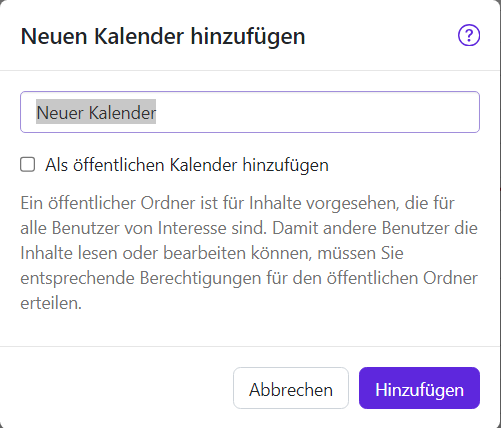
\includegraphics[keepaspectratio]{src/content/docs/user/../../../assets/user/683051ed53d093ba816ebca09870c165c75d9e46.png}}

}

\caption{Persönlichen Kalender hinzufügen}

\end{figure}%

\section{Kalenderansicht}\label{kalenderansicht}

In der Kalenderansicht können Sie anpassen, in welchem Umfang Ihr
Kalender angezeigt werden soll. Sie können zwischen Tag, Arbeitswoche,
Woche, Monat, Jahr und Liste auswählen.

\begin{figure}[H]

{\centering \pandocbounded{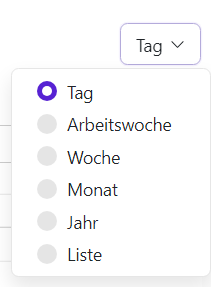
\includegraphics[keepaspectratio]{src/content/docs/user/../../../assets/user/49302f26835d16abbc751105627b819b5d7e3ed0.png}}

}

\caption{Kalender-Ansicht}

\end{figure}%

\section{Eigene, öffentliche und freigegebene
Kalender}\label{eigene-uxf6ffentliche-und-freigegebene-kalender}

In der linken Seitenansicht sehen Sie den Mini-Kalender und in der
Ordneransicht sind Ihre Kalender dargestellt.

\begin{figure}[H]

{\centering \pandocbounded{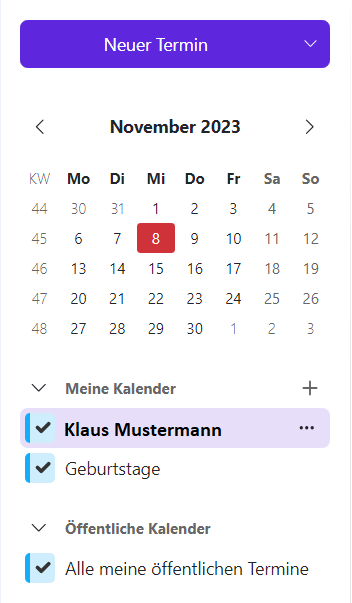
\includegraphics[keepaspectratio]{src/content/docs/user/../../../assets/user/7f2d579c22706f18d47a249aade3520b3fbdafbf.png}}

}

\caption{Kalender-Ordneransicht}

\end{figure}%

\subsection{Mein Kalender}\label{mein-kalender}

Über das Plus (+) neben \textbf{Meine Kalender} können Sie einen neuen
Kalender erstellen, in dem Sie \textbf{Neuen Kalender hinzufügen}
klicken oder für andere Zwecke auf \textbf{Neuen Ressourcenkalender
hinzufügen} und \textbf{Neue Ressourcennkalendergruppe hinzufügen}
klicken.

\begin{figure}[H]

{\centering \pandocbounded{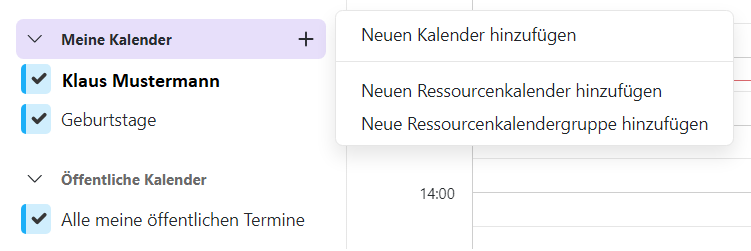
\includegraphics[keepaspectratio]{src/content/docs/user/../../../assets/user/28d50266f65f5cdcb9ede6f73a7699e9ab6b9f44.png}}

}

\caption{Neuer Kalender hinzufügen}

\end{figure}%

\subsection{Öffentliche Kalender}\label{uxf6ffentliche-kalender}

Über \textbf{Öffentliche Kalender} werden alle öffentlichen Termine und
freigegebene Kalender angezeigt.

\section{Die Kalender-Werkzeugleiste}\label{die-kalender-werkzeugleiste}

\subsection{Der Kalender und die
Werkzeugleiste}\label{der-kalender-und-die-werkzeugleiste}

Die Benutzeroberfläche des Kalenders bietet Ihnen die Möglichkeit, einen
Überblick über alle geplanten Termine zu bekommen. Über die
gekennzeichnete Schaltfläche mit den 9 Punkten (\textbf{Alle
Applikationen}) ist es Ihnen möglich, die Programme des Hauptmenüs
auszuwählen, falls Sie zu einer anderen Anwendung wechseln möchten.

\begin{figure}[H]

{\centering \pandocbounded{\includegraphics[keepaspectratio]{src/content/docs/user/../../../assets/user/0e6beaf2b198f9dd0f325bce6361060ba167c795.PNG}}

}

\caption{Alle Applikationen}

\end{figure}%

Die \textbf{Kalender-Werkzeugleiste} enthält folgende Funktionen: -
Neuer Termin: Anlegen eines neuen Termins - Heute: Wechsel auf das
aktuelle Datum in der Kalenderansicht

Ansicht: Wechsel auf Tag, Arbeitswoche, Woche oder Monat Die Funktion
\textbf{Heute} ist jedoch nur verfügbar, wenn Sie als \textbf{Ansicht}
Tag, Arbeitswoche, Woche oder Monat geöffnet haben.

\begin{figure}[H]

{\centering \pandocbounded{\includegraphics[keepaspectratio]{src/content/docs/user/../../../assets/user/f54f6867831d533f667d97e3f3b4aa7c062f77e5.png}}

}

\caption{Kalender-Werkzeugleiste}

\end{figure}%

\section{Termin einstellen}\label{termin-einstellen}

Hier erfahren Sie, wie Sie Ihre Termine erstellen können. Beispielsweise
können Sie Termine mit Videokonferenzen erstellen sowie
Termineinladungen beantworten oder ganze Terminserien einrichten.

So können Sie einen neuen Termin anlegen:

Zuerst öffnen Sie in der Ordneransicht einen Kalender, in dem Sie die
Berechtigung zum Anlegen von Objekten haben. Danach klicken Sie in der
Werkzeugleiste auf \textbf{Einladen}.

\begin{figure}[H]

{\centering \pandocbounded{\includegraphics[keepaspectratio]{src/content/docs/user/../../../assets/user/7d134685fb15ce8a11d32d8799a40491c4988ce3.jpg}}

}

\caption{Neuer Termin}

\end{figure}%

Zuerst müssen Sie einen \textbf{Titel} eingeben.

\begin{figure}[H]

{\centering \pandocbounded{\includegraphics[keepaspectratio]{src/content/docs/user/../../../assets/user/c3c074f213189c8717c5a129058fa94300676395.png}}

}

\caption{Neuen Termin anlegen, Titel festlegen}

\end{figure}%

Um den Beginn und das Ende des Termins festzulegen, müssen Sie unterhalb
von \textbf{Beginnt am} und \textbf{Endet am} folgenden Aktionen
ausführen:

\begin{itemize}
\tightlist
\item
  Klicken Sie auf ein Datum. Geben Sie ein Datum ein oder wählen Sie ein
  Datum aus der Datumsauswahl. Bei ganztägigen Terminen aktivierst du
  \textbf{Ganztägig}
\item
  Klicken Sie auf eine Uhrzeit. Geben Sie die Uhrzeit ein, oder wählen
  Sie eine Uhrzeit aus der Liste
\item
  Wenn gewünscht, können Sie die Zeitzone für die Start- oder Endzeit
  festlegen, indem Sie neben einer Uhrzeit auf die
  Zeitzonen-Schaltfläche klicken. Sie können für die Startzeit und
  Endzeit unterschiedliche Zeitzonen angeben
\end{itemize}

\begin{figure}[H]

{\centering \pandocbounded{\includegraphics[keepaspectratio]{src/content/docs/user/../../../assets/user/0fa0bea2547a7fa7e8d5ab0125760928c5543743.png}}

}

\caption{Termin anlegen, Uhrzeit festlegen}

\end{figure}%

Geben Sie bei Bedarf nun den \textbf{Ort} und eine \textbf{Beschreibung}
ein.

Unter \textbf{Teilnehmer und Ressourcen} haben Sie die Option, weitere
Teilnehmerinnen und Teilnehmer für den Termin einzuladen. Außerdem sehen
Sie unter \textbf{Teilnehmer} , welche Teilnehmerinnen und Teilnehmer
sich bereits in dem Termin befinden. Um weitere Teilnehmerinnen und
Teilnehmer in diesen Termin einzuladen, klicken Sie dafür neben dem Feld
\textbf{Teilnehmer und Ressourcen} auf das Symbol \textbf{Kontakt
auswählen}.

\begin{figure}[H]

{\centering \pandocbounded{\includegraphics[keepaspectratio]{src/content/docs/user/../../../assets/user/32bcf18d4e463be7c7c4477deb841b3770048ce9.jpg}}

}

\caption{Termin Anlegen}

\end{figure}%

Nun öffnet sich ein neues Fenster mit Ihren Kontakten. Möchten Sie
Kontakte hinzufügen, tippen Sie in das Eingabefeld \textbf{Suchen} den
entsprechenden Namen des Kontakts ein und wählen ihn anschließend aus.
Die ausgewählten Kontakte haben nun einen grauen Hintergrund. Klicke auf
\textbf{Wählen} um deine gewünschten Kontakte zu dem Termin
hinzuzufügen. Sie haben außerdem die Möglichkeit Kontakte zu filtern und
in Ihren verschiedenen Adressbüchern nach Kontakten zu suchen. Die
Schaltflächen befinden sich jeweils rechts neben dem Eingabefeld
\textbf{Suchen}.

\begin{figure}[H]

{\centering \pandocbounded{\includegraphics[keepaspectratio]{src/content/docs/user/../../../assets/user/210167904fea7e4d14104273f77f8b0db392a3b1.png}}

}

\caption{Globale Adressliste, Suchen, Filtern, Adressliste}

\end{figure}%

Wenn Sie die Sichtbarkeit Ihres Termins einstellen möchten, können Sie
unter \textbf{Sichtbarkeit} auf den rechten Pfeil in der Schaltfläche
klicken und \textbf{Standard}, \textbf{Privat} oder \textbf{Geheim}
auswählen. Sie können außerdem eine \textbf{Erinnerung} für den Termin
angeben, sodass die entsprechende Teilnehmerin bzw. der entsprechende
Teilnehmer an den Termin erinnert wird. Sie können den gewünschten
Kalender auswählen, in dem der Termin erscheinen soll und sie können die
\textbf{Terminfarbe} auswählen, in der der Termin angezeigt werden soll.
Darüber hinaus haben Sie die Option eine Kategorie Ihres Termins
anzugeben, welche Ihnen erscheint, wenn Sie auf den rechten Pfeil neben
\textbf{Kategorie hinzufügen} klicken. Die Kategorien sind
voreingestellt und es kann \textbf{Predefined}, \textbf{Important},
\textbf{Business}, \textbf{Private} und \textbf{Meeting} ausgewählt
werden. Um dem Termin Anhänge hinzuzufügen, klicken Sie entweder auf
\textbf{Anhänge hinzufügen} oder \textbf{Von Dateien hinzufügen.}

\begin{figure}[H]

{\centering \pandocbounded{\includegraphics[keepaspectratio]{src/content/docs/user/../../../assets/user/e06e3c18927a25b8337c68829d9e054d963b8caa.png}}

}

\caption{Termin anlegen, weitere Funktionen}

\end{figure}%

Haben Sie nun Ihren Termin fertig konfiguriert, müssen Sie ihn noch
speichern. Sie speichern den Termin, indem Sie auf \textbf{Anlegen}
klicken.

\begin{figure}[H]

{\centering \pandocbounded{\includegraphics[keepaspectratio]{src/content/docs/user/../../../assets/user/eec945390db2dadcddff544789b3e1e658e88067.png}}

}

\caption{Termin anlegen}

\end{figure}%

\textbf{Hinweis}: Termine können auch direkt aus dem Kontaktemodul
heraus angelegt werden. Sehen Sie dazu ``Kontakt zu einem Termin
einladen''.

\subsection{Termin mit Videokonferenz}\label{termin-mit-videokonferenz}

Für einen Termin mit mehreren Personen können Sie einen
Videokonferenzraum einrichten. Dabei wird ein Link für den geplanten
Konferenzraum generiert und ein Raum im Modul \textbf{Videokonferenzen}
eingerichtet.

\begin{figure}[H]

{\centering \pandocbounded{\includegraphics[keepaspectratio]{src/content/docs/user/../../../assets/user/a7523b815151e29fb5eac8f69e29d6c9ac9a250b.png}}

}

\caption{Videokonferenz anlegen}

\end{figure}%

\subsection{Serientermin einstellen}\label{serientermin-einstellen}

Möchtest Sie, dass ein Termin regelmäßig in einem bestimmten zeitlichen
Intervall stattfindet, können Sie einen Serientermin einrichten.
Aktivieren Sie dafür \textbf{Wiederholen.} Nun erscheint der aktuelle
Wochentag in violetter Schrift.

Möchten Sie die Wiederholungszeit verändern, klicken Sie auf den
violetten Wochentag

\begin{figure}[H]

{\centering \pandocbounded{\includegraphics[keepaspectratio]{src/content/docs/user/../../../assets/user/f2f3ae67eb45b3886d71114c70e33485f329648d.png}}

}

\caption{Serientermin bearbeiten}

\end{figure}%

Es öffnet sich ein neues Fenster. Hier können nun die terminlichen
Aspekte des Termins bearbeitet werden. Haben Sie Ihre gewünschten
Änderungen vorgenommen, klicken Sie auf \textbf{Anwenden}.

\begin{figure}[H]

{\centering \pandocbounded{\includegraphics[keepaspectratio]{src/content/docs/user/../../../assets/user/752246ddbac3d55756bb09a34dbbd16bf59c6570.png}}

}

\caption{Serientermin bearbeiten}

\end{figure}%

\subsection{Terminsichtbarkeit
einstellen}\label{terminsichtbarkeit-einstellen}

Sie haben die Möglichkeit, Ihren Termin für andere Nutzerinnen und
Nutzer zu verbergen. Wenn Sie möchten, dass andere Nutzerinnen und
Nutzer diesen Termin einsehen können, wählen Sie \textbf{Standard} aus.
Möchten Sie, dass der Termin von anderen Nutzerinnern und Nutzern nicht
eingesehen werden kann, wählen Sie \textbf{Privat} oder \textbf{Geheim}
aus.

\textbf{Privat:} Nutzerinnen und Nutzer, die nicht am Termin teilnehmen,
sehen nur den Zeitpunkt des Termins, nicht den Inhalt.

\textbf{Geheim:} Nutzerinnen und Nutzer, die nicht am Termin teilnehmen,
wird der Termin nicht angezeigt.

Sie können außerdem eine \textbf{Erinnerung} für den Termin angeben,
sodass die entsprechende Teilnehmerin bzw. der entsprechende Teilnehmer
an den Termin erinnert wird. Sie können den gewünschten Kalender
auswählen, in dem der Termin erscheinen soll und Sie können die
\textbf{Terminfarbe} auswählen, in der der Termin angezeigt werden soll.

Darüber hinaus haben Sie die Option eine Kategorie Ihres Termins
anzugeben, welche Ihnen erscheint, wenn Sie auf den rechten Pfeil neben
\textbf{Kategorie hinzufügen} klicken. Die Kategorien sind
voreingestellt und es kann \textbf{Predefined}, \textbf{Important},
\textbf{Business}, \textbf{Private} und \textbf{Meeting} ausgewählt
werden.

Um dem Termin Anhänge hinzuzufügen, klicken Sie entweder auf
\textbf{Anhänge hinzufügen} oder \textbf{Von Dateien hinzufügen.}

\begin{figure}[H]

{\centering \pandocbounded{\includegraphics[keepaspectratio]{src/content/docs/user/../../../assets/user/e06e3c18927a25b8337c68829d9e054d963b8caa.png}}

}

\caption{Sichtbarkeit des Termins}

\end{figure}%

\subsection{Termin planen}\label{termin-planen}

Über \textbf{Planung} können Sie vor Erstellen eines Termins bereits die
Verfügbarkeit der Personen prüfen, die an Ihrem Termin teilnehmen
sollen.

\begin{figure}[H]

{\centering \pandocbounded{\includegraphics[keepaspectratio]{src/content/docs/user/../../../assets/user/0da8c3247f0cbc84961112ab193e4c2921ff7737.png}}

}

\caption{Terminplanung}

\end{figure}%

Über das Feld \textbf{Teilnehmer hinzufügen} können Sie diese auswählen.

\begin{figure}[H]

{\centering \pandocbounded{\includegraphics[keepaspectratio]{src/content/docs/user/../../../assets/user/fe690690bfc960c197a54942fac9f127fd0059e0.png}}

}

\caption{Terminplanung}

\end{figure}%

Haben Sie ein offenes Zeitfenster für alle Beteiligten gefunden, halten
Sie die linke Maustaste gedrückt und ziehen Sie über den gewünschten
Zeitraum im Kalendertag, an dem der Termin stattfinden soll. Klicken Sie
nun auf \textbf{Termin anlegen}. Die von Ihnen zuvor ausgewählte Zeit
wird automatisch in die Felder \textbf{Beginnt am} und \textbf{Endet am}
eingefügt.

\begin{figure}[H]

{\centering \pandocbounded{\includegraphics[keepaspectratio]{src/content/docs/user/../../../assets/user/6597a2a868c1d4a204e99248eeadf8c13e16623b.png}}

}

\caption{Terminplanung}

\end{figure}%

Über \textbf{Optionen} können Sie in diesem Fenster auch Änderungen
vornehmen. So können Sie zum Beispiel über \textbf{Kompakt} die
Darstellung des ausgewählten Kalendertages verkleinern oder über
\textbf{Feinraster anzeigen} den Kalendertag auf viertelstündige Blöcke
aufteilen. Den Datumsbereich können Sie auf Woche oder Monat einstellen.
Sie können ebenfalls bestimmen, ob auch Nichtarbeitszeiten für die
Terminauswahl angezeigt werden sollen oder nicht.

\begin{figure}[H]

{\centering \pandocbounded{\includegraphics[keepaspectratio]{src/content/docs/user/../../../assets/user/cf38b62f477318473e64f15d9757c49b3131d6fd.png}}

}

\caption{Terminplanung Optionen}

\end{figure}%

\subsection{Termineinladung
beantworten}\label{termineinladung-beantworten}

Wurden Sie zu einem Termin eingeladen, erhalten Sie eine oder beide der
folgenden Benachrichtigungen:

\begin{itemize}
\tightlist
\item
  Der Infobereich informiert Sie über diesen Termin
\end{itemize}

Sie erhalten eine E-Mail mit der Termineinladung Termineinladungen
können zugesagt, vorläufig zugesagt oder abgelehnt werden. Dieser
sogenannte Bestätigungsstatus kann auch zu einem späteren Zeitpunkt noch
geändert werden.

\subsubsection{Terminbeantwortung im
Infobereich}\label{terminbeantwortung-im-infobereich}

Wenn Sie die Termineinladung über den Infobereich beantworten möchten,
klicken Sie in der Menüleiste auf das Symbol
\textbf{Benachrichtigungen}. Der Infobereich wird nun angezeigt. Hier
können Sie nun unterhalb der Einladung auf \textbf{Bestätigen,
Vielleicht} oder \textbf{Ablehnen} klicken. Wenn Sie den Termin
bestätigt haben, wird er in Ihrem Kalender eingetragen. Sie können den
Termin auch im Kalender zusagen oder absagen. Klicken Sie dafür im
entsprechenden Tag auf den Termin und beantworten Sie den Termin dort
mit \textbf{Bestätigen}, \textbf{Vielleicht} oder \textbf{Ablehnen}.

\begin{figure}[H]

{\centering \pandocbounded{\includegraphics[keepaspectratio]{src/content/docs/user/../../../assets/user/78cd75b0ad23837318faa679b7ee150ca2893453.png}}

}

\caption{Termineinladung}

\end{figure}%

Wenn Sie auf das Dreipunkte-Menü neben den Antwort-Möglichkeiten
klicken, können Sie eine Bemerkung zum Termin eingeben.

\begin{figure}[H]

{\centering \pandocbounded{\includegraphics[keepaspectratio]{src/content/docs/user/../../../assets/user/cc76ef3e8322e468a48fd82ff94a843724d24027.png}}

}

\caption{Terminbemerkung}

\end{figure}%

\subsubsection{Terminbeantwortung in der
Einladungs-E-Mail}\label{terminbeantwortung-in-der-einladungs-e-mail}

Sie können die Termineinladung auch per E-Mail beantworten. In der App
\textbf{E-Mail} wird die Termineinladung angezeigt. Sie können in der
Detailansicht unterhalb von \textbf{Termindetails anzeigen} einen
Kommentar einfügen. Auch hier haben Sie die Auswahl zwischen
\textbf{Bestätigen, Vielleicht} und \textbf{Ablehnen}. Wie im Abschnitt
„Terminbeantwortung im Infobereich`` beschrieben, wird der Termin in
Ihrem Kalender eingetragen, wenn Sie diesen bestätigen.

\textbf{Hinweis:} In den Kalender-Einstellungen können Sie bestimmen, ob
Einladungs-E-Mails automatisch gelöscht werden sollen, wenn diese von
Ihnen bestätigt oder abgelehnt wurden.

\section{Termin verwalten}\label{termin-verwalten}

Hier erfahren Sie, wie Sie Ihre Termine verwalten. Beispielsweise können
Sie Inhalte von Terminen verändern sowie Termine oder ganze Terminserien
aus dem Kalender löschen.

\subsection{Terminbestätigung
ändern}\label{terminbestuxe4tigung-uxe4ndern}

Sie können Ihre Terminbestätigung auch nachträglich ändern. Dabei gibt
es folgende Optionen:

\begin{itemize}
\tightlist
\item
  Sie können den Termin kommentarlos bestätigen oder ablehnen
\end{itemize}

Sie können den Bestätigungsstatus ändern. Dabei können Sie einen
Kommentar eingeben, den andere Teilnehmerinnen und Teilnehmer des
Termins lesen können.

\textbf{Hinweis:} Je nach Konfiguration Ihrer privaten Kalender können
Sie eine Terminbestätigung nur ändern, wenn Sie selbst teilnehmende
Person des Termins sind.

Sie haben folgende Möglichkeiten, um Ihren Bestätigungsstatus
nachträglich zu ändern:

\begin{itemize}
\tightlist
\item
  Klicken Sie in der Kalenderansicht auf den gewünschten Termin und im
  geöffneten Pop-up auf \textbf{Status ändern}
\end{itemize}

Wählen Sie in der Listenansicht den gewünschten Termin aus und öffnen
ihn mit einem Doppelklick. Klicken Sie anschließend in der
Werkzeugleiste auf \textbf{Status ändern} Handelt es sich um eine
Terminserie, so legen Sie fest, ob die Änderungen nur für einen
einzelnen Termin oder für die gesamte Terminserie gelten sollen. Bei
Bedarf können Sie im Fenster \textbf{Bestätigungsstatus ändern} eine
Anmerkung verfassen. Klicken Sie auf eine der Schaltflächen
\textbf{Ablehnen, Vorläufig} oder \textbf{Akzeptieren}.

\subsection{Terminerinnerung ändern}\label{terminerinnerung-uxe4ndern}

Terminerinnerungen können nachträglich verändert werden, indem Sie eine
Erinnerung anpassen, entfernen oder eine weitere Erinnerung hinzufügen.

\textbf{Hinweis:} Diese Funktion ist nur verfügbar, wenn Sie keine
vollständigen Bearbeitungsrechte für den Termin besitzen. Andernfalls
können Sie die Terminerinnerung ändern, indem Sie das
Terminbearbeitungsfenster verwenden.

Folgende Möglichkeiten haben Sie, um eine Terminerinnerung zu ändern:

\begin{itemize}
\tightlist
\item
  Klicken Sie in der Kalenderansicht auf den gewünschten Termin. Ein
  Pop-up öffnet sich
\end{itemize}

Wählen Sie in der Listenansicht den gewünschten Termin aus. Öffnen Sie
ihn mit einem Doppelklick. Der Termin wird in einem Fenster angezeigt
Klicken Sie nun auf das Symbol \textbf{Weitere Aktionen} und auf
\textbf{Erinnerung ändern}. Das Fenster \textbf{Erinnerungen ändern}
öffnet sich. Wählen Sie eine Erinnerung aus. Dadurch öffnet sich das
Fenster \textbf{Erinnerungen bearbeiten}. Bei Bedarf können Sie jetzt
eine vorhandene Erinnerung bearbeiten, löschen oder eine neue Erinnerung
hinzufügen.

\subsection{Termin als stellvertretende Person anlegen, bearbeiten und
verwalten}\label{termin-als-stellvertretende-person-anlegen-bearbeiten-und-verwalten}

Je nach den Berechtigungen, die Ihnen eine andere nutzende Person
erteilt hat, können Sie in deren Kalender folgende Funktionen ausführen:

\begin{itemize}
\tightlist
\item
  Vorhandene Termine ansehen
\item
  Neue Termine im Namen der nutzenden Person anlegen
\end{itemize}

Vorhandene Termine im Namen der nutzenden Person bearbeiten, verwalten
oder löschen Sie können ebenfalls als stellvertretende Person Termine
anlegen oder bearbeiten. Dafür öffnen Sie in der Ordneransicht unterhalb
von \textbf{Freigegebene Kalender} den Ordner der nutzenden Person, die
Sie zur stellvertretenden Person bestimmt hat. Klicken Sie nun in der
Werkzeugleiste auf \textbf{Neuer Termin}. Sie werden gefragt, ob Sie
diesen Termin als stellvertretende Person im freigegebenen Kalender
einer anderen nutzenden Person anlegen wollen. Klicken Sie auf
\textbf{im Auftrag des Eigentümers}.

Die nutzende Person, für die Sie die Stellvertretung übernehmen, wird
per E-Mail darüber informiert, dass Sie einen Termin angelegt,
bearbeitet oder gelöscht haben. Wie man Termine anlegt, bearbeitet oder
löscht, erfahren Sie im Kapitel \textbf{Termin einstellen}.

\subsection{Organisatorin oder Organisator
ändern}\label{organisatorin-oder-organisator-uxe4ndern}

Wenn Sie die organisierende Person eines (Serien-)Termins sind, der
mindestens 2 weitere Teilnehmende hat, so können Sie die organisierende
Person ändern.

In folgenden Fällen können Sie die organisierende Person nicht ändern:

\begin{itemize}
\tightlist
\item
  Wenn ein Termin externe Teilnehmende hat
\item
  Wenn es sich um einen geänderten Einzeltermin einer Terminserie
  handelt - \textbf{Hinweis:} Diese Funktion ist je nach Konfiguration
  unter Umständen nicht verfügbar.
\end{itemize}

Sie haben folgende Möglichkeiten, die organisierende Person eines
Termins zu ändern:

\begin{itemize}
\tightlist
\item
  Klicken Sie in der Kalenderansicht auf einen Termin. Klicken Sie dann
  im Pop-up auf das Symbol \textbf{Weitere Aktionen}
\end{itemize}

Wählen in der Listenansicht einen oder mehrere Termine aus Klicken Sie
dann in der Werkzeugleiste auf das Symbol \textbf{Weitere Aktionen} und
auf \textbf{Organisator ändern}. Haben Sie eine Terminserie ausgewählt,
müssen Sie festlegen, ob die Änderungen für den einzelnen Termin oder
für die gesamte Terminserie gelten sollen. Im Fenster
\textbf{Organisator ändern} geben Sie nun die E-Mail-Adresse der neuen
Organisatorin oder des neuen Organisators ein.

\subsection{Termin löschen}\label{termin-luxf6schen}

\subsubsection{Termin löschen}\label{termin-luxf6schen-1}

Termine aus Ihren privaten Kalendern können Sie nur löschen, wenn Sie
auch die organisierende Person des Termins sind.

\textbf{Hinweis:} Wenn Sie einen Termin löschen, ist dieser Termin
endgültig gelöscht und kann nicht mehr wiederhergestellt werden.

Sie haben 2 Möglichkeiten, einen Termin zu löschen:

\begin{itemize}
\tightlist
\item
  Klicken Sie in der Kalenderansicht auf den Termin, den Sie löschen
  möchten. Klicken Sie dann im Pop-up auf \textbf{Löschen}
\end{itemize}

Wählen Sie in der Listenansicht einen oder mehrere Termine aus, die Sie
löschen möchten. Klicken Sie dann in der Werkzeugleiste auf
\textbf{Löschen} Bestätigen Sie abschließend, dass Sie den Termin
löschen möchten.

\subsubsection{Serientermine löschen}\label{serientermine-luxf6schen}

Wenn Sie einen Serientermin gewählt haben, werden Sie gefragt, welche
Termine der Terminserie gelöscht werden sollen:

\begin{itemize}
\tightlist
\item
  Wenn Sie den ersten Termin der Terminserie gewählt haben, können Sie
  entweder nur den ersten Termin oder die gesamte Terminserie löschen
\item
  Wenn Sie einen Termin innerhalb der Terminserie gewählt haben, können
  Sie entweder nur den gewählten Termin oder den gewählten Termin und
  alle zukünftigen Termine der Terminserie löschen
\end{itemize}

Wenn Sie den letzten Termin der Terminserie gewählt haben, können Sie
nur den letzten Termin löschen. In diesem Fall werden Sie nicht gefragt,
welche Termine gelöscht werden sollen Wenn Sie gleichzeitig auch die
organisierende Person des Termins sind, können Sie die anderen
Teilnehmerinnen und Teilnehmer über den Grund für die Löschung
informieren, indem Sie eine Nachricht eingeben. Das Eingabefeld wird
angezeigt, wenn folgende Bedingungen erfüllt sind:

\begin{itemize}
\tightlist
\item
  Der Termin hat mindestens 2 Teilnehmende
\end{itemize}

In den Kalender-Einstellungen ist \textbf{Benachrichtigung bei
Terminänderungen} aktiviert. Die Nachricht wird als E-Mail gesendet.

\subsection{Termin in einen anderen Kalender
verschieben}\label{termin-in-einen-anderen-kalender-verschieben}

Sie können Termine in andere Kalender verschieben. Die einzige
Voraussetzung hierfür ist, dass Sie im Zielkalender die Berechtigung zum
Anlegen von Objekten haben.

Sie haben folgende Möglichkeiten, Termine zu verschieben:

\begin{itemize}
\tightlist
\item
  Klicken Sie in der Kalenderansicht auf einen Termin. Klicken Sie dann
  im Pop-up auf das Symbol \textbf{Weitere Aktionen (Drei Punkte)}
\item
  Wählen Sie in der Listenansicht einen oder mehrere Termine aus.
  Klicken Sie dann in der Werkzeugleiste auf das Symbol \textbf{Weitere
  Aktionen (Drei Punkte)}
\end{itemize}

\begin{figure}[H]

{\centering \pandocbounded{\includegraphics[keepaspectratio]{src/content/docs/user/../../../assets/user/60f8f8d972fb0d82d366f4afb1dca2bcb3b54fde.jpg}}

}

\caption{Termin verschieben}

\end{figure}%

Klicken Sie auf \textbf{Verschieben} . Das Fenster \textbf{Verschieben}
öffnet sich. Wählen Sie hier den gewünschten Kalender aus. Bei Bedarf
können Sie auch einen neuen Kalender anlegen, indem Sie auf
\textbf{Ordner anlegen} klicken. Klicken Sie abschließend auf
\textbf{Verschieben}.

\begin{figure}[H]

{\centering \pandocbounded{\includegraphics[keepaspectratio]{src/content/docs/user/../../../assets/user/4e19f51dbcefc4718b2d020e00d2ccdb32f128b2.jpg}}

}

\caption{Termin-verschieben-Zielkalender}

\end{figure}%

\subsection{Termin importieren}\label{termin-importieren}

Wenn eine Datei im iCal-Format vorliegt, können Sie Termine auch
importieren.

Wählen Sie in der Ordneransicht den Kalender aus, in den Sie Termine
importieren möchten. Klicken Sie neben dem Kalender auf das Symbol
\textbf{Aktionen} und auf \textbf{Importieren} . Im Fenster \textbf{Aus
Datei importieren} klicken Sie auf \textbf{Datei hochladen}.

\begin{figure}[H]

{\centering \pandocbounded{\includegraphics[keepaspectratio]{src/content/docs/user/../../../assets/user/aa9809decd7add8f1f6c4ea062a9335abf8a5025.jpg}}

}

\caption{Kalender-importieren-Menue}

\end{figure}%

Wählen Sie nun eine Datei im iCal-Format. Um auch Termine zu
importieren, die die gleiche Identifikationsnummer haben wie bereits
vorhandene Termine, aktivieren Sie vorab \textbf{Vorhandene Termine
ignorieren}. Klicken Sie nun auf \textbf{Importieren}. Die ausgewählten
Termine werden jetzt zu Ihrem Kalender hinzugefügt.

\textbf{Achtung}: Alle Teilnehmerinnen und Teilnehmer der importierten
Termine werden entfernt. Stattdessen werden Sie als teilnehmende Person
hinzugefügt.

\subsection{Termin exportieren}\label{termin-exportieren}

Sie können Termine im Format iCalendar exportieren. Dieses Format können
Sie zum Beispiel verwenden, wenn Sie Termine mit anderen
Kalender-Anwendungen austauschen möchten. Sie können einzelne Termine
oder alle Termine eines Kalenders exportieren.

\subsubsection{Einzeltermin exportieren}\label{einzeltermin-exportieren}

Sie haben folgende Möglichkeiten, einzelne Termine zu exportieren:

\begin{itemize}
\tightlist
\item
  Klicken Sie in der Kalenderansicht auf einen Termin. Klicken dann im
  Pop-up auf das Symbol \textbf{Weitere Aktionen}
\end{itemize}

Wählen Sie in der Listenansicht einen oder mehrere Termine aus. Klicken
Sie dann in der Werkzeugleiste auf das Symbol \textbf{Weitere Aktionen}
Klicken Sie nun auf \textbf{Exportieren}. Es öffnet sich ein Fenster.
Hier wählen Sie die Funktion zum Speichern der Exportdatei.

\subsubsection{Alle Termine exportieren}\label{alle-termine-exportieren}

Wenn Sie alle Termine eines Kalenders exportieren möchten, wählen Sie
zunächst in der Ordneransicht einen persönlichen oder einen öffentlichen
Kalender aus, von dem Sie die Termine exportieren möchten. Klicken Sie
neben dem Ordnernamen auf das Symbol \textbf{Aktionen} und auf
\textbf{Exportieren}. Ein Fenster öffnet sich. Wählen Sie hier die
Funktion zum Speichern der Exportdatei.

\section{Termin drucken}\label{termin-drucken}

Sie können Termine und Kalender ausdrucken. Folgende Möglichkeiten gibt
es: - Sie können ein Kalenderblatt mit Terminen drucken - Sie können die
Daten von Terminen drucken - Sie können eine detaillierte oder kompakte
Liste von Terminen drucken

\subsection{Ein Kalenderblatt drucken}\label{ein-kalenderblatt-drucken}

Um ein Kalenderblatt mit Terminen zu drucken, wählen Sie den gewünschten
Kalender und in der Menüleiste oben rechts die gewünschte
\textbf{Ansicht} (Tag, Arbeitswoche, Woche, Monat, Jahr, Liste) aus.
Öffnen Sie die \textbf{Einstellungen} (Zahnradsymbol) oben rechts neben
Ihrem Profilbild bzw. Namenskürzel. Wählen Sie \textbf{Drucken}. Es wird
eine Druckvorschau angezeigt und Sie können die Druckoptionen des
Druckers anpassen.

\begin{figure}[H]

{\centering \pandocbounded{\includegraphics[keepaspectratio]{src/content/docs/user/../../../assets/user/8f67f756f707878c21d999db984ac5593ea53562.jpg}}

}

\caption{Kalender-Ansichtsauswahl- Arbeitswoche ist ausgewählt}

\end{figure}%%
\begin{figure}[H]

{\centering \pandocbounded{\includegraphics[keepaspectratio]{src/content/docs/user/../../../assets/user/a720f694f06e528c2bbd041e7525bc205a1fef3e.jpg}}

}

\caption{Termin-drucken}

\end{figure}%

\subsection{Daten von Terminen
drucken}\label{daten-von-terminen-drucken}

Um die Daten von Terminen auszudrucken, haben Sie 2 Möglichkeiten:

\begin{itemize}
\tightlist
\item
  Klicken Sie in der Kalenderansicht auf einen Termin. Klicken Sie dann
  im Pop-up auf das Symbol \textbf{Weitere Aktionen} und dann auf
  \textbf{Drucken}
\item
  Wählen Sie in der Listenansicht einen oder mit gedrückter
  \textbf{Strg-Taste} mehrere Termine aus. Klicken Sie dann in der
  Werkzeugleiste auf das Symbol \textbf{Weitere Aktionen} und dann auf
  \textbf{Drucken} . Hier können Sie noch zwischen der kompakten und der
  detaillierten Ansicht zum Drucken wählen
\end{itemize}

\begin{figure}[H]

{\centering \pandocbounded{\includegraphics[keepaspectratio]{src/content/docs/user/../../../assets/user/d75a99e17e8f05d75c0d78b7471e705a41b0438a.jpg}}

}

\caption{Daten-von-Terminen-drucken}

\end{figure}%

\chapter{Projekte}\label{projekte}

Um mit \textbf{Projekte} zu beginnen, gibt es ein paar einfache Schritte
zu befolgen:

\begin{enumerate}
\def\labelenumi{\arabic{enumi}.}
\item
  Neues Projekt erstellen
\item
  Teammitglieder zur Zusammenarbeit einladen
\item
  Arbeitspakete erstellen
\item
  Einrichten eines Projektplans
\end{enumerate}

\section{Self Service}\label{self-service}

\subsection{Meine Seite}\label{meine-seite}

\subsubsection{Überblick}\label{uxfcberblick}

Ihr persönliches Dashboard \textbf{Meine Seite} zeigt Ihnen alle
wichtigen Informationen zu Ihren Projekten an. Sie sehen zum Beispiel
Nachrichten, Ihre Arbeitspakete, gebuchte Zeiten oder einen Kalender.
Selbstverständlich kann Meine Seite nach Ihren Bedürfnissen konfiguriert
werden.

Gehen Sie rechts oben zu Ihrem Profilbild bzw. Namenskürzel und öffnen
Sie das Dropdown-Menü mit einem Klick. Wählen Sie die erste Option
\textbf{Meine Seite} um Ihr Dashboard zu öffnen. In der
Standardeinstellung sehen Sie hier zunächst zwei projektübergreifende
Listen aller \textbf{Arbeitspakete, die Ihnen zugewiesen wurden} und
\textbf{Arbeitspakete, die von Ihnen erstellt wurden}.

\subsubsection{Widgets hinzufügen}\label{widgets-hinzufuxfcgen}

Fügen Sie ein Widget zu \textbf{Meine Seite} hinzu, indem Sie auf das
\textbf{Pluszeichen (+)} oben rechts auf der Seite klicken. Nun werden
auf Ihrer Seite mehrere Pluszeichen sichtbar. Dies sind die Stellen, an
denen Sie neue Widgets hinzufügen können. Entscheiden Sie sich für den
gewünschten Ort und klicken Sie auf das Pluszeichen. Ein neues
Dialogfenster öffnet sich und Sie können aus der Liste der Widgets das
bzw. die gewünschten aussuchen. Durch einen Klick auf den Titel des
Widgets wird dieses direkt eingefügt. Zur Auswahl stehen:

\begin{itemize}
\tightlist
\item
  Arbeitspaket-Tabelle
\item
  Benutzerdefinierter Text
\item
  Dokumente
\item
  Kalender
\item
  Meine gebuchte Zeit
\item
  Mir zugewiesene Arbeitspakete
\item
  Neuigkeiten
\item
  Von mir beobachtete Arbeitspakete
\item
  Von mir erstellte Arbeitspakete
\item
  Von mir verantwortete Arbeitspakete
\end{itemize}

\begin{figure}[H]

{\centering \pandocbounded{\includegraphics[keepaspectratio]{src/content/docs/user/../../../assets/user/38bb61b572cbd51b839f8bb66687a577b378ba33.jpg}}

}

\caption{Widget-hinzufügen}

\end{figure}%

\subsubsection{Position und Größe der Widgets
bearbeiten}\label{position-und-gruxf6uxdfe-der-widgets-bearbeiten}

\textbf{Position}

Ändern Sie die Position eines Widgets auf dem Dashboard mit der Drag \&
Drop-Funktion. Klicken Sie auf die \textbf{Punkte neben dem Titel des
Widgets}. Der Mauszeiger verwandelt sich zu einem Anfasser (Hand).
Ziehen Sie das Widget nun zur gewünschten Stelle.

\textbf{Größe}

Wenn Sie auf die Punkte in der \textbf{unteren rechten Ecke eines
Widgets} klicken, verwandelt sich der Mauszeiger in einen Doppelpfeil.
So können Sie die Größe des Widgets ändern, indem Sie das Widget mit der
Maus entsprechend ziehen.

\subsubsection{Konfigurieren Sie die Ansicht eines Widgets (für
Arbeitspaket-Tabellen)}\label{konfigurieren-sie-die-ansicht-eines-widgets-fuxfcr-arbeitspaket-tabellen}

Optimieren Sie die Ansicht eines Arbeitspakets in den Widgets auf
\textbf{Meine Seite} so, dass nur die von Ihnen benötigten Informationen
angezeigt sind. Klicken Sie in einem Arbeitspaket-Widget auf das
Drei-Punkte-Menü oben rechts und wählen aus dem Dropdown \textbf{Ansicht
konfigurieren}. Im nächsten Fenster wählen Sie die Kriterien für Ihre
Arbeitspakete aus.

\begin{figure}[H]

{\centering \pandocbounded{\includegraphics[keepaspectratio]{src/content/docs/user/../../../assets/user/acf9aef73115a15a20edc65d8ee5741c2d703c71.jpg}}

}

\caption{Ansicht-eines-Widgets-konfigurieren}

\end{figure}%%
\begin{figure}[H]

{\centering \pandocbounded{\includegraphics[keepaspectratio]{src/content/docs/user/../../../assets/user/7d243462e556f88599895d048993d5f42f4eca17.jpg}}

}

\caption{Konfiguration-des-Widgets-für-Arbeitspakete}

\end{figure}%

\subsubsection{Entfernen der Widgets}\label{entfernen-der-widgets}

\textbf{Entfernen} Sie ein Widget von \textbf{Meine Seite}, indem Sie
auf das \textbf{Drei-Punkte-Menü} in der oberen rechten Ecke klicken und
aus dem Dropdown \textbf{Widget entfernen} wählen.

\begin{figure}[H]

{\centering \pandocbounded{\includegraphics[keepaspectratio]{src/content/docs/user/../../../assets/user/247e12e79d865e05bb4cb9d02d0eec9c7582347b.jpg}}

}

\caption{widget-entfernen}

\end{figure}%

\subsubsection{Zeit-Widget}\label{zeit-widget}

Sie können auch ganz bequem Ihre Zeiten auf \textbf{Meine Seite}
eintragen. Fügen Sie dazu das Widget \textbf{Meine gebuchte Zeit} hinzu.
In diesem Widget können Sie direkt neue Zeiteinträge erstellen, indem
Sie auf den Tag klicken, die Zeiten per Drag\&Drop auf ein anderes Datum
ziehen und die Zeiten bearbeiten oder löschen.

\begin{figure}[H]

{\centering \pandocbounded{\includegraphics[keepaspectratio]{src/content/docs/user/../../../assets/user/2cbca8410371a73076c9e51e29037c2bbb820203.jpg}}

}

\caption{Widget-Meine-gebuchte-Zeit}

\end{figure}%

\subsection{Meine Aktivität}\label{meine-aktivituxe4t}

Sie gelangen zu einer Übersicht Ihrer Aktivitäten, indem Sie rechts oben
auf Ihr Profilbild bzw Ihr Namenskürzel navigieren und dort
\textbf{Meine Aktivität} aus dem Dropdown auswählen. Sie sehen nun alle
Ihre aktuellen Aktionen und Projekte, an denen Sie beteiligt sind.

In der Regel sehen Sie zwei Listen:

\begin{itemize}
\tightlist
\item
  \textbf{Projekte} zeigen alle Projekte, in denen Sie Mitglied sind.
\item
  \textbf{Aktivität} zeigt alle Ihre Aktivitäten an, die in Projekte
  aufgezeichnet werden.
\end{itemize}

\textbf{Hinweis:} Bitte beachten Sie, dass nur Aktivitäten von Projekten
angezeigt werden, die das Modul \textbf{Aktivität} aktiviert haben.
Dieses können Sie in den Projektkonfigurationen unter Module vornehmen.

\begin{figure}[H]

{\centering \pandocbounded{\includegraphics[keepaspectratio]{src/content/docs/user/../../../assets/user/a88cf57f2d1bd40dfea48cfe0df48b2db303e931.jpg}}

}

\caption{Aktivität}

\end{figure}%

\subsection{Mein Konto}\label{mein-konto}

Sie finden unter \textbf{Mein Konto} Einstellungen zu Ihrem Account,
indem Sie in der rechten oberen Ecke auf Ihr Profilbild navigieren und
dort Mein Konto aus dem \textbf{Dropdown-Menü} auswählen. Hier sehen Sie
nun folgende Unterpunkte:

\begin{itemize}
\tightlist
\item
  \textbf{Profil}
\item
  \textbf{Einstellungen}
\item
  \textbf{Zwei-Faktor-Authentifizierung}
\item
  \textbf{Zugriffstokens}
\item
  \textbf{Benachrichtigungseinstellungen}
\item
  \textbf{E-Mail-Erinnerungen}
\item
  \textbf{Profilfoto}
\end{itemize}

\subsubsection{Profil}\label{profil}

Sie haben die Möglichkeit Informationen zu Ihrem Profil hinzuzufügen. In
den Zeilen \textbf{Vorname} und \textbf{Nachname} sind diese
vorausgefüllt und können nicht geändert werden. In der Zeile
\textbf{E-Mail} können Sie ihre E-Mail-Adresse einfügen oder ändern.
Außerdem können Sie je nach Bedarf ein Häkchen bei
\textbf{E-Mail-Adresse nicht anzeigen} setzen. Klicken Sie auf
\textbf{Speichern}, um Ihre Profildaten zu speichern.

\begin{figure}[H]

{\centering \pandocbounded{\includegraphics[keepaspectratio]{src/content/docs/user/../../../assets/user/c991bd55d4a9cc36860ca5f19390965a6146275c.png}}

}

\caption{Ansicht Mein Konto}

\end{figure}%

\subsubsection{Einstellungen}\label{einstellungen}

Ändern Sie unter dem Punkt \textbf{Sprache} mittels des Dropdown-Menüs
die Sprache Ihrer Oberfläche. Hier können Sie aus verschiedenen Sprachen
auswählen. Außerdem können Sie Ihre \textbf{Zeitzone} ändern. Es stehen
Ihnen auch hier im Dropdown-Menü verschiedene Zeitzonen zur Verfügung.
Sie können Ihren \textbf{Modus} ändern, indem Sie zwischen \textbf{Hell}
und \textbf{Hell (hoher Kontrast)} entscheiden können. Unter dem Punkt
\textbf{Kommentare anzeigen} können Sie \textbf{Neueste zuerst} oder
\textbf{Älteste zuerst} wählen. Je nach Bedarf können Sie ein Häkchen
bei \textbf{Beim Verlassen einer Arbeitspaket-Seite mit ungespeichertem
Text warnen} und \textbf{Benachrichtigungen erfolgreicher Aktionen
automatisch ausblenden} setzen.

Für die angezeigte Farbe der Aufgaben haben Sie unter \textbf{BACKLOGS}
die Möglichkeit eine Farbe in Form eines Hex-Codes anzugeben und für
Ihre Ansicht können Sie das Häkchen bei \textbf{Zeige Versionen
eingeklappt} aktivieren.

\subsubsection{Zwei-Faktor-Authentifizierung}\label{zwei-faktor-authentifizierung}

Richten Sie für Ihren Account die \textbf{Zwei-Faktor-Authentifizierung}
ein, indem Sie entweder oben rechts auf die Schaltfläche
\textbf{+2FA-Gerät} oder unter dem Punkt \textbf{2FA-Geräte} auf das
\textbf{Plus(+)} klicken. Wenn Sie auf auf eine der beiden Schaltflächen
geklickt haben, befinden Sie sich auf der Seite mit der Überschrift
\textbf{Neues 2FA-Gerät hinzufügen} . Dort können Sie ein neues Gerät
registrieren und sich ein Passwort erstellen, welches von Zeit und Zeit
geändert werden muss. Außerdem können Sie \textbf{2FA Backup-Codes}
erstellen, indem Sie auf \textbf{2FA Backup-Codes generieren} klicken.

\begin{figure}[H]

{\centering \pandocbounded{\includegraphics[keepaspectratio]{src/content/docs/user/../../../assets/user/55a999d2f3eef49dfa6031eb3315f84a93a47661.png}}

}

\caption{Zwei-Faktor-Authentifizierung}

\end{figure}%

\subsubsection{Zugriffstokens}\label{zugriffstokens}

Generieren Sie einen Zugriffstoken, um Drittanbieter-Anwendungen mit
\textbf{Projekte} zu verknüpfen. Um ein neues Token zu erstellen,
klicken Sie auf \textbf{+API-Token}. Sie können außerdem für iCALENDAR,
OAUTH, RSS und den DATEISPEICHER einen Token erstellen. Hierbei wird
jeweils externen Benutzern dieser Anwendungen einen Zugriff auf Ihre
Daten gewährt.

\subsubsection{Sitzungsverwaltung}\label{sitzungsverwaltung}

Sie können eine Liste der Geräte einsehen, mit denen Sie sich mit Ihrem
Konto angemeldet haben. Widerrufen Sie ggfl. Anmeldungen, die nicht von
Ihnen getätigt wurden. Klicken Sie dafür am Zeilenende der jeweiligen
Sitzungen auf das \textbf{Mülltonnen-Symbol}, um diese zu entfernen.

\subsubsection{Benachrichtigungseinstellungen}\label{benachrichtigungseinstellungen}

Nehmen Sie Einstellungen zu Ihren Benachrichtigungen vor. Sie können
jeweils Häkchen aktivieren, um Benachrichtigungen zu Arbeitspaketen und
Projekten zu erhalten, an denen Sie beteiligt oder nicht beteiligt sind.

Außerdem können Sie Benachrichtigungseinstellungen für ein bestimmtes
Projekt hinzufügen, indem Sie auf \textbf{+Einstellung für Projekt
hinzufügen} klicken. Dort können Sie in dem Textfeld \textbf{Bitte
auswählen} den Titel des Projekts eingeben und projektspezifische
Benachrichtigungen vornehmen. Klicken Sie anschließend auf
\textbf{Speichern}, um die Einstellungen beizubehalten.

\begin{figure}[H]

{\centering \pandocbounded{\includegraphics[keepaspectratio]{src/content/docs/user/../../../assets/user/b5578f558a540ffa73513eef7b8956cc76b08913.png}}

}

\caption{Projektspezifische Benachrichtigungseinstellungen}

\end{figure}%

\subsubsection{E-Mail-Erinnerungen}\label{e-mail-erinnerungen}

Unter E-Mail-Erinnerungen können Sie einstellen, ob und welche
Erinnerungs-E-Mails Sie bekommen möchten. Sie können ein Häckchen
setzen, dass Sie eine E-Mail erhalten wollen, wenn Sie jemand erwähnt.
Sie können außerdem entscheiden, wann Sie diese E-Mails erhalten möchten
und wann nicht. Wenn Sie bei \textbf{Tägliche E-Mail-Erinnerungen
aktivieren} den Haken setzen, bekommen Sie täglich
E-Mail-Benachrichtigungen. Geben Sie bitte die gewünschte Zeit für die
E-Mail-Benachrichtigung an.

Sie können auch Tage festlegen, an denen Sie E-Mails bekommen möchten
bzw. keine E-Mails bekommen möchten. Aktivieren Sie dafür die
entsprechenden Wochentage. Wenn Sie tägliche E-Mail-Erinnerungen
vorübergehend pausieren möchten, setzen Sie bitte dort das Häkchen.

Einstellungen für E-Mail-Benachrichtigungen anderer Objekte z.B. wenn
Neuigkeiten, Kommentare, Dokumente, Nachrichten im Forum, Wiki-Seiten
oder Mitgliedschaften hinzugefügt werden, können Sie ebenfalls
vorgenommen werden.

\subsubsection{Profilfoto}\label{profilfoto}

Sie haben unter \textbf{Profilfoto} einen voreingestellten Gravatar. Sie
haben aber die Möglichkeit ihren Gravatar für Ihre E-Mail-Adresse zu
ändern. Klicken Sie dafür auf den folgenden Link:
\href{https://gravatar.com}{gravatar.com}.

Sollten Sie lieber ein selbsterstelltes Profilbild einfügen wollen,
können Sie auf die Schaltfläche \textbf{Datei auswählen} klicken und aus
Ihrem Datenspeicher ein Foto von Ihnen auswählen und dieses hochladen.
Klicken Sie anschließend auf \textbf{Aktualisieren}, um das Foto zu
speichern.

\section{Abmelden}\label{abmelden}

Nachdem Sie sich wie unter \href{erste-schritte}{An- und Abmelden}
beschrieben angemeldet haben, sind die automatisch auch im Modul
\textbf{Projekte} angemeldet. Um sich von diesem Modul abzumelden,
klicken Sie rechts oben auf ihr Profil und wählen Sie die Option
\textbf{Abmelden.}

\begin{figure}[H]

{\centering \pandocbounded{\includegraphics[keepaspectratio]{src/content/docs/user/../../../assets/user/b076c1573f7aa8bf0858539203ae80468f8e9efa.png}}

}

\caption{Abmelden aus dem Modul}

\end{figure}%

\section{Projekte-Modul öffnen}\label{projekte-modul-uxf6ffnen}

Die \textbf{Projektübersicht} öffnen Sie über Ihre persönliche
Startseite. Klicken Sie auf den Module-Button am linken oberen
Bildschirmrand. Der nun offene Reiter zeigt eine Übersicht der
verschiedenen Module. Klicken Sie auf \textbf{Projekte}.

\subsection{Modul-Übersicht}\label{modul-uxfcbersicht}

\begin{figure}[H]

{\centering \pandocbounded{\includegraphics[keepaspectratio]{src/content/docs/user/../../../assets/user/dc81d82a07fe3281ac5d6704ab200f34a5e135c6.PNG}}

}

\caption{Reiter mit Übersicht der Module}

\end{figure}%

\subsection{Projekt-Übersicht}\label{projekt-uxfcbersicht}

\begin{figure}[H]

{\centering \pandocbounded{\includegraphics[keepaspectratio]{src/content/docs/user/../../../assets/user/900d451e2bc8ea788e65ca4a62e7ed7a3a5e6c20.PNG}}

}

\caption{Übersicht der Projekte}

\end{figure}%

\section{Der
Projektmanagement-Lebenszyklus}\label{der-projektmanagement-lebenszyklus}

Das Modul Projekte bietet alle wichtigen Funktionen zur Unterstützung
von Projektteams während des gesamten Projektmanagement-Zyklus.

Das Modul Projekte ermöglicht einen reibungslosen Ablauf der
Projektarbeit und -kommunikation. Von der Idee bis zum Abschluss und der
Dokumentation können Sie alles in Projekte erledigen.

\begin{longtable}[]{@{}
  >{\raggedright\arraybackslash}p{(\linewidth - 2\tabcolsep) * \real{0.1197}}
  >{\raggedright\arraybackslash}p{(\linewidth - 2\tabcolsep) * \real{0.8803}}@{}}
\toprule\noalign{}
\begin{minipage}[b]{\linewidth}\raggedright
Projektphase
\end{minipage} & \begin{minipage}[b]{\linewidth}\raggedright
Dokumentationen für
\end{minipage} \\
\midrule\noalign{}
\endhead
\bottomrule\noalign{}
\endlastfoot
Projektkonzept und -initiierung & Sammeln von Ideen. Festlegung des
Projektumfangs und der zu erbringenden Leistungen. Darunter: Projekt
einrichten, erste Ideen dokumentieren, Projektbeschreibung, Mitglieder
einladen. \\
Projektdefinition und -planung & Erstellen einer Projektübersicht mit
detaillierten Informationen. Anlegen einer Roadmap oder einen
Projektplans \\
Projektstart oder -durchführung & Verwalten Sie alle Projektaktivitäten
wie Aufgaben, Ergebnisse, Risiken, Funktionen, Bugs oder
Änderungswünsche. Verwenden Sie agile Boards mit Ihren Teams,
dokumentieren Sie Meetings oder teilen Sie Neuigkeiten. \\
Projektleistung und -kontrolle & Erstellen und verwalten eines
Projektbudgets. Verfolgung und Bewertung von Zeit und Kosten.
Benutzerdefinierte Berichte für einen genauen, aktuellen Einblick in die
Projektleistung und die zugewiesenen Ressourcen. \\
Projektabschluss & Dokumentieren Sie Projektergebnisse, Gelerntes,
bewährte Praktiken und fassen Sie die wichtigsten Ergebnisse eines
Projekts einfach zusammen. Archivieren Sie Projekte, um später auf
Inhalte und Gelerntes zurückgreifen zu können. \\
\end{longtable}

\subsection{Projektkonzept und
Projektinitiierung}\label{projektkonzept-und-projektinitiierung}

\begin{longtable}[]{@{}
  >{\raggedright\arraybackslash}p{(\linewidth - 2\tabcolsep) * \real{0.2600}}
  >{\raggedright\arraybackslash}p{(\linewidth - 2\tabcolsep) * \real{0.7400}}@{}}
\toprule\noalign{}
\begin{minipage}[b]{\linewidth}\raggedright
Funktionen
\end{minipage} & \begin{minipage}[b]{\linewidth}\raggedright
Dokumentation für
\end{minipage} \\
\midrule\noalign{}
\endhead
\bottomrule\noalign{}
\endlastfoot
Erstellen eines Projekts & Erstellen und Einrichten eines neuen
Projekts \\
Projektstruktur einrichten & Erstellen Sie eine Hierarchie, um Ihre
Arbeit in Projekte zu strukturieren \\
Projekteinstellungen & Erstellen von ersten Ideen, Aufgaben und
Meilensteinen \\
Mitglieder hinzufügen & Teameinladungen verschicken, um gemeinsam an
Projekten zu arbeiten \\
\end{longtable}

\subsubsection{Projekt erstellen}\label{projekt-erstellen}

Sie können ein neues Projekt erstellen, indem Sie auf die violette
Schaltfläche namens \textbf{+Projekt} klicken. Diese befindet sich
direkt auf dem Startbildschirm des Systems im Bereich \textbf{Projekte}.

\begin{figure}[H]

{\centering \pandocbounded{\includegraphics[keepaspectratio]{src/content/docs/user/../../../assets/user/abaf62ae7afdb175bec0ad2e1accb6432a41351b.png}}

}

\caption{Neues Projekt erstellen}

\end{figure}%

Sie können auch ein neues Projekt erstellen, indem Sie auf das violette
\textbf{Pluszeichen (+)} in der oberen Menüleiste klicken.

Ein Menü wird geöffnet. Klicken Sie dann auf \textbf{+Projekt}.

\begin{figure}[H]

{\centering \pandocbounded{\includegraphics[keepaspectratio]{src/content/docs/user/../../../assets/user/62b0064af6f26242e175e333d322575f7665fdac.png}}

}

\caption{Pluszeichen-Menü}

\end{figure}%

Eine neue Seite öffnet sich.

\begin{figure}[H]

{\centering \pandocbounded{\includegraphics[keepaspectratio]{src/content/docs/user/../../../assets/user/7aec3b07f7a7de79d07fc078b0b956fcec38d5cb.png}}

}

\caption{Neues Projekt einstellen}

\end{figure}%

Bei der Erstellung eines neuen Projekts können Sie ein von Grund auf
neues Projekt erstellen oder ein Projekt aus einer \textbf{Vorlage}
erstellen. Im letzteren Fall wählen Sie die Vorlage aus dem
Dropdown-Menü aus.

Geben Sie Ihrem Projekt einen Namen.

Sie können auswählen, ob Ihr Projekt ein \textbf{Unterprojekt} eines
anderen Projekts sein soll. In diesem Fall wählen Sie das Projekt aus
dem Dropdown-Menü aus.

Unter \textbf{Erweiterte Einstellungen} haben Sie die Möglichkeit, Ihrem
Projekt eine Beschreibung hinzuzufügen. Des Weiteren können Sie
bestimmen, ob es öffentlich zugänglich ist und welchen Status es hat,
sowie eine Beschreibung des Status des Projekts eingeben.

\begin{figure}[H]

{\centering \pandocbounded{\includegraphics[keepaspectratio]{src/content/docs/user/../../../assets/user/68dcce2565d8aef6680fe2364c99989868319362.png}}

}

\caption{Erweiterte Einstellungen}

\end{figure}%

Wenn Sie Ihre Projekteinstellungen abgeschlossen haben, klicken Sie auf
die hellviolette Schaltfläche \textbf{Speichern}.

Wenn Sie erfolgreich ein neues Projekt erstellt haben, werden Sie
automatisch zur Projektübersichtsseite weitergeleitet.

\begin{figure}[H]

{\centering \pandocbounded{\includegraphics[keepaspectratio]{src/content/docs/user/../../../assets/user/2cb61a6f7c7e19c0b17093213545d651af1508e3.png}}

}

\caption{Übersichtseite}

\end{figure}%

\textbf{Hinweis}: Wenn Sie ein neues Projekt erstellen, werden Sie
standardmäßig als Projektadministrator festgelegt, unabhängig davon, ob
Sie ein Projekt kopiert, eine Vorlage verwendet oder ein Projekt von
Grund auf neu erstellt haben.

\subsubsection{Einrichten einer
Projektstruktur}\label{einrichten-einer-projektstruktur}

Projekte haben eine klare Struktur, diese umfasst Unterprojekte und
übergeordnete Projekte. Ein Projekt kann zum Beispiel
Organisationseinheiten eines Unternehmens abbilden, um die Vorgänge der
verschiendenen Organisationseinheiten von einander zu trennen. Zum
Beispiel:

\begin{itemize}
\tightlist
\item
  \textbf{Unternehmen (übergeordnetes Projekt)}

  \begin{itemize}
  \tightlist
  \item
    Marketing (Unterprojekt)
  \item
    Vertrieb
  \item
    HR
  \item
    IT
  \item
    \ldots{}
  \end{itemize}
\end{itemize}

Die Projekte können auch für Teams verwendet werden, die an einem
gemeinsamen Thema arbeiten. Zum Beispiel:

\begin{itemize}
\tightlist
\item
  \textbf{Einführung eines neuen Produkts}

  \begin{itemize}
  \tightlist
  \item
    Design
  \item
    Entwicklung
  \item
    \ldots{}
  \end{itemize}
\end{itemize}

Ein Projekt kann sich auch auf einzelne Produkte oder Kunden beziehen.
Zum Beispiel:

\begin{itemize}
\tightlist
\item
  \textbf{Produkt A}

  \begin{itemize}
  \tightlist
  \item
    Kunde A
  \item
    Kunde B
  \item
    Kunde C
  \end{itemize}
\end{itemize}

Projekte werden in diesem Modul verwendet, um die relevanten Module und
Plugins zu strukturieren. Der Screenshot unten zeigt ein
Entwicklungsprojekt.

\begin{figure}[H]

{\centering \pandocbounded{\includegraphics[keepaspectratio]{src/content/docs/user/../../../assets/user/d9dc09a87e808229025cfc66ffdb8137e015023c.png}}

}

\caption{Projektstruktur}

\end{figure}%

\textbf{Hinweis}: Sie müssen Mitglied eines Projekts sein, um das
Projekt zu sehen und in einem Projekt arbeiten zu können.

\subsubsection{Projekt-Einstellungen}\label{projekt-einstellungen}

In den erweiterten Einstellungen der Projektkonfiguration haben Sie die
Möglichkeit, zusätzliche Konfigurationsoptionen festzulegen. Um zur
Projektkonfiguration zu gelangen, gehen Sie wie folgt vor: Wählen Sie
zunächst das gewünschte Projekt aus, klicken Sie dann auf
\textbf{Projektkonfiguration} und anschließend auf
\textbf{Informationen}.

Dort können Sie festlegen, ob dieses Projekt als übergeordnetes Projekt
betrachtet werden soll, indem Sie die Option \textbf{Unterprojekt von}
aktivieren. Auf diese Weise können Sie die Struktur Ihrer
Projekthierarchie nach Ihren Wünschen anpassen.

Es ist wichtig, eine ausführliche Beschreibung für Ihr Projekt
bereitzustellen, und Sie können auch die Standard-Projektkennung
einsehen, die in der URL angezeigt wird.

Bitte beachten Sie, dass das Ändern der Projektkennung eines bereits
bearbeiteten Projekts erhebliche Auswirkungen auf die Zusammenarbeit
haben kann und daher nicht empfohlen wird. Zum Beispiel kann es dazu
führen, dass Repositories nicht ordnungsgemäß geladen werden und Deep
Links nicht mehr funktionieren, da sich die Projekt-URL ändert, wenn die
Projektkennung geändert wird.

Falls gewünscht, können Sie Ihr Projekt auch auf \textbf{öffentlich}
setzen, was bedeutet, dass darauf ohne Anmeldung bei Projekten
zugegriffen werden kann. Vergessen Sie nicht, Ihre Änderungen durch
Klicken auf den violetten \textbf{Speichern} Button zu sichern. Sie
können auch die Autovervollständigung verwenden, um die Projektattribute
schnell und einfach auszufüllen.

\begin{figure}[H]

{\centering \pandocbounded{\includegraphics[keepaspectratio]{src/content/docs/user/../../../assets/user/477a893949c1d55dd3a8c15f9562dbdd77ccf2ec.jpg}}

}

\caption{Neues Projekt erstellen}

\end{figure}%

\paragraph{Projekthierarchie ändern}\label{projekthierarchie-uxe4ndern}

Um die Hierarchie des Projekts zu ändern, navigieren Sie zu den
\textbf{Projektkonfiguration}, genauer gesagt zu \textbf{Informationen},
und passen Sie die Angaben im \textbf{Unterprojekt von} Feld an.

Anschließend betätigen Sie den violetten \textbf{Speichern} Button, um
Ihre Anpassungen zu sichern.

\begin{figure}[H]

{\centering \pandocbounded{\includegraphics[keepaspectratio]{src/content/docs/user/../../../assets/user/a21a8549bc31322e2d5a6d7dc3a6283a8f780677.jpg}}

}

\caption{Unterprojekt von}

\end{figure}%

\paragraph{Ein Projekt auf öffentlich
setzen}\label{ein-projekt-auf-uxf6ffentlich-setzen}

Möchten Sie Ihr Projekt öffentlich zugänglich machen, markieren Sie
einfach das Kontrollkästchen neben \textbf{Öffentlich} in den
\textbf{Projektkonfiguration} unter Informationen.

Die Einstellung \textbf{Öffentlich} ermöglicht allen Benutzern innerhalb
Ihrer Projekte-Instanz den Zugriff auf das Projekt.

(Wenn Ihre Instanz \textbf{ohne Authentifizierung zugänglich} ist, wird
durch diese Option das Projekt auch für die breite Öffentlichkeit
sichtbar, unabhängig von registrierten Benutzerinnen und Benutzern.)

\paragraph{Projekt kopieren}\label{projekt-kopieren}

Um ein bereits existierendes Projekt zu duplizieren, navigieren Sie zu
den \textbf{Projektkonfiguration} und klicken Sie oben rechts in den
\textbf{Projektkonfiguration} auf die Option \textbf{Kopieren}.

\begin{figure}[H]

{\centering \pandocbounded{\includegraphics[keepaspectratio]{src/content/docs/user/../../../assets/user/8d7d22931fdef58d65e77814945a9ec7a3561610.jpg}}

}

\caption{Kopieren}

\end{figure}%

Benennen Sie das neue Projekt, bestimmen Sie, welche Module und
Konfigurationseinstellungen Sie duplizieren möchten, und entscheiden
Sie, ob Sie die Projektmitglieder per E-Mail über den Kopiervorgang
informieren möchten oder nicht. Zudem haben Sie die Möglichkeit,
vorhandene Boards (außer dem Subprojekt-Board) sowie die
\textbf{Projektübersicht} in Ihr neues Projekt zu übernehmen.

\begin{figure}[H]

{\centering \pandocbounded{\includegraphics[keepaspectratio]{src/content/docs/user/../../../assets/user/153bd21eab2d0600e1a07812e06d481708722292.jpg}}

}

\caption{Kopieren}

\end{figure}%

\textbf{Hinweis}: dass \textbf{Budgets} nicht kopiert werden können.
Daher sollten Sie diese zuvor aus der Arbeitspaket-Tabelle entfernen.
Alternativ können Sie die Budgets auch im Budget-Modul löschen, was
gleichzeitig deren Entfernung aus den Arbeitspaketen bewirkt.

Für weitere Anpassungen stehen Ihnen die \textbf{erweiterten
Einstellungen} zur Verfügung. Hier haben Sie die Möglichkeit,
verschiedene Aspekte festzulegen, darunter die URL (Kennung) des
Projekts, seine Sichtbarkeit und seinen Status. Zusätzlich können Sie
Werte für benutzerdefinierte Felder definieren (im Screenshot nicht
dargestellt).

\begin{figure}[H]

{\centering \pandocbounded{\includegraphics[keepaspectratio]{src/content/docs/user/../../../assets/user/aabce3ee6a118e2e36c0dce296afb5844f6edac5.png}}

}

\caption{Projekt Kopieren}

\end{figure}%

\paragraph{Projekt archivieren}\label{projekt-archivieren}

Wenn Sie ein Projekt archivieren möchten, begeben Sie sich zu den
\textbf{Projektkonfiguration} und betätigen Sie \textbf{Archivieren}.

\textbf{Hinweis:} Diese Option steht immer für Mitglieder der Instanz-
und Projektadministration zur Verfügung. Unter Umständen kann sie auch
für bestimmte Rollen aktiviert werden, indem die Berechtigung zur
Projektarchivierung über die \textbf{Einstellungen für Rollen und
Berechtigungen} in den Administrations-Einstellungen aktiviert wird.

\begin{figure}[H]

{\centering \pandocbounded{\includegraphics[keepaspectratio]{src/content/docs/user/../../../assets/user/05b5b570563f661ce307cb8b32a4090c42d874e0.jpg}}

}

\caption{Archivieren}

\end{figure}%

Nachdem dies getan ist, wird das Projekt nicht mehr in der Liste der
auswählbaren Projekte angezeigt. Es bleibt jedoch weiterhin im
\textbf{Alle Projekte anzeigen} Dashboard verfügbar, sofern Sie den
\textbf{Aktiv} Filter auf \textbf{aus} setzen, indem Sie den
Schieberegler nach links verschieben. Hier haben Sie die Möglichkeit,
die Archivierung rückgängig zu machen, indem Sie auf die drei Punkte am
rechten Ende einer Zeile klicken und \textbf{Entarchivieren} auswählen.

\begin{figure}[H]

{\centering \pandocbounded{\includegraphics[keepaspectratio]{src/content/docs/user/../../../assets/user/187282835f50c13a017dbdaa5b09d22bd67beff9.jpg}}

}

\caption{Aktiv}

\end{figure}%

\paragraph{Ein Projekt löschen}\label{ein-projekt-luxf6schen}

Falls Sie ein Projekt löschen möchten, begeben Sie sich bitte zur
\textbf{Projektkonfiguration} und betätigen Sie \textbf{Löschen}. Dies
befindet sich oben rechts auf der Seite.

\begin{figure}[H]

{\centering \pandocbounded{\includegraphics[keepaspectratio]{src/content/docs/user/../../../assets/user/54d901a522c0133af391cb3e1b1df8a4638ebd14.jpg}}

}

\caption{Löschen}

\end{figure}%

Es besteht auch die Möglichkeit, ein Projekt über die Projektübersicht
zu entfernen.

\textbf{Hinweis}: Das Löschen von Projekten ist ausschließlich
Systemadministratoren vorbehalten.

\subsubsection{Mitglieder hinzufügen}\label{mitglieder-hinzufuxfcgen}

Zur Ansicht und Bearbeitung eines Projekts müssen Sie Mitglied eines
Projekts sein. Aus diesem Grund ist das Hinzufügen von Teammitgliedern
zu einem Projekt erforderlich. Ein \textbf{Mitglied} wird als
Projektmitglied innerhalb eines Projekts definiert. Projektmitglieder
können im Modul \textbf{Mitglieder} des Projektmenüs hinzugefügt werden.

\textbf{Hinweis}: Sind Sie kein Projektmitglied, erscheint das Projekt
nicht in der Projektauswahl oder in der Projektliste.

\paragraph{Mitglieder ansehen}\label{mitglieder-ansehen}

Wählen Sie im Projektmenü das Modul \textbf{Mitglieder}, um eine Liste
aller \textbf{Projektmitglieder} und ihrer \textbf{Rollen} im Projekt
anzuzeigen.

Einen Überblick über die aktuellen Mitglieder dieses Projekts finden Sie
in der Mitgliederliste oder im Mitglieder-Widget auf der
Übersichtsseite.

\begin{figure}[H]

{\centering \pandocbounded{\includegraphics[keepaspectratio]{src/content/docs/user/../../../assets/user/3d8b3db96e861b4b2c0d2624d488c89b91de2bcf.png}}

}

\caption{Übersichtseite eines Projektes}

\end{figure}%

\paragraph{Bestehende Konten
hinzufügen}\label{bestehende-konten-hinzufuxfcgen}

Wählen Sie zuerst das Projekt aus, zu dem Sie Mitglieder hinzufügen
möchten, um bestehende Konten oder Gruppen zu einem Projekt
hinzuzufügen. Dies können Sie tun, indem Sie das Modul
\textbf{Mitglieder} auf der linken Seite des Projektmenüs auswählen.
Eine andere Möglichkeit ist, auf \textbf{+Mitglied} im Mitglieder-Widget
auf der Projektübersichtsseite zu klicken.

\begin{figure}[H]

{\centering \pandocbounded{\includegraphics[keepaspectratio]{src/content/docs/user/../../../assets/user/eb30f555bb2d0c611a346993b8f61bb714724fdd.png}}

}

\caption{Mitglieder hinzufügen}

\end{figure}%

Klicken Sie auf die violette Schaltfläche \textbf{+Mitglied} oben
rechts. Tippen Sie den Namen der Person oder der Gruppe ein, die Sie zum
Projekt hinzufügen möchten. Es können mehrere Mitglieder gleichzeitig
ausgewählt und hinzugefügt werden. Den neuen Mitgliedern eine Rolle
zuweisen (\textbf{Mitglied}, \textbf{Leser} oder \textbf{Projekt-Admin})
und auf die hellviolette Schaltfläche \textbf{Hinzufügen} klicken.

\textbf{Hinweis}: Klicken Sie auf den Namen des neuen Mitglieds oder
drücken Sie die Eingabetaste, bevor Sie auf die Schaltfläche
\textbf{Hinzufügen} klicken.

\paragraph{Neue Mitglieder einladen}\label{neue-mitglieder-einladen}

Sie können auch Mitglieder zu einem Projekt einladen, die noch kein
Konto haben. Dafür gibt es drei Möglichkeiten:

\begin{itemize}
\tightlist
\item
  Über das Mitgliedermodul einladen
\item
  Aus der Kopfleiste einladen
\item
  Mitglieder aus einem Arbeitspaket einladen
\end{itemize}

\subparagraph{Einladung von Personen im
Mitglieder-Modul}\label{einladung-von-personen-im-mitglieder-modul}

Folgen Sie den Schritten wie im \textbf{Bereich Bestehenden Konten
hinzufügen} (s. o.). Anstatt eines beliebigen Namens geben Sie die
E-Mail-Adresse des neuen Mitglieds ein. Findet Projekte kein bestehendes
Konto, wird automatisch die Information \textbf{Einladung an\ldots{}
senden} gesetzt. Drücken Sie die \textbf{Eingabetaste} oder wählen Sie
den Text \textbf{Einladung an\ldots{} senden}. Weisen Sie dem neuen
Mitglied eine Rolle zu und klicken Sie auf die violette Schaltfläche
\textbf{Hinzufügen}.

Der Benutzer wird per E-Mail eine Einladung mit einem \textbf{Link}
erhalten, um einen Account für Projekte zu erstellen.

\begin{figure}[H]

{\centering \pandocbounded{\includegraphics[keepaspectratio]{src/content/docs/user/../../../assets/user/6f6531b943094f5aeb1778d88eba775678379f4d.png}}

}

\caption{Neue Mitglieder einladen}

\end{figure}%

\subparagraph{Einladung von Personen aus der
Kopfleiste}\label{einladung-von-personen-aus-der-kopfleiste}

In der immer vorhandenen Kopfzeile finden Sie eine violettes
Plus-Symbol. Diese Schaltfläche ermöglicht es Ihnen, Projekte und
Arbeitspakete zu erstellen sowie Benutzer einzuladen, wo auch immer Sie
sich in der Anwendung befinden.

\begin{figure}[H]

{\centering \pandocbounded{\includegraphics[keepaspectratio]{src/content/docs/user/../../../assets/user/d8b82f1aeeea9b820297146c7c762846b8702e87.png}}

}

\caption{Mitglieder einladen durch Kopfleiste}

\end{figure}%

Sobald Sie auf \textbf{Nutzer einladen} geklickt haben, erscheint ein
Pop-up-Fenster, in dem Sie einstellen können, zu welchem Projekt Sie die
neuen Mitglieder hinzufügen und welche Rollen sie erhalten. Klicken Sie
auf \textbf{Weiter}, wenn Sie alle Daten eingegeben haben. Bevor die
Einladung versendet wird, sehen Sie die Angaben zur Kontrolle. Wenn
alles in Ordnung ist, klicken Sie auf \textbf{Einladung senden}. Eine
Bestätigung wird angezeigt. Klicken Sie auf \textbf{Fortfahren}. Sie
werden sofort zur Mitgliederliste weitergeleitet.

\textbf{Achtung}: Wenn Sie das Popup-Fenster im letzten Schritt
schließen, werden die Daten \textbf{nicht} gespeichert und die Einladung
wird \textbf{nicht} versendet.

\begin{figure}[H]

{\centering \pandocbounded{\includegraphics[keepaspectratio]{src/content/docs/user/../../../assets/user/3483bf8d79ba5a30532239a0e2d4a290af8e9c7e.png}}

}

\caption{Pop-Up Fenster}

\end{figure}%%
\begin{figure}[H]

{\centering \pandocbounded{\includegraphics[keepaspectratio]{src/content/docs/user/../../../assets/user/f0bd79abdc5fcd09d951ad90f83016c1b77d9b3f.png}}

}

\caption{Nutzer einladen}

\end{figure}%%
\begin{figure}[H]

{\centering \pandocbounded{\includegraphics[keepaspectratio]{src/content/docs/user/../../../assets/user/6466bcda4b71d7e72125bc00405f68e60bbfedf6.png}}

}

\caption{Einladung senden}

\end{figure}%%
\begin{figure}[H]

{\centering \pandocbounded{\includegraphics[keepaspectratio]{src/content/docs/user/../../../assets/user/c6a481987cbecb16cb069055e74fb08d90566706.png}}

}

\caption{Bestätigung zur Einladung}

\end{figure}%

\subparagraph{Mitglieder aus einem Arbeitspaket
einladen}\label{mitglieder-aus-einem-arbeitspaket-einladen}

Sie können Mitglieder einladen, indem Sie in der Arbeitspaket-Tabelle
arbeiten. Durch Klicken auf die Spalte \textbf{Zugewiesen an} öffnet
sich ein Dropdown-Menü mit der Option \textbf{Einladen}. Damit können
Sie wie im Abschnitt \hyperref[c5415]{Einladung von Personen aus der
Kopfleiste} (s. o.) vorgehen und z. B. eine Person einladen, die noch
keinen Zugang zu Projekte hat. Das Gleiche gilt für die Buchhaltung oder
benutzerdefinierte Felder für Ihr Projekt.

Sie können jetzt mit Ihrem Team in Projekte zusammenarbeiten. Neu
eingeladene Personen werden mit einem Briefsymbol neben ihrem Namen
angezeigt.

\textbf{Achtung}: Das Entfernen eines Mitglieds, das die Einladung noch
nicht angenommen hat, aus einem Projekt führt zur Löschung des Kontos,
die nicht rückgängig gemacht werden kann.

\begin{figure}[H]

{\centering \pandocbounded{\includegraphics[keepaspectratio]{src/content/docs/user/../../../assets/user/8c15eef1e184cd7454f521bbd26f4d4c34c4aa82.png}}

}

\caption{Einladen aus Arbeitspaket}

\end{figure}%

\paragraph{Verhalten von Gruppen als
Projektmitglieder}\label{verhalten-von-gruppen-als-projektmitglieder}

Gruppen haben die folgenden Auswirkungen auf eine Projektmitgliederliste
und verhalten sich etwas anders als einzelne Konten:

\begin{itemize}
\tightlist
\item
  Der Gruppenname wird in der Projektmitgliederliste in einer eigenen
  Zeile angezeigt
\item
  Die Gruppenmitglieder können nicht einzeln aus der Mitgliederliste
  entfernt werden (kein Löschsymbol)
\item
  Das Hinzufügen einer Gruppe, deren Mitglieder sich bereits in einer
  Projektmitgliedsliste befinden, fügt die Rolle der Gruppe zu deren
  Projektrollen hinzu
\item
  Ein Projektmitglied, das Mitglied einer Gruppe ist, kann einzeln
  weitere Rollen erhalten
\item
  Die Gruppenrolle kann für einzelne Gruppenmitglieder nicht geändert
  werden
\end{itemize}

\subsection{Projektdefinition und
-planung}\label{projektdefinition-und--planung}

Erstellen Sie eine Projektübersicht mit detaillierteren Informationen,
richten Sie Ihren Projektplan ein, strukturieren Sie Ihre Arbeit,
erstellen Sie eine Roadmap.

\subsubsection{Übersicht der globalen
Projekte}\label{uxfcbersicht-der-globalen-projekte}

\paragraph{Übersicht der Projekte}\label{uxfcbersicht-der-projekte}

Ihre Arbeit in dem Modul \textbf{Projekte} kann in mehreren Projekten
organisiert werden, jedes mit einer bestimmten Anzahl von Mitgliedern
und deren jeweiligen Rollen in diesem Projekt. Jedes Projekt wiederum
kann individuell konfiguriert werden. In Bezug auf die aktivierten
Funktionen werden Projekte auch als Module bezeichnet. Diese
Unterscheidung zwischen den Projekten bietet Ihnen viel Flexibilität bei
der Einrichtung Ihrer Arbeit und der Kontrolle darüber, was die
Benutzerinnen und Benutzer in jedem einzelnen Projekt sehen und/oder
bearbeiten dürfen.

Um mehr über die Erstellung und Verwaltung von Projekten zu erfahren,
besuchen Sie bitte unseren separaten Abschnitt \textbf{Projekte
verwalten}.

\subsubsection{Strukturierung der
Arbeit}\label{strukturierung-der-arbeit}

Auf dieser Seite erhalten Sie eine Einführung in die
\textbf{Arbeitspakete}. Im Folgenden wird erklärt, was ein
\textbf{Arbeitspaket} ist und wie Sie \textbf{Arbeitspakete} erstellen
und bearbeiten können.

\textbf{Was ist ein Arbeitspaket?}

Ein Arbeitspaket in Projekte kann im Grunde alles sein, was Sie in Ihren
Projekten benötigen, um den Überblick zu behalten. Es kann z. B. eine
Aufgabe, ein Meilenstein oder eine Projektphase sein. Diese
verschiedenen \textbf{Arten von Arbeitspaketen} werden
\textbf{Arbeitspaket-Typen} genannt.

\textbf{Erstellen eines Arbeitspakets}

Klicken Sie innerhalb des Moduls Arbeitspakete auf die \textbf{violette
Schaltfläche + Erstellen} , um ein neues Arbeitspaket zu erstellen.
Wählen Sie im Dropdown-Menü aus, welche Art von Arbeitspaket Sie
erstellen möchten; z. B. eine Aufgabe oder einen Meilenstein. Um ein
neues Arbeitspaket zu erstellen, können Sie auch den \textbf{violett
gedruckten Schriftzug + Neues Arbeitspaket erstellen} wählen.

\begin{figure}[H]

{\centering \pandocbounded{\includegraphics[keepaspectratio]{src/content/docs/user/../../../assets/user/4a32f01877429a2af970ba4fa7959ef425f29681.PNG}}

}

\caption{Übersicht Arbeitspakete}

\end{figure}%

Es öffnet sich eine geteilte Bildschirmansicht mit dem Formular für
\textbf{neue Arbeitspakete} auf der rechten Seite und der Tabelle mit
den bereits vorhandenen Arbeitspaketen auf der linken Seite.

In das leere Formular auf der rechten Seite können Sie alle relevanten
Informationen für dieses Arbeitspaket eingeben, z. B. den Betreff und
eine Beschreibung, ein Fälligkeitsdatum oder ein beliebiges anderes
Feld. Die Felder, die Sie ausfüllen können, werden Arbeitspaketattribute
genannt. Außerdem können Sie Anhänge mit Kopieren und Einfügen oder mit
Drag \& Drop hinzufügen.

Klicken Sie auf die violette Schaltfläche \textbf{Speichern}, um das
Arbeitspaket zu erstellen.

\begin{figure}[H]

{\centering \pandocbounded{\includegraphics[keepaspectratio]{src/content/docs/user/../../../assets/user/f67d02fb707ea1906caa26fb5fd552bb38446e9b.PNG}}

}

\caption{Formular Neue Aufgabe}

\end{figure}%

Das Arbeitspaket öffnet sich anschließend in der Tabellenansicht:

\begin{figure}[H]

{\centering \pandocbounded{\includegraphics[keepaspectratio]{src/content/docs/user/../../../assets/user/671fa2fc5fa32418c33b7bda958474bacb35014d.png}}

}

\caption{Tabellenübersicht Arbeitspakete}

\end{figure}%

Eine weitere Möglichkeit, ein Arbeitspaket zu erstellen, ist die
Erstellung über das \textbf{Headermenü}. Die aktivierten
\textbf{Arbeitspakettypen} werden angezeigt, und Sie können den
entsprechenden Arbeitspakettyp für die Erstellung auswählen.

\begin{figure}[H]

{\centering \pandocbounded{\includegraphics[keepaspectratio]{src/content/docs/user/../../../assets/user/2d63365db6cdfdf8fce213a53f9e6529414cbc9a.PNG}}

}

\caption{Arbeitspaket via Headermenü erstellen}

\end{figure}%

Sobald Sie auf den Typ des Arbeitspakets klicken, den Sie erstellen
möchten, öffnet sich die Detailansicht des Arbeitspakets. Wählen Sie das
Projekt aus, für das Sie das Arbeitspaket erstellen möchten.

\begin{figure}[H]

{\centering \pandocbounded{\includegraphics[keepaspectratio]{src/content/docs/user/../../../assets/user/dacb71cf85c425316e3faac808079d21b07dd52d.PNG}}

}

\caption{Arbeitspaket Detailansicht}

\end{figure}%

Dann folgen Sie den gleichen Schritten wie oben, um die Attribute Ihres
Arbeitspakets auszufüllen und es zu speichern.

\paragraph{Arbeitspakete öffnen und
bearbeiten}\label{arbeitspakete-uxf6ffnen-und-bearbeiten}

Um ein vorhandenes Arbeitspaket aus der Tabelle zu öffnen und zu
bearbeiten, wählen Sie das Arbeitspaket in der Tabelle aus und klicken
Sie auf das Symbol \textbf{Detailansicht öffnen}, um die geteilte
Bildschirmansicht zu öffnen. Sie können auch auf den Info-Button im
oberen Bereich der Tabellenansicht klicken. Ebenso ist es möglich die
Detailansicht per Doppelklick auf das Arbeitspaket zu öffnen.

\begin{figure}[H]

{\centering \pandocbounded{\includegraphics[keepaspectratio]{src/content/docs/user/../../../assets/user/671fa2fc5fa32418c33b7bda958474bacb35014d.png}}

}

\caption{Arbeitspakete Tabelle}

\end{figure}%

Wenn Sie in die Liste auf der linken Seite auf ein Arbeitspaket klicken,
sehen Sie die entsprechenden Details auf der rechten Seite des geteilten
Bildschirms.

Hier kann in ein beliebiges Feld geklickt werden, um Änderungen
vorzunehmen. Sie können z. B. den Text der Beschreibung anpassen.

Anschließend klicken Sie auf den Haken unter dem Feld, um die Änderungen
zu speichern.

\begin{figure}[H]

{\centering \pandocbounded{\includegraphics[keepaspectratio]{src/content/docs/user/../../../assets/user/9d252a2995bf66726162d7f6d23dd61cdaaaa541.png}}

}

\caption{Detailansicht einer Aufgabe}

\end{figure}%

Um den \textbf{Status} zu ändern, klicken Sie in der Detailansicht auf
den aktuellen Status und wählen Sie den neuen Status des Arbeitspakets
im Dropdown-Menü aus.

\paragraph{Aktivität in
Arbeitspaketen}\label{aktivituxe4t-in-arbeitspaketen}

Um über alle Änderungen eines Arbeitspakets auf dem Laufenden zu bleiben
öffnen Sie den \textbf{Aktivitäten-Tab} oben in der Detaillansicht.

Dort können Sie alle Änderungen ansehen, die an dem Paket vorgenommen
wurden. Sie können am Ende der \textbf{Aktivitätenliste} kommentieren
und andere Kolleginnen und Kollegen per ``@'' markieren.

\begin{figure}[H]

{\centering \pandocbounded{\includegraphics[keepaspectratio]{src/content/docs/user/../../../assets/user/21023d4a4264193eea4bba60d634e044fd4bfdf2.png}}

}

\caption{Kommentare in der Aktivitätenübersicht}

\end{figure}%

Andere Kolleginnen und Kollegen können per ``@'' vor dem Nutzernamen
markiert werden, um Sie über Änderungen zu informieren. Die getaggten
Personen erhalten die Meldung im Projekte-Modul.

\subsubsection{Roadmap-Planung - Einführung in
Gantt-Diagramme}\label{roadmap-planung---einfuxfchrung-in-gantt-diagramme}

Hier erhalten Sie erste Einblicke in \textbf{Gantt-Diagramme}. Sie
erfahren wie es Ihnen möglich ist, über \textbf{Gantt-Diagramme} einen
Projektplan zu ertellen und zu organisieren.

\textbf{Gantt-Diagramme} sind im Modul Projekte als eine Art
Balkendiagramm definiert, das alle Aufgaben eines Projekts darstellt.
Die Aufgaben werden vertikal aufgelistet, die horizontale Achse befasst
sich mit der Zeitangabe. Die Länge der Balken ist an die Dauer der
jeweiligen Aufgabe angepasst.

\paragraph{Was ist ein
Gantt-Diagramm?}\label{was-ist-ein-gantt-diagramm}

Mittels \textbf{Gantt-Diagrammen} können Sie einen Projektplan
erstellen, diesen verwalten und die Informationen mit Ihrem Team teilen.
Sie können die für die Umsetzung des Projekts notwendige
Arbeitspaketplanung und die erforderlichen Schritte zur Fertigstellung
Ihres Projekts visualisieren. Nehmen Sie die Rolle der Projektleitung
ein, werden Sie über Verzögerungen informiert und können Maßnahmen
einleiten.

Das dynamsiche \textbf{Gantt-Diagramm} zeigt die Phasen, Aufgaben und
Meilensteine Ihres Projekts, sowie die Beziehungen zwischen ihnen an.
Die Elemente \textbf{Phase} und \textbf{Aufgaben} haben jeweil ein
Start- und Enddatum, dadurch sind Sie immer über den akutellen Stand
Ihres Projekts informiert. Der \textbf{Meilenstein} ist als fester
Zeitpunkt definiert und hat demnach das selbe Start- und Enddatum.

\paragraph{Aktivieren der
Gantt-Diagramm-Ansicht}\label{aktivieren-der-gantt-diagramm-ansicht}

Um die \textbf{Gantt-Diagramm-Ansicht} in Projekte zu öffnen, muss das
Modul \textbf{Arbeitspakte} in den Projekteinstellungen aktiviert sein.
Navigieren Sie in Ihrem Projektmenü zum Modul \textbf{Arbeitspakete}.
Wählen Sie \textbf{Gantt-Diagramm-Ansicht} in der
\textbf{Arbeitspaket-Tabelle} über die \textbf{Gantt-Schaltfläche} in
der rechten oberen Ecke aus.

\begin{figure}[H]

{\centering \pandocbounded{\includegraphics[keepaspectratio]{src/content/docs/user/../../../assets/user/b077b1c4d5ec1f95374a45e803beb71a362afe32.PNG}}

}

\caption{Gantt-Ansicht auswählen}

\end{figure}%

Das \textbf{Gantt-Diagramm} das sich darauffolgend öffnet, gibt Ihnen
alle Arbeitspakettypen aus. Es spielt keine Rolle obe es sich dabei um
Phasen, Meilensteine odere andere Arbeitspakettypen handelt, es werden
alle ausgegeben.

Es zeigt Ihnen die Abhängigkeiten zwischen Arbeitspaketen sowie
zusätzliche Informationen an.

\begin{figure}[H]

{\centering \pandocbounded{\includegraphics[keepaspectratio]{src/content/docs/user/../../../assets/user/d1612fcfbc444e99ba7a85b67ca39013a5e80ce1.PNG}}

}

\caption{Gantt-Diagramm}

\end{figure}%

\paragraph{Erstellen eines
Projektplans}\label{erstellen-eines-projektplans}

Zum erstellen eines \textbf{Projekplans} öffnen Sie die
\textbf{Arbeitspaket-Tabelle} und wählen Sie \textbf{Gantt-Diagramm}
aus. Über \textbf{Erstelle neues Arbeitspaket} ist es Ihnen möglich, ein
neues Arbeitspaket zu erstellen. Sie können Attribute des Arbeitspakets
gleich in der \textbf{Arbeitspaket-Tabelle} pflegen.

\begin{figure}[H]

{\centering \pandocbounded{\includegraphics[keepaspectratio]{src/content/docs/user/../../../assets/user/8e350c20c6a715a28506862d7e8b5a0d9e41e716.PNG}}

}

\caption{Attribute pflegen}

\end{figure}%

Wurde Ihr \textbf{Arbeitspaket} erstellt, ist es Ihnen möglich auf die
entsprechende Zeile des Arbeitspakets zu klicken und dieses im
\textbf{Gantt-Diagramm} zu erstellen und zu bearbeiten.

Im Diagramm können Sie den Zeitraum auswählen in welchem das
Arbeitspaket bearbeitet werden soll. Zusätzlich ist es Ihnen möglich das
Paket per Drag and Drop zu verschieben.

\begin{figure}[H]

{\centering \pandocbounded{\includegraphics[keepaspectratio]{src/content/docs/user/../../../assets/user/9cb49efc198801d05da02562b7150e4019a1f45f.PNG}}

}

\caption{Gantt-Diagramm bearbeiten}

\end{figure}%

\paragraph{Projektplan bearbeiten}\label{projektplan-bearbeiten}

Es ist Ihnen möglich den Projektplan zu bearbeiten indem Sie in der
\textbf{Arbeitspakete-Ansicht} Attribute wie Status oder Priorität
ändern. Um Start- und / oder Enddatum eines Arbeitspaketes zu ändern,
klicken Sie im \textbf{Gantt-Diagramm} auf das entsprechende
Arbeitspaket und strecken oder verkürzen Sie die Zeitangabe.

Änderungen werden unter der \textbf{Aktivität} des Arbeitspakets
ergänzt.

\subsection{Projektstart oder
-durchführung}\label{projektstart-oder--durchfuxfchrung}

Verwalten Sie alle Projektaktivitäten der Arbeitspakete wie Aufgaben,
Ergebnisse, Risiken, Funktionen, Bugs und Change-Requests. Verwenden Sie
agile Boards mit Ihren Teams, dokumentieren Sie Besprechungen und teilen
Sie Nachrichten.

\subsubsection{Über das Modul
Projekte}\label{uxfcber-das-modul-projekte}

Projekte ist eine kostenfreie Open-Source-Software für klassisches und
agiles Projektmanagement, die Ihr Team während eines gesamten
Projektverlaufs unterstützt. Die Anwendung ist in mehr als 30 Sprachen
verfügbar.

\subsubsection{Die ersten Schritte}\label{die-ersten-schritte}

Bevor Sie mit \textbf{Projekte} beginnen, befolgen Sie bitte die
folgenden Schritte:

\begin{enumerate}
\def\labelenumi{\arabic{enumi}.}
\tightlist
\item
  Melden Sie sich mit Ihren Zugangsdaten an.
\item
  Legen Sie ein neues Projekt an.
\item
  Laden Sie Mitglieder ein, um gemeinsam an dem Projekt zu arbeiten.
\item
  Erstellen Sie neue Arbeitspakete, um die Aufgaben im Projekt zu
  strukturieren.
\item
  Richten Sie einen Projektplan ein, um die zeitliche Abfolge und
  Ressourcen für die Arbeitspakete zu planen.
\end{enumerate}

\subsubsection{Arbeitspakete erstellen}\label{arbeitspakete-erstellen}

Arbeitspakete gehören immer zu einem Projekt. Daher müssen Sie zuerst
ein Projekt auswählen oder erstellen. Anschließend, navigieren Sie zum
Arbeitspakete-Modul in der Projektnavigation.

\begin{figure}[H]

{\centering \pandocbounded{\includegraphics[keepaspectratio]{src/content/docs/user/../../../assets/user/5c1421cfffda1e1ddcabce0f0679c023e8c113b8.png}}

}

\caption{Projektnavigation: Arbeitspakete}

\end{figure}%

Es gibt zwei Möglichkeiten, neue Arbeitspakete anzulegen:

\begin{itemize}
\tightlist
\item
  \textbf{Aus der Arbeitspaket-Tabelle}: Diese Option bietet Ihnen die
  Möglichkeit schnell mehrere Arbeitspakete anzulegen.
\item
  \textbf{Aus der Splitscreen-Ansicht}: Diese Option bietet Ihnen die
  Möglichkeit, detaillierte Informationen von Anfang an einzugeben.
\end{itemize}

\paragraph{Ein Arbeitspaket in der Tabellenansicht
erstellen}\label{ein-arbeitspaket-in-der-tabellenansicht-erstellen}

Klicken Sie unterhalb der Tabelle auf die Schaltfläche \textbf{+Erstelle
neues Arbeitspaket}, um neue Arbeitspakete direkt in der Zeile der
Tabellenansicht zu erstellen.

\begin{figure}[H]

{\centering \pandocbounded{\includegraphics[keepaspectratio]{src/content/docs/user/../../../assets/user/f600e047b7f46cc9dced3b05595c7e19e98fd49a.png}}

}

\caption{Erstellen neues Arbeitspaket}

\end{figure}%

Das neue Arbeitspaket wird in einer grünen Zeile angezeigt. Geben Sie
das Thema des Arbeitspakets ein, ändern Sie die Eigenschaften wie Typ
oder Status direkt in der Tabelle und drücken Sie die Eingabetaste, um
die Änderungen zu speichern.

\begin{figure}[H]

{\centering \pandocbounded{\includegraphics[keepaspectratio]{src/content/docs/user/../../../assets/user/c1e46070fd67d93e6b4afa275b18ca7361794dcb.png}}

}

\caption{Thema eingeben}

\end{figure}%

Klicken Sie auf die Nummer des Arbeitspakets, um die Informationen zu
öffnen.

\textbf{Achtung}: Sobald Sie das Arbeitspaket erstellt haben, erhalten
Sie eine Benachrichtigung, die schnell verschwindet, um die
Einstellungen des neuen Arbeitspakets zu öffnen.

\paragraph{Ein Arbeitspaket in einem Splitscreen
erstellen}\label{ein-arbeitspaket-in-einem-splitscreen-erstellen}

Sie können ein Arbeitspaket in der geteilten Bildschirmansicht
erstellen, um von Anfang an detaillierte Informationen in das
Arbeitspaket einzugeben. Im Arbeitspaket-Modul klicken Sie auf die
violette Schaltfläche \textbf{+Erstellen} und wählen Sie die Art des
Arbeitspakets, das Sie erstellen möchten. Diese sind \textbf{Aufgabe},
\textbf{Meilenstein} oder \textbf{Phase}.

\begin{figure}[H]

{\centering \pandocbounded{\includegraphics[keepaspectratio]{src/content/docs/user/../../../assets/user/692f7c52958cd9652178a3d19902b6f78b460ab3.png}}

}

\caption{Arbeitspaket erstellen}

\end{figure}%

Die Eigenschaften des neuen Arbeitspakets werden in der geteilten
Bildschirmansicht geöffnet. Geben Sie alle Informationen ein, z. B.
Thema, Beschreibung, Personen, Schätzungen und Zeiten, Details und
Kosten. Sie können auch Dateie anhängen.

Zum Abschluss, klicken Sie auf die Schaltfläche \textbf{Speichern}.

\begin{figure}[H]

{\centering \pandocbounded{\includegraphics[keepaspectratio]{src/content/docs/user/../../../assets/user/3dd0f71d85c9a6a7e622b804b04c48a38a850006.png}}

}

\caption{Splitscreen: Neue Aufgabe}

\end{figure}%

\subparagraph{Emojis}\label{emojis}

\textbf{Emojis} können in allen Texteditoren eingefügt werden, auch in
der Arbeitspaketbeschreibung. Geben Sie einen \textbf{Doppelpunkt} und
einen \textbf{Buchstaben}, z. B. \textbf{:a} in den \textbf{Texteditor}
ein und Sie erhalten eine Vorschlagsliste von Emojis, die Sie verwenden
können.

\begin{figure}[H]

{\centering \pandocbounded{\includegraphics[keepaspectratio]{src/content/docs/user/../../../assets/user/6b49c4aca95ccf4ac4bb0069e76f37be2c8ff6d0.png}}

}

\caption{Emojis}

\end{figure}%

\subparagraph{Anhänge zu einem Arbeitspaket
hinzufügen}\label{anhuxe4nge-zu-einem-arbeitspaket-hinzufuxfcgen}

Sie können Bilder direkt hinzufügen, z. B. durch kopieren und in die
Beschreibung des Arbeitspakets einfügen. Sie können auch die
Symbolleiste oberhalb der Arbeitspaketbeschreibung benutzen und auf das
Symbol \textbf{Bild einfügen} klicken.

\begin{figure}[H]

{\centering \pandocbounded{\includegraphics[keepaspectratio]{src/content/docs/user/../../../assets/user/f34043bdd05953a8e8256ddb5bcfe0b42127d07c.png}}

}

\caption{Bild hinzufügen in der Arbeitspaketbeschreibung}

\end{figure}%

Sie können Dateien auch per \textbf{Drag \& Drop} im unteren Bereich des
Arbeitspaketformulars hinzufügen.

\begin{figure}[H]

{\centering \pandocbounded{\includegraphics[keepaspectratio]{src/content/docs/user/../../../assets/user/781a4b444378f93a179f7d6f4ed1c474bd002036.png}}

}

\caption{Datei hinzufügen per Drag \& Drop}

\end{figure}%

Eine weitere Möglichkeit besteht darin, eine Datei aus einem Ordner
auszuwählen und in das Arbeitspaket hochzuladen. In diesem Fall öffnet
sich automatisch ein Fenster. Suchen Sie die Datei, wählen Sie sie aus
und klicken Sie auf die Schaltfläche \textbf{Öffnen}.

\begin{figure}[H]

{\centering \pandocbounded{\includegraphics[keepaspectratio]{src/content/docs/user/../../../assets/user/772db208b4cf3c6bf1e0d42e250a87a22ee93622.png}}

}

\caption{Dateien hochladen}

\end{figure}%

\textbf{Hinweis}: Die Nextcloud-Integration kann auch verwendet werden,
um Dateien in die Cloud hochzuladen oder bereits vorhandene Dateien und
Ordner mit einem Arbeitspaket zu verknüpfen.

\subsubsection{Boards}\label{boards}

\paragraph{Boards für agiles
Projektmanagement}\label{boards-fuxfcr-agiles-projektmanagement}

Agile Boards sind wertvolle Werkzeuge für das agile Projektmanagement,
das Methoden wie Scrum oder Kanban einsetzt. Diese Boards können in
vielfältiger Weise genutzt werden, um alle wichtigen Aspekte Ihrer
Projekte zu organisieren und im Blick zu behalten. Dazu gehören
Aufgaben, Bugs, Informationen, Features in Entwicklung, Risiken, Ideen
und vieles mehr.

Die Struktur der Agile Boards besteht aus einer Tabelle und den
zugeordneten Karten. Innerhalb dieser Boards haben Sie die Wahl zwischen
einem Basis-Board und verschiedenen Action-Boards.

\paragraph{Agile Boards}\label{agile-boards}

Die Boards sind eng mit allen anderen Funktionalitäten für das
Projektmanagement in Projekte verknüpft, beispielsweise mit
Arbeitspaketen oder Gantt-Diagrammen. Dies erleichtert es
Teilnehmerinnen und Teilnehmern erheblich, die Boards in ihre täglichen
Projektmanagement-Routinen zu integrieren und einen schnellen Überblick
über wichtige Themen in ihrem Projekt zu erhalten.

\pandocbounded{\includegraphics[keepaspectratio]{src/content/docs/user/../../../assets/user/2a00dc7d7ff631043d3f2041d1aabea062b9707b.jpg}}

\paragraph{Neues Board erstellen}\label{neues-board-erstellen}

Sie haben die Möglichkeit, in einem Projekt so viele Agile Boards zu
erstellen, wie erforderlich, und diese nach Ihren Wünschen anzupassen.
Ihr erster Schritt besteht darin, eine neue Board-Ansicht zu generieren.

Falls Sie dies noch nicht durchgeführt haben, aktivieren Sie bitte das
\textbf{Board-Modul} in Ihrem Projekt. Bitte überprüfen Sie die
Einstellungen im Bereich \textbf{Rollen und Berechtigungen} innerhalb
der Systemverwaltung.

Klicken Sie anschließend auf die violette Schaltfläche \textbf{+Board,}
um eine frische Board-Ansicht zu erstellen.

\begin{figure}[H]

{\centering \pandocbounded{\includegraphics[keepaspectratio]{src/content/docs/user/../../../assets/user/7413edc0b49cad4567a175699a223789928f0bae.jpg}}

}

\caption{Board erstellen}

\end{figure}%

\paragraph{Basis-Board}\label{basis-board}

Teilnehmerinnen und Teilnehmer können Listen nach ihren Vorlieben
erstellen und diese individuell benennen. Darüber hinaus ist es möglich,
Arbeitspakete in diesen Listen zu platzieren. Wichtig ist zu beachten,
dass beim Verschieben von Arbeitspaketen zwischen den Listen
\textbf{keine Veränderungen an den Arbeitspaketen selbst} vorgenommen
werden. Dies ermöglicht es Ihnen, flexible Boards für verschiedenste
Aktivitäten zu erstellen, die Sie verfolgen möchten, wie beispielsweise
das Management von Ideen.

\begin{figure}[H]

{\centering \pandocbounded{\includegraphics[keepaspectratio]{src/content/docs/user/../../../assets/user/57d24518cc090428283bba46f7294363ebf39ac8.jpg}}

}

\caption{Basis Board}

\end{figure}%

\paragraph{Geben Sie dem Board einen
Titel}\label{geben-sie-dem-board-einen-titel}

Wählen Sie einen informativen Namen für Ihr Board aus, um anderen
Teammitgliedern deutlich zu machen, was Ihr Ziel ist.

\begin{figure}[H]

{\centering \pandocbounded{\includegraphics[keepaspectratio]{src/content/docs/user/../../../assets/user/c38b5cbe09464ab4e4e5b75d88efe4e601874e18.jpg}}

}

\caption{Geben Sie dem Board einen Titel}

\end{figure}%

\paragraph{Spalten in einem Board
ergänzen}\label{spalten-in-einem-board-erguxe4nzen}

In Projekte sind \textbf{Spalten} vielseitig einsetzbar und können in
der Regel einen \textbf{Status-Workflow, Zuweisungen}, eine
\textbf{Version} oder \textbf{alles}, was Sie in Ihrem Projekt verfolgen
möchten, repräsentieren. Sie haben die Freiheit, so viele Spalten zu
einem Board hinzuzufügen, wie Sie benötigen.

\textbf{Spalten im Aktionsboard}: Die verfügbaren Spalten variieren je
nach \textbf{Art des gewählten Boards}. Es ist wichtig zu beachten, dass
beim Verschieben einer Karte zwischen den Spalten das entsprechende
Attribut (z.B. der Status) automatisch aktualisiert wird.

\textbf{Spalten im Einfachen Board}: Hier haben Sie die Möglichkeit,
jede Art von Spalte zu erstellen und diese nach Ihren individuellen
Anforderungen zu benennen. Es ist jedoch wichtig zu bedenken, dass beim
Verschieben von Karten zwischen den Spalten die Attribute nicht
automatisch aktualisiert werden.

\begin{figure}[H]

{\centering \pandocbounded{\includegraphics[keepaspectratio]{src/content/docs/user/../../../assets/user/9a1e1378a8c8370a59ecd8e7ad2b7c1be9623e0a.jpg}}

}

\caption{Spalten in einem Board ergänzen}

\end{figure}%

Um eine neue Spalte in Ihrem Board zu erstellen, klicken Sie auf
\textbf{+ Liste zum Board hinzufügen.}

!{[} Liste
hinzufügen{]}(../../../assets/user/facf6d467ce9ddb8595c9cea58c2fffe618e762b.jpg
'' Liste hinzufügen'')

\textbf{Spalten im Einfachen Board}: Geben Sie der Spalte einen
beliebigen, aussagekräftigen Namen. \textbf{Spalten im Aktions-Board}:
Der Name der Spalte hängt von der Art des Aktionsboards ab, die Sie
gewählt haben, z.B. \textbf{Neu}, \textbf{In Bearbeitung}, etc. für
Aktionsboard.

\begin{figure}[H]

{\centering \pandocbounded{\includegraphics[keepaspectratio]{src/content/docs/user/../../../assets/user/3709ff2446cb23b85873baea1aba0c2c63e677fb.jpg}}

}

\caption{Spalte hinzufügen}

\end{figure}%

\paragraph{Spalten entfernen}\label{spalten-entfernen}

Um Spalten zu entfernen, klicken Sie auf die drei Punkte neben dem Titel
einer Liste und wählen \textbf{Liste löschen} aus.

\begin{figure}[H]

{\centering \pandocbounded{\includegraphics[keepaspectratio]{src/content/docs/user/../../../assets/user/e3d4d0b562a8ef6d914ce5de2d81a41ccbf68965.jpg}}

}

\caption{Spalten entfernen}

\end{figure}%

\paragraph{Fügen Sie Aufgaben zu einer Spalte
hinzu}\label{fuxfcgen-sie-aufgaben-zu-einer-spalte-hinzu}

Sie haben die Möglichkeit, Karten zu einer Liste hinzuzufügen. Eine
Karte repräsentiert ein \textbf{Arbeitspaket} in Projekte. Diese Karte
kann verschiedene Arten von Arbeit innerhalb eines Projekts darstellen,
wie beispielsweise eine Aufgabe, ein Bug, ein Feature oder ein Risiko.

\begin{figure}[H]

{\centering \pandocbounded{\includegraphics[keepaspectratio]{src/content/docs/user/../../../assets/user/aa6007e219f81dc060a05bdeffa4694387b71725.jpg}}

}

\caption{Fügen Sie Aufgaben zu einer Spalte hinzu}

\end{figure}%

Um eine Karte hinzuzufügen, klicken Sie einfach auf das Symbol +
unterhalb des Listen-Titels. Sie haben die Option, entweder eine neue
Karte zu erstellen oder ein bereits vorhandenes Arbeitspaket als Karte
Ihrer Liste hinzuzufügen.

\begin{figure}[H]

{\centering \pandocbounded{\includegraphics[keepaspectratio]{src/content/docs/user/../../../assets/user/b0002e8541be54d2286194a12c31c73e6b3a30aa.jpg}}

}

\caption{Erstellen Sie eine neue Karte}

\end{figure}%

Zum \textbf{Hinzufügen einer neuen Karte} geben Sie einen Titel ein und
betätigen die Enter-Taste. Um \textbf{bestehende Karten hinzuzufügen},
geben Sie entweder den vorhandenen Titel oder die ID ein und drücken Sie
ebenfalls Enter.

\begin{figure}[H]

{\centering \pandocbounded{\includegraphics[keepaspectratio]{src/content/docs/user/../../../assets/user/3934c44b6d64dcb823d03d52dd5729707ba8e948.jpg}}

}

\caption{Neue Karte hinzufügen}

\end{figure}%

\paragraph{Aufgaben bearbeiten}\label{aufgaben-bearbeiten}

Sie können Karten auf folgende Weisen aktualisieren:

Sie können Karten innerhalb einer Liste oder in eine andere Liste per
\textbf{Drag and Drop verschieben}. Beachten Sie bitte, dass das
Verschieben von Karten in eine andere Spalte in einem Aktionsboard deren
Attribute, wie zum Beispiel den Status, aktualisiert.

\begin{figure}[H]

{\centering \pandocbounded{\includegraphics[keepaspectratio]{src/content/docs/user/../../../assets/user/13680df41c1012bf6c08c0b9d92176758c32368d.jpg}}

}

\caption{Bewegen Sie Karten per Drag and Drop}

\end{figure}%

Es ist möglich, den Status eines Arbeitspakets nicht nur im Statusboard,
sondern auch \textbf{direkt in der Karte zu aktualisieren}.

\begin{figure}[H]

{\centering \pandocbounded{\includegraphics[keepaspectratio]{src/content/docs/user/../../../assets/user/62279260582d2f9b5fcddd9e9ae4aaefdab4a476.jpg}}

}

\caption{Statusboard aktualisieren}

\end{figure}%

Durch einen \textbf{Doppelklick auf eine Karte} gelangen Sie zur
\textbf{Vollbildansicht} des Arbeitspakets. Um zur Kartenansicht
zurückzukehren, verwenden Sie den \textbf{Pfeil} am oberen Rand.

\begin{figure}[H]

{\centering \pandocbounded{\includegraphics[keepaspectratio]{src/content/docs/user/../../../assets/user/5027fb077485c7fddda5e398ef8a3b0c39574083.jpg}}

}

\caption{Vollbildansicht}

\end{figure}%

Wenn Sie auf \textbf{Detailansicht öffnen klicken}, symbolisiert durch
das violette \textbf{i}, öffnet sich die \textbf{geteilte
Bildschirmansicht} des Arbeitspakets. Sie können diese Ansicht
schließen, indem Sie auf das \textbf{x} in der oberen rechten Ecke
klicken.

!{[} Detailansicht
öffnen{]}(../../../assets/user/f7c4bb7b4a63cae7cd054f4d10c497abc146c044.jpg
'' Detailansicht öffnen'')

\paragraph{Aufgaben löschen}\label{aufgaben-luxf6schen}

Um eine Karte aus einem \textbf{Basis-Board} zu entfernen, bewegen Sie
den Mauszeiger über die Karte und drücken Sie auf das \textbf{X}.

\begin{figure}[H]

{\centering \pandocbounded{\includegraphics[keepaspectratio]{src/content/docs/user/../../../assets/user/3ac9ba59713e2b63ca165d8291233d1914194c33.jpg}}

}

\caption{Karte entfernen}

\end{figure}%

Karten, die sich in einem \textbf{Aktions-Board} befinden, werden
automatisch aus der Spalte entfernt, sobald das entsprechende Attribut,
wie beispielsweise der Status, geändert wird.

Wenn Sie eine Karte entfernen, bedeutet das nicht, dass das Arbeitspaket
gelöscht wird. Sie haben die Möglichkeit, es erneut einer Spalte
hinzuzufügen oder über das Arbeitspaket-Modul darauf zuzugreifen.

\paragraph{Boards verwalten}\label{boards-verwalten}

Um \textbf{neue Boards zu erstellen, bestehende Boards zu öffnen} oder
Boards \textbf{zu entfernen}, gehen Sie bitte zum Hauptmenüpunkt Boards.

\begin{figure}[H]

{\centering \pandocbounded{\includegraphics[keepaspectratio]{src/content/docs/user/../../../assets/user/abbe4acad795da7f2a278713cebd1dd019959a00.jpg}}

}

\caption{Neues Board erstellen}

\end{figure}%

\subsubsection{Besprechungen}\label{besprechungen}

Mit dem Modul Besprechungen können Sie in Projekte Ihre
Projektbesprechungen an einer zentralen Stelle verwalten, gemeinsam mit
Ihrem Team eine Besprechungsagenda erstellen und Besprechungsprotokolle
anlegen, welche alle zentral in dem Bereich Besprechungen dokumentiert
werden.

\textbf{Hinweis:} Besprechungen sind in Projekte als Modul definiert,
welches die Organisation von Besprechungen ermöglicht. Das Modul muss
zunächst in der Projektkonfiguration unter dem Menüpunkt \textbf{Module}
aktiviert werden, um es im Projektmenü sichtbar zu machen.

Wenn Sie links im Projektmenü \textbf{Besprechungen} auswählen, erhalten
Sie einen Überblick über alle nach Datum sortierten
Projekt-Besprechungen. Durch Klicken auf einen der Besprechungsnamen
können Sie weitere Details der Besprechung einsehen.

\begin{figure}[H]

{\centering \pandocbounded{\includegraphics[keepaspectratio]{src/content/docs/user/../../../assets/user/98981a1b6ce57e433a0ea44d9ac6354dd2aafdd9.jpg}}

}

\caption{Besprechungen\_Uebersicht}

\end{figure}%

\paragraph{Besprechungen erstellen und
bearbeiten}\label{besprechungen-erstellen-und-bearbeiten}

Um eine neue Besprechung anzulegen, klicken Sie bitte auf \textbf{+
Besprechung} in der oberen rechten Ecke. Geben Sie einen Titel für die
Besprechung ein. Wählen Sie die Teilnehmerinnen und Teilnehmer aus der
Liste der Projektmitglieder aus. Wenn Sie auf die violette Schaltfläche
\textbf{Anlegen} klicken, werden Ihre Änderungen gespeichert.

\begin{figure}[H]

{\centering \pandocbounded{\includegraphics[keepaspectratio]{src/content/docs/user/../../../assets/user/6f53f58f32e855f84f44b3f7d8b873b3e12cede2.jpg}}

}

\caption{Meeting-erstellen}

\end{figure}%

Wenn Sie die Details einer Besprechung ändern möchten, wie z.B. die Zeit
oder den Standort, öffnen Sie die Ansicht der Besprechungsdetails durch
Klicken auf den Titel in der Übersichtsliste. Klicken Sie dann auf die
Schaltfläche \textbf{Bearbeiten} (Bleistift-Symbol) neben dem
Besprechungsnamen.

\begin{figure}[H]

{\centering \pandocbounded{\includegraphics[keepaspectratio]{src/content/docs/user/../../../assets/user/a96805f3ee200d654d4dbbde8b044d0ee3e6a040.jpg}}

}

\caption{Meeting-bearbeiten}

\end{figure}%

Es öffnet sich die Detailansicht der Besprechung, die Sie nun bearbeiten
können. Vergessen Sie nicht, Ihre Änderungen zu \textbf{speichern}.

\paragraph{Teilnehmerinnen und Teilnehmer
hinzufügen}\label{teilnehmerinnen-und-teilnehmer-hinzufuxfcgen}

Sie können \textbf{Teilnehmerinnen und Teilnehmer} zu einer Besprechung
hinzufügen, während Sie sich im Bearbeitungsmodus befinden. Der Prozess
ist derselbe, egal ob Sie eine neue Besprechung erstellen oder eine
bestehende bearbeiten. Zusätzlich können Sie nach der Besprechung
notieren, wer tatsächlich daran teilgenommen hat (\textbf{Anwesend}).

Sie können die Liste aller Projektmitglieder unter dem Bereich
\textbf{Teilnehmer} einsehen. Diese Liste variiert von Projekt zu
Projekt. Wenn Sie den Haken in der Zeile eines Projektmitglieds setzen,
wird die ausgewählte Person automatisch benachrichtigt, sobald eine
Agenda oder ein Besprechungsprotokoll erstellt wird. Durch das Entfernen
des Häkchens können Sie Projektmitglieder aus der Besprechung entfernen.
Klicken Sie auf \textbf{Speichern}, um Ihre Änderungen zu sichern.

\begin{figure}[H]

{\centering \pandocbounded{\includegraphics[keepaspectratio]{src/content/docs/user/../../../assets/user/da5d96ba56a482f97ccf7f2216089cef64d7fc4c.jpg}}

}

\caption{Teilnehmer-hinzufuegen}

\end{figure}%

\paragraph{Agenda erstellen und
bearbeiten}\label{agenda-erstellen-und-bearbeiten}

Nachdem Sie eine Besprechung angelegt haben können Sie eine
\textbf{Besprechungs-Agenda} ergänzen.

\begin{enumerate}
\def\labelenumi{\arabic{enumi}.}
\tightlist
\item
  Vor Beginn der Besprechung können alle Teilnehmerinnen und Teilnehmer
  ihre Beiträge zur Agenda hinzufügen, indem sie einfach auf die
  Schaltfläche \textbf{Bearbeiten} klicken. Sie können auch Dateien
  anhängen und Kommentare speichern.
\item
  Mit der Symbolleiste können Sie Änderungen am Textformat vornehmen
  oder Makros bearbeiten und so z. B. Inhaltsverzeichnisse oder
  Arbeitspaket-Tabellen einfügen.
\item
  Vergessen Sie nicht Ihre Änderungen zu \textbf{speichern}.
\item
  Alle an der Tagesordnung vorgenommenen Änderungen werden dokumentiert.
  Wenn Sie auf \textbf{Historie} klicken, erhalten Sie einen Überblick
  über alle Änderungen, einschließlich der Personen, die die Änderungen
  vorgenommen haben.
\item
  \textbf{Schließen} Sie die Agenda zum Beginn der Besprechung, um
  weitere Änderungen zu vermeiden und die gleiche Grundlage für alle
  Teilnehmerinnen und Teilnehmer zu schaffen. Nach dem Schließen der
  Agenda werden die dort eingetragenen Punkte in das Protokoll
  übertragen, um die Ergebnisse der Besprechung festzuhalten.
\end{enumerate}

\begin{figure}[H]

{\centering \pandocbounded{\includegraphics[keepaspectratio]{src/content/docs/user/../../../assets/user/bb22aa75eaa9bfa5e79667d4b6a9e3e4362fd387.jpg}}

}

\caption{Agenda}

\end{figure}%

\paragraph{Protokolle erstellen und
bearbeiten}\label{protokolle-erstellen-und-bearbeiten}

Die \textbf{Protokolle} werden automatisch beim Schließen der Agenda in
der Detailansicht der Besprechung erstellt.

Wenn Sie die Agenda schließen, wird diese automatisch in das
Besprechungsprotokoll übertragen. Sie können nun mit der Erstellung des
Protokolls beginnen. Sie können den Protokoll-Text genau wie in einer
Wiki-Seite bearbeiten, den Text formatieren, auf Arbeitspakete
verlinken, Dokumente anhängen, Arbeitspaket-Tabellen oder andere Macros
verwenden.

Anschließend werden Sie zur Besprechungsansicht weitergeleitet, dort
können Sie:

\begin{enumerate}
\def\labelenumi{\arabic{enumi}.}
\tightlist
\item
  Protokolle bearbeiten (Bitte vergessen Sie nicht Ihre Daten zu
  \textbf{speichern})
\item
  Änderungsverlauf anzeigen
\end{enumerate}

\begin{figure}[H]

{\centering \pandocbounded{\includegraphics[keepaspectratio]{src/content/docs/user/../../../assets/user/8e9fc75f8596d363929278be71672875df495143.jpg}}

}

\caption{Protokoll-bearbeiten}

\end{figure}%

\paragraph{Besprechungen kopieren: Jours Fixes, Weeklys und andere
serielle
Besprechungen}\label{besprechungen-kopieren-jours-fixes-weeklys-und-andere-serielle-besprechungen}

Wenn Sie wiederkehrende Besprechungen, wie z.B. ein Jour Fixe haben und
den Prozess der Erstellung von Besprechungen und Tagesordnungen
vereinfachen möchten, können Sie \textbf{eine bestehende Besprechung}
kopieren. Wählen Sie dazu eine Besprechung aus und öffnen Sie die
Detailansicht.

Klicken Sie auf das \textbf{Drei-Punkte-Menü} in der oberen rechten Ecke
und wählen Sie \textbf{Kopieren}.

\begin{figure}[H]

{\centering \pandocbounded{\includegraphics[keepaspectratio]{src/content/docs/user/../../../assets/user/618c3e650c0cffa38d8eb58245bc54d9566c2956.jpg}}

}

\caption{Besprechung-kopieren}

\end{figure}%

\subsubsection{Neuigkeiten}\label{neuigkeiten}

Auf der Seite \textbf{Neuigkeiten} können Sie die aktuellsten
\textbf{Neuigkeiten} zu einem Projekt in umgekehrter chronologischer
Reihenfolge sehen. Über Neuigkeiten werden allgemeine Themen an alle
Teammitglieder kommuniziert.

Bei \textbf{Neuigkeiten} handelt es sich um ein Modul, das die
Veröffentlichung und Verwendung von Nachrichteneinträgen ermöglicht.

\begin{figure}[H]

{\centering \pandocbounded{\includegraphics[keepaspectratio]{src/content/docs/user/../../../assets/user/1c3e872e35b9008bbe4b06236b24fe0645ef5eb0.jpg}}

}

\caption{Modulübersicht}

\end{figure}%

\paragraph{Neuigkeiten kommentieren}\label{neuigkeiten-kommentieren}

In dem \textbf{Neuigkeiten}-Modul, das sich im Projekte-Menü links
befindet, sehen Sie alle Neuigkeiten zu einem Projekt. Klicken Sie auf
den Titel der \textbf{Neuigkeit}.

\begin{figure}[H]

{\centering \pandocbounded{\includegraphics[keepaspectratio]{src/content/docs/user/../../../assets/user/660fa27b83b36cba58c1e1fe672633560f8d503c.png}}

}

\caption{Neuigkeiten-Beispiel}

\end{figure}%

Durch den Klick auf die \textbf{Neuigkeit} können Sie weitere Details zu
dieser einsehen. Es öffnet sich ein neues Fenster. In diesem befindet
sich ein Textfeld, über das es Ihnen möglich ist, die \textbf{Neuigkeit}
zu kommentieren.

\begin{figure}[H]

{\centering \pandocbounded{\includegraphics[keepaspectratio]{src/content/docs/user/../../../assets/user/599368d18c584fbf259a3327607405f8050a3c90.png}}

}

\caption{Neuigkeiten kommentieren}

\end{figure}%

Fügen Sie den von Ihnen gewünschten Text ein und klicken Sie auf
\textbf{Kommentar hinzufügen}, um Ihre Information oder Meinung zum
Thema mit anderen zu teilen.

Ihr Kommentar wird danach mit allen anderen Kommentaren unter dem Thema
erscheinen.

\paragraph{Neuigkeiten bobachten}\label{neuigkeiten-bobachten}

Sie können sich dazu entscheiden, bestimmte Neuigkeiten zu beobachten.
Als Beobachterin oder Beobachter werden Sie per E-Mail darüber
informiert, ob eine Neuigkeit sich verändert hat oder kommentiert wurde.

\begin{figure}[H]

{\centering \pandocbounded{\includegraphics[keepaspectratio]{src/content/docs/user/../../../assets/user/f1ea57b2e3dc2c1eb4e3215be627ee373789accd.png}}

}

\caption{Neuigkeiten bearbeiten}

\end{figure}%

Um eine \textbf{Neuigkeit} zu beobachten, klicken Sie auf
\textbf{Beobachten} in der rechten Ecke. Wenn Sie keine
Benachrichtigungen zu Neuigkeiten mehr erhalten möchten, klicken Sie
erneut auf \textbf{Beobachten}, um die Funktion zu deaktivieren.

\paragraph{Neuigkeiten bearbeiten}\label{neuigkeiten-bearbeiten}

Sie können jederzeit nachträglich Änderungen an einer \textbf{Neuigkeit}
vornehmen. Wählen Sie hierzu den gewünschten Beitrag mit einem Mausklick
aus. Klicken Sie auf die \textbf{Bearbeiten-Schaltfläche} in der rechten
Ecke.

\begin{figure}[H]

{\centering \pandocbounded{\includegraphics[keepaspectratio]{src/content/docs/user/../../../assets/user/05ab3c614b633ff1bce763310288e7255eb8411d.png}}

}

\caption{Neuigkeiten bearbeiten}

\end{figure}%

Ihnen stehen nun mehrere Textfelder zur Verfügung, um Änderungen am
Titel, der Zusammenfassung und der Beschreibung vorzunehmen. Den
ursprünglichen Text finden Sie am Ende Ihrer Seite. Führen Sie Ihre
Änderungen durch und klicken Sie auf \textbf{Speichern}, um die
Bearbeitung abzuschließen.

\begin{figure}[H]

{\centering \pandocbounded{\includegraphics[keepaspectratio]{src/content/docs/user/../../../assets/user/b90a14877b4528e1f806d09ae05e1b4604cd646c.png}}

}

\caption{Neuigkeiten bearbeiten}

\end{figure}%

\paragraph{Neuigkeit erstellen}\label{neuigkeit-erstellen}

Um eine Neuigkeit zu erstellen, klicken Sie auf \textbf{Neuigkeit
hinzufügen}. Die Schaltfläche befindet sich in der oberen rechten Ecke.

Dadurch öffnet sich ein neues Fenster. In diesem Fenster ist es Ihnen
möglich, den Titel, die Zusammenfassung und die Beschreibung zu
bearbeiten. Der Titel und die Zusammenfassung werden in der
Projektübersicht zu sehen sein. Sie finden ihn auch auf der
Hauptübersicht der Neuigkeiten-Seite. Des Weiteren ist es Ihnen möglich,
den Inhalt der Neuigkeit mit den zur Verfügung stehenden
Basisformatierungen im Textfeld ansprechend zu gestalten. Es stehen
Ihnen Makros, Tabellen und viele weitere unterstützende Funktionen zur
Verfügung.

Um die Bearbeitung abzuschließen, klicken Sie auf \textbf{Anlegen}.

\paragraph{Neuigkeit löschen}\label{neuigkeit-luxf6schen}

Öffnen Sie die \textbf{Neuigkeit}, die gelöscht werden soll. Klicken Sie
dann auf \textbf{Löschen} in der rechten oberen Ecke.

\paragraph{Der Aktuelle-Neuigkeiten-Bereich auf der
Projekte-Startseite}\label{der-aktuelle-neuigkeiten-bereich-auf-der-projekte-startseite}

Es ist Ihnen möglich, die aktuellsten Neuigkeiten in Ihre persönliche
Projektübersichtsseite einzubinden. Hierbei handelt es sich um eine
benutzerspezifische Einstellung. Klicken Sie dazu auf die
\textbf{Plus-Schaltfläche} in der rechten oberen Bildschirmecke. Danach
wählen Sie mittels eines Klicks auf eine weitere
\textbf{Plus-Schaltfläche} die gewünschte Position aus. Abschließend
wählen Sie Ihr gewünschtes Widget aus.

\subsubsection{Erstellen und Bearbeiten einer
Wiki-Seite}\label{erstellen-und-bearbeiten-einer-wiki-seite}

In \textbf{Projekte} haben Sie die Möglichkeit, gemeinsam mit Ihrem Team
\textbf{Wiki-Seiten} zu kreieren und zu aktualisieren, um essenzielle
Details Ihres Projekts festzuhalten.

\section{Neue Wiki-Seite erstellen}\label{neue-wiki-seite-erstellen}

Um in \textbf{Projekte} eine \textbf{Wiki-Seite} hinzuzufügen, gehen Sie
zum Wiki-Bereich in Ihrem Projektmenü und klicken Sie auf \textbf{+
Wiki-Seite} in der Werkzeugleiste rechts.

\begin{figure}[H]

{\centering \pandocbounded{\includegraphics[keepaspectratio]{src/content/docs/user/../../../assets/user/faf6159a0259959fe54b91288feec52888ca6318.jpg}}

}

\caption{+Wiki-Seite}

\end{figure}%

\textbf{Hinweis}: Wenn Sie das Wiki-Modul nicht im Projektmenü sehen,
müssen Sie das Modul erst in Ihrer Projektkonfiguration aktivieren.

\begin{figure}[H]

{\centering \pandocbounded{\includegraphics[keepaspectratio]{src/content/docs/user/../../../assets/user/1c3e872e35b9008bbe4b06236b24fe0645ef5eb0.jpg}}

}

\caption{In Projektkonfiguration aktivieren}

\end{figure}%

Ein Fenster zur Bearbeitung erscheint, in dem Sie den Titel und den
Inhalt der \textbf{Wiki-Seite} festlegen können.

\begin{itemize}
\tightlist
\item
  Tragen Sie den Namen der Seite ein.
\item
  Verfassen Sie den Inhalt für die Wiki-Seite. Nutzen Sie dabei die
  Werkzeugleiste oben, um Ihren Text anzupassen.
\item
  Dateien lassen sich einfach per Ziehen \& Ablegen hinzufügen. Eine
  weitere Möglichkeit ist das Kopieren und Einfügen von Dateien ins
  Textfeld oder das Hinzufügen mittels des Bild-Symbols in der
  Werkzeugleiste.
\item
  Legen Sie eine übergeordnete \textbf{Wiki-Seite} fest.
\item
  Notieren Sie kurz, welche Modifikationen Sie durchgeführt haben.
\item
  Bestätigen Sie Ihre Änderungen oder brechen Sie den Vorgang ab.
\end{itemize}

\begin{figure}[H]

{\centering \pandocbounded{\includegraphics[keepaspectratio]{src/content/docs/user/../../../assets/user/130483bf17299855a0dec681143f101416aa51f4.jpg}}

}

\caption{Neue Wiki-Seite erstellen}

\end{figure}%

\paragraph{Wiki-Seite bearbeiten}\label{wiki-seite-bearbeiten}

Um eine Wiki-Seite zu bearbeiten, klicken Sie auf \textbf{Bearbeiten}
auf der Wiki-Seite oben rechts.

\begin{figure}[H]

{\centering \pandocbounded{\includegraphics[keepaspectratio]{src/content/docs/user/../../../assets/user/55e500b84e7e240addc375fd5eb7b38916cc3970.jpg}}

}

\caption{Wiki-Seite bearbeiten}

\end{figure}%

Das Bearbeitungsfenster erscheint, und Sie können Modifikationen an der
\textbf{Wiki-Seite} durchführen, wie zuvor beim Hinzufügen einer neuen
Seite beschrieben.

Denken Sie daran, Ihre Änderungen zu \textbf{Speichern.}

\paragraph{Wiki-Seitentitel ändern}\label{wiki-seitentitel-uxe4ndern}

Um eine Wiki-Seite umzubenennen, wählen Sie einfach die Wiki-Seite aus,
die Sie ändern möchten und klicken Sie anschließend auf
\textbf{Bearbeiten} oben rechts auf der Seite. Klicken Sie in den Titel
und geben Sie einfach den neuen Namen der Seite ein.

Bitte vergessen Sie nicht auf den Button \textbf{Speichern} zu klicken,
um Ihre Änderungen zu sichern.

\paragraph{Wiki-Seitenstruktur
erstellen}\label{wiki-seitenstruktur-erstellen}

Wenn Sie eine Wiki-Struktur mit verschiedenen Seiten und Unterseiten
erstellen möchten, können Sie eine übergeordnete Wiki-Seite anlegen, die
dann automatisch im Menü der Wiki-Seite angezeigt wird.

\begin{figure}[H]

{\centering \pandocbounded{\includegraphics[keepaspectratio]{src/content/docs/user/../../../assets/user/5431633bbd6e8e8248de777c993ffed7de694274.jpg}}

}

\caption{Wiki-Seitenstruktur}

\end{figure}%

Befinden Sie sich auf einer existierenden \textbf{Wiki-Seite} und
klicken auf \textbf{+ Wiki-Seite} am oberen Rand, so wird die aktuelle
Seite automatisch als Hauptseite für die neue festgelegt.

Um die Hauptseite einer \textbf{Wiki-Seite} im Nachhinein zu
modifizieren, klicken Sie einfach auf den Bearbeiten Button der
betreffenden Seite und wählen am Ende des Formulars eine andere
Hauptseite aus.

Wählen Sie die Option -- Keine Hauptseite --, so erscheint die
\textbf{Wiki-Seite} als erstes Element in der Wiki-Navigation des
Projektmenüs.

Innerhalb des Wiki-Menüs werden die Seiten alphabetisch sortiert
dargestellt.

\begin{figure}[H]

{\centering \pandocbounded{\includegraphics[keepaspectratio]{src/content/docs/user/../../../assets/user/80a881e121384af15f5306e01a333877039f7236.jpg}}

}

\caption{Wiki-Seitenstruktur}

\end{figure}%

\paragraph{Wiki-Seite beobachten}\label{wiki-seite-beobachten}

Möchten Sie über Modifikationen einer \textbf{Wiki-Seite} informiert
werden, steht Ihnen die Beobachten-Funktion zur Verfügung. Gehen Sie zur
gewünschten Seite und klicken Sie auf die Schaltfläche
\textbf{Bearbeiten} oben rechts. Diese Einstellung lässt sich jederzeit
wieder ändern.

\begin{figure}[H]

{\centering \pandocbounded{\includegraphics[keepaspectratio]{src/content/docs/user/../../../assets/user/53a59330945784ee8f590ea4db1baddb2a8d4f4b.jpg}}

}

\caption{Beobachten}

\end{figure}%

Ist diese Option eingeschaltet, bekommen Sie nach jeder Änderung an der
Seite eine Mitteilung (abhängig von Ihren Benachrichtigungspräferenzen),
die einen Verweis zu den vorgenommenen Modifikationen beinhaltet.

\section{Projektper­for­mance und
Projektkontrolle}\label{projektperformance-und-projektkontrolle}

\subsection{Dashboards}\label{dashboards}

\subsubsection{Startseite der Anwendung}\label{startseite-der-anwendung}

Auf der Startseite der Anwendung erhalten Sie einen Überblick über
wichtige Informationen. Von hier aus können Sie auf alle globalen Module
in der linken Navigation zugreifen.

Um zur Startseite der Anwendung zu gelangen, klicken Sie auf das Logo in
der Kopfzeile der Anwendung.

\begin{figure}[H]

{\centering \pandocbounded{\includegraphics[keepaspectratio]{src/content/docs/user/../../../assets/user/0ddd706ca8d1d0540ebed302a6d6cd4b050ecedc.PNG}}

}

\caption{Übersicht über das Dashboard des Projekte-Moduls}

\end{figure}%

\begin{enumerate}
\def\labelenumi{\arabic{enumi}.}
\tightlist
\item
  Begrüßungstextblock zur Begrüßung Ihrer Teammitglieder, zum Austausch
  wichtiger Projektinformationen oder anderer Informationen. Sie können
  den Willkommenstextblock unter \textbf{Verwaltung} →
  \textbf{Systemeinstellungen} → \textbf{Allgemein} konfigurieren.
\item
  Im Block \textbf{Projekte} wird Ihr aktuelles Projekt angezeigt. Sie
  können ein neues Projekt erstellen oder alle Projekte anzeigen.
\item
  Der Block \textbf{Neue Funktionen} zeigt Funktionsankündigungen und
  Entwicklungen der neuesten Versionen im Modul \textbf{Projekte} an.
\item
  Der Block \textbf{Benutzer} zeigt die zuletzt registrierten
  Benutzerinnen und Benutzer der Instanz an. Sie können neue
  Benutzerinnen und Benutzer mit der grünen Schaltfläche \textbf{+
  Benutzer} einladen.
\item
  Der Block \textbf{Mein Konto} verlinkt zu wichtigen Kontoeinstellungen
  wie dem Benutzerprofil, der Seite „Meine Seite`` und dem Bereich
  „Passwort ändern``.
\item
  Der Block \textbf{Neueste Nachrichten} zeigt die neuesten Nachrichten
  aus all Ihren Projekten an. Klicken Sie auf den Link der Nachricht, um
  die Details zu lesen.
\item
  Der Block \textbf{Community} zeigt Links zu wichtigen
  Community-Informationen an, wie z. B. Versionshinweise, Forum oder die
  API-Dokumentation.
\item
  Der Block \textbf{Administration} zeigt Links zu wichtigen
  Systemadministrations-Ressourcen an. Außerdem wird das
  Sicherheitsabzeichen der Anwendung angezeigt, wenn es aktiviert ist.
\item
  Unten auf der Seite finden Sie Links zu den Benutzerhandbüchern, dem
  Glossar, den Shortcuts und dem Community-Forum.
\end{enumerate}

\subsection{Budgets}\label{budgets}

In \textbf{Projekte} können Sie ein Projektbudget erstellen und
verwalten, um Ihre verfügbaren und ausgegebenen Kosten in einem Projekt
im Auge zu behalten.

Sie können sowohl die geplanten Stückkosten als auch die Arbeitskosten
für das Projekt hinzufügen.

Anschließend ordnen Sie einem Budget Arbeitspakete zu. Wenn Sie Zeit
oder Kosten für dieses Arbeitspaket erfassen, werden die Kosten auf
dieses Budget gebucht und zeigen den Prozentsatz an, der für ein
Projektbudget ausgegeben wurde.

\subsubsection{Ein Projektbudget
erstellen}\label{ein-projektbudget-erstellen}

Um ein Budget in Ihrem Projekt erstellen zu können, aktivieren Sie
zunächst das Modul \textbf{Budgets} in den Projekteinstellungen.

Navigieren Sie dann im Projektmenü links zum Punkt \textbf{Budgets} und
klicken Sie auf die Schaltfläche \textbf{Neues Budget anlegen (+
Budget)} oben rechts auf der Seite.

\begin{figure}[H]

{\centering \pandocbounded{\includegraphics[keepaspectratio]{src/content/docs/user/../../../assets/user/d2b0c5dd9652d5e3a572e4c8c5bc9b138b80e25a.jpg}}

}

\caption{Budgets}

\end{figure}%

In der Detailansicht können Sie die Details für Ihr Projektbudget
eingeben sowie geplante Stück- und Arbeitskosten hinzufügen.

\begin{enumerate}
\def\labelenumi{\arabic{enumi}.}
\tightlist
\item
  Geben Sie einen Betreff für Ihr Budget ein, damit Sie es leicht
  identifizieren können.
\item
  Geben Sie eine detaillierte Beschreibung ein, um weitere Informationen
  zu Ihrem Budget hinzuzufügen, z. B. Budgetverantwortlicher, Status und
  mehr.
\item
  Laden Sie weitere Dateien in Ihre Budgets hoch. Dies geht per Drag \&
  Drop oder durch Klicken auf das Feld und Auswahl einer Datei aus dem
  Explorer.
\item
  Geben Sie ein festes Datum ein. Dieses Datum ist die Basis für das
  Budget, um die geplanten Kosten auf Grundlage der Kostenarten oder des
  konfigurierten Stundensatzes im Profil der Benutzerin bzw. des
  Benutzers zu berechnen. Die Stundensätze können für verschiedene
  Datumsbereiche konfiguriert werden, daher müssen Sie ein festes Datum
  für ein Budget festlegen, für das die Kosten berechnet werden.
\end{enumerate}

\begin{figure}[H]

{\centering \pandocbounded{\includegraphics[keepaspectratio]{src/content/docs/user/../../../assets/user/42e7a771e8159b18c7f54cfcbfd0cb0ee4b90e31.jpg}}

}

\caption{Neues Budget}

\end{figure}%

\subsubsection{Geplante Stückkosten
hinzufügen}\label{geplante-stuxfcckkosten-hinzufuxfcgen}

Sie können geplante Stückkosten zu einem Budget in Ihrem Projekt
hinzufügen. Diese Stückkosten müssen zunächst in der Systemverwaltung
konfiguriert werden.

\begin{enumerate}
\def\labelenumi{\arabic{enumi}.}
\tightlist
\item
  Geben Sie die Stückzahl der Kostenart ein, die Sie zu Ihren
  Projektbudgets hinzufügen möchten.
\item
  Wählen Sie die Kostenart, die Sie für Ihr Budget planen möchten, aus
  der Dropdown-Liste aus. Der Name des Eintrags wird automatisch
  entsprechend der Konfiguration der Kostenarten in Ihrer
  Systemverwaltung festgelegt.
\item
  Fügen Sie einen Kommentar hinzu, um die Stückkosten genauer zu
  beschreiben.
\item
  Die geplanten Kosten für diese Kostenart werden automatisch berechnet,
  je nachdem, welche Stückkosten für diese Kostenart eingestellt sind.
  Der Kostensatz wird von dem festen Datum abgeleitet, das Sie für Ihr
  Budget konfiguriert haben. Sie können auf das
  \textbf{Bearbeitungssymbol (Bleistift)} klicken, wenn Sie die
  berechneten Kosten für diese Kostenart manuell überschreiben möchten.
\item
  Klicken Sie auf das \textbf{Löschsymbol} , wenn Sie die geplanten
  Stückkosten löschen möchten.
\item
  Das \textbf{+-Symbol} fügt eine neue Stückkostenart für dieses Budget
  hinzu.
\end{enumerate}

\subsubsection{Geplante Arbeitskosten
hinzufügen}\label{geplante-arbeitskosten-hinzufuxfcgen}

Sie können auch geplante Arbeitskosten zu einem Budget hinzufügen.

\begin{enumerate}
\def\labelenumi{\arabic{enumi}.}
\tightlist
\item
  Legen Sie die Stunden fest, die für eine Benutzerin bzw. einen
  Benutzer in diesem Budget geplant werden.
\item
  Fügen Sie eine Benutzerin bzw. einen Benutzer aus der Dropdown-Liste
  hinzu.
\item
  Sie können bei Bedarf einen Kommentar zu den geplanten Arbeitskosten
  hinzufügen.
\item
  Der Gesamtbetrag der geplanten Kosten wird auf Grundlage der
  eingegebenen Stunden und des für diese Benutzerin bzw. diesen Benutzer
  im Benutzerprofil konfigurierten Stundensatzes berechnet. Sie können
  die berechneten geplanten Arbeitskosten manuell überschreiben, indem
  Sie auf das \textbf{Bearbeitungssymbol (Bleistift)} neben dem
  berechneten Betrag klicken. Die Kosten werden dann auf Grundlage des
  Stundensatzes berechnet, der zum festgelegten Datum für Ihr Budget
  gilt.
\item
  Mit dem \textbf{Löschsymbol} können Sie die geplanten Arbeitskosten
  aus dem Budget entfernen.
\item
  Fügen Sie mit dem \textbf{+-Symbol} weitere geplante Arbeitskosten für
  verschiedene Benutzerinnen bzw. Benutzer zu Ihrem Budget hinzu.
\item
  Speichern und übermitteln Sie Ihre Änderungen, indem Sie auf die
  \textbf{violette Schaltfläche} klicken.
\end{enumerate}

\begin{figure}[H]

{\centering \pandocbounded{\includegraphics[keepaspectratio]{src/content/docs/user/../../../assets/user/48d11ab141bb297d7348f72bf8083056174bccb1.jpg}}

}

\caption{Geplante Personaleinsatzkosten}

\end{figure}%

\subsubsection{Einem Budget ein Arbeitspaket
zuordnen}\label{einem-budget-ein-arbeitspaket-zuordnen}

Mit Arbeitspaketen können Sie Zeit und Kosten auf ein Budget buchen. Um
ein Arbeitspaket zu einem Projektbudget hinzuzufügen, navigieren Sie zur
\textbf{Detailansicht} des jeweiligen Arbeitspakets.

Wählen Sie im Bereich \textbf{Kosten} das Budget aus, dem Sie dieses
Arbeitspaket zuordnen möchten. In der Dropdown-Liste werden alle Budgets
angezeigt, die in Ihrem Projekt angelegt wurden.

Nun werden alle Zeiten und Kosten, die auf dieses Arbeitspaket gebucht
werden, auch auf das entsprechende Budget gebucht.

\begin{figure}[H]

{\centering \pandocbounded{\includegraphics[keepaspectratio]{src/content/docs/user/../../../assets/user/92c7dde0743077ab9c7c5b65cfe01876a2e4c247.jpg}}

}

\caption{Arbeitspaket zuordnen}

\end{figure}%

\subsubsection{Details anzeigen und Budget
aktualisieren}\label{details-anzeigen-und-budget-aktualisieren}

Sie können die Details eines Budgets einsehen und Änderungen an Ihrem
Budget vornehmen, indem Sie es in der Liste der Budgets auswählen.

Klicken Sie auf die Bezeichnung des gewünschten Budgets, um die
Detailansicht zu öffnen.

Sie erhalten einen Überblick über die geplanten, ausgegebenen und
verfügbaren Kosten für Ihr Budget. Außerdem wird der Gesamtfortschritt
des Budgets angezeigt, d.~h. der Gesamtanteil, der bereits ausgegeben
wurde. Sie können hier auch den festen Satz einsehen, aus dem die Stück-
und Arbeitskosten berechnet werden.

\begin{enumerate}
\def\labelenumi{\arabic{enumi}.}
\tightlist
\item
  Aktualisieren Sie das Budget und nehmen Sie Änderungen vor, z. B. bei
  den geplanten Stück- oder Arbeitskosten.
\item
  Kopieren Sie das Budget, um auf Grundlage der Einstellungen dieses
  Budgets ein neues Budget zu erstellen.
\item
  Löschen Sie das Budget.
\item
  In den Budgetdetails sehen Sie alle geplanten Stückkosten.
\item
  Hier sehen Sie die diesem Budget zugeordneten Arbeitspakete, für die
  bereits Ist-Stückkosten gebucht wurden.
\item
  Hier finden Sie die geplanten Arbeitskosten für dieses Budget.
\item
  Die Ist-Arbeitskosten listen alle dem Budget zugeordneten
  Arbeitspakete auf, auf die bereits Zeit gebucht wurde.
\end{enumerate}

\begin{figure}[H]

{\centering \pandocbounded{\includegraphics[keepaspectratio]{src/content/docs/user/../../../assets/user/6aabb1f9083e015a13396299440296e8106c551c.jpg}}

}

\caption{Budget-Liste}

\end{figure}%%
\begin{figure}[H]

{\centering \pandocbounded{\includegraphics[keepaspectratio]{src/content/docs/user/../../../assets/user/368464cb4e48bf3db4940891e3c91f0929602408.jpg}}

}

\caption{Budgets}

\end{figure}%

\textbf{Hinweis:} Grundlage für die Berechnung der Kosten sind die
Kostenarten und der Stundensatz, die im Benutzerprofil eingestellt
wurden.

\subsubsection{Projektübergreifende
Budgets}\label{projektuxfcbergreifende-budgets}

Budgets sind derzeit auf ein einzelnes Projekt beschränkt. Sie können
nicht über mehrere Projekte hinweg geteilt werden. Das bedeutet, dass
Sie für die verschiedenen Haupt- und Unterprojekte ein separates Budget
einrichten müssen. Sie können jedoch Kostenberichte verwenden, um den
Zeit- und Kostenaufwand für mehrere Projekte zu analysieren.
Einzelheiten hierzu finden Sie in der Anleitung zu Zeit- und
Kostenberichten.

\subsection{Zeiterfassung}\label{zeiterfassung}

Anwenderinnen und Anwender können die Zeit oder andere Einheiten die
innerhalb eines Projekts aufgewendet wurden, direkt Arbeitspaketen
zuordnen. Dadurch können Sie sehen, wieviel Zeit Sie in ein Arbeitspaket
investiert haben. Hierfür stehen Ihnen unterschiedliche Möglichkeiten
zur Verfügung: - Zeiterfassung in der Arbeitspaketansicht

Zeiterfassung mittels der \textbf{Timer-Schaltfläche} Zusätzlich zu
diesen Möglichkeiten können Sie auch auf \textbf{Meine Seite} die
Funktion \textbf{meine verwendete Zeit} nutzen.

\textbf{Hinweis:} Um die Funktionen für die Zeiterfassung zu nutzen,
muss das Modul \textbf{Zeit und Kosten} in den Projekteinstellungen
aktiviert sein.

\begin{figure}[H]

{\centering \pandocbounded{\includegraphics[keepaspectratio]{src/content/docs/user/../../../assets/user/3ef696f864f5556f0940afd01a0b3db538fc35e1.PNG}}

}

\caption{Zeit und Kosten aktivieren}

\end{figure}%

\subsubsection{Zeiterfassung in der
Arbeitspaketansicht}\label{zeiterfassung-in-der-arbeitspaketansicht}

Um die für eine bestimmte Projekttätigkeit aufgewendeten Stunden zu
erfassen, öffnen Sie die Detailansicht des betreffenden Arbeitspakets.

\begin{figure}[H]

{\centering \pandocbounded{\includegraphics[keepaspectratio]{src/content/docs/user/../../../assets/user/6a9aa35da8dab3dc5d88dac1465668471f11de10.PNG}}

}

\caption{Detailansicht öffnen}

\end{figure}%

Klicken Sie auf die \textbf{3-Punkte-Schaltfläche} in der rechten oberen
Ecke oder nutzen Sie die \textbf{Timer-Schaltfläche} mit der
\textbf{Uhr} um Ihre Arbeitszeit wie mit einer Stoppuhr zu messen.

\begin{figure}[H]

{\centering \pandocbounded{\includegraphics[keepaspectratio]{src/content/docs/user/../../../assets/user/b96e4132cd523ee7a810d27b8cd24f63838e198a.PNG}}

}

\caption{Zeit erfassen}

\end{figure}%

Zusätzlich haben Sie die Möglichkeit Ihre Zeit über die
Arbeitspaketansicht zu erfassen. Klicken Sie dazu mit der rechten
Maustaste auf die Zeile des Arbeitspakets für das Sie die Zeit erfasssen
wollen. Wählen Sie dann \textbf{Zeit buchen} aus. Durch dieses Vorgehen
gelangen Sie ebenfalls zum Fenster für die Zeiterfassung.

\begin{figure}[H]

{\centering \pandocbounded{\includegraphics[keepaspectratio]{src/content/docs/user/../../../assets/user/52c3a7713bb64e6bfa84933e89f658528feeeee1.PNG}}

}

\caption{Zeit erfassen Arbeitspaketansicht}

\end{figure}%

Wählen Sie die Variante in der Arbeitspaketansicht oder die Variante
über die \textbf{3-Punkte-Schaltfläche} öffent sich ein neues Fenster.

\begin{figure}[H]

{\centering \pandocbounded{\includegraphics[keepaspectratio]{src/content/docs/user/../../../assets/user/d0d50303a6e02f3560625384548e7b22e5a9614a.PNG}}

}

\caption{Zeit buchen}

\end{figure}%

In diesem Fenster ist es Ihnen möglich Ihre Zeit zu buchen. Im Feld
\textbf{Benutzer} finden Sie Ihren eigenen Namen. Für das Feld
\textbf{Datum} wählen Sie das Datum aus, an dem Sie für das Arbeitspaket
gearbeitet haben. Bei \textbf{Stunden} wählen Sie die Anzahl der Stunden
aus, die Sie aufgebracht haben. Im Feld \textbf{Arbeitspaket} ist es
Ihnen außerdem nochmals möglich ein anderes Arbeitspaket auszuwählen.
Wählen Sie das gewünschte Arbeitspaket aus. Wählen Sie außerdem die
\textbf{Aktivität} aus die Sie ausgeführt haben, hier können Sie
zwischen \textbf{Management}, \textbf{Spezifikation},
\textbf{Entwicklung}, \textbf{Testen}, \textbf{Unterstützung} und
\textbf{Andere} wählen. Ist es Ihnen wichtig eine weitere Information zu
Ihrere Arbeit an diesem Paket zu erwähnen, können Sie diese unter
\textbf{Kommentar} eingeben. Abschließend klicken Sie auf
\textbf{Speichern}.

\begin{figure}[H]

{\centering \pandocbounded{\includegraphics[keepaspectratio]{src/content/docs/user/../../../assets/user/83a4c8d8e0523d0ee6f31212fb4689d60f71a73c.PNG}}

}

\caption{Detailansicht gebuchte Zeit}

\end{figure}%

Klicken Sie auf die Detailansicht Ihres ausgewählten Arbeitspakets,
finden Sie neue Informationen zu den aufgewendeten Stunden für dieses
Paket.

\subsubsection{Zeiterfassung mittels der
Timer-Schaltfläche}\label{zeiterfassung-mittels-der-timer-schaltfluxe4che}

Sie können Ihre Arbeitszeit auch erfassen indem Sie die
\textbf{Timer-Schaltfläche} nutzen. Diese funktioniert in Echtzeit wie
eine Stopuhr. Um dies zu tun öffnen Sie die Detailansicht des
gewünscshten Arbeitspakets. Danach klicken Sie auf \textbf{Neuen Timer
Starten}.

\begin{figure}[H]

{\centering \pandocbounded{\includegraphics[keepaspectratio]{src/content/docs/user/../../../assets/user/54c84eddcaa5277ad1585c9568973b7351247dad.PNG}}

}

\caption{Neuen Timer starten}

\end{figure}%

Daraufhin beginnt der Timer sofort damit Ihre Arbeitszeit zu messen.

\begin{figure}[H]

{\centering \pandocbounded{\includegraphics[keepaspectratio]{src/content/docs/user/../../../assets/user/c8e7f5ac14b1ed140c4ae469dcf53017204494fc.PNG}}

}

\caption{Timer starten}

\end{figure}%

Klicken Sie erneut auf die \textbf{Timer-Schaltfläche} öffnet sich ein
neues Fenster. In diesem ist es Ihnen möglich wie zuvor \textbf{Datum},
\textbf{Stunden}, \textbf{Arbeitspaket} und \textbf{Aktivität}
auszuwählen. Erneut können Sie auch einen \textbf{Kommentar} hinzufügen.
Klicken Sie auf \textbf{Speichern} um Ihre Eingaben zu übernehmen.
Wollen Sie die erfasste Zeit nicht übernehmen klicken Sie auf
\textbf{Abbrechen} oder \textbf{Löschen}.

\begin{figure}[H]

{\centering \pandocbounded{\includegraphics[keepaspectratio]{src/content/docs/user/../../../assets/user/ce6d01cee870cefc08865a9ed50424a4cddae7b0.png}}

}

\caption{Zeit erfassen mittels Timer}

\end{figure}%

Wenn Sie den Bereich des Arbeitspakets verlassen, in dem Sie Ihre
aktuelle Arbeitszeit messen, können Sie über die Schaltfläche Ihres
Benutzerprofils die Zeitmessung beenden oder zum Arbeitspaket
zurückkehren.

\begin{figure}[H]

{\centering \pandocbounded{\includegraphics[keepaspectratio]{src/content/docs/user/../../../assets/user/8dcb7345077c20de451d9f00b1619f8dd34ffecf.PNG}}

}

\caption{Zeiterfassung Benutzerprofil}

\end{figure}%

\subsubsection{Zeit über Meine Seite
erfassen}\label{zeit-uxfcber-meine-seite-erfassen}

Sie können im \textbf{Meine gebuchte Zeit-Widget} auf \textbf{Meiner
Seite} Ihre erfasste Zeit und und Ihre Aktivitäten einer Woche
betrachten. Bevor Sie dies tun können, müssen Sie das Widget auf
\textbf{Meiner Seite} über die \textbf{Plus-Schaltfläche} hinzufügen.

\begin{figure}[H]

{\centering \pandocbounded{\includegraphics[keepaspectratio]{src/content/docs/user/../../../assets/user/a5ca4d5cb70047d497f4f0d6e1d9f7a0b86025df.PNG}}

}

\caption{Meine gebuchte Zeit-Widget}

\end{figure}%

Haben Sie das Widget ausgewählt können Sie die verbuchten Stunden Ihrere
Arbeitswoche sehen und über \textbf{Zeit buchen}, weitere Zeiten
erfassen.

\begin{figure}[H]

{\centering \pandocbounded{\includegraphics[keepaspectratio]{src/content/docs/user/../../../assets/user/48c6ce0087a8db598bae6d7036510fcd32fbc1dc.PNG}}

}

\caption{Erfasste Arbeitszeit}

\end{figure}%

\subsubsection{Erfasste Arbeitszeit
bearbeiten}\label{erfasste-arbeitszeit-bearbeiten}

Um bereits erfasste Arbeitszeit zu bearbeiten, klicken Sie in der
Detailansicht des Arbeitspakets auf \textbf{Aufgewendete Zeit}.

\begin{figure}[H]

{\centering \pandocbounded{\includegraphics[keepaspectratio]{src/content/docs/user/../../../assets/user/9d5eed47f7a0261d79d5225759fe7122680072ad.PNG}}

}

\caption{Arbeitszeit bearbeiten}

\end{figure}%

Dadurch gelangen Sie zum Zeiterfassungsbericht. Hier ist es Ihnen
möglich alle Zeiteinträge des Arbeitspakets zu sehen. Abhängig davon
welche Rechte Sie besitzen, können Sie Arbeitszeiten von anderen
Nutzerinnen und Nutzern möglicherweise nicht bearbeiten. Klicken Sie auf
die \textbf{Bearbeiten-Schaltfläche} (Bleistift) neben einem Zeitantrag
in der Liste.

\begin{figure}[H]

{\centering \pandocbounded{\includegraphics[keepaspectratio]{src/content/docs/user/../../../assets/user/bfaaa9e796814495c8fa7293359b4184f266e638.PNG}}

}

\caption{Liste der Zeiteinträge}

\end{figure}%

Es öffnet sich erneut die Ansicht in der Sie auch Ihre Arbeitszeit
erfassen konnten. Hier ist es Ihnen möglich Ihre Änderungen vorzunehmen
und zu speichern.

\begin{figure}[H]

{\centering \pandocbounded{\includegraphics[keepaspectratio]{src/content/docs/user/../../../assets/user/cbb55dbf7950298d6bfa9443f7979b758e463f6c.PNG}}

}

\caption{Zeiteintrag bearbeiten}

\end{figure}%

\subsubsection{Zeiten für andere Personen erfassen und
bearbeiten}\label{zeiten-fuxfcr-andere-personen-erfassen-und-bearbeiten}

Mit den entsprechenden Rechten ist es Ihnen in Projekte möglich,
Arbeitszeit auch für andere Personen zu erfassen und zu bearbeiten.

Um diese Funktion nutzen zu können, müssen Ihen diese Rechte vom Admin
gewährt werden.

Wurden Ihnen diese Rechte zugewiesen ist es Ihnen möglich unter Benutzer
auch andere Nutzerinnen und Nutzer einzutragen.

Klicken Sie nachdem Sie die gewünschten Änderungen durchgeführt haben
auf \textbf{Speichern}.

\begin{figure}[H]

{\centering \pandocbounded{\includegraphics[keepaspectratio]{src/content/docs/user/../../../assets/user/c9073be23d709247e5f0fcf9cfd1ab430e43e85f.PNG}}

}

\caption{Zeit für andere Person erfassen und ändern}

\end{figure}%

Wenn Sie sich erneut die Zeiteinträge zu einem Arbeitspaket ansehen, ist
es Ihnen möglich zu sehen wer für wen Zeit erfasst hat.

\begin{figure}[H]

{\centering \pandocbounded{\includegraphics[keepaspectratio]{src/content/docs/user/../../../assets/user/c6765fd2c698be2600916f3341ffaf3a2d6f8626.PNG}}

}

\caption{Zeiteintrag gebucht von}

\end{figure}%

\subsubsection{Personaleinsatzkosten
verfolgen}\label{personaleinsatzkosten-verfolgen}

Um Personaleinsatzkosten verfolgen zu können, muss ein Stundensatz in
Ihrem Profil festgelegt werden. Die Personaleinsatzkosten werden dadruch
automatisch anhand der gebuchten Stunden und des angegebenen
Stundensatzes berechnet.

\subsubsection{Stundensatz für Personalkosten
festlegen}\label{stundensatz-fuxfcr-personalkosten-festlegen}

Es kann ein Stundensatz festgelegt werden um die Arbeitskosten pro
Nutzerin oder Nutzer zu verfolgen. Dafür werden spezielle
Systemadministrationsrechte benötigt. Navigieren Sie zu einem Profil
indem Sie auf einen Link (Name einer Nutzerin oder eines Nutzers) in
einem Arbeitspaket klicken.

\begin{figure}[H]

{\centering \pandocbounded{\includegraphics[keepaspectratio]{src/content/docs/user/../../../assets/user/992d88439c3e4781d669f905bf31e465d115c9b5.PNG}}

}

\caption{Profil ansehen}

\end{figure}%

Sie werden auf die Profilseite weitergeleitet. Klicken Sie auf die
\textbf{Bearbeiten-Schaltfläche} (Bleistift) in der rechten oberen Ecke.

\begin{figure}[H]

{\centering \pandocbounded{\includegraphics[keepaspectratio]{src/content/docs/user/../../../assets/user/752d00f2e37b41356cb7a4f8ed5f883267c5295c.PNG}}

}

\caption{Profil bearbeiten}

\end{figure}%

Besitzen Sie die entsprechenden Berechtigungen ist es Ihnen möglich
unter der Registerkarte \textbf{Stundensatz-Historie}, mittels eines
Klicks auf \textbf{Aktualisieren} (Bleistift) Stundensätze für ein
Projekt oder einen bestimmten Projektzeitraum anzugeben.

\begin{figure}[H]

{\centering \pandocbounded{\includegraphics[keepaspectratio]{src/content/docs/user/../../../assets/user/3091993bbc118f0d3ffd0da37df96bf66ce93f1b.PNG}}

}

\caption{Stundensatz bearbeiten}

\end{figure}%

\subsection{Kosten verfolgen}\label{kosten-verfolgen}

Sie können Stückkosten für ein Arbeitspaket innerhalb eines Projekts
erfassen. Dies erleichtert den Überblick über bestimmte Einheiten, die
in einem Projekt ausgegeben werden, z. B. Reisekosten oder Material.

\subsubsection{Kosten über ein Arbeitspaket
buchen}\label{kosten-uxfcber-ein-arbeitspaket-buchen}

Zuerst müssen Sie in den Projekteinstellungen das Modul \textbf{Zeit und
Kosten} und das Modul \textbf{Budget} aktivieren, um Stückkosten
erfassen zu können. Dies erfolgt in der \textbf{Projektkonfiguration}
unter \textbf{Module}.

\begin{figure}[H]

{\centering \pandocbounded{\includegraphics[keepaspectratio]{src/content/docs/user/../../../assets/user/ac709e1392256046653a1e300ff08f4691700c0d.png}}

}

\caption{Module aktivieren}

\end{figure}%

Wenn diese Optionen bereits aktiviert sind, wählen Sie ein Projekt aus
und gehen Sie dann in das Modul \textbf{Arbeitspakete}. Öffnen Sie die
Detailansicht eines Arbeitspakets. Dies geschieht durch Klicken auf die
Nummer oder durch Klicken auf \textbf{Detailansicht öffnen} im
Kontextmenü.

\begin{figure}[H]

{\centering \pandocbounded{\includegraphics[keepaspectratio]{src/content/docs/user/../../../assets/user/ecb189c49c029c9ec6425ba5474c46ed61fc42bc.png}}

}

\caption{Detailansicht öffnen}

\end{figure}%

Wählen Sie dann ein Budget aus dem Dropdown-Menü der Arbeitspaketdetails
aus und verknüpfen Sie es mit dem ausgewählten Arbeitspaket.

\begin{figure}[H]

{\centering \pandocbounded{\includegraphics[keepaspectratio]{src/content/docs/user/../../../assets/user/db6f88d58fb242e1d799860c164c48219db7583b.png}}

}

\caption{Budget Dropdown-Menü}

\end{figure}%

Sie können auch über das Kontextmenü \textbf{Stückkosten buchen}. Damit
können Sie die Kosten für das ausgewählte Arbeitspaket erfassen.

\begin{figure}[H]

{\centering \pandocbounded{\includegraphics[keepaspectratio]{src/content/docs/user/../../../assets/user/4b1a6c2dbe1dc2b8e9bb7c7f05063c5d9fc42d2f.png}}

}

\caption{Stückkosten buchen}

\end{figure}%

Eine neue Seite wird geladen, auf der Sie die Stückkosten erfassen
können. Hier können Sie folgende Informationen bearbeiten: -
\textbf{Arbeitspaket-ID}: Als Standard wird die ID des Arbeitspakets
angezeigt, für das Sie die Option \textbf{Stückkosten buchen} gewählt
haben. Sie können diese Nummer ändern. In diesem Fall werden die
Stückkosten für das jeweilige Arbeitspaket erfasst. - Das
\textbf{Datum}, für das die Stückkosten gebucht werden. - Sie können
einen \textbf{Benutzer} (Projektmitglied) aus dem Dropdown-Menü
auswählen, für den Sie die Stückkosten erfassen. - Das Feld
\textbf{Kostentyp} enthält vordefinierte Kostenarten, die von den
\textbf{Administratorinnen} und \textbf{Administratoren} festgelegt
werden können z. B. Beratungstage oder Lizenzen. Die Einheiten und die
entsprechenden Kosten pro Einheitenkategorie werden für jede dieser
Kostentypen separat definiert. - \textbf{Stücke}: Sie können die Anzahl
der zu erfassenden Einheiten eingeben. - Die \textbf{Kosten} der Stücke
werden nach Eingabe der Stückzahl automatisch berechnet. Sie können die
Summe der berechneten Kosten manuell ändern, wenn z. B. ein Rabatt
angeboten wird oder eine Sondervereinbarung getroffen wurde. Um die
Kosten manuell anzupassen, klicken Sie auf das \textbf{Bleistiftsymbol}
links neben der Kostensumme. - Im \textbf{Kommentar} feld können Sie
weitere Details zur Beschreibung der gebuchten Stückkosten eingeben.

Bitte speichern Sie Ihre Stückkostenbuchung. \textbf{Hinweis}:
Administratorinnen und Administratoren haben bestimmte Zugriffsrechte,
um neue Kostenarten zu erstellen und Kosten für bestimmte Einheiten zu
definieren.

\begin{figure}[H]

{\centering \pandocbounded{\includegraphics[keepaspectratio]{src/content/docs/user/../../../assets/user/06f16c4c657356802c1eba952c74641388233460.png}}

}

\caption{Formular Stückkosten buchen}

\end{figure}%

Die \textbf{gebuchte Einheiten} sowie die Summe der
\textbf{Gesamtkosten} werden in der Detailansicht der Arbeitspakete
angezeigt.

\begin{figure}[H]

{\centering \pandocbounded{\includegraphics[keepaspectratio]{src/content/docs/user/../../../assets/user/930bc0c60225b37e23c63f310a83b63aea8e7f50.png}}

}

\caption{Kosten Detailansicht}

\end{figure}%

\subsubsection{Gebuchte Kosten
beabreiten}\label{gebuchte-kosten-beabreiten}

Um die gebuchten Einheiten für ein Arbeitspaket anzuzeigen und zu
bearbeiten, rufen Sie die Detailansicht des Arbeitspakets auf. Hier wird
die Gesamtsumme der gebuchten Einheitskosten angezeigt. Klicken Sie auf
der Anzahl der gebuchte Einheiten innerhalb eines Arbeitspaketes, um die
Details anzuzeigen.

\begin{figure}[H]

{\centering \pandocbounded{\includegraphics[keepaspectratio]{src/content/docs/user/../../../assets/user/03cfb69257fcaf257ac1e004f0006c89616c5efa.png}}

}

\caption{Gebuchte Einheiten}

\end{figure}%

Es öffnet sich ein neues Fenster. Die detaillierten Einträge werden in
einem Kostenbericht angezeigt. Klicken Sie auf das
\textbf{Bleistiftsymbol} neben dem Kosteneintrag, um ihn zu bearbeiten.

\begin{figure}[H]

{\centering \pandocbounded{\includegraphics[keepaspectratio]{src/content/docs/user/../../../assets/user/dc37d1d857b07a0bc31f65ad3f40af2e997cccdd.png}}

}

\caption{Kostenauswertung bearbeiten}

\end{figure}%

Dadurch wird die Detailansicht des Kosteneintrags geöffnet, und Sie
können Ihre Änderungen auf dieselbe Weise vornehmen, wie bei der
\hyperref[c8250]{Buchung von Kosten über ein Arbeitspaket}.

In bestimmten Fällen kann es vorkommen, dass Sie die Kosten manuell
ändern möchten, so dass sie von den automatisch berechneten Gesamt- und
Stückkosten abweichen. In diesem Fall klicken Sie auf das
\textbf{Bleistiftsymbol}, um die Kosten manuell einzugeben.

\begin{figure}[H]

{\centering \pandocbounded{\includegraphics[keepaspectratio]{src/content/docs/user/../../../assets/user/034274419f9ff49e1f1946c2bb2d196144a8f8f9.png}}

}

\caption{Kosten manuell ändern}

\end{figure}%

\textbf{Hinweis}: Stellen Sie sicher, dass Sie Ihre geänderten Eingaben
speichern.

\subsubsection{Gebuchte Kosten
löschen}\label{gebuchte-kosten-luxf6schen}

Wenn Sie die erfassten Kosten löschen möchten, klicken Sie auf das
\textbf{Mülleimersymbol} neben einem Kosteneintrag im Kostenbericht.

\begin{figure}[H]

{\centering \pandocbounded{\includegraphics[keepaspectratio]{src/content/docs/user/../../../assets/user/0bb8b674c3a354bc8087ac24f2416ac196899066.png}}

}

\caption{Kostenbericht löschen}

\end{figure}%

\subsection{Zeit- und Kostenberichte}\label{zeit--und-kostenberichte}

Sie können ganz einfach Berichte für Zeit und Kosten erstellen und
filtern, sowie diese Berichte nach Ihren Bedürfnissen gruppieren und
speichern.

\textbf{Hinweis}: Aktivieren Sie bitte zunächst das Modul \textbf{Zeit-
und Kosten} in den Projekteinstellungen, bevor Sie die Zeiterfassung
nutzen.

\begin{longtable}[]{@{}
  >{\raggedright\arraybackslash}p{(\linewidth - 2\tabcolsep) * \real{0.2880}}
  >{\raggedright\arraybackslash}p{(\linewidth - 2\tabcolsep) * \real{0.7120}}@{}}
\toprule\noalign{}
\begin{minipage}[b]{\linewidth}\raggedright
Zeit- und Kostenberichte
\end{minipage} & \begin{minipage}[b]{\linewidth}\raggedright
Erfahren Sie, wie Sie Zeit- und Kostenberichte in Projekte öffnen
können.
\end{minipage} \\
\midrule\noalign{}
\endhead
\bottomrule\noalign{}
\endlastfoot
Kostenberichte filtern & Erfahren Sie, wie Sie Kostenauswertungen
filtern können. \\
Kostenberichte gruppieren & Erfahren Sie, wie Sie Zeit- und
Kostenberichte nach Ihren Bedürfnissen gruppieren können. \\
Einheiten für die Anzeige auswählen & Erfahren Sie, wie Sie die
Einheiten für Ihren Bericht auswählen können. \\
Zeit- und Kostenberichte exportieren & Erfahren Sie, wie Zeit- und
Kostenberichte exportiert werden können. \\
\end{longtable}

\subsubsection{Zeit- und
Kostenberichte}\label{zeit--und-kostenberichte-1}

\paragraph{Auswertungsbericht}\label{auswertungsbericht}

Öffnen Sie die Zeit- und Kostenauswertung in Projekte, indem Sie zum
Modul \textbf{Zeit und Kosten} in der Projektnavigation navigieren.

\begin{figure}[H]

{\centering \pandocbounded{\includegraphics[keepaspectratio]{src/content/docs/user/../../../assets/user/9e1e820961073cb7ada86b1a457cc881a8e144d3.jpg}}

}

\caption{Projektnavigation zu Zeit und Kosten}

\end{figure}%

\textbf{Zeit und Kosten} ist ein Plugin zum Filtern von Kostenberichten
für einzelne oder mehrere Benutzerinnen und Benutzer über einzelne oder
mehrere Projekte. Das Modul muss zunächst in der Projektkonfiguration
unter dem Menüpunkt \textbf{Module} aktiviert werden, um es im
Projektmenü sichtbar zu machen.

\begin{figure}[H]

{\centering \pandocbounded{\includegraphics[keepaspectratio]{src/content/docs/user/../../../assets/user/8f2c0a1f76e81ee81a9afba85aee974a1b1697e4.jpg}}

}

\caption{Modulauswahl der Projektkonfiguration - Zeit und Kosten
ausgewählt}

\end{figure}%

\subsubsection{Kostenberichte filtern}\label{kostenberichte-filtern}

Natürlich können Sie die Ansicht der Kostenberichte ändern und an Ihre
Bedürfnisse anpassen: Wählen Sie verschiedene Filter aus und wenden
diese auf z.B. Arbeitspakete, Autorin oder Autor, Startdatum oder
Zielversion an. Durch Hinzufügen eines Projektfilters können mehrere
\textbf{Projekte} ausgewählt werden. Abhängig von Ihren Rechten im
Projekt können auch mehrere Nutzerinnen und Nutzer bei einer Filterung
ausgewählt werden. Auf diese Weise können Sie die Zeit- und
Kosteneinträge genau nach Ihrem Bedarf filtern, je nachdem, welche
Zeitspanne, Arbeit oder welche Person Sie sehen möchten. Die Ergebnisse
werden anschließend im Zeit- und Kostenbericht angezeigt.

\begin{figure}[H]

{\centering \pandocbounded{\includegraphics[keepaspectratio]{src/content/docs/user/../../../assets/user/04475d8f17814a8184dea1d413081898b28f7671.jpg}}

}

\caption{Kostenauswertung-Filter}

\end{figure}%

\paragraph{Filterauswahl}\label{filterauswahl}

Sie können folgende Kriterien filtern:

\begin{itemize}
\tightlist
\item
  Aktivität
\item
  Aktualisiert am
\item
  Anfangstermin
\item
  Arbeitspaket
\item
  Autor
\item
  Benutzer
\item
  Budget
\item
  Datum der Buchung
\item
  Endtermin
\item
  Erstellt
\item
  Kategorie
\item
  Logged by
\item
  Priorität
\item
  Projekt
\item
  Status
\item
  Thema
\item
  Typ
\item
  Verantwortlich
\item
  Version
\end{itemize}

\begin{figure}[H]

{\centering \pandocbounded{\includegraphics[keepaspectratio]{src/content/docs/user/../../../assets/user/72371cce812f0cf0e2affd05480581abab482a3a.jpg}}

}

\caption{Filter-Auswahl}

\end{figure}%

\subsubsection{Kostenberichte
gruppieren}\label{kostenberichte-gruppieren}

Gruppieren Sie Ihre Zeit- und Kostenauswertung. Dazu stehen Ihnen
verschiedene Kriterien zur Verfügung, wie z.B. nach Datum,
Arbeitspaketen, zugewiesener Person oder einem beliebigen anderen Feld,
einschließlich selbstdefinierter Felder. Um Gruppierungskriterien zu den
Spalten oder Zeilen des Berichts hinzuzufügen, wählen Sie das
Dropdown-Menü auf der rechten Seite, um ein \textbf{Gruppierungsfeld}
hinzuzufügen:

\begin{figure}[H]

{\centering \pandocbounded{\includegraphics[keepaspectratio]{src/content/docs/user/../../../assets/user/035223af00ae8a2f16a67dc47d2f23a0613f412d.jpg}}

}

\caption{Kostenauswertung-Gruppierung}

\end{figure}%

Die gewählten Kriterien zur Gruppierung werden dann zu den Spalten oder
Zeilen des Berichts hinzugefügt. Klicken Sie auf die Schaltfläche
\textbf{Anwenden}, um Ihre Änderungen für den Bericht zu speichern. Der
Bericht wird dann entsprechend den ausgewählten Kriterien in den Spalten
und Zeilen angelegt. Selbstverständlich lässt sich die Reihenfolge der
Gruppen in den Spalten oder Zeilen per Drag \& Drop ändern.

\subsubsection{Einheiten für die Anzeige
auswählen}\label{einheiten-fuxfcr-die-anzeige-auswuxe4hlen}

In der Zeit- und Kostenauswertung können Sie die \textbf{Einheiten}
auswählen, die Sie anzeigen möchten.

Sie können entweder \textbf{Personal} auswählen, wodurch die erfasste
Zeit für die Arbeitspakete gemäß den oben genannten Filter- und
Gruppierungskriterien angezeigt wird. Abhängig von Ihrem Filter, z.B.
wenn Sie nach der zugewiesenen Person filtern, erhalten Sie eine
Übersicht ähnlich einem Stundenzettel.

Der \textbf{Geldwert} zeigt die Kosten an, die gemäß den obigen Filter-
und Gruppierungskriterien erfasst wurden. Dies beinhaltet Arbeitskosten
(berechnet nach der erfassten Zeit und dem Stundensatz) sowie gebuchte
Stückkosten.

\subsubsection{Zeit- und Kostenberichte
exportieren}\label{zeit--und-kostenberichte-exportieren}

Exportieren Sie die \textbf{Zeit- und Kostenauswertungen nach Excel.}
Filtern Sie zuerst den Bericht nach Ihren Bedürfnissen. Wählen Sie auch
die anzuzeigende Einheit (Arbeit, Geldwert, etc.) aus. Bitte beachten
Sie, dass die Einstellungen für \textbf{Gruppieren nach} nicht auf die
exportierte Datei angewendet werden. Klicken Sie auf die graue
Schaltfläche \textbf{Exportieren als Excel Spreadsheet}. Der Download
startet automatisch.

\begin{figure}[H]

{\centering \pandocbounded{\includegraphics[keepaspectratio]{src/content/docs/user/../../../assets/user/e42f7db9c2bc1b5d2a02be01ef1d3592bc4ff388.jpg}}

}

\caption{Kostenbericht-exportieren}

\end{figure}%

\section{Projekte beenden}\label{projekte-beenden}

Dokumentieren Sie, was im Projekt erreicht wurde, was Sie dabei gelernt
haben und welche Vorgehensweisen sich bewährt haben (Best Practices).
Fassen Sie die Hauptergebnisse eines Projektes zusammen. Archivieren Sie
Projekte, um später auf Inhalte und Gelerntes zurückgreifen zu können.

\subsection{Projekt archivieren}\label{projekt-archivieren-1}

Archivieren Sie Ihr Projekt zu Dokumentationszwecken, um später darauf
zurückgreifen zu können. Um ein Projekt zu archivieren, navigieren Sie
zu \textbf{Projektkonfiguration} und dem Untermenü \textbf{Information}
. Dort wählen Sie die Schaltfläche Archivieren, die Sie oben rechts
finden:

\begin{figure}[H]

{\centering \pandocbounded{\includegraphics[keepaspectratio]{src/content/docs/user/../../../assets/user/025c75b55abaf8ba2eb69ff7c4193211f40d9798.jpg}}

}

\caption{Projekte\_archivieren}

\end{figure}%

\textbf{Hinweis:} Diese Funktion steht den Administratorinnen und
Administratoren von Projekten zur Verfügung. Als Administratorin oder
Administrator können Sie in den Berechtigungen auch anderen Rollen die
Funktion \textbf{Projekte archivieren} freigeben.

Ein archiviertes Projekt kann nicht mehr ausgewählt werden. Sie können
es in der Übersicht \textbf{Alle Projekte} wiederfinden, indem Sie auf
Filter klicken und anschließend den \textbf{Schieberegler Aktiv} nach
links schieben zum Deaktivieren. Sie können über das Dreipunktmenü am
Ende der Zeile das Projekt auch wiederherstellen, indem Sie auf
\textbf{Entarchivieren} klicken.

\begin{figure}[H]

{\centering \pandocbounded{\includegraphics[keepaspectratio]{src/content/docs/user/../../../assets/user/77e6ea571b46bbf6bf6bcf79f1ded538fbfbe8a8.jpg}}

}

\caption{Schieberegler-aktiv}

\end{figure}%%
\begin{figure}[H]

{\centering \pandocbounded{\includegraphics[keepaspectratio]{src/content/docs/user/../../../assets/user/464c39510d17eb891991c36b98739cf1e1a581c5.jpg}}

}

\caption{Projekte-entarchivieren}

\end{figure}%

\subsubsection{Projektarchiv}\label{projektarchiv}

Archivieren Sie Ihr Projekt zu Dokumentationszwecken, um später darauf
zurückgreifen zu können. Um ein Projekt zu archivieren, navigieren Sie
zu \textbf{Projektkonfiguration} und dem Untermenü \textbf{Information}.
Dort wählen Sie die Schaltfläche Archivieren, die Sie oben rechts
finden:

\begin{figure}[H]

{\centering \pandocbounded{\includegraphics[keepaspectratio]{src/content/docs/user/../../../assets/user/025c75b55abaf8ba2eb69ff7c4193211f40d9798.jpg}}

}

\caption{Projekte\_archivieren}

\end{figure}%

\textbf{Hinweis:} Diese Funktion steht den Administratorinnen und
Administratoren von Projekten zur Verfügung. Als Administratorin oder
Administrator können Sie in den Berechtigungen auch anderen Rollen die
Funktion \textbf{Projekte archivieren} freigeben.

Ein archiviertes Projekt kann nicht mehr ausgewählt werden. Sie können
es in der Übersicht \textbf{Alle Projekte} wiederfinden, indem Sie auf
Filter klicken und anschließend den \textbf{Schieberegler Aktiv} nach
links schieben zum Deaktivieren. Sie können über das Dreipunktmenü am
Ende der Zeile das Projekt auch wiederherstellen, indem Sie auf
\textbf{Entarchivieren} klicken.

\begin{figure}[H]

{\centering \pandocbounded{\includegraphics[keepaspectratio]{src/content/docs/user/../../../assets/user/77e6ea571b46bbf6bf6bcf79f1ded538fbfbe8a8.jpg}}

}

\caption{Schieberegler-aktiv}

\end{figure}%%
\begin{figure}[H]

{\centering \pandocbounded{\includegraphics[keepaspectratio]{src/content/docs/user/../../../assets/user/464c39510d17eb891991c36b98739cf1e1a581c5.jpg}}

}

\caption{Projekte-entarchivieren}

\end{figure}%

\chapter{Aktivitäten}\label{aktivituxe4ten}

Es gibt zwei Möglichkeiten, auf das Modul \textbf{Aktivitäten}
zuzugreifen. Die erste ist, wenn Sie sich auf der Startseite befinden.
Klicken Sie auf das Modul \textbf{Aktivitäten}.

\begin{figure}[H]

{\centering \pandocbounded{\includegraphics[keepaspectratio]{src/content/docs/user/../../../assets/user/44e6415411940c9e349d0b101d92ae0a43677c44.png}}

}

\caption{Modul "Aktivitäten" auf der Startseite}

\end{figure}%

Die zweite Möglichkeit ist, wenn Sie sich in einem anderen Modul
befinden. Klicken Sie auf das \textbf{9-Punkte-Symbol} . Dort können Sie
das Untermodul \textbf{Aktivitäten} auswählen.

\begin{figure}[H]

{\centering \pandocbounded{\includegraphics[keepaspectratio]{src/content/docs/user/../../../assets/user/50b0b159ced8ef3b217129b8cd62b7fad4045558.png}}

}

\caption{Module des 9-Punkte-Symbols}

\end{figure}%

Alle zuletzt durchgeführten Aktivitäten werden nach Auswahl des Moduls
chronologisch aufgelistet.

Die Auflistung der Aktivitäten wird in \textbf{Alle Aktivitäten} ,
\textbf{Von Ihnen,} \textbf{Von anderen, Favoriten, Dateiänderungen,
Sicherheit, Dateifreigaben, Kommentare} und \textbf{Antivirus}
aufgeteilt. Sie können sehen, welche Dokumente Sie selbst bearbeitet
haben und welche freigegebenen Dokumente andere Nutzerinnen und Nutzer
bearbeitet oder freigegeben haben.

\begin{figure}[H]

{\centering \pandocbounded{\includegraphics[keepaspectratio]{src/content/docs/user/../../../assets/user/3596cf7ac05e7a91ffa855a65089612f6f623f5b.png}}

}

\caption{Aktivitäten}

\end{figure}%

Folgende Aktivitäten werden erfasst

\begin{itemize}
\tightlist
\item
  Von wem wurden Dokumente oder Ordner erstellt?
\item
  Wer hat ein Dokument zu welchem Zeitpunkt verändert?
\end{itemize}

Wer hat wann welches Dokument gelöscht? Veränderungen können Sie direkt
überprüfen, indem Sie über den Titel des Dokuments das Dokument öffnen.

\begin{figure}[H]

{\centering \pandocbounded{\includegraphics[keepaspectratio]{src/content/docs/user/../../../assets/user/21f761add17655dfe5ca44eeccb9f5890be95055.png}}

}

\caption{Aktivitäten des Dokuments}

\end{figure}%%
\begin{figure}[H]

{\centering \pandocbounded{\includegraphics[keepaspectratio]{src/content/docs/user/../../../assets/user/9275275299063ec7230e321a20ab4198578b94eb.png}}

}

\caption{Aktivitäten vergrößert}

\end{figure}%

\section{Aktivitäten filtern}\label{aktivituxe4ten-filtern}

Um die Auflistung der Aktivitäten zu filtern, können Sie links in der
Spalte verschiedene Filter auswählen:

\begin{figure}[H]

{\centering \pandocbounded{\includegraphics[keepaspectratio]{src/content/docs/user/../../../assets/user/f4b72440ae501c7916d766678d166d03f4066d44.png}}

}

\caption{Filter für Aktivitäten}

\end{figure}%

Im Folgenden werden die Filter kurz beschrieben:

\subsection{Eigene Aktivitäten}\label{eigene-aktivituxe4ten}

Um nur die eigenen Aktivitäten zu sehen, wählen Sie den Punkt
\textbf{Von Ihnen} aus.

\subsection{Aktivitäten von anderen
Personen}\label{aktivituxe4ten-von-anderen-personen}

Unter dem Punkt \textbf{Von anderen} haben Sie die Möglichkeit, sich nur
die Aktivitäten der anderen Personen in geteilten Dokumenten anzeigen zu
lassen.

\subsection{Favoriten}\label{favoriten}

Die Auswahl von \textbf{Favoriten} ermöglicht Ihnen das Anzeigen von
Aktivitäten in Dateien, die Sie als Favoriten markiert haben.

\subsection{Dateiänderungen}\label{dateiuxe4nderungen}

Sie können nach \textbf{Dateiänderungen} filtern und sich so eine Liste
anzeigen lassen, in der nur Dateien mit Änderungen aufgelistet werden.

\subsection{Sicherheit}\label{sicherheit}

Sie können nach \textbf{Sicherheit} filtern und sich so eine Liste
anzeigen lassen, in der nur Sicherheits-Veränderungen aufgelistet
werden.

\subsection{Dateifreigaben}\label{dateifreigaben}

Aktivitäten können auch nach \textbf{Dateifreigaben} gefiltert werden,
sodass aufgelistet wird, wer wann welche Dateien mit wem geteilt hat.

\subsection{Kalender}\label{kalender-1}

Änderungen am Kalender oder an Kalenderterminen werden Ihnen unter dem
Punkt \textbf{Kalender} angezeigt.

\subsection{Aufgaben}\label{aufgaben}

Änderungen an Aufgaben werden Ihnen durch einen Klick auf
\textbf{Aufgaben} angezeigt.

\subsection{Kommentare}\label{kommentare}

Unter dem Punkt \textbf{Kommentare} werden nur neue und geänderte
Kommentare angezeigt.

\subsection{Kontakte}\label{kontakte-1}

Sie können \textbf{Kontakte} wählen, um Änderungen an Kontakten und
Adressbüchern anzuzeigen.

\subsection{Antivirus}\label{antivirus}

Die Aktivitäten des Antiviren-Programms werden Ihnen über die Auswahl
\textbf{Antivirus} angezeigt.

\section{Einstellungen}\label{einstellungen-1}

Über \textbf{Aktivitätseinstellungen} unten links auf dem Bildschirm
können Sie einen \textbf{RSS-Feed} für die Aktivitäten aktivieren.
Setzen Sie dazu einen Haken bei \textbf{RSS-Feed aktivieren} . Daraufhin
erscheint ein Textfeld mit dem dazugehörigen Link, den Sie kopieren und
mit anderen teilen können.

\begin{figure}[H]

{\centering \pandocbounded{\includegraphics[keepaspectratio]{src/content/docs/user/../../../assets/user/rss_feed.png}}

}

\caption{Aktivitäten Einstellungen}

\end{figure}%

\subsection{Persönliche
Benachrichtigungseinstellungen}\label{persuxf6nliche-benachrichtigungseinstellungen}

Klicken Sie auf \textbf{Persönliche Benachrichtigungseinstellungen} , um
genauer festzulegen, ob und in welcher Form Sie über verschiedene
Aktivitäten benachrichtigt werden möchten.

\chapter{Dateien}\label{dateien}

Das Modul \textbf{Dateien} finden Sie auf der Startseite des Portals im
Abschnitt \textbf{Produktivität}.

\begin{figure}[H]

{\centering \pandocbounded{\includegraphics[keepaspectratio]{src/content/docs/user/../../../assets/user/e9613f5d1b75a51eb30ef8504e59e07e85165da8.png}}

}

\caption{Die Schaltfläche für das Modul "Dateien" auf der
Portal-Startseite}

\end{figure}%

Nach Auswählen des Moduls erhalten Sie im großen Hauptbereich einen
Überblick über vorhandene Dateien und Ordner. Im Menü auf der linken
Seite werden Filtermöglichkeiten der Dateien und Ordner angezeigt.

\begin{figure}[H]

{\centering \pandocbounded{\includegraphics[keepaspectratio]{src/content/docs/user/../../../assets/user/d81586530e7d70392df830ed49a5cde0c11348ce.png}}

}

\caption{Übersicht über die Benutzeroberfläche des Dateien-Moduls}

\end{figure}%

\section{Einstellungen}\label{einstellungen-2}

Zunächst sollten Sie über \textbf{Dateien-Einstellungen} die
Anfangsdarstellung des Moduls festlegen. Die Dateien-Einstellungen
finden Sie im linken unteren Bereich der Seite.

\begin{figure}[H]

{\centering \pandocbounded{\includegraphics[keepaspectratio]{src/content/docs/user/../../../assets/user/f08fde00b17f12b3d169da830ae32c2e2d7fee6d.png}}

}

\caption{Schaltfläche Dateien-Einstellungen}

\end{figure}%

\textbf{Versteckte Dateien anzeigen:} Auch versteckte Dateien (Dateien
mit einem führenden Punkt im Dateinamen) werden in der Dateiliste
angezeigt.

\textbf{Bildvorschauen zuschneiden:} Bei Bildern wird die
Miniaturansicht in der Kachel vor dem Dateinamen angepasst.
\textbf{Zusätzliche Einstellungen:}

\textbf{Umfangreiche Arbeitsbereiche anzeigen:} Oberhalb der Ordner- und
Dateiliste können Notizen, Listen oder Links hinzugefügt werden.

\textbf{Empfehlungen anzeigen:} Oberhalb der Ordner- und Dateiliste
werden die zuletzt genutzten Dateien und Ordner angezeigt, damit Sie
schnell wieder darauf zugreifen können.

\textbf{WebDAV:} Hier finden Sie die Adresse für den WebDAV-Zugriff.

\begin{figure}[H]

{\centering \pandocbounded{\includegraphics[keepaspectratio]{src/content/docs/user/../../../assets/user/30c1b88e6fb8a21156ba3effe7ee3040cff525f2.png}}

}

\caption{Die Dateien-Einstellungen}

\end{figure}%

\section{Ordner und Dateien erstellen und
hochladen}\label{ordner-und-dateien-erstellen-und-hochladen}

Durch einen Klick auf die Schaltfläche \textbf{+ Neu} öffnet sich ein
Dropdown-Menü mit den Optionen, einen neuen Ordner, eine neue Textdatei,
ein neues Dokument, eine neue Tabelle, eine neue Präsentation oder ein
neues Diagramm zu erstellen. Außerdem finden sich hier die Optionen,
eine Datei hochzuladen, einen Vorlagenordner einzurichten, ein neues
\emph{diagrams.net}-Diagramm zu erstellen oder eine Beschreibung zum
aktuell geöffneten Ordner hinzuzufügen.

\textbf{Hinweis:} Beschreibungen können Sie nur hinzufügen, wenn die
Option \textbf{Umfangreiche Arbeitsbereiche anzeigen} in den
\textbf{Dateien-Einstellungen} eingeschaltet ist (siehe
\textbf{Überblick} ).

\begin{figure}[H]

{\centering \pandocbounded{\includegraphics[keepaspectratio]{src/content/docs/user/../../../assets/user/1285cadd370dce84fcf1c6c4f56ae1367451e04b.png}}

}

\caption{Das Dropdown-Menü für neue Ordner und Dateien}

\end{figure}%

\subsection{Datei hochladen}\label{datei-hochladen}

Um eine Datei hochzuladen, klicken Sie auf \textbf{Datei hochladen} und
wählen dann eine Datei im Dateiexplorer aus, der sich öffnet. Klicken
Sie anschließend auf \textbf{Öffnen} und die Datei wird hochgeladen. Sie
können die Datei auch mit einem Doppelklick direkt hochladen.

Sie können auch Ordner und Dateien direkt von Ihrem lokalen
Dateiexplorer per Drag-and-Drop in die Dateiablage ziehen. Diese werden
daraufhin im aktuell geöffneten Ordner hochgeladen.

\begin{figure}[H]

{\centering \pandocbounded{\includegraphics[keepaspectratio]{src/content/docs/user/../../../assets/user/a3c125c9cba968730b71c65c49b552d890ba8826.png}}

}

\caption{Datei zum Hochladen auswählen}

\end{figure}%

\subsection{\texorpdfstring{Ordner, Datei oder
\emph{diagrams.net}-Diagramm
erstellen}{Ordner, Datei oder diagrams.net-Diagramm erstellen}}\label{ordner-datei-oder-diagrams.net-diagramm-erstellen}

Um Ordner oder Dateien neu zu erstellen, klicken Sie auf \textbf{Neuer
Ordner} oder auf die entsprechende Option für den gewünschten Dateityp.
Geben Sie daraufhin einen Namen für den Ordner bzw. die Datei ein. Der
Ordner bzw. die Datei wird erstellt, sobald Sie auf den Pfeil neben dem
Namen klicken oder die Eingabetaste drücken.

Dateien und \emph{diagrams.net}-Diagramme werden nach dem Erstellen
automatisch geöffnet.

\begin{figure}[H]

{\centering \pandocbounded{\includegraphics[keepaspectratio]{src/content/docs/user/../../../assets/user/6326c38f0829e8b8b61b830259c8d3acd15805d8.png}}

}

\caption{Namenseingabe für einen neuen Ordner}

\end{figure}%

\subsection{Beschreibung hinzufügen}\label{beschreibung-hinzufuxfcgen}

Wählen Sie diese Funktion im Dropdown-Menü aus, um eine Beschreibung zum
aktuell geöffneten Ordner hinzuzufügen. Dies kann z. B. hilfreich sein,
wenn Sie anderen Nutzerinnen und Nutzern erklären möchten, für welche
Inhalte dieser Ordner vorgesehen ist. Oberhalb der Dateiliste öffnet
sich ein Textfeld, in dem Sie Ihre Beschreibung eingeben und mithilfe
einer Werkzeugleiste mit gängigen Formatierungen versehen können.

\textbf{Hinweis:} Beschreibungen können Sie nur hinzufügen, wenn die
Option \textbf{Umfangreiche Arbeitsbereiche anzeigen} in den
\textbf{Dateien-Einstellungen} eingeschaltet ist (siehe
\textbf{Überblick} ). Wenn ein Ordner bereits eine Beschreibung enthält,
klicken Sie einfach in das Textfeld, um diese zu bearbeiten.

\begin{figure}[H]

{\centering \pandocbounded{\includegraphics[keepaspectratio]{src/content/docs/user/../../../assets/user/5cc1f71282740ed447efa1b834360afb09fbe625.png}}

}

\caption{Das Textfeld, in dem Sie eine Beschreibung eingeben und
formatieren können}

\end{figure}%

\section{\texorpdfstring{Neues \emph{diagrams.net}-Diagramm
erstellen}{Neues diagrams.net-Diagramm erstellen}}\label{neues-diagrams.net-diagramm-erstellen}

\subsection{Einführung}\label{einfuxfchrung}

Das Modul \emph{diagrams.net} ist geeignet zum Erstellen von Diagrammen
und zum Skizzieren. Es gibt viele verschiedene Integrationen mit anderen
Plattformen und Anwendungen, wie zum Beispiel einschließlich Atlassian
Confluence Cloud und Jira Cloud. Klicken Sie im Modul Dateien auf
\textbf{+Neu} und wählen Sie aus dem Dropdown \textbf{Neues
\emph{diagrams.net} Diagramm}.

\subsection{Wozu Diagramme erstellen?}\label{wozu-diagramme-erstellen}

Weder malen Sie mit einem Pinsel, noch übertragen Sie
Tabellenkalkulationen, wenn Sie mit \emph{diagrams.net} Diagramme
erstellen. Stattdessen platzieren Sie eine Reihe von Diagrammelementen,
verbinden Sie diese miteinander, fügen beschreibenden Text hinzu und
gestalten die Elemente, um komplexere Informationen visuell zu
vermitteln.

\subsection{Arten und Beispiele von
Diagrammen}\label{arten-und-beispiele-von-diagrammen}

Zum Beispiel im Bereich Geschäfts- und Projektmanagement:

\begin{itemize}
\tightlist
\item
  Projektplanung und Kanban-Boards
\item
  Abhängigkeitsdiagramme
\item
  Organisations- und Baumdiagramme
\item
  BPMN-Diagramme für Geschäftsprozesse
\item
  Story Mapping
\item
  Schwimmbahn-Diagramme
\end{itemize}

Grundrisse im Bereich der Software-Entwicklung:

\begin{itemize}
\tightlist
\item
  UML-Diagramme
\item
  Entity-Relationship-Tabellen für die Datenbankmodellierung
\item
  Mermaid-Diagramme
\item
  Gitflow-Diagramme
\end{itemize}

C4-Modelle und zugehörige Diagramme IT und Infrastruktur:

\begin{itemize}
\tightlist
\item
  Threat Models
\item
  Netzwerk- und Infrastrukturdiagramme
\item
  Rack-Diagramme
\item
  AWS-Infrastruktur-Diagramme
\end{itemize}

\section{Vorlagenordner}\label{vorlagenordner}

Sie können nicht nur herkömmliche Ordner und Dateien erstellen. Über das
Dropdown-Menü zum Anlegen neuer Ordner und Dateien können Sie einen
Vorlagenordner anlegen. Alle Dateien, die Sie in diesem Ordner ablegen,
werden als Vorlagen genutzt.

Legen Sie nun außerhalb des Vorlagenordners eine neue Datei desselben
Dateityps an. Sie erhalten ein Vorschaufenster, in dem die von Ihnen
angelegten Vorlagendateien zur Auswahl stehen.

\section{Ordner und Dateien
löschen}\label{ordner-und-dateien-luxf6schen}

Um eine Datei oder einen Ordner zu löschen, klicken Sie mit der rechten
Maustaste auf die jeweilige Datei bzw. den jeweiligen Ordner und wählen
Sie im Dropdown-Menü \textbf{Datei löschen} bzw. \textbf{Ordner
löschen}.

\begin{figure}[H]

{\centering \pandocbounded{\includegraphics[keepaspectratio]{src/content/docs/user/../../../assets/user/4d3baa532d1ca482799a7005d2913e63615c5c71.png}}

}

\caption{Die Option "Datei löschen" im Dropdown-Menü}

\end{figure}%

Sollen mehrere Dateien und/oder Ordner gelöscht werden, erfolgt die
Auswahl über die Kontrollkästchen vor den Datei- und Ordnernamen.
Klicken Sie auch dann mit der rechten Maustaste auf eine der
ausgewählten Dateien bzw. einen der ausgewählten Ordner und wählen Sie
\textbf{Löschen}. Alternativ können Sie auch das Menü \textbf{Aktionen}
über der Dateiliste verwenden, um das Dropdown-Menü zu öffnen.

\begin{figure}[H]

{\centering \pandocbounded{\includegraphics[keepaspectratio]{src/content/docs/user/../../../assets/user/7d308e41393ec612732e4f5261484aeea3ef5a19.png}}

}

\caption{Mehrere Ordner/Dateien löschen}

\end{figure}%

Die Dateien und Ordner werden nicht endgültig gelöscht, sondern zunächst
in den Papierkorb verschoben. Von dort können gelöschte Dateien
wiederhergestellt oder endgültig gelöscht werden. Sie finden den Ordner
\textbf{Gelöschte Dateien} unten in der linken Seitenspalte.

\begin{figure}[H]

{\centering \pandocbounded{\includegraphics[keepaspectratio]{src/content/docs/user/../../../assets/user/geloeschte_dateien.png}}

}

\caption{Der Ordner "Gelöschte Dateien" im linken Menü}

\end{figure}%

\section{Ordner und Dateien
verwalten}\label{ordner-und-dateien-verwalten}

\subsection{Ordner und Dateien
favorisieren}\label{ordner-und-dateien-favorisieren}

Um Ordner und Dateien als Favoriten zu markieren, wählen Sie diese mit
der rechten Maustaste aus oder klicken Sie auf das Drei-Punkte-Menü
hinter dem Ordner oder der Datei. Ein Dropdown-Menü öffnet sich. Hier
können Sie die Datei bzw. den Ordner \textbf{Zu den Favoriten
hinzufügen}.

Favorisierte Ordner und Dateien erscheinen in der Auflistung aller
Ordner und Dateien an oberster Stelle und sind mit einem gelben Stern
versehen. Sie finden sie auch bei der Auswahl der Favoriten in der
Spalte auf der linken Bildschirmseite.

\begin{figure}[H]

{\centering \pandocbounded{\includegraphics[keepaspectratio]{src/content/docs/user/../../../assets/user/dd96621622a37217041b4765e8b66d4bf74c83dd.png}}

}

\caption{Der Punkt "Zu den Favoriten hinzufügen" im Dropdown-Menü}

\end{figure}%

\subsection{Details}\label{details}

Um zusätzliche Funktionen für Dateien und Ordner abzurufen, klicken Sie
mit der rechten Maustaste auf die jeweilige Datei bzw. den jeweiligen
Ordner und wählen Sie im Dropdown-Menü \textbf{Details} . Sie können
auch das Drei-Punkte-Menü rechts neben dem Datei- oder Ordnernamen
verwenden, um das Dropdown-Menü zu öffnen. Daraufhin öffnet sich auf der
rechten Seite eine Spalte, in der Aktivitäten angesehen und Kommentare
verfasst oder gelesen werden können. Hier können Sie auch Dateien und
Ordner mit anderen Personen teilen sowie eine Verbindung zum
Projekte-Modul (OpenProject) herstellen.

\begin{figure}[H]

{\centering \pandocbounded{\includegraphics[keepaspectratio]{src/content/docs/user/../../../assets/user/a214692b2cad92275e65876ae3dbb458ce4e9c13.png}}

}

\caption{Spalte rechts neben der Dateiliste mit den Reitern Aktivität,
Kommentare, Projekte und Teilen}

\end{figure}%

\subsection{Aktivität}\label{aktivituxe4t}

Lassen Sie sich die Aktivitäten am ausgewählten Ordner oder an der
ausgewählten Datei anzeigen, um beispielsweise einen Überblick über die
letzten Änderungen zu erhalten.

\subsection{Kommentare}\label{kommentare-1}

Es können auch Kommentare zu den ausgewählten Ordnern und Dateien
hinterlassen werden. Das ist besonders sinnvoll, wenn die Ordner und
Dateien mit anderen Personen geteilt werden.

\subsection{Schlagwörter/Tags}\label{schlagwuxf6rtertags}

\textbf{Schlagwörter} oder \textbf{Tags} erleichtern Ihnen die
Einordnung und das Wiederauffinden von Dateien und Ordnern. Um Tags
hinzuzufügen, öffnen Sie zunächst die Detailansicht, wie oben unter
\textbf{Details} beschrieben. Alternativ können Sie mit der rechten
Maustaste auf die gewünschte Datei bzw. den gewünschten Ordner klicken
und im Dropdown-Menü \textbf{Datei teilen} bzw. \textbf{Ordner teilen}
auswählen.

\begin{figure}[H]

{\centering \pandocbounded{\includegraphics[keepaspectratio]{src/content/docs/user/../../../assets/user/39a804c765faf147933aa0b066fdf845c4c7fa23.png}}

}

\caption{Die Option "Ordner teilen" im Dropdown-Menü}

\end{figure}%

Öffnen Sie in der Detailansicht das \textbf{Drei-Punkte-Menü} neben dem
Ordner- oder Dateinamen und klicken Sie auf \textbf{Tags}.

\begin{figure}[H]

{\centering \pandocbounded{\includegraphics[keepaspectratio]{src/content/docs/user/../../../assets/user/29c351602d1c9ac1ee2c9fbbad097b1cd13651a6.png}}

}

\caption{Die Tags-Schaltfläche im Kontextmenü}

\end{figure}%

Ein Textfeld erscheint. Wenn Sie in das Textfeld klicken, wird Ihnen
eine Dropdown-Liste mit vorhandenen Tags angezeigt, die Sie einzeln per
Mausklick auswählen können. Falls bisher noch keine Tags in Ihrem Wiki
verwendet wurden, ist die Liste leer.

Alternativ können Sie selbst einen Begriff in das Textfeld eingeben.
Während Sie tippen, werden Ihnen bereits passende Vorschläge aus den
vorhandenen Tags angezeigt. Wenn der gewünschte Begriff noch nicht
vorhanden ist, können Sie ihn nach erfolgter Eingabe mit der
Eingabetaste hinzufügen. Neu hinzugefügte Tags werden künftig in der
Dropdown-Liste erscheinen.

\begin{figure}[H]

{\centering \pandocbounded{\includegraphics[keepaspectratio]{src/content/docs/user/../../../assets/user/a36a461708381f94465c9845f82b54e7586c117c.png}}

}

\caption{Auswahl und Eingabe von Tags}

\end{figure}%

Sie können alle Ordner und Dateien über die entsprechenden Schlagwörter
(Tags) filtern. Nutzen Sie dazu das Filtermenü links auf dem Bildschirm.
Klicken Sie dort auf \textbf{Schlagwörter}. Klicken Sie dann in das
Textfeld oben und wählen Sie ein Schlagwort aus der Dropdown-Liste aus.
Sie können auch einen Begriff eingeben, um die Liste zu durchsuchen.

\begin{figure}[H]

{\centering \pandocbounded{\includegraphics[keepaspectratio]{src/content/docs/user/../../../assets/user/a05c2a4f1e09260dd196bb0bc98642bb4794a7e2.png}}

}

\caption{Die Dropdown-Liste mit verfügbaren Tags/Schlagwörtern}

\end{figure}%

\section{Ordner und Dateien
herunterladen}\label{ordner-und-dateien-herunterladen}

Ordner und Dateien können heruntergeladen werden. Wählen Sie dazu den
Ordner oder die Datei mit der rechten Maustaste aus. Im Kontextmenü
finden Sie die Option \textbf{Herunterladen}. Je nachdem, welchen
Browser Sie verwenden, öffnet sich entweder ein Dateiexplorer oder Sie
müssen zunächst auswählen, ob Sie die Datei bzw. den Ordner speichern
oder öffnen möchten. Beachten Sie hierzu auch die Anleitung Ihres
Browsers.

Ordner werden komprimiert als Zip-Dateien heruntergeladen.

\begin{figure}[H]

{\centering \pandocbounded{\includegraphics[keepaspectratio]{src/content/docs/user/../../../assets/user/b969e7086ff8f53fd00d357315a99420c273504c.png}}

}

\caption{Herunterladen im Dropdown-Menü}

\end{figure}%

\section{Ordner und Dateien verschieben oder
kopieren}\label{ordner-und-dateien-verschieben-oder-kopieren}

Ordner und Dateien können verschoben oder kopiert werden. Wählen Sie
dazu den Ordner oder die Datei mit der rechten Maustaste aus. Klicken
Sie dann im angezeigten Menü auf \textbf{Verschieben oder kopieren}. Ein
Fenster öffnet sich.

Ganz oben im Fenster finden Sie ein Textfeld, in das Sie den Namen des
gewünschten Zielordners eingeben können. Weiter unten können Sie
auswählen, ob alle Dateien, nur die neuesten Dateien oder nur Ihre
Favoriten angezeigt werden sollen. Mit der Schaltfläche \textbf{+ Neu}
können Sie auch einen neuen Ordner anlegen, in den die gewünschten
Inhalte verschoben werden sollen. Wählen Sie aus der Liste unten den
gewünschten Zielordner aus. Sie können die Ordner mit Klick auf die
entsprechenden Überschriften nach Name, Größe und Änderungsdatum
sortieren.

Dateien oder Ordner können auch mit gedrückter linker Maustaste in
andere Ordner verschoben werden (Drag-and-drop).

Sie können auch Ordner und Dateien von Ihrem lokalen Dateiexplorer per
Drag-and-drop in die Dateiablage kopieren. Diese werden daraufhin im
aktuell geöffneten Ordner hochgeladen.

\section{Ordner und Dateien teilen}\label{ordner-und-dateien-teilen}

Sie können über die Detailansicht (siehe \textbf{Dateien -- Ordner und
Dateien verwalten -- Details} ) Dateien und Ordner mit anderen
Nutzerinnen und Nutzern teilen. Alternativ können Sie mit der rechten
Maustaste auf die gewünschte Datei bzw. den gewünschten Ordner klicken
und \textbf{Datei teilen} bzw. \textbf{Ordner teilen} auswählen.

Unter \textbf{Nach Freigabeempfängern suchen} können Sie nun im Textfeld
den Namen oder die E-Mail-Adresse der gewünschten Person eingeben.
Während Sie tippen, werden Ihnen Vorschläge angezeigt. Bestätigen Sie
Ihre Auswahl mit einem Mausklick oder mit der Eingabetaste.

\begin{figure}[H]

{\centering \pandocbounded{\includegraphics[keepaspectratio]{src/content/docs/user/../../../assets/user/datei_teilen.png}}

}

\caption{Teilen über das Textfeld "Nach Freigabeempfängern suchen"}

\end{figure}%

Sie können auch einen Link zur Datei bzw. zum Ordner erzeugen, den Sie
dann anderen Nutzerinnen und Nutzern auf verschiedenen Wegen (E-Mail,
Chat usw.) zukommen lassen können. Klicken Sie dazu neben \textbf{Link
teilen} auf die Schaltfläche \textbf{Neuen Freigabe-Link erstellen} .
Der Link wird dann in Ihre Zwischenablage kopiert. Fügen Sie ihn mit der
Tastenkombination \textbf{Strg+V} an gewünschter Stelle ein.

Nachdem der Link erzeugt wurde, erscheint unterhalb von \textbf{Link
teilen} der Text \textbf{Nur anzeigen} . Klicken Sie auf diesen Text, um
ein Dropdown-Menü zu öffnen. Hier können Sie bei Bedarf auswählen,
welche Berechtigungen Sie Nutzerinnen und Nutzern mit dem geteilten Link
erteilen möchten. Wählen Sie aus, ob die Datei bzw. der Ordner nur
angezeigt oder auch hochgeladen und bearbeitet werden darf. Sie können
mit dem Punkt \textbf{Dateiablage} auch festlegen, dass die Datei nur
hochgeladen werden darf. Unter \textbf{Benutzerdefinierte
Berechtigungen} stehen Ihnen weitere Optionen zur Verfügung. Hier können
Sie beispielsweise ein Passwort für den Zugriff auf die Datei bzw. den
Ordner festlegen sowie ein Ablaufdatum für den Link einstellen.

\begin{figure}[H]

{\centering \pandocbounded{\includegraphics[keepaspectratio]{src/content/docs/user/../../../assets/user/7e149c820c2359cb6c05b13b0a25f97e433a21be.png}}

}

\caption{Optionen für das Teilen von Dateien und Ordnern}

\end{figure}%

\chapter{Dateien}\label{dateien-1}

\begin{itemize}
\tightlist
\item
  \href{dateien/ueberblick.md}{Überblick}
\item
  \href{dateien/ordner-und-dateien-erstellen-und-hochladen.md}{Ordner
  und Dateien erstellen und hochladen}
\item
  \href{dateien/neues-diagramm-erstellen.md}{Neues
  \emph{diagrams.net}-Diagramm erstellen}
\item
  \href{dateien/vorlagenordner.md}{Vorlagenordner}
\item
  \href{dateien/ordner-und-dateien-loeschen.md}{Ordner und Dateien
  löschen}
\item
  \href{dateien/ordner-und-dateien-verwalten.md}{Ordner und Dateien
  verwalten}
\item
  \href{dateien/ordner-und-dateien-herunterladen.md}{Ordner und Dateien
  herunterladen}
\item
  \href{dateien/ordner-und-dateien-verschieben-oder-kopieren.md}{Ordner
  und Dateien verschieben oder kopieren}
\item
  \href{dateien/ordner-und-dateien-teilen.md}{Ordner und Dateien teilen}
\end{itemize}

\chapter{Office}\label{office}

Im Modul \textbf{Produktivität} wird ein umfangreiches Programm zum
gemeinsamen Arbeiten an Dateien zur Verfügung gestellt.

Nutzerinnen und Nutzer erhalten die Möglichkeit, ihre \textbf{Dateien an
einem zentralen Ort} abzuspeichern und mit weiteren Nutzerinnen und
Nutzern zu teilen. Sowohl die \textbf{Echtzeit-Zusammenarbeit} mit
mehreren Personen als auch die \textbf{Einzelbearbeitung} von Dokumenten
wird unterstützt.

\begin{figure}[H]

{\centering \pandocbounded{\includegraphics[keepaspectratio]{src/content/docs/user/../../../assets/user/0e18df25221fb61a5d316ad2efbfe8462243ae89.png}}

}

\caption{Modulübersicht Office}

\end{figure}%

Über das Modul \textbf{Produktivität} rufen Sie \textbf{Dateien} auf.
Sie können im \textbf{Dateien-Speicher} Ihre Dateien verwalten
(erstellen, speichern, bearbeiten und löschen) und mit anderen
Nutzerinnen und Nutzern teilen.

Im \textbf{Dateien-Speicher} können Sie \textbf{Ordner} ,
\textbf{Textdateien} , \textbf{Dokumente} ,
\textbf{Tabellenkalkulationen} , \textbf{Präsentationen} und
\textbf{Diagramme} erstellen.

Zusätzlich können Dateien \textbf{importiert} und weiter bearbeitet
werden. Es werden eine Vielzahl von \textbf{Dateiformaten} bei diesem
Import unterstützt.

\section{Neue Dateien schnell erstellen und
speichern}\label{neue-dateien-schnell-erstellen-und-speichern}

\subsection{Neue Dateien schnell
erstellen}\label{neue-dateien-schnell-erstellen}

Die Schaltfläche \textbf{Erstelle neue Dateien} ist ein Schnellzugriff,
um Dateien schnell zu erstellen, ohne zuvor in den Datenspeicher gehen
zu müssen. Diese Schaltfläche finden Sie auf der \textbf{Startseite}
unter \textbf{Produktivität}.

Nach Anklicken der Schaltfläche \textbf{Erstelle neue Dateien} öffnet
sich ein Menü und Sie erhalten einen Überblick über die Untermodule
\textbf{Präsentation, Tabelle} und \textbf{Dokument}. Wenn Sie mit dem
Mauszeiger über die einzelnen Module fahren, werden Ihnen Felder zur
Erklärung der Module angezeigt.

\begin{figure}[H]

{\centering \pandocbounded{\includegraphics[keepaspectratio]{src/content/docs/user/../../../assets/user/b15e0bea2a91f5bb63845ae694ac49e006fecce2.png}}

}

\caption{Office}

\end{figure}%

Der Schnellzugriff ermöglicht es, eine neue Datei zu erstellen, indem
die entsprechende Schaltfläche angeklickt wird. Ein Dokument, eine
Tabelle oder eine Präsentation wird in einem neuen Fenster geöffnet.

\textbf{Hinweis}: Von der Startseite aus können \textbf{nur} Dokumente,
Präsentationen und Tabellen \textbf{schnell} erstellt werden. Wenn Sie
einen anderen Dateityp wie z. B. ein Diagramm oder eine Textdatei
erstellen möchten, muss dies im Datenspeicher geschehen, indem Sie auf
das \textbf{Plus-Symbol} klicken. Dort können Sie den gewünschten
Dateityp auswählen.

\subsection{Dateien herunterladen und
speichern}\label{dateien-herunterladen-und-speichern}

Um eine Datei herunterzuladen, navigieren Sie zunächst in den Ordner, in
dem sich diese befindet. Klicken Sie rechts vom Dateinamen auf das
\textbf{Drei-Punkte-Menü} und wählen Sie im Dropdown-Menü
\textbf{Herunterladen} aus.

\begin{figure}[H]

{\centering \pandocbounded{\includegraphics[keepaspectratio]{src/content/docs/user/../../../assets/user/1157af81412601596073bf12407fad1994f8a137.png}}

}

\caption{Datei herunterladen}

\end{figure}%

Sie können alternativ auch mehrere Dateien gleichzeitig auswählen und
herunterladen, indem Sie links neben den Dateinamen die Kästchen der
gewünschten Dateien auswählen und danach den oben beschriebenen Weg über
das Dropdown-Menü gehen. Um alle Dateien im Ordner auszuwählen, klicken
Sie das Kästchen ganz oben an.

\begin{figure}[H]

{\centering \pandocbounded{\includegraphics[keepaspectratio]{src/content/docs/user/../../../assets/user/c49fa491b2560886ae7526cdb12fee423ee69ddc.png}}

}

\caption{Mehrere Dateien herunterladen}

\end{figure}%

Je nachdem, welchen Internetbrowser Sie verwenden, kann der nächste
Schritt etwas unterschiedlich aussehen. Möglicherweise werden Sie direkt
in einem neuen Fenster gefragt, wo Sie die Datei bzw. die Dateien
speichern möchten (Beispielbild aus Mozilla Firefox). Navigieren Sie
dann zu dem gewünschten Ordner auf Ihrem Computer.

\begin{figure}[H]

{\centering \pandocbounded{\includegraphics[keepaspectratio]{src/content/docs/user/../../../assets/user/3a658427e6d8701997a8498081dc1bdb4735f0a1.png}}

}

\caption{Speicherort auswählen}

\end{figure}%

In einem anderen Browser wie Microsoft Edge kann auch zunächst oben
rechts ein Dialog erscheinen, der Ihnen Optionen zum Speichern bietet.

\begin{figure}[H]

{\centering \pandocbounded{\includegraphics[keepaspectratio]{src/content/docs/user/../../../assets/user/3315c8ce79bfe09b5a4a12c2d5975f28c246cbf1.png}}

}

\caption{Speicheroptionen}

\end{figure}%

Klicken Sie in diesem Dialog auf \textbf{Speichern} , um die Datei
sofort im Standardordner (meist der Ordner \textbf{Downloads} ) zu
speichern. Alternativ können Sie mit Klick auf \textbf{Speichern unter}
in einem neuen Fenster zum gewünschten Ordner navigieren. Wenn Sie
\textbf{Speichern unter} gewählt haben, müssen Sie den Vorgang durch
erneutes \textbf{Speichern} abschließen. Die Datei ist nun im
gewünschten Ordner gespeichert.

\section{E-Mail aus dem Produktivitäts-Modul
versenden}\label{e-mail-aus-dem-produktivituxe4ts-modul-versenden}

Sie können über das Modul \textbf{Produktivität} auch E-Mails versenden.
Klicken Sie dafür oben rechts neben Ihrem Profilbild auf das
\textbf{Personensymbol} . Damit öffnen Sie eine \textbf{Suchmaske} und
können nach Kontakten suchen, an die Sie eine E-Mail versenden möchten.
Sobald Sie die gewünschte Person gefunden haben, klicken Sie auf ihren
\textbf{Namen}.

\begin{figure}[H]

{\centering \pandocbounded{\includegraphics[keepaspectratio]{src/content/docs/user/../../../assets/user/a1123277d4086f93d77e5d41bb83866a8a298356.png}}

}

\caption{E-Mail-Kontakte suchen}

\end{figure}%

Klicken Sie rechts neben dem Namen auf das Dreipunkt-Menü und wählen Sie
die zweite Option aus. Es wird jetzt eine leere E-Mail an die von Ihnen
erstellte Person erstellt. Vervollständigen Sie die E-Mail und klicken
Sie wie gewohnt auf \textbf{Senden}.

\begin{figure}[H]

{\centering \pandocbounded{\includegraphics[keepaspectratio]{src/content/docs/user/../../../assets/user/neue_email.png}}

}

\caption{E-Mail Dialog}

\end{figure}%

Sie haben außerdem die Option mit einem von Ihnen ausgewählten Kontakt
zu chatten. Klicken Sie dafür ebenfalls auf das Dreipunkt-Menü und
wählen Sie die erste Option aus. Es öffnet sich daraufhin ein weiteres
Fenster, in dem Sie chatten können.

\begin{figure}[H]

{\centering \pandocbounded{\includegraphics[keepaspectratio]{src/content/docs/user/../../../assets/user/nextcloud_talk.png}}

}

\caption{Chat-Kontakt-Dialog}

\end{figure}%

\section{Persönliche
Benachrichtigungseinstellungen}\label{persuxf6nliche-benachrichtigungseinstellungen-1}

Über \textbf{Persönliche Benachrichtigungseinstellungen} können Sie
festlegen, zu welchen Aktivitäten Sie Mail- oder Push-Benachrichtigungen
erhalten möchten. Klicken Sie hierzu zunächst oben rechts auf Ihr
\textbf{Profilbild} und dann auf \textbf{Einstellungen}.

\begin{figure}[H]

{\centering \pandocbounded{\includegraphics[keepaspectratio]{src/content/docs/user/../../../assets/user/729e089d8eb8369289e61d8609088d5b618fe8ef.png}}

}

\caption{Einstellungen}

\end{figure}%

Sie gelangen auf eine neue Seite. Navigieren Sie nun im Menü links zum
Punkt \textbf{Benachrichtigungen}.

\begin{figure}[H]

{\centering \pandocbounded{\includegraphics[keepaspectratio]{src/content/docs/user/../../../assets/user/0ddaac12457cc70da8cb86bf9e59c16efd3b1db0.png}}

}

\caption{Einstellungen zu Benachrichtigungen}

\end{figure}%

\subsection{Änderungen in Dateien}\label{uxe4nderungen-in-dateien}

Es erfolgt eine Benachrichtigung, wenn Dateien geändert, geteilt oder
heruntergeladen werden.

Sie können festlegen, ob Sie die Benachrichtigung als E-Mail oder
Push-Nachricht erhalten möchten.

\subsection{Änderungen in Kalender, Kontakte und
Aufgaben}\label{uxe4nderungen-in-kalender-kontakte-und-aufgaben}

Es erfolgt eine Benachrichtigung, wenn ein Kalendertermin, eine Aufgabe,
ein Kontakt oder ein Adressbucheintrag angelegt oder geändert wurde.

Sie können festlegen, ob Sie die Benachrichtigung als E-Mail oder
Push-Nachricht erhalten möchten.

\subsection{Andere Aktivitäten}\label{andere-aktivituxe4ten}

Es erfolgt eine Benachrichtigung über geänderte Gruppenmitgliedschaften,
Änderungen des eigenen Passworts oder der eigenen E-Mail-Adresse,
Sicherheitsbelange, Kommentare für Dateien, Änderungen an
System-Schlagwörtern einer Datei oder dem Fund von Viren.

\subsection{Unbearbeitete
Benachrichtigungen}\label{unbearbeitete-benachrichtigungen}

Sie können oben auf der Seite wählen, ob und wie oft Sie
E-Mail-Erinnerungen für unbearbeitete Benachrichtigungen erhalten
möchten.

\subsection{Tägliche
Aktivitätsübersicht}\label{tuxe4gliche-aktivituxe4tsuxfcbersicht}

Ganz unten auf der Seite können Sie aktivieren bzw. deaktivieren, dass
Ihnen eine tägliche Aktivitätsübersicht gesendet wird.

\chapter{Aufgaben}\label{aufgaben-1}

Um mit dem Anlegen und Verwalten von Aufgaben zu beginnen, wählen Sie in
der Kategorie \textbf{Kommunikation \& Organisation} das Untermodul
\textbf{Aufgaben} aus.

\begin{figure}[H]

{\centering \pandocbounded{\includegraphics[keepaspectratio]{src/content/docs/user/../../../assets/user/825a1ccca867905f5f5550dade1ca08af047f618.PNG}}

}

\caption{Kommunikation und Organisation}

\end{figure}%

Nachdem Sie das Modul geöffnet haben, werden die zuletzt erstellten
Aufgaben aufgelistet. Bei der ersten Verwendung ist diese Liste noch
leer. Sie können Ihre Aufgaben nach Dringlichkeit, Status,
Fälligkeitstermin, Betreff und Priorität sowie alphabetisch auf- und
absteigend sortieren (\textbf{3-Punkte-Schaltfläche}).

\begin{figure}[H]

{\centering \pandocbounded{\includegraphics[keepaspectratio]{src/content/docs/user/../../../assets/user/9e3144b0b6d6aa675264bdf1b4a951b56f4f2078.PNG}}

}

\caption{Aufgaben anordnen}

\end{figure}%

Die Aufgaben-Werkzeugleiste enthält verschiedene Funktionen zum
Hinzufügen, Bearbeiten und Verwalten von Aufgaben. Sie haben hier
folgende Möglichkeiten:

\begin{itemize}
\tightlist
\item
  neue Aufgaben anlegen
\item
  Aufgaben bearbeiten
\item
  das Fälligkeitsdatum einer Aufgabe ändern
\item
  Aufgaben als erledigt markieren
\item
  ausgewählte Aufgaben löschen
\item
  persönliche Ordner anzeigen lassen
\item
  neue Ordner hinzufügen
\end{itemize}

\begin{figure}[H]

{\centering \pandocbounded{\includegraphics[keepaspectratio]{src/content/docs/user/../../../assets/user/bbbff1f44cc57e4c50aa8d8b12d57544ce13a7be.PNG}}

}

\caption{Möglichkeiten mit Aufgaben}

\end{figure}%

\section{Aufgaben anzeigen}\label{aufgaben-anzeigen}

Erfahren Sie, wie die Aufgaben eines Aufgabenordners auf
unterschiedliche Weise angezeigt werden können.

Öffnen Sie zuerst in der Ordneransicht einen Aufgabenordner. Klicken Sie
danach in der Liste auf eine Aufgabe. Genauere Angaben zur Aufgabe
werden in der Detailansicht angezeigt.

\begin{figure}[H]

{\centering \pandocbounded{\includegraphics[keepaspectratio]{src/content/docs/user/../../../assets/user/0b1f798dfcd8539e45143e1f56077ab319d495dc.PNG}}

}

\caption{Detailansicht Aufgabe}

\end{figure}%

\subsection{Optionen}\label{optionen}

\begin{itemize}
\tightlist
\item
  Möchten Sie die Liste der Aufgaben sortieren oder nur unerledigte
  Aufgaben anzeigen lassen, klicken Sie rechts über der Liste auf die
  \textbf{3-Punkte-Schaltfläche}
\item
  Mit einem Doppelklick auf eine Aufgabe in der Liste wird diese in
  einem neuen Fenster geöffnet
\end{itemize}

\begin{figure}[H]

{\centering \pandocbounded{\includegraphics[keepaspectratio]{src/content/docs/user/../../../assets/user/281ad575ce2e4c04ebec05bb49c4a3635734b240.PNG}}

}

\caption{Aufgaben sortieren}

\end{figure}%

\section{Neue Aufgaben anlegen}\label{neue-aufgaben-anlegen}

Über die Menüleiste im Aufgabenbereich können Sie eine neue Aufgabe
anlegen. Klicken Sie hierzu in der Werkzeugleiste auf \textbf{Neue
Aufgabe}.

\begin{figure}[H]

{\centering \pandocbounded{\includegraphics[keepaspectratio]{src/content/docs/user/../../../assets/user/37d834f4f08e47fbaabf31987bd27b86a4bbd009.PNG}}

}

\caption{Neue Aufgabe}

\end{figure}%

Es öffnet sich ein neues Fenster. Jetzt können Sie einen
\textbf{Betreff} und bei Bedarf auch eine nähere \textbf{Beschreibung}
eingeben.

\begin{figure}[H]

{\centering \pandocbounded{\includegraphics[keepaspectratio]{src/content/docs/user/../../../assets/user/d03ca8160bff6901bfec441fc9733ead7dc04b95.PNG}}

}

\caption{Neue Aufgabe erstellen}

\end{figure}%

Klicken Sie auf \textbf{Anlegen} um Ihre Aufgabe zu speichern.

\begin{figure}[H]

{\centering \pandocbounded{\includegraphics[keepaspectratio]{src/content/docs/user/../../../assets/user/c2976b4dce81711acfe06c90a4abba2d3e109446.PNG}}

}

\caption{Anlegen klicken}

\end{figure}%

\subsection{Erinnerung für die Aufgabe
einrichten}\label{erinnerung-fuxfcr-die-aufgabe-einrichten}

Sie können beim Anlegen einer Aufgabe auch eine Erinnerung für diese
Aufgabe einrichten. Folgen Sie dazu den ersten Schritten unter
\href{neue-aufgaben-anlegen.md}{Neue Aufgaben anlegen}, klicken Sie
jedoch noch nicht auf Anlegen. Klicken Sie stattdessen unten auf
\textbf{Formular erweitern} und klappen \textbf{dann} das Dropdown-Menü
unter \textbf{Erinnerung} aus. Hier könen Sie wählen, wann die
Erinnerung für Ihre Aufgabe kommen soll.

\begin{figure}[H]

{\centering \pandocbounded{\includegraphics[keepaspectratio]{src/content/docs/user/../../../assets/user/75dd840b347db20c0349580ae7c1051e73d5d9a5.PNG}}

}

\caption{Formular erweitern}

\end{figure}%%
\begin{figure}[H]

{\centering \pandocbounded{\includegraphics[keepaspectratio]{src/content/docs/user/../../../assets/user/ffb192497871f3786217113330061d083d6eabbf.PNG}}

}

\caption{Erinnerung}

\end{figure}%

Wenn Sie \textbf{Manuelle Eingabe} auswählen, können Sie bei
\textbf{Datum für Erinnerung} selbst festlegen, wann die Erinnerung
genau kommen soll. Geben Sie ein Datum und eine Uhrzeit ein und klicken
Sie abschließend auf \textbf{Anlegen}.

\begin{figure}[H]

{\centering \pandocbounded{\includegraphics[keepaspectratio]{src/content/docs/user/../../../assets/user/337a91f1c24694b4d030fd45f57b28f6dcbedf4a.PNG}}

}

\caption{Zeitangabe Erinnerung}

\end{figure}%

\subsection{Status einer Aufgabe
einstellen}\label{status-einer-aufgabe-einstellen}

Im Fenster \textbf{Aufgabe erstellen} haben Sie die Möglichkeit, den
Status Ihrer erstellten Aufgabe zu ändern. Klicken Sie dazu, falls noch
nicht geschehen, auf \textbf{Formular erweitern} und navigieren zu
\textbf{Status}.

\begin{figure}[H]

{\centering \pandocbounded{\includegraphics[keepaspectratio]{src/content/docs/user/../../../assets/user/75dd840b347db20c0349580ae7c1051e73d5d9a5.PNG}}

}

\caption{Formular erweitern}

\end{figure}%%
\begin{figure}[H]

{\centering \pandocbounded{\includegraphics[keepaspectratio]{src/content/docs/user/../../../assets/user/24288a4faa646e617c6e4d000446cc7d57d19824.png}}

}

\caption{Statusangabe}

\end{figure}%

Hier können Sie auswählen, welchen \textbf{Status} Ihre \textbf{Aufgabe}
erhalten soll. Wählen Sie hierfür einen passenden Status aus dem
Dropdown-Menü:

\begin{itemize}
\tightlist
\item
  Nicht begonnen
\item
  In Bearbeitung
\item
  Erledigt
\item
  Warten
\item
  Verschoben
\end{itemize}

\begin{figure}[H]

{\centering \pandocbounded{\includegraphics[keepaspectratio]{src/content/docs/user/../../../assets/user/2588375457698a08e81bb4117df22cff10a81526.PNG}}

}

\caption{Status auswählen}

\end{figure}%

Sie können auch angeben, wie weit Ihre \textbf{Aufgabe} bereits
fortgeschritten ist. Wählen Sie hierzu bei \textbf{Fortschritt in \%}
über die Plus- und Minusschaltflächen den passenden Prozentsatz aus.

\begin{figure}[H]

{\centering \pandocbounded{\includegraphics[keepaspectratio]{src/content/docs/user/../../../assets/user/1476de850a8339bf4e97e357ff98100020ad20e6.png}}

}

\caption{Fortschritt angeben}

\end{figure}%

\subsection{Priorität einer Aufgabe
einstellen}\label{priorituxe4t-einer-aufgabe-einstellen}

Sie können einer Aufgabe eine Priorität zuweisen. Dies können Sie gleich
beim Anlegen der Aufgabe im Fenster \textbf{Aufgabe erstellen}
erledigen. Möchten Sie hingegen für eine bestehende Aufgabe die
Priorität einstellen, so wählen Sie die Aufgabe in der Liste aus und
klicken oben in der Menüleiste auf \textbf{Bearbeiten}.

Klicken Sie danach in beiden Fällen, falls noch nicht geschehen, auf
\textbf{Formular erweitern}. Rechts neben den Statuseinstellungen können
Sie das Menü \textbf{Priorität} aufrufen und die gewünschte Priorität
auswählen.

\begin{figure}[H]

{\centering \pandocbounded{\includegraphics[keepaspectratio]{src/content/docs/user/../../../assets/user/d6aa7687b76e1639ad1e8a10a64caa828a03c477.PNG}}

}

\caption{Priorität einstellen}

\end{figure}%

\subsection{Sichtbarkeit einer Aufgabe
einstellen}\label{sichtbarkeit-einer-aufgabe-einstellen}

Sie können auswählen, ob eine \textbf{Aufgabe} für andere
Teilnehmerinnen und Teilnehmer sichtbar sein soll. Dies können Sie
gleich beim Anlegen der Aufgabe im Fenster \textbf{Aufgabe erstellen}
erledigen. Möchten Sie hingegen für eine bestehende \textbf{Aufgabe} die
\textbf{Priorität} einstellen, so wählen Sie die \textbf{Aufgabe} in der
Liste aus und klicken oben in der Menüleiste auf \textbf{Aufgabe
bearbeiten}.

Klicken Sie danach in beiden Fällen, falls noch nicht geschehen, auf
\textbf{Formular erweitern}. Rechts neben \textbf{Status} und
\textbf{Priorität} können Sie unter \textbf{Typ} die \textbf{Aufgabe}
als \textbf{Privat} markieren. So können andere Teilnehmerinnen und
Teilnehmer Ihre Aufgabe nicht sehen. Lassen Sie den Haken hingegen weg,
wenn Sie möchten, dass Ihre \textbf{Aufgabe} für andere sichtbar ist.

\begin{figure}[H]

{\centering \pandocbounded{\includegraphics[keepaspectratio]{src/content/docs/user/../../../assets/user/173008cd5b667796e985fc0105b0a2c8a2411f22.png}}

}

\caption{Aufgabe auf Privat stellen}

\end{figure}%

\subsection{Mitglieder einer Aufgabe
hinzufügen}\label{mitglieder-einer-aufgabe-hinzufuxfcgen}

Sie haben die Möglichkeit, Teilnehmerinnen und Teilnehmer zu einer von
Ihnen erstellten \textbf{Aufgabe} hinzuzufügen oder aus ihr zu
entfernen.

Wählen Sie die Aufgabe aus, zu der Sie Teilnehmerinnen und Teilnehmer
hinzufügen möchten, und klicken Sie in der Menüleiste auf
\textbf{Aufgabe bearbeiten} . Alternativ können Sie diese Einstellung
auch bereits beim \href{neue-aufgaben-anlegen.md}{Anlegen der Aufgabe}
vornehmen.

\begin{figure}[H]

{\centering \pandocbounded{\includegraphics[keepaspectratio]{src/content/docs/user/../../../assets/user/761714b3cbfd4a2d38d3256c0f2876a70d9353c0.PNG}}

}

\caption{Aufgabe bearbeiten}

\end{figure}%

Es öffnet sich ein neues Fenster mit Betreff und Beschreibung Ihrer
\textbf{Aufgabe}. Klicken Sie hier auf \textbf{Formular erweitern}, um
weitere Eigenschaften anzuzueigen. Sie müssen ein wenig nach unten
scrollen, um zum Teilnehmerinnen- und Teilnehmerbereich zu gelangen.

\begin{figure}[H]

{\centering \pandocbounded{\includegraphics[keepaspectratio]{src/content/docs/user/../../../assets/user/d97731965cc29bb72c9b1a254685a9370a6eeecc.png}}

}

\caption{Teilnehmerbereich}

\end{figure}%

Sie können Kontakte hinzufügen, indem Sie einen Namen in die Suchleiste
\textbf{Kontakte hinzufügen} eingeben. Je genauer Sie den Namen
eingeben, desto schneller finden Sie den Kontakt. Wenn Sie den
gewünschten Kontakt gefunden haben, klicken Sie ihn an und er wird
automatisch zu Ihrer Aufgabe hinzugefügt. Wiederholen Sie diesen
Vorgang, bis Sie alle gewünschten Kontakte hinzugefügt haben.

\textbf{Hinweis:} Wenn Sie nur einen Teil des vollständigen Namens
eingeben oder mehrere Personen denselben Namen haben, kann es passieren,
dass Ihnen mehrere Vorschläge angezeigt werden. Achten Sie in diesem
Fall darauf, dass Sie die richtige Person auswählen.

\begin{figure}[H]

{\centering \pandocbounded{\includegraphics[keepaspectratio]{src/content/docs/user/../../../assets/user/e4483781a25549c9da491fe91d80e057173e0daf.PNG}}

}

\caption{Mitglieder hinzufügen}

\end{figure}%

Möchten Sie die Zuweisung eines Kontaktes zu Ihrer Aufgabe aufheben,
klicken Sie auf das \textbf{Papierkorb-Symbol} neben dem Kontakt.
Wiederholen Sie diesen Vorgang, bis alle gewünschten Kontakte aus der
Aufgabe gelöscht sind.

\begin{figure}[H]

{\centering \pandocbounded{\includegraphics[keepaspectratio]{src/content/docs/user/../../../assets/user/835c955a48e65ba68fe3d7043b14dbb281527d50.PNG}}

}

\caption{Mitglieder entfernen}

\end{figure}%

Klicken Sie auf \textbf{Speichern}, wenn Sie mit der Bearbeitung der
Aufgabe fertig sind.

Wenn Sie zu einer Aufgabe eingeladen wurdesn, erhälten Sie eine
Benachrichtigung, in der Sie die Aufgabe ablehnen oder bestätigen
können. Es öffnet sich ein Fenster, indem Sie die Aufgabe ablehnen, als
vielleicht markieren oder bestätigen und in dem Sie einen Kommentar
hinzufügen können. Wenn Sie diese ablehnen, verschwindet die
Benachrichtigung und es passiert nichts. Wenn Sie sie aber bestätigen
oder als vielleicht markieren, erscheint die Aufgabe in Ihrem
Aufgabenbereich.

\begin{figure}[H]

{\centering \pandocbounded{\includegraphics[keepaspectratio]{src/content/docs/user/../../../assets/user/82e0a0335547f339dbbc26f0f8d287aceb315986.PNG}}

}

\caption{Aufgabeneinladung}

\end{figure}%%
\begin{figure}[H]

{\centering \pandocbounded{\includegraphics[keepaspectratio]{src/content/docs/user/../../../assets/user/cedccb01c7fa28816a1e5c85824d63b8eb11956c.PNG}}

}

\caption{Aufgabe annehmen}

\end{figure}%

\textbf{Hinweis}: Wenn Sie die \textbf{Aufgabe} slebst erstellt haben,
erhalten Sie keine Bestätigungs- oder Ablehnungsbenachrichtigung, sonder
nur eine Erinnerung. Diese kann zeitlich verzögert bei Ihnen ankommen.

\chapter{E-Mail}\label{e-mail}

Mit \textbf{Kommunikation \& Organisation} wird Ihnen ein vollwertiger
E-Mail-Dienst zur Verfügung gestellt. Benutzerinnen und Benutzer
erhalten Zugriff auf ein personenbezogenes \textbf{Postfach}, auf einen
persönlichen \textbf{Kalender}, auf ein zentrales \textbf{Adressbuch}
und auf eine \textbf{Aufgabenverwaltung}.

\begin{figure}[H]

{\centering \pandocbounded{\includegraphics[keepaspectratio]{src/content/docs/user/../../../assets/user/d592e637ba8509495b9848d62f4eb281c1a65723.png}}

}

\caption{Das Modul Kommunikation \& Organisation}

\end{figure}%

Nach Auswählen des \textbf{Untermoduls E-Mail} öffnet sich die typische
Ansicht eines E-Mail-Clients. Auf der linken Seite befinden sich die
Ordner:

\begin{itemize}
\tightlist
\item
  Posteingang: Dieser Ordner speichert standardmäßig alle eingehenden
  E-Mails
\item
  Entwürfe: Hier finden Sie alle E-Mails, die Sie gespeichert und noch
  nicht versendet haben
\item
  Gesendet: Dieser Ordner enthält alle E-Mails, die Sie gesendet haben
\item
  Spam: Hier werden alle E-Mails einsortiert, die als Spam-Mails
  markiert worden sind
\end{itemize}

Papierkorb: Hier liegen alle E-Mails, die Sie gelöscht haben Je nach
Konfiguration können weitere Ordner vorhanden sein: - Freigegebene
E-Mail-Ordner, die Sie abonniert haben

Ordner von funktionalen E-Mail-Konten, die Ihnen von der Administratorin
bzw. dem Administrator zugewiesen wurden Über die Schaltfläche
\textbf{Ordnerspezifische Aktionen (Plus)} unter \textbf{Meine Ordner}
können Sie einen neuen Ordner oder ein weiteres E-Mail-Konto hinzufügen.

Im mittleren Bereich des Fensters werden die E-Mails des aktuell
ausgewählten Ordners als Liste angezeigt. Mit einem Doppelklick können
sie geöffnet werden.

Im rechten Bereich finden Sie die Vorschau der jeweils ausgewählten
E-Mail.

\begin{figure}[H]

{\centering \pandocbounded{\includegraphics[keepaspectratio]{src/content/docs/user/../../../assets/user/ad3ca2d0d1635b948fd0086bf82feb9e495b9620.png}}

}

\caption{Übersicht über die verschiedenen Bereiche des E-Mail-Moduls}

\end{figure}%

\section{Verfassen einer E-Mail}\label{verfassen-einer-e-mail}

Um eine E-Mail zu schreiben, klicken Sie auf \textbf{Neue E-Mail}.

\begin{figure}[H]

{\centering \pandocbounded{\includegraphics[keepaspectratio]{src/content/docs/user/../../../assets/user/658e26c418c5d49acd19d1eecaad5cd57dae4cc7.png}}

}

\caption{Die Schaltfläche Neue E-Mail}

\end{figure}%

Sie gelangen in ein neues Fenster, in dem Sie die E-Mail verfassen und
bearbeiten können.

\begin{figure}[H]

{\centering \pandocbounded{\includegraphics[keepaspectratio]{src/content/docs/user/../../../assets/user/5ae6d4ba8f292b63e05bb6969bd4ccdc97e6c82e.png}}

}

\caption{Fenster, in dem eine neue E-Mail verfasst wird}

\end{figure}%

Das erste Feld wird beim Öffnen dieses Fensters automatisch mit Ihrer
E-Mail-Adresse gefüllt. Mit Klick auf den Pfeil rechts neben Ihrer
E-Mail-Adresse öffnet sich ein Dropdown-Menü, in dem Sie auswählen
können, ob Ihr Name angezeigt werden soll. Sie können dort über den
Punkt \textbf{Namen bearbeiten} auch einen anderen Namen eingeben, der
Empfängerinnen und Empfängern angezeigt werden soll.

Im Feld \textbf{An} können Sie die E-Mail-Adresse der Empfängerin bzw.
des Empfängers händisch eintippen und mit der Eingabetaste übernehmen.
Während des Tippens werden Ihnen passende Vorschläge aus dem Adressbuch
angezeigt, die Sie mit einem Mausklick oder mit der Eingabetaste
auswählen können. Falls Sie die E-Mail-Adresse der Empfängerin bzw. des
Empfängers zuvor schon in Ihrem Adressbuch abgespeichert haben oder ein
gemeinsames Adressbuch mit der Person nutzen, können Sie stattdessen
auch auf das \textbf{Adresslisten-Symbol} ganz rechts klicken.

Wählen Sie hier zunächst rechts im Dropdown-Menü aus, welche
\textbf{Adressliste} durchsucht werden soll. Geben Sie dann die Namen
von gewünschten Personen in das Suchfeld ein. Daraufhin tauchen
Ergebnisvorschläge weiter unten auf. Wählen Sie hier die gesuchte Person
mit einem Mausklick aus und wiederholen Sie den Vorgang, bis Sie alle
gewünschten Empfängerinnen und Empfänger ausgewählt haben. Klicken Sie
abschließend auf \textbf{Wählen}. Die E-Mail-Adressen werden übernommen
und das Feld „An`` wird damit ausgefüllt. Sie gelangen zurück in das
Fenster \textbf{Neue E-Mail}.

Hier haben Sie oben rechts außerdem die Möglichkeit, andere Personen in
\textbf{CC} (Kopie) oder \textbf{BCC} (Blindkopie) zu setzen. Wenn Sie
Personen in CC setzen, sieht die Empfängerin bzw. der Empfänger, dass
andere eine Kopie der E-Mail bekommen haben. Die E-Mail-Adressen sind
dann auch für alle Beteiligten sichtbar. Möchten Sie dies vermeiden
(beispielsweise aus Datenschutzgründen), setzen Sie die gewünschten
Personen in BCC.

Mit Klick auf AW können Sie das Eingabefeld \textbf{Antwort an}
einblenden. Dies kann hilfreich sein, wenn die Empfängerin bzw. der
Empfänger nicht Ihnen selbst, sondern beispielsweise Ihrer Führungskraft
oder Urlaubsvertretung antworten soll. Geben Sie in einem solchen Fall
im Feld \textbf{Antwort an} die E-Mail-Adresse der Person an, welche die
Antwort erhalten soll. Gehen Sie dabei genauso vor wie oben für das Feld
\textbf{An} beschrieben.

Beschreiben Sie im Feld \textbf{Betreff} kurz, worum es in der E-Mail
gehen soll. Darunter haben Sie nun ein beliebig langes Textfeld zur
Verfügung, in dem Sie Ihre E-Mail schreiben können.

\subsection{E-Mail formatieren}\label{e-mail-formatieren}

Die Werkzeugleiste unten im Fenster ermöglicht es Ihnen, E-Mails ähnlich
wie in einem Textverarbeitungsprogramm zu formatieren. Folgende
Funktionen stehen Ihnen von rechts nach links zur Verfügung:

\begin{itemize}
\tightlist
\item
  Sie können Wörter fett oder kursiv darstellen sowie unterstreichen
\item
  Sie können Auflistungen oder Nummerierungen einfügen
\item
  Sie können den Einzug vergrößern oder verkleinern
\item
  Sie können die Schriftgröße verändern
\item
  Sie können alle Formatierungen gesammelt entfernen und auf den
  Standard zurücksetzen
\item
  Sie können Links und Bilder einfügen
\end{itemize}

Sie können die Text- und Hintergrundfarbe individuell anpassen Wenn Sie
die Werkzeugleiste nicht benötigen, weil Sie z. B. mit
Tastenkombinationen arbeiten, können Sie diese mit dem Symbol
\textbf{Werkzeugleiste ausblenden} (großes \textbf{T} neben der
Schaltfläche \textbf{Senden}) ausblenden.

\begin{figure}[H]

{\centering \pandocbounded{\includegraphics[keepaspectratio]{src/content/docs/user/../../../assets/user/804b6aeb52eddac91f88f7aa7eec5f354b7cfc50.png}}

}

\caption{Werkzeugleiste zum Formatieren von E-Mails}

\end{figure}%

\subsection{Anhänge hinzufügen}\label{anhuxe4nge-hinzufuxfcgen}

Selbstverständlich können Sie auch sämtliche Arten von Dateien an Ihre
E-Mail anhängen. Klicken Sie dazu auf die Schaltfläche \textbf{Anhänge
(Büroklammer-Symbol)} ganz unten.

\begin{figure}[H]

{\centering \pandocbounded{\includegraphics[keepaspectratio]{src/content/docs/user/../../../assets/user/b82a64287224f2e86fbd1abf8b85ccd32bf6b5de.png}}

}

\caption{Die Schaltfläche Anhänge und benachbarte Schaltflächen}

\end{figure}%

Wenn Sie eine Datei anhängen möchten, die auf Ihrem Computer gespeichert
ist, wählen Sie \textbf{Lokale Datei hinzufügen} . Sie gelangen in ein
Explorer-Fenster, in dem Sie zum Speicherort der Datei navigieren
können. Wählen Sie dort die gewünschte Datei aus und klicken Sie auf
\textbf{Öffnen}.

Über \textbf{Von Dateien hinzufügen} können Sie Dateien anhängen, die
Sie im Modul \textbf{Dateien} online gespeichert haben. Alternativ
können Sie auch nur zu einer solchen Datei verlinken (\textbf{Link von
Dateien hinzufügen}).

\subsection{Weitere Optionen}\label{weitere-optionen}

Über die Schaltfläche \textbf{Vorlagen} ganz unten im Fenster können Sie
Vorlagen in Ihre E-Mail einfügen. Wenn Sie noch keine Vorlagen
gespeichert haben, führt Sie die Schaltfläche in den
\textbf{Vorlagen-Bereich der E-Mail-Einstellungen} . Hier können Sie zur
Zeitersparnis häufig genutzte Textteile als Vorlagen anlegen und
verwalten. Auf diese können Sie fortan über die Vorlagen-Schaltfläche
zugreifen.

Mit einem Klick auf die Schaltfläche \textbf{Optionen (drei Punkte)}
weiter rechts können Sie außerdem folgende Einstellungen vornehmen:

\begin{itemize}
\tightlist
\item
  Sie können Ihre Signatur anfügen
\item
  Wenn Sie noch keine Signatur haben, können Sie mit \textbf{Signatur
  bearbeiten} eine anlegen
\item
  Sie können unter dem Punkt \textbf{Wichtigkeit} eine Priorität für
  Ihre E-Mail festlegen
\item
  Sie können Ihre Visitenkarte anhängen
\item
  Sie können eine Lesebestätigung der E-Mail anfordern
\item
  Sie können die E-Mail elektronisch signieren
\item
  Falls vorhanden, können Sie einen öffentlichen Schlüssel anhängen
\item
  Sie können HTML für die E-Mail ausschalten (\textbf{Nur Text}). Die
  E-Mail wird damit als reiner Text ausgegeben und etwaige
  Formatierungen gehen verloren. Die Werkzeugleiste kann dann nicht mehr
  genutzt werden. Diese Option ist nur in Ausnahmefällen relevant
\item
  Sie können diese E-Mail als Entwurf speichern und schließen
\end{itemize}

\section{E-Mail löschen}\label{e-mail-luxf6schen}

Sie können einzelne E-Mails oder ganze Konversationen löschen. Die von
Ihnen gelöschten E-Mails werden in den Papierkorb verschoben und können
erst dort unwiderruflich entfernt werden.

\begin{figure}[H]

{\centering \pandocbounded{\includegraphics[keepaspectratio]{src/content/docs/user/../../../assets/user/2ad4c39db187eaab2a1bd7f781b4deb9a836aaf0.png}}

}

\caption{Papierkorb-Schaltfläche zum Löschen von E-Mails}

\end{figure}%

Sie können alternativ auch in der E-Mail-Liste mit der rechten Maustaste
auf die gewünschte E-Mail klicken. Damit öffnet sich ein Dropdown-Menü.
Wählen Sie \textbf{Löschen}.

\begin{figure}[H]

{\centering \pandocbounded{\includegraphics[keepaspectratio]{src/content/docs/user/../../../assets/user/84bf67f96e9eba9272485741371649dbdbc2565d.png}}

}

\caption{E-Mail löschen über Dropdown-Menü}

\end{figure}%

\subsection{Alle E-Mails eines Ordners
löschen}\label{alle-e-mails-eines-ordners-luxf6schen}

Möchten Sie einen ganzen Ordner leeren, wählen Sie zunächst im
Ordnermenü den Ordner aus, dessen E-Mails gelöscht werden sollen. Sie
haben 2 Möglichkeiten, den gewünschten E-Mail-Ordner zu leeren:

\begin{itemize}
\tightlist
\item
  Klicken Sie im Ordnermenü mit der rechten Maustaste auf den Ordner und
  wählen Sie dann im Dropdown-Menü \textbf{Alle Nachrichten löschen}.
\end{itemize}

Klicken Sie oberhalb der E-Mail-Liste neben dem Ordnernamen auf die
Schaltfläche \textbf{Weitere Optionen für Nachrichten (drei Punkte)} und
dann auf \textbf{Alle Nachrichten auswählen} . Nun können Sie die
Nachrichten mit der Schaltfläche \textbf{Löschen (Papierkorb-Symbol)}
löschen. Nach dem Ausführen werden die E-Mails in den Ordner
\textbf{Papierkorb} verschoben.

\begin{figure}[H]

{\centering \pandocbounded{\includegraphics[keepaspectratio]{src/content/docs/user/../../../assets/user/578f58a2a6691174acfe2b58f90826f107addd9b.png}}

}

\caption{Alle Nachrichten eines Ordners löschen}

\end{figure}%%
\begin{figure}[H]

{\centering \pandocbounded{\includegraphics[keepaspectratio]{src/content/docs/user/../../../assets/user/0a1712da6a9274b476537455349d618a6269189b.png}}

}

\caption{Bestätigungsdialog, um einen Ordner zu leeren}

\end{figure}%%
\begin{figure}[H]

{\centering \pandocbounded{\includegraphics[keepaspectratio]{src/content/docs/user/../../../assets/user/965bafad7bb37dfa8dfe73dca936690268a99427.png}}

}

\caption{Alle Nachrichten zum Löschen auswählen}

\end{figure}%

\subsection{Gelöschte E-Mail
wiederherstellen}\label{geluxf6schte-e-mail-wiederherstellen}

Wenn Sie zuvor gelöschte E-Mails wiederherstellen möchten, öffnen Sie in
der Ordneransicht den Ordner \textbf{Papierkorb}. Wählen Sie jetzt die
E-Mail aus, die Sie wiederherstellen möchten. Sie können auch mehrere
E-Mails auswählen, indem Sie die Strg-Taste gedrückt halten und die
einzelnen E-Mails nacheinander anklicken.

Klicken Sie in der Werkzeugleiste auf die Schaltfläche
\textbf{Verschieben}. Alternativ können Sie mit der rechten Maustaste
auf die gewünschten E-Mails klicken und \textbf{Verschieben} auswählen.

\begin{figure}[H]

{\centering \pandocbounded{\includegraphics[keepaspectratio]{src/content/docs/user/../../../assets/user/9d053cae5c5ff716860571078deb11e182e4a6a0.png}}

}

\caption{Die Verschieben-Schaltfläche}

\end{figure}%%
\begin{figure}[H]

{\centering \pandocbounded{\includegraphics[keepaspectratio]{src/content/docs/user/../../../assets/user/a14b4b7a0041e7575a43c9dc5cf459fbdbe6c1fc.png}}

}

\caption{Verschieben im Dropdown-Menü}

\end{figure}%

Wählen Sie im Dialog \textbf{Verschieben} den Ordner, in den Sie die
wiederhergestellten E-Mails legen möchten. Klicken Sie dann auf die
Schaltfläche \textbf{Verschieben} . Die E-Mails wurden im gewählten
Ordner wiederhergestellt.

\begin{figure}[H]

{\centering \pandocbounded{\includegraphics[keepaspectratio]{src/content/docs/user/../../../assets/user/ac933128f3768a3bf70a40879e9a47dcd4e30775.png}}

}

\caption{Der Verschieben-Dialog, in dem der Zielordner ausgewählt wird}

\end{figure}%

\subsection{E-Mail endgültig
löschen}\label{e-mail-endguxfcltig-luxf6schen}

Wenn Sie einzelne E-Mails endgültig löschen möchten, öffnen Sie zunächst
in der Ordneransicht den Ordner \textbf{Papierkorb}. Wählen Sie nun eine
oder mehrere E-Mails aus und klicken Sie in der Werkzeugleiste auf die
Schaltfläche \textbf{Löschen (Papierkorb-Symbol)}. Bestätigen Sie im
folgenden Dialog Ihre Auswahl mit einem weiteren Klick auf
\textbf{Löschen}.

\begin{figure}[H]

{\centering \pandocbounded{\includegraphics[keepaspectratio]{src/content/docs/user/../../../assets/user/e25319498cb8c2dd2a5bd373c69c25b909f4e919.png}}

}

\caption{Dialog, in dem Sie bestätigen, dass Sie E-Mails unwiderruflich
löschen wollen}

\end{figure}%

\subsection{Papierkorb leeren}\label{papierkorb-leeren}

Wenn Sie sämtliche E-Mails im Papierkorb unwiderruflich löschen möchten,
wählen Sie zunächst in der Ordneransicht den Ordner \textbf{Papierkorb}
. Klicken Sie nun neben dem Ordnernamen auf die Schaltfläche
\textbf{Aktionen für Papierkorb (drei Punkte)} und dann auf
\textbf{Papierkorb leeren} . Bestätigen Sie, wenn Sie sämtliche E-Mails
im Papierkorb löschen möchten.

\begin{figure}[H]

{\centering \pandocbounded{\includegraphics[keepaspectratio]{src/content/docs/user/../../../assets/user/5d8feb824abf52171f5b531561e5ddbc192bcb4f.png}}

}

\caption{Dropdown-Menü, über das Sie den Papierkorb leeren können}

\end{figure}%

\section{E-Mail-Ordner erstellen}\label{e-mail-ordner-erstellen}

Sie können beliebig viele eigene Ordner anlegen, um Ihre E-Mails zu
sortieren. Dafür steht Ihnen der Bereich \textbf{Meine Ordner} zur
Verfügung, Sie können jedoch auch in den vorhandenen Standard-Ordnern
(ausgenommen Papierkorb) Unterordner erstellen.

Wählen Sie in der Ordneransicht den Ordner aus, in dem Sie einen neuen
Unterordner anlegen möchten. Klicken Sie neben dem Ordnernamen auf die
Schaltfläche \textbf{Aktionen (drei Punkte)} bzw. für den Bereich
\textbf{Meine Ordner} auf \textbf{Ordnerspezifische Aktionen (Plus)}.
Alternativ können Sie mit der rechten Maustaste auf den Ordnernamen
klicken. Wählen Sie dann im Dropdown-Menü \textbf{Neuen Ordner
hinzufügen}.

\begin{figure}[H]

{\centering \pandocbounded{\includegraphics[keepaspectratio]{src/content/docs/user/../../../assets/user/500f0c9ebe65871c190566034338828526a36e05.png}}

}

\caption{Neuen Ordner über das Dropdown-Menü hinzufügen}

\end{figure}%

Ein Fenster öffnet sich. Hier können Sie den neuen Ordner benennen und
auf \textbf{Hinzufügen} klicken. Daraufhin wird ein neuer Ordner mit dem
soeben vergebenen Namen angelegt.

\begin{figure}[H]

{\centering \pandocbounded{\includegraphics[keepaspectratio]{src/content/docs/user/../../../assets/user/cc7bdd72491e4e0b38990fc49fd1d4112736663b.png}}

}

\caption{Neuen Ordner benennen und hinzufügen}

\end{figure}%

\section{E-Mail verschieben oder
kopieren}\label{e-mail-verschieben-oder-kopieren}

Sie haben verschiedene Möglichkeiten, E-Mails zu verschieben oder zu
kopieren:

\begin{itemize}
\tightlist
\item
  Sie können einzelne E-Mails oder ganze Konversationen in einen anderen
  E-Mail-Ordner verschieben oder kopieren
\item
  Sie können alle E-Mails eines E-Mail-Ordners verschieben
\end{itemize}

\subsection{E-Mails verschieben}\label{e-mails-verschieben}

Um Ihre E-Mails zu verschieben, wählen Sie zunächst eine E-Mail aus der
Liste aus. Sie können auch mehrere E-Mails auswählen, indem Sie die
\textbf{Strg-Taste} gedrückt halten und die einzelnen E-Mails
nacheinander anklicken. Klicken Sie dann in der Werkzeugleiste auf die
Schaltfläche \textbf{Verschieben}.

\begin{figure}[H]

{\centering \pandocbounded{\includegraphics[keepaspectratio]{src/content/docs/user/../../../assets/user/4bb485386d0a7862c805112526cdf785367426b7.png}}

}

\caption{E-Mails auswählen und verschieben}

\end{figure}%

Sie können alternativ auch in der E-Mail-Liste mit der rechten Maustaste
auf die gewünschte E-Mail klicken. Damit öffnet sich ein Dropdown-Menü.
Wählen Sie \textbf{Verschieben}.

\begin{figure}[H]

{\centering \pandocbounded{\includegraphics[keepaspectratio]{src/content/docs/user/../../../assets/user/a14b4b7a0041e7575a43c9dc5cf459fbdbe6c1fc.png}}

}

\caption{E-Mail verschieben über Dropdown-Menü}

\end{figure}%

Wählen Sie im Dialog \textbf{Verschieben} den Ordner, in den Sie die
ausgewählten E-Mails legen möchten. Klicken Sie dann auf die
Schaltfläche \textbf{Verschieben}. Die E-Mails wurden in den gewählten
Ordner verschoben.

\begin{figure}[H]

{\centering \pandocbounded{\includegraphics[keepaspectratio]{src/content/docs/user/../../../assets/user/ac933128f3768a3bf70a40879e9a47dcd4e30775.png}}

}

\caption{Der Verschieben-Dialog, in dem der Zielordner ausgewählt wird}

\end{figure}%

\subsection{Alle E-Mails eines Ordners
verschieben}\label{alle-e-mails-eines-ordners-verschieben}

Möchten Sie den Inhalt eines ganzen Ordners verschieben, wählen Sie
zunächst im Ordnermenü den Ordner aus, dessen E-Mails verschoben werden
sollen. Sie haben 2 Möglichkeiten, die E-Mails zu verschieben:

\begin{itemize}
\tightlist
\item
  Klicken Sie im Ordnermenü mit der rechten Maustaste auf den Ordner und
  wählen Sie dann im Dropdown-Menü \textbf{Alle Nachrichten verschieben}
\item
  Klicken Sie oberhalb der E-Mail-Liste neben dem Ordnernamen auf die
  Schaltfläche \textbf{Weitere Optionen für Nachrichten (drei Punkte)}
  und dann auf \textbf{Alle Nachrichten verschieben}
\end{itemize}

\begin{figure}[H]

{\centering \pandocbounded{\includegraphics[keepaspectratio]{src/content/docs/user/../../../assets/user/8576cd9274e5f5bb0e782c3cc52c1c7b8fae9ceb.png}}

}

\caption{E-Mails verschieben über das Dropdown-Menü (Ordnerliste)}

\end{figure}%%
\begin{figure}[H]

{\centering \pandocbounded{\includegraphics[keepaspectratio]{src/content/docs/user/../../../assets/user/a013e3416101e5ce686b89fa073db6fe60b4a2d1.png}}

}

\caption{E-Mails verschieben über das Dropdown-Menü (E-Mail-Liste)}

\end{figure}%

In beiden Fällen öffnet sich ein Dialog. Wählen Sie hier den gewünschten
Zielordner aus und bestätigen Sie Ihre Auswahl mit einem Klick auf
\textbf{Alle verschieben}. Nach dem Ausführen werden die E-Mails in den
Ordner \textbf{Papierkorb} verschoben.

\begin{figure}[H]

{\centering \pandocbounded{\includegraphics[keepaspectratio]{src/content/docs/user/../../../assets/user/c64bb38f0f28f2e0141db8269299a2b4a85416e0.png}}

}

\caption{Dialog zum Verschieben aller Nachrichten eines Ordners}

\end{figure}%

\section{E-Mails kopieren}\label{e-mails-kopieren}

Um Ihre E-Mails zu kopieren, wählen Sie zunächst eine E-Mail aus der
Liste aus. Sie können auch mehrere E-Mails auswählen, indem Sie die
\textbf{Strg-Taste} gedrückt halten und die einzelnen E-Mails
nacheinander anklicken. Klicken Sie dann in der Werkzeugleiste auf die
Schaltfläche \textbf{Weitere Aktionen (drei Punkte)} und dann auf
\textbf{Kopieren}.

\begin{figure}[H]

{\centering \pandocbounded{\includegraphics[keepaspectratio]{src/content/docs/user/../../../assets/user/a89b4f3a604c1dcfabed461a0220fd2c7b6b9718.png}}

}

\caption{E-Mails kopieren über das Dropdown-Menü}

\end{figure}%

Wählen Sie im Dialog \textbf{Kopieren} den Ordner, in den Sie die
ausgewählten E-Mails kopieren möchten. Klicken Sie dann auf die
Schaltfläche \textbf{Kopieren}. Die E-Mails wurden in den gewählten
Ordner kopiert.

\begin{figure}[H]

{\centering \pandocbounded{\includegraphics[keepaspectratio]{src/content/docs/user/../../../assets/user/f0d7be3fa90dcb46676473e490fd028c023b3ed3.png}}

}

\caption{Der Kopieren-Dialog, in dem der Zielordner ausgewählt wird}

\end{figure}%

\section{E-Mail als gelesen oder ungelesen
markieren}\label{e-mail-als-gelesen-oder-ungelesen-markieren}

\subsection{Einzelne E-Mails als gelesen oder ungelesen
markieren}\label{einzelne-e-mails-als-gelesen-oder-ungelesen-markieren}

Wählen Sie zunächst eine E-Mail aus der Liste aus, die Sie als gelesen
oder ungelesen markieren möchten. Sie können auch mehrere E-Mails
auswählen, indem Sie die \textbf{Strg-Taste} gedrückt halten und die
einzelnen E-Mails nacheinander anklicken. Klicken Sie dann in der
Werkzeugleiste auf die Schaltfläche \textbf{Weitere Aktionen}. Wählen
Sie \textbf{Als ungelesen markieren} oder \textbf{Als gelesen
markieren}.

\begin{figure}[H]

{\centering \pandocbounded{\includegraphics[keepaspectratio]{src/content/docs/user/../../../assets/user/0e00f9009ac1f285551c3bf77416f4120115d5d0.png}}

}

\caption{Als ungelesen markieren über das Dropdown-Menü
(Werkzeugleiste)}

\end{figure}%

Sie können alternativ auch in der E-Mail-Liste mit der rechten Maustaste
auf die gewünschte E-Mail klicken. Damit öffnet sich ein Dropdown-Menü.
Wählen Sie \textbf{Als ungelesen markieren} oder \textbf{Als gelesen
markieren}.

\begin{figure}[H]

{\centering \pandocbounded{\includegraphics[keepaspectratio]{src/content/docs/user/../../../assets/user/c0ed07e5d281c5d033afcb9242d271856f04040a.png}}

}

\caption{Als ungelesen markieren über das Dropdown-Menü (E-Mail-Liste)}

\end{figure}%

\subsection{Alle Nachrichten eines Ordners als gelesen
markieren}\label{alle-nachrichten-eines-ordners-als-gelesen-markieren}

Möchten Sie den Inhalt eines ganzen Ordners als gelesen markieren,
wählen Sie zunächst im Ordnermenü den gewünschten Ordner aus. Sie haben
2 Möglichkeiten, die E-Mails als gelesen zu markieren:

\begin{itemize}
\tightlist
\item
  Klicken Sie im Ordnermenü mit der rechten Maustaste auf den Ordner und
  wählen Sie dann im Dropdown-Menü \textbf{Alle Nachrichten als gelesen
  markieren}
\item
  Klicken Sie oberhalb der E-Mail-Liste neben dem Ordnernamen auf die
  Schaltfläche \textbf{Weitere Optionen für Nachrichten (drei Punkte)}
  und dann auf \textbf{Alle Nachrichten als gelesen markieren}
\end{itemize}

\begin{figure}[H]

{\centering \pandocbounded{\includegraphics[keepaspectratio]{src/content/docs/user/../../../assets/user/f12e57e99ef245f11df5d55ecf5bd0705ef708be.png}}

}

\caption{Alle E-Mails über das Dropdown-Menü als gelesen markieren
(E-Mail-Liste)}

\end{figure}%%
\begin{figure}[H]

{\centering \pandocbounded{\includegraphics[keepaspectratio]{src/content/docs/user/../../../assets/user/8cc7e5aa4738511dfa4ba1310f509f3c9fb386c4.png}}

}

\caption{Alle E-Mails über das Dropdown-Menü als gelesen markieren
(Ordnermenü)}

\end{figure}%

\section{Adressen sammeln}\label{adressen-sammeln}

\subsection{Adressen automatisch
sammeln}\label{adressen-automatisch-sammeln}

Sie können einstellen, dass neue E-Mail-Adressen beim Senden oder Lesen
von E-Mails automatisch gesammelt werden. Klicken Sie dafür zunächst auf
die Schaltfläche \textbf{Einstellungen (Zahnradsymbol)} oben rechts
neben Ihrem Namenskürzel bzw. Profilbild. Klicken Sie dann auf
\textbf{Alle Einstellungen}.

\begin{figure}[H]

{\centering \pandocbounded{\includegraphics[keepaspectratio]{src/content/docs/user/../../../assets/user/d6d685abbc52021b536c7dc0cf44b29ba4ca4658.png}}

}

\caption{Die Schaltfläche Einstellungen öffnet ein Dropdown-Menü mit der
Option "Alle Einstellungen"}

\end{figure}%

Ein neues Fenster öffnet sich. Auf der linken Seite finden Sie ein Menü,
in dem der Unterpunkt \textbf{E-Mail} vorausgewählt ist. Scrollen Sie im
rechten Hauptbereich ganz nach unten und klicken Sie auf den Reiter
\textbf{Erweiterte Einstellungen} . Setzen Sie hier per Mausklick einen
Haken bei den Punkten \textbf{Beim Versenden Kontakte automatisch im
Ordner ``Gesammelte Adressen'' speichern} und/oder \textbf{Beim Lesen
Kontakte automatisch im Ordner ``Gesammelte Adressen'' speichern}.

\begin{figure}[H]

{\centering \pandocbounded{\includegraphics[keepaspectratio]{src/content/docs/user/../../../assets/user/3cfcf0d48dceaa1af259144b3ec4f2de84813a29.png}}

}

\caption{Der Reiter "Erweiterte Einstellungen" in den
E-Mail-Einstellungen}

\end{figure}%

\subsection{Adressen manuell
hinzufügen}\label{adressen-manuell-hinzufuxfcgen}

Sie können E-Mail-Adressen auch manuell Ihrem Adressbuch hinzufügen.
Wählen Sie dazu die gewünschte E-Mail aus. Klicken Sie in der
Detailansicht auf den Namen der Absenderin bzw. des Absenders oder der
Empfängerin bzw. des Empfängers.

\begin{figure}[H]

{\centering \pandocbounded{\includegraphics[keepaspectratio]{src/content/docs/user/../../../assets/user/1a2c21a3797e3ecab39cdec26dff53c7bf43f550.png}}

}

\caption{Absenderin/Absender in der Detailansicht einer E-Mail
auswählen}

\end{figure}%

Sie gelangen in ein neues Fenster, das den Austausch mit dieser Person
in der letzten Zeit anzeigt. Klicken Sie oben im Fenster auf die
Schaltfläche \textbf{Zum Adressbuch hinzufügen}.

\begin{figure}[H]

{\centering \pandocbounded{\includegraphics[keepaspectratio]{src/content/docs/user/../../../assets/user/e0f1a6b202878b1585208bb88d587a1081da2b7f.png}}

}

\caption{Die Schaltfläche "Zum Adressbuch hinzufügen" im Kontaktfenster}

\end{figure}%

\section{E-Mail-Erinnerung anlegen}\label{e-mail-erinnerung-anlegen}

Sie können Erinnerungen für empfangene E-Mails einrichten, z. B. wenn
Sie zu einem bestimmten Termin antworten müssen. Klicken Sie dazu in der
Werkzeugleiste auf die Schaltfläche \textbf{Weitere Aktionen (drei
Punkte)} . Wählen Sie im Menü den Punkt \textbf{Erinnerung}.

\begin{figure}[H]

{\centering \pandocbounded{\includegraphics[keepaspectratio]{src/content/docs/user/../../../assets/user/6cb96d875d65dda8c333e68f86ed99bf07f0f337.png}}

}

\caption{Der Punkt "Erinnerung" im Dropdown-Menü "Weitere Aktionen"}

\end{figure}%

Sie gelangen in das Fenster \textbf{Mich erinnern} . Hier können Sie
einen Betreff für die Erinnerung sowie eine Notiz hinzufügen, in der Sie
beispielsweise genauer definieren, um was es geht. Auch können Sie hier
festlegen, wann Sie die Erinnerung erhalten möchten.

Mit Klick auf \textbf{Erinnerung erstellen} wird eine neue Aufgabe
angelegt, wie sie auch im \textbf{Aufgaben-Modul} verwendet wird. Sie
können auch zunächst auf \textbf{Weitere Optionen} klicken, um Ihre
Erinnerung noch genauer zu konfigurieren. Hier können Sie z. B. einen
Status oder eine Priorität für die Aufgabe festlegen sowie
Teilnehmerinnen und Teilnehmer hinzufügen. Nähere Angaben hierzu finden
Sie im Abschnitt \href{../../aufgaben/neue-aufgaben-anlegen.md}{Neue
Aufgaben anlegen}.

\begin{figure}[H]

{\centering \pandocbounded{\includegraphics[keepaspectratio]{src/content/docs/user/../../../assets/user/e4861b6c3bf7bad693941e6e8284d0149d4d1abe.png}}

}

\caption{Das Fenster "Mich erinnern"}

\end{figure}%

\section{E-Mail importieren}\label{e-mail-importieren}

E-Mails, die als eml-Datei vorliegen, können Sie importieren. Dies kann
z. B. hilfreich sein, wenn Sie E-Mails zuvor aus einem anderen
E-Mail-Programm exportiert haben und in Ihre aktuelle Arbeitsumgebung
integrieren möchten. Öffnen Sie dafür in der Ordneransicht den
E-Mail-Ordner, in den die E-Mail importiert werden soll. Öffnen Sie
parallel in einem anderen Fenster den Dateiexplorer und navigieren Sie
zum Ordner, in dem die eml-Datei gespeichert ist. Ziehen Sie nun die
eml-Datei von dort mit gedrückter Maustaste in die E-Mail-Liste. Die
eml-Datei wird in den gewählten E-Mail-Ordner geladen und ist fortan
dort aufgelistet und abrufbar.

\begin{figure}[H]

{\centering \pandocbounded{\includegraphics[keepaspectratio]{src/content/docs/user/../../../assets/user/4150ca7910da99c0eb15aaae0065acfab1b2b386.png}}

}

\caption{Eine E-Mail im eml-Format wird mit gedrückter Maustaste in
einen Ordner importiert}

\end{figure}%

\section{E-Mail drucken}\label{e-mail-drucken}

Der Inhalt einer oder mehrerer E-Mails kann ausgedruckt werden. Wählen
Sie dafür zunächst eine E-Mail aus der Liste aus. Sie können auch
mehrere E-Mails auswählen, indem Sie die \textbf{Strg-Taste} gedrückt
halten und die einzelnen E-Mails nacheinander anklicken. Klicken Sie
dann in der Werkzeugleiste auf die Schaltfläche \textbf{Weitere Aktionen
(drei Punkte)}. Wählen Sie im Menü den Punkt \textbf{Drucken}.

\begin{figure}[H]

{\centering \pandocbounded{\includegraphics[keepaspectratio]{src/content/docs/user/../../../assets/user/c06fc7dfbf18abdcb480c54a76c75ccaf3a60e7c.png}}

}

\caption{E-Mail drucken aus dem Dropdown-Menü in der Detailansicht}

\end{figure}%

Sie können alternativ auch in der E-Mail-Liste mit der rechten Maustaste
auf die gewünschte E-Mail klicken. Damit öffnet sich ein Dropdown-Menü.
Wählen Sie \textbf{Drucken}.

\begin{figure}[H]

{\centering \pandocbounded{\includegraphics[keepaspectratio]{src/content/docs/user/../../../assets/user/8c82d6da0f6a3f054024cefeceafbba9f4ef4c65.png}}

}

\caption{E-Mail drucken über das Dropdown-Menü in der E-Mail-Liste}

\end{figure}%

Sie gelangen in das Fenster \textbf{Drucken}. Hier können Sie die
Druckvorschau einsehen und bei Bedarf weitere Druckeinstellungen
vornehmen:

\begin{itemize}
\tightlist
\item
  Wählen Sie den gewünschten Drucker aus
\item
  Legen Sie fest, wie viele Kopien der E-Mail gedruckt werden sollen
\item
  Wählen Sie zwischen Hoch- und Querformat
\item
  Legen Sie fest, ob die gesamte E-Mail oder nur ein bestimmter
  Seitenbereich gedruckt werden soll
\end{itemize}

Wählen Sie zwischen Farbdruck und Schwarzweißdruck Sie können das
Formular mit einem Klick auf \textbf{Weitere Einstellungen} erweitern
und erhalten so die folgenden Zusatzoptionen: - Wählen Sie das
gewünschte Papierformat - Wählen Sie die Skalierung, d.~h. wie groß die
E-Mail gedruckt werden soll - Wählen Sie, wie viele Seiten der E-Mail
auf ein Blatt Druckerpapier passen sollen - Legen Sie fest, ob Ränder
auf den Seiten freigelassen werden und wie groß diese sein sollen

Legen Sie fest, ob Kopf- und Fußzeilen sowie Hintergrundgrafiken
gedruckt werden sollen Klicken Sie abschließend auf \textbf{Drucken}.
Der Druckauftrag wird daraufhin mit den gewünschten Einstellungen an den
Drucker gesendet.

\textbf{Hinweis:} Wenn Sie als Drucker \textbf{Microsoft Print to PDF}
auswählen, wird die E-Mail als PDF-Datei gespeichert.

\begin{figure}[H]

{\centering \pandocbounded{\includegraphics[keepaspectratio]{src/content/docs/user/../../../assets/user/d2421c43a87a65390b124b5660616a96812a6de1.png}}

}

\caption{Der Drucken-Dialog}

\end{figure}%%
\begin{figure}[H]

{\centering \pandocbounded{\includegraphics[keepaspectratio]{src/content/docs/user/../../../assets/user/fc70b40510830888230c0cf40f71839c22285bbe.png}}

}

\caption{Weitere Einstellungen im Drucken-Dialog}

\end{figure}%

\section{E-Mail-Regeln}\label{e-mail-regeln}

Eine E-Mail-Regel hilft Ihnen, eingehende E-Mails automatisch zu
organisieren. Mithilfe von Regeln können Sie zum Beispiel folgende
Aktionen auslösen:

\begin{itemize}
\tightlist
\item
  Bestimmte E-Mails werden automatisch in einem bestimmten E-Mail-Ordner
  abgelegt
\item
  Bestimmte E-Mails werden automatisch verworfen
\end{itemize}

Bestimmte E-Mails werden automatisch als gelesen markiert
Abwesenheitsbenachrichtigung und automatische Weiterleitung sind
besondere, voreingestellte Formen von E-Mail-Regeln. Näheres hierzu
finden Sie im Abschnitt \textbf{Weiteres}.

Im Folgenden erfahren Sie, wie Sie Ihre eigenen Regeln definieren
können.

\subsection{Neue Regel erstellen}\label{neue-regel-erstellen}

Eine Regel enthält folgende Bestandteile:

\begin{itemize}
\tightlist
\item
  einen Namen
\item
  eine oder mehrere Bedingungen
\end{itemize}

eine oder mehrere Aktionen -- die Aktionen werden ausgeführt, wenn eine
Bedingung oder alle Bedingungen zutreffen Um eine Regel zu erstellen,
klicken Sie zunächst auf die Schaltfläche \textbf{Einstellungen
(Zahnradsymbol)} oben rechts neben Ihrem Namenskürzel bzw. Profilbild.
Klicken Sie dann auf \textbf{Alle Einstellungen}.

\begin{figure}[H]

{\centering \pandocbounded{\includegraphics[keepaspectratio]{src/content/docs/user/../../../assets/user/d6d685abbc52021b536c7dc0cf44b29ba4ca4658.png}}

}

\caption{Die Schaltfläche Einstellungen öffnet ein Dropdown-Menü mit der
Option "Alle Einstellungen"}

\end{figure}%

Sie gelangen in ein neues Fenster. Hier ist bereits der Menüpunkt
\textbf{E-Mail} vorausgewählt. Scrollen Sie im rechten Bereich nach
unten bis zum Reiter \textbf{Regeln} und öffnen Sie diesen mit einem
Mausklick. Klicken Sie nun auf \textbf{Neue Regel hinzufügen}.

\begin{figure}[H]

{\centering \pandocbounded{\includegraphics[keepaspectratio]{src/content/docs/user/../../../assets/user/9263746de2d266136a594b62e91f0ce82fdca8b4.png}}

}

\caption{Der Reiter "Regeln" in den E-Mail-Einstellungen und die
Schaltfläche "Neue Regel hinzufügen"}

\end{figure}%

Bestimmen Sie im Fenster \textbf{Neue Regel erstellen} zunächst einen
\textbf{Namen} für die Regel.

\begin{figure}[H]

{\centering \pandocbounded{\includegraphics[keepaspectratio]{src/content/docs/user/../../../assets/user/d7bfce1c80b59ab0414d28ad0418edac41f6c43a.png}}

}

\caption{Das Fenster "Neue Regel erstellen"}

\end{figure}%

\subsection{Bedingung hinzufügen}\label{bedingung-hinzufuxfcgen}

Mithilfe einer Bedingung bestimmen Sie, für welche E-Mails eine Aktion
ausgeführt werden soll. Klicken Sie dazu auf \textbf{Bedingung
hinzufügen} . Wählen Sie im Dropdown-Menü einen E-Mail-Bestandteil aus.
Beispielsweise kann die Regel für bestimmte Absenderinnen oder Absender
( \textbf{Von} ) gelten. Oder Sie können einen \textbf{Betreff} oder
\textbf{Textbestandteil} von E-Mails angeben, etwa wenn E-Mails mit
bestimmten Stichwörtern für Sie nicht relevant sind und Sie diese gar
nicht erst in Ihrem Posteingang sehen möchten. Sie können auch mehrere
Bedingungen hintereinander auswählen, wenn Sie z. B. E-Mails von einer
bestimmten Person filtern möchten, die ein bestimmtes Stichwort
enthalten.

\begin{figure}[H]

{\centering \pandocbounded{\includegraphics[keepaspectratio]{src/content/docs/user/../../../assets/user/aec2ff25e55e464fb35b1065d6c2603cf3da90a5.png}}

}

\caption{Dropdown-Menü mit Auswahlmöglichkeiten für Bedingungen}

\end{figure}%

Beachten Sie dabei folgende \textbf{Hinweise:}

\begin{itemize}
\tightlist
\item
  Wenn Sie einen E-Mail-Bestandteil verwenden möchten, der nicht in der
  Liste enthalten ist, wählen Sie einen Header. Geben Sie unter
  \textbf{Name} einen Header-Eintrag ein. Sie können die Header-Einträge
  einer E-Mail lesen, indem Sie sich die Quelldaten anzeigen lassen
\item
  Wenn Sie Personen in BCC berücksichtigen möchten (also Personen, die
  Blindkopien erhalten), wählen Sie als Bedingung \textbf{Envelope} und
  dann \textbf{An} . Envelope umfasst alle Empfängerinnen und Empfänger
  einer E-Mail, die entweder in An, CC oder BCC angegeben sind
\end{itemize}

Wenn Sie in der Bedingung das Datum des Empfangs verwenden möchten,
wählen Sie \textbf{Aktuelles Datum} Um eine Bedingung zu löschen,
klicken Sie neben der Bedingung auf die Schaltfläche \textbf{Löschen
(Papierkorbsymbol)}.

\subsection{Verschachtelte
Bedingungen}\label{verschachtelte-bedingungen}

Sobald Sie mindestens eine Bedingung ausgewählt haben, erhalten Sie die
Möglichkeit, unter \textbf{Bedingung hinzufügen} die Option
\textbf{Verschachtelte Bedingungen} auszuwählen. Nun können Sie im
Dropdown-Menü wählen zwischen \textbf{fortsetzen, wenn irgendeine dieser
Bedingungen erfüllt ist} und \textbf{fortsetzen, wenn alle diese
Bedingungen erfüllt sind} . Sie können nun im umrandeten Kasten neue,
untergeordnete Bedingungen hinzufügen. Sobald Sie den Kasten verlassen
und darunter weitere Bedingungen hinzufügen, sind diese von den
verschachtelten Bedingungen abhängig.

Die Option \textbf{fortsetzen, wenn irgendeine dieser Bedingungen
erfüllt ist} ist hilfreich, wenn nur eine von mehreren Bedingungen
erfüllt sein muss. Ohne diese Funktion müssten Sie für jede der
Bedingungen eine eigene Regel hinzufügen. Beispiel: Sie möchten alle
E-Mails von einer bestimmten E-Mail-Adresse filtern, die eines von
mehreren Stichwörtern erhalten. Sind beispielsweise Anfragen zum Thema
Presse für Sie ebenso wenig relevant wie solche zum Thema Marketing, so
können Sie automatisch alle E-Mails filtern, die einen dieser Begriffe
enthalten.

Wenn Sie \textbf{fortsetzen, wenn alle diese Bedingungen erfüllt sind}
auswählen, können Sie verhindern, dass Folgebedingungen ohne Ausnahme
gelten. Bedingungen, die Sie weiter unten außerhalb des umrandeten
Kastens hinzufügen, werden also nur dann berücksichtigt, wenn alle
verschachtelten Bedingungen innerhalb des Kastens ebenfalls erfüllt
sind.

\begin{figure}[H]

{\centering \pandocbounded{\includegraphics[keepaspectratio]{src/content/docs/user/../../../assets/user/38d288a1d92008dc9fb7f3c3a243c3d8f51789fa.png}}

}

\caption{Beispiel für verschachtelte Bedingungen}

\end{figure}%

\subsection{Aktion hinzufügen}\label{aktion-hinzufuxfcgen}

Wenn Sie alle gewünschten Bedingungen eingestellt haben, klicken Sie auf
\textbf{Aktion hinzufügen} . Hier bestimmen Sie, was mit den E-Mails
passieren soll, die alle Bedingungen erfüllen. Auch hier können Sie
wieder mehrere Optionen hintereinander auswählen.

\begin{figure}[H]

{\centering \pandocbounded{\includegraphics[keepaspectratio]{src/content/docs/user/../../../assets/user/0a7426274edc0f34911a9f589cddffde4d351f15.png}}

}

\caption{Dropdown-Menü mit Auswahlmöglichkeiten für Aktionen}

\end{figure}%

Wählen Sie im Dropdown-Menü eine Aktion. Je nach Aktion werden weitere
Schaltflächen und Eingabefelder angezeigt. Verwenden Sie diese
Bedienelemente, um die Aktion fertigzustellen. Um eine Aktion zu
löschen, klicken Sie neben der Aktion auf die Schaltfläche
\textbf{Löschen (Papierkorbsymbol)}.

\subsection{Beispiel}\label{beispiel}

Sie erhalten von der E-Mail-Adresse testbenutzer1@testdomain.de immer
wieder Anfragen zum Thema Presse. Sie sind für solche Anfragen jedoch
gar nicht zuständig, denn diese müssen an die Pressestelle gerichtet
werden. Geben Sie also als Bedingungen unter \textbf{Von} die
E-Mail-Adresse und unter \textbf{Betreff} (oder auch
\textbf{Textbestandteil} ) den Begriff „Presse`` ein. Erhalten Sie
solche Anfragen häufiger von wechselnden Absenderinnen und Absendern und
möchten diese generell ablehnen, lassen Sie die Bedingung \textbf{Von}
einfach aus. Als Aktion können Sie nun beispielsweise die Option
\textbf{Ablehnen mit Begründung} auswählen und in der Begründung an die
Pressestelle verweisen. Wählen Sie als weitere Aktion \textbf{Verwerfen}
, um diese E-Mails gar nicht erst in Ihrem Posteingang zu sehen.

Klicken Sie zum Fertigstellen der neuen Regel auf \textbf{Speichern}.

\begin{figure}[H]

{\centering \pandocbounded{\includegraphics[keepaspectratio]{src/content/docs/user/../../../assets/user/530539b7c7f6be69bcdcf39c88a5019fe685b290.png}}

}

\caption{Beispielregel}

\end{figure}%

\section{E-Mail Kategorien}\label{e-mail-kategorien}

Sie können E-Mails verschiedenen Kategorien zuweisen und so besser
organisieren.

\subsection{Kategorien erstellen}\label{kategorien-erstellen}

Um E-Mails verschiedenen Kategorien zuzuweisen, müssen zunächst die
verschiedenen Kategorien erstellt werden. Klicken Sie dafür im
Posteingang auf den Button \textbf{Kategorien festlegen} und
anschließend auf \textbf{Kategorien verwalten}.

\begin{figure}[H]

{\centering \pandocbounded{\includegraphics[keepaspectratio]{src/content/docs/user/../../../assets/user/e28f7be21fb236b8cfc0e3b378a8f58b6d0c6749.PNG}}

}

\caption{Kategorie festlegen-Button}

\end{figure}%%
\begin{figure}[H]

{\centering \pandocbounded{\includegraphics[keepaspectratio]{src/content/docs/user/../../../assets/user/8312bc55da70d33c6d18af29717a5f2f3aef53af.PNG}}

}

\caption{Kategorie festlegen}

\end{figure}%

Es öffnet sich ein Fenster, in dem bestehende Kategorien bearbeitet und
gelöscht werden können. Mit einem Klick auf \textbf{Neue Kategorie}
können Sie eine neue Kategorie erstellen.

\begin{figure}[H]

{\centering \pandocbounded{\includegraphics[keepaspectratio]{src/content/docs/user/../../../assets/user/946ce1e4ac1def0f795f3116448cccb9fad1bed6.PNG}}

}

\caption{Kategorien verwalten}

\end{figure}%

Um die Kategorie zu erstellen, müssen Sie dieser einen Namen, ein Symbol
und eine Farbe zuweisen.

\begin{figure}[H]

{\centering \pandocbounded{\includegraphics[keepaspectratio]{src/content/docs/user/../../../assets/user/586791d4eeaae94234163776114b26e9aae6af75.PNG}}

}

\caption{Kategorie erstellen}

\end{figure}%

\subsection{E-Mail einer Kategorie
zuweisen}\label{e-mail-einer-kategorie-zuweisen}

Um E-Mails einer Kategorie zuzuweisen, klicken Sie auf die entsprechende
Mail, dann auf \textbf{Kategorie festlegen} und anschließend auf die
Kategorie. Die Mail ist jetzt dieser Kategorie zugewiesen.

\begin{figure}[H]

{\centering \pandocbounded{\includegraphics[keepaspectratio]{src/content/docs/user/../../../assets/user/e58c0b7f372375b872c188c3fb183ac4e4a257e1.PNG}}

}

\caption{Mail einer Kategorie zuweisen}

\end{figure}%

Mit einem Klick auf eine Kategorie, sehen Sie alle Mails, die Sie dieser
Kategorie zugewiesen haben.

\section{Abwesenheitsbenachrichtigung
einrichten}\label{abwesenheitsbenachrichtigung-einrichten}

Abwesenheitsbenachrichtigungen sind nützlich, wenn Sie für bestimmte
Zeiträume z. B. urlaubsbedingt Ihre E-Mails nicht abrufen können. Eine
Abwesenheitsbenachrichtigung wird den Absenderinnen und Absendern
eingehender E-Mails während Ihrer Abwesenheit automatisch zugestellt. So
können Sie Absenderinnen und Absender ganz einfach über Ihre Abwesenheit
informieren und Angaben zu Ihrer Vertretung machen.

Um eine Abwesenheitsbenachrichtigung einzurichten, klicken Sie zunächst
auf die Schaltfläche \textbf{Einstellungen (Zahnradsymbol)} oben rechts
neben Ihrem Namenskürzel bzw. Profilbild. Klicken Sie dann auf
\textbf{Abwesenheitsbenachrichtigung}.

\begin{figure}[H]

{\centering \pandocbounded{\includegraphics[keepaspectratio]{src/content/docs/user/../../../assets/user/d6d685abbc52021b536c7dc0cf44b29ba4ca4658.png}}

}

\caption{Die Schaltfläche Einstellungen öffnet ein Dropdown-Menü mit der
Option "Alle Einstellungen"}

\end{figure}%

Sie gelangen in ein neues Fenster. Hier ist bereits der Menüpunkt
\textbf{E-Mail} vorausgewählt. Scrollen Sie im rechten Bereich nach
unten bis zum Reiter \textbf{Regeln} und öffnen Sie diesen mit einem
Mausklick. Klicken Sie nun auf \textbf{Abwesenheitsbenachrichtigung}.

\begin{figure}[H]

{\centering \pandocbounded{\includegraphics[keepaspectratio]{src/content/docs/user/../../../assets/user/9263746de2d266136a594b62e91f0ce82fdca8b4.png}}

}

\caption{Der Reiter "Regeln" in den E-Mail-Einstellungen und die
Schaltfläche "Abwesenheitsbenachrichtigung"}

\end{figure}%

Sie gelangen in ein neues Fenster. Um die Details Ihrer
Abwesenheitsbenachrichtigung einstellen zu können, müssen Sie diese
zunächst aktivieren. Klicken Sie dazu auf die Schaltfläche
\textbf{Abwesenheitsbenachrichtigung aktivieren/deaktivieren} oben
links.

\begin{figure}[H]

{\centering \pandocbounded{\includegraphics[keepaspectratio]{src/content/docs/user/../../../assets/user/3b925ed8131d73961f1794c59e6f12da80b9521a.png}}

}

\caption{Das Fenster "Abwesenheitsbenachrichtigung"}

\end{figure}%

Setzen Sie einen Haken bei \textbf{Abwesenheitsbenachrichtigung nur für
diese Dauer versenden} , wenn Sie den Zeitraum Ihrer Abwesenheit vorher
festlegen möchten. Sie können dann bei \textbf{Beginn} und \textbf{Ende}
jeweils das Datum auswählen, an dem Ihre Abwesenheit beginnt bzw. endet.
Klicken Sie dazu in das entsprechende Feld und tippen Sie das Datum
entweder von Hand ein oder wählen Sie es aus dem Kalender aus, der sich
öffnet.

Lassen Sie den Haken an dieser Stelle weg, wenn die
Abwesenheitsbenachrichtigung ab sofort gelten soll und Sie noch nicht
genau wissen, wie lange Sie nicht erreichbar sein werden, z. B. bei
Krankheit.

\begin{figure}[H]

{\centering \pandocbounded{\includegraphics[keepaspectratio]{src/content/docs/user/../../../assets/user/4809df0480b6815c8af07faf9bfd662cc23eca82.png}}

}

\caption{Dauer der Abwesenheit einstellen}

\end{figure}%

Geben Sie nun einen \textbf{Betreff} sowie die eigentliche
\textbf{Nachricht} ein. Informieren Sie Absenderinnen und Absender z. B.
über die Dauer Ihrer Abwesenheit und eine eventuelle Vertretung oder
Weiterleitung. Sie können hier beliebige weitere Angaben machen, die in
Bezug auf Ihre Abwesenheit relevant sind.

Unter \textbf{Erweiterte Optionen anzeigen} können Sie bei Bedarf
festlegen, wie viele Tage verstreichen sollen, bis die gleiche
Absenderin bzw. der gleiche Absender nochmals Ihre
Abwesenheitsbenachrichtigung erhält. Falls Sie mehrere E-Mail-Konten
eingerichtet haben, können Sie hier außerdem festlegen, von welchem der
Konten die Benachrichtigung versendet werden soll.

Klicken Sie abschließend auf \textbf{Änderungen übernehmen}.

\begin{figure}[H]

{\centering \pandocbounded{\includegraphics[keepaspectratio]{src/content/docs/user/../../../assets/user/71d38dff149e11587352cbd725f5d838b8fdd094.png}}

}

\caption{Betreff, Nachricht und erweiterte Optionen für
Abwesenheitsbenachrichtigungen}

\end{figure}%

Wenn eine Abwesenheitsbenachrichtigung aktiv ist, wird in der
E-Mail-Anwendung oberhalb der E-Mail-Liste ein Hinweistext angezeigt.
Klicken Sie auf diesen Hinweistext, um in das Bearbeitungsfenster zu
gelangen und Ihre Abwesenheitsbenachrichtigung zu ändern.

\textbf{Tipp:} Die Abwesenheitsbenachrichtigung ist eine besondere Art
der E-Mail-Regel. Sie können die Abwesenheitsbenachrichtigung daher auch
bei den Einstellungen für \textbf{E-Mail-Regeln} bearbeiten. Wie Sie
dorthin gelangen, finden Sie im Abschnitt \textbf{E-Mail verwalten --
E-Mail-Regeln}.

\begin{figure}[H]

{\centering \pandocbounded{\includegraphics[keepaspectratio]{src/content/docs/user/../../../assets/user/91fdb82f4921614293b07dbb3c223d45d449dd49.png}}

}

\caption{Der Hinweistext "Ihre Abwesenheitsbenachrichtigung ist aktiv"
über der E-Mail-Liste}

\end{figure}%

\section{Einstellungen}\label{einstellungen-3}

Vor der aktiven Nutzung des E-Mail-Programms sollten Sie einige
\textbf{Einstellungen überprüfen und} auf Ihre Bedürfnisse
\textbf{anpassen} . Um in die Einstellungen zu gelangen, klicken Sie auf
die Schaltfläche \textbf{Einstellungen (Zahnradsymbol)} oben rechts
neben Ihrem Namenskürzel bzw. Profilbild. Klicken Sie dann auf
\textbf{Alle Einstellungen}.

\begin{figure}[H]

{\centering \pandocbounded{\includegraphics[keepaspectratio]{src/content/docs/user/../../../assets/user/d6d685abbc52021b536c7dc0cf44b29ba4ca4658.png}}

}

\caption{Die Schaltfläche Einstellungen öffnet ein Dropdown-Menü mit der
Option "Alle Einstellungen"}

\end{figure}%

Ein neues Fenster öffnet sich. Auf der linken Seite finden Sie ein Menü,
in dem der Unterpunkt \textbf{E-Mail} vorausgewählt ist. Navigieren Sie
per Mausklick zu den gewünschten Unterseiten des Menüs.

\begin{figure}[H]

{\centering \pandocbounded{\includegraphics[keepaspectratio]{src/content/docs/user/../../../assets/user/f4cd263c289ec6809f71a1403064bd174802c908.png}}

}

\caption{Eine Übersicht über das Einstellungen-Menü}

\end{figure}%

Die einzelnen Unterseiten sind in verschiedene, thematisch sortierte
Reiter unterteilt. Einer dieser Reiter wird beim Auswählen der
jeweiligen Unterseite automatisch geöffnet. Beim Beispiel
\textbf{E-Mail} ist dies der Reiter \textbf{Lesen}.

Klicken Sie zur besseren Übersicht in den oberen Bereich, in dem Sie die
Überschrift \textbf{Lesen} sowie rechts einen \textbf{Pfeil} finden. Der
Reiter wird eingeklappt und Sie sehen alle verfügbaren Reiter auf einen
Blick. Öffnen Sie mit einem weiteren Mausklick die gewünschten Reiter.

\begin{figure}[H]

{\centering \pandocbounded{\includegraphics[keepaspectratio]{src/content/docs/user/../../../assets/user/e97d864b06bd461020b1acce18eb8d622db1e37f.png}}

}

\caption{Eine Übersicht über alle Reiter der E-Mail-Unterseite in den
Einstellungen}

\end{figure}%

Die wichtigsten Einstellungen werden im Folgenden vorgestellt.

\subsection{Allgemein}\label{allgemein}

Hier können Sie unter \textbf{Theme} das Design des Programms an Ihre
Vorlieben anpassen.

Weiter unten können Sie Ihre \textbf{Sprache und Zeitzone} ändern sowie
\textbf{Erweiterte Einstellungen} vornehmen.

\subsection{Benachrichtigungen}\label{benachrichtigungen}

Hier legen Sie fest, welche Benachrichtigungen Sie erhalten möchten. So
können Sie beispielsweise auswählen, ob bei eingehenden E-Mails ein Ton
abgespielt werden soll oder ob vor anstehenden Terminen ein Countdown
angezeigt werden soll. Folgende Reiter stehen Ihnen hier zur Verfügung:

\begin{itemize}
\tightlist
\item
  Desktop-Benachrichtigungen
\item
  Infobereich
\item
  E-Mail
\item
  Kalender
\item
  Aufgaben
\end{itemize}

\subsection{Sicherheit}\label{sicherheit-1}

Unter \textbf{Ihre Geräte} sehen Sie, welche Ihrer Geräte gerade im
Arbeitsplatz angemeldet sind.

Besonders wichtig ist der Punkt \textbf{Externe Bilder in E-Mails}. Denn
das Laden extern verlinkter Bilder -- also Bilder, die in der E-Mail
eingebunden sind, aber separat von einem Server heruntergeladen werden
müssen -- stellt immer ein potentielles Sicherheitsrisiko dar.
Empfehlenswert ist deshalb, die Standardeinstellung beizubehalten
(\textbf{Vor dem Anzeigen externer Bilder fragen}). Unter \textbf{Für
folgende Absender externe Bilder immer anzeigen} können Sie jedoch die
E-Mail-Adressen von Absenderinnen und Absendern eintragen, denen Sie
vertrauen.

Unter \textbf{Erweiterte Einstellungen} können Sie auswählen, ob und
nach welchem Zeitintervall Sie automatisch abgemeldet werden möchten.

\subsection{Konten}\label{konten}

Verwalten Sie Unter \textbf{Ihre Konten} Ihre E-Mail-Konten. Sie können
ein bereits eingerichtetes Konto bearbeiten oder löschen. Ebenso können
Sie ein neues E-Mail-Konto hinzufügen.

Sie können in diesem Bereich auch \textbf{Abonnements} für externe Daten
verwalten.

\subsection{E-Mail}\label{e-mail-1}

Hier können Sie zahlreiche Einstellungen dazu vornehmen, wie Ihnen
E-Mails angezeigt werden sollen (\textbf{Lesen}).

Legen Sie hier auch \textbf{Signaturen} an, in der Sie den
Empfängerinnen und Empfängern Ihrer E-Mails Ihre zusätzlichen
Kontaktdaten mitteilen.

Unter \textbf{Verfassen \& Antworten} können Sie beispielsweise einen
Textstil festlegen, der für Ihre E-Mails automatisch voreingestellt
werden soll.

Sie können außerdem zur Zeitersparnis häufig genutzte Textteile als
\textbf{Vorlagen} anlegen und verwalten. Auf diese können Sie fortan
über die Vorlagen-Schaltfläche im E-Mail-Editor zugreifen (Näheres dazu
finden Sie unter \textbf{Erste Schritte -- E-Mail schreiben}).

Unter \textbf{Regeln} können Sie eine Abwesenheitsbenachrichtigung
einstellen und die automatische Weiterleitung eingehender E-Mails
einrichten. Es stehen Ihnen außerdem vielfältige Optionen beim Anlegen
individueller Regeln zur Verfügung, wenn Sie beispielsweise E-Mails mit
bestimmten Stichwörtern automatisch löschen möchten.

Zuletzt können Sie hier noch \textbf{Erweiterte Einstellungen}
vornehmen.

\subsection{Kalender}\label{kalender-2}

Legen Sie unter \textbf{Ihre Woche} Ihre übliche \textbf{Arbeitszeit}
fest und richten Sie die Standardeinstellungen für
\textbf{Terminerinnerungen} ein.

In diesem Bereich können Sie außerdem \textbf{Zusätzliche Zeitzonen}
hinzufügen und \textbf{Erweiterte Einstellungen} zum Kalender vornehmen.

\subsection{Adressbuch}\label{adressbuch}

Stellen Sie ein, in welchem Format Namen in Adressbüchern angezeigt
werden sollen und ob Sie Adressen aus Adressbüchern mit einem
Kartendienst verknüpfen möchten. Unter \textbf{Erweiterte Einstellungen}
können Sie auswählen, welche freigegebenen Adressbücher Sie abonnieren
möchten.

\subsection{Portal}\label{portal}

Unter \textbf{Portal-Widgets} können Sie einstellen, welche Widgets
Ihnen auf dem Portal angezeigt werden sollen. Sie können Widgets
hinzufügen, bearbeiten, deaktivieren und löschen

Unter \textbf{Erweiterte Einstellungen} können Sie auswählen, ob die
Ansicht auf Smartphones auf die Widget-Übersicht reduziert werden soll.

\subsection{Guard}\label{guard}

Hier können Sie den Guard einrichten und nach der Einrichtung weitere
\textbf{Einstellungen} vornehmen. Der Guard bietet Ihnen beispielsweise
Optionen zur Verschlüsselung von E-Mails und zur Verwaltung von
Passwörtern.

\subsection{Resourcen}\label{resourcen}

Hier errstellen und verwalten Sie Ressourcen.

\chapter{Self Service}\label{self-service-1}

Im Self-Service-Portal können Sie Ihre \textbf{Einstellungen} ändern.
Mit einem Klick auf das \textbf{Hamburger-Menü} bekommen Sie einen
Überblick über die Möglichkeiten der Einstellungsänderungen.

\begin{figure}[H]

{\centering \pandocbounded{\includegraphics[keepaspectratio]{src/content/docs/user/../../../assets/user/210ec8687e888f323038374178ef2c836047cdde.png}}

}

\caption{Überblick Hamburger-Menü}

\end{figure}%

\section{Benutzereinstellungen}\label{benutzereinstellungen}

Um zu den Benutzereinstellungen zu gelangen, müssen Sie auf das
\textbf{Hamburger-Menü} klicken. Dieser befindet sich in der Kopfzeile
auf der rechten Seite. Eine Seitenleiste öffnet sich. Klicken Sie auf
\textbf{Benutzereinstellungen}.

\begin{figure}[H]

{\centering \pandocbounded{\includegraphics[keepaspectratio]{src/content/docs/user/../../../assets/user/33cb522295480969579aa50a95a64ed55c1d38b8.png}}

}

\caption{Benutzereinstellungen}

\end{figure}%

In den Benutzereinstellungen haben Sie folgende
Einstellungsmöglichkeiten:

\begin{itemize}
\tightlist
\item
  Mein Passwort ändern
\item
  Meine Profildaten bearbeiten
\item
  Meine Passwort-Reset Optionen
\end{itemize}

\begin{figure}[H]

{\centering \pandocbounded{\includegraphics[keepaspectratio]{src/content/docs/user/../../../assets/user/67c284f284a780141044336660aae4a794ba40e6.png}}

}

\caption{Benutzereinstellungen}

\end{figure}%

\section{Profildaten bearbeiten}\label{profildaten-bearbeiten}

Im Hamburger-Menü finden Sie unter \textbf{Benutzereinstellungen} den
Unterpunkt \textbf{Meine Profildaten bearbeiten}.

\textbf{Hinweis}: Es ist möglich, dass Sie sich erneut anmelden müssen.
Geben Sie erneut Ihren \textbf{Benutzernamen} und Ihr \textbf{Passwort}
ein.

\begin{figure}[H]

{\centering \pandocbounded{\includegraphics[keepaspectratio]{src/content/docs/user/../../../assets/user/61fc5841fdfb06f43994c1b0531594cf3aaf2848.png}}

}

\caption{Profildaten bearbeiten}

\end{figure}%

Daraufhin erhalten Sie die Möglichkeit, Ihre Profildaten zu ändern. Das
können beispielsweise Ihr Foto, Ihr Name, Ihre Organisation oder eine
Adresse sein.

\begin{figure}[H]

{\centering \pandocbounded{\includegraphics[keepaspectratio]{src/content/docs/user/../../../assets/user/fe50a4709d7f97dad69a2ffaac32d89dbd7b87e4.png}}

}

\caption{Daten bearbeiten}

\end{figure}%

\section{Kontozugang schützen}\label{kontozugang-schuxfctzen}

Der Unterpunkt \textbf{Mein Passwort-Reset Optionen} gibt Ihnen die
Möglichkeit, Ihre Konto-Wiederherstellungsoptionen hinzuzufügen oder zu
aktualisieren.

Hierfür müssen Sie erneut Ihren \textbf{Benutzernamen} und Ihr
\textbf{Passwort} eingeben.

\begin{figure}[H]

{\centering \pandocbounded{\includegraphics[keepaspectratio]{src/content/docs/user/../../../assets/user/4f5884e1b7c51221ff92e3e568162412bb15d937.png}}

}

\caption{Meine Passwort-Reset Optionen}

\end{figure}%

Anschließend erhalten Sie die Möglichkeit, Ihre E-Mail-Adresse zu
ändern. Geben Sie die von Ihnen gewünschten und benötigten Daten ein und
klicken Sie danach auf \textbf{Abschicken.}

\section{Passwort ändern}\label{passwort-uxe4ndern}

Unter den \textbf{Benutzereinstellungen} können Sie über den Unterpunkt
\textbf{Mein Passwort ändern} ein neues Passwort wählen.

\begin{figure}[H]

{\centering \pandocbounded{\includegraphics[keepaspectratio]{src/content/docs/user/../../../assets/user/9cd4af4512fdab27c86f88b8652824be5fdc9397.png}}

}

\caption{Passwort ändern}

\end{figure}%

Geben Sie erst Ihr altes Passwort ein, um im Anschluss ein neues
Passwort einzugeben. Wiederholen Sie Ihr neues Passwort und klicken Sie
auf \textbf{Passwort ändern.}

\section{Sprache ändern}\label{sprache-uxe4ndern}

An Ihrem Arbeitsplatz können Sie die Sprache innerhalb des Portals
ändern. Hierzu wählen Sie das \textbf{Hamburger-Menü} aus und wählen
\textbf{Sprache ändern}.

\begin{figure}[H]

{\centering \pandocbounded{\includegraphics[keepaspectratio]{src/content/docs/user/../../../assets/user/97cf9bb171e2b2c811b4d960563f6a1533334823.png}}

}

\caption{Sprache ändern - Hamburger-Menü}

\end{figure}%

Sie können zwischen \textbf{Englisch} oder \textbf{Deutsch} wählen.

\begin{figure}[H]

{\centering \pandocbounded{\includegraphics[keepaspectratio]{src/content/docs/user/../../../assets/user/0a809983701aec04d228197b59e1908634defa66.png}}

}

\caption{Sprachenauswahl}

\end{figure}%

\section{Globale Benachrichtigungen}\label{globale-benachrichtigungen}

Innerhalb des gesamten Arbeitsbereiches können Sie Benachrichtigungen
erhalten. Diese werden am oberen Rand eingeblendet und können über einen
Klick auf die Schaltfäche \textbf{Schließen} in der rechten oberen Ecke
der Benachrichtigungen wieder ausgeblendet werden. Je nach Art der
Benachrichtigung muss diese auch über die Schaltfläche
\textbf{Bestätigen} quittiert werden. Die Farbe und der Inhalt wird
durch eine Administratorin oder einen Administrator festgelegt.

\section{Datenschutz}\label{datenschutz}

Während der Nutzung Ihres Arbeitsplatzes werden Daten von Ihnen erfasst
und verwendet. Zum Schutz Ihrer Daten gibt es einen Datenschutzhinweis,
der sich nach der Datenschutz-Grundverordnung richtet. Sie können
Antworten auf Ihre offenen Fragen bekommen und erfahren, welche
Gestaltungsmöglichkeiten es im Umgang mit Ihren Daten gibt.

Diese finden Sie unter dem Hamburger-Menü. Rechts öffnet sich eine
Seitenleiste.

\begin{figure}[H]

{\centering \pandocbounded{\includegraphics[keepaspectratio]{src/content/docs/user/../../../assets/user/4d6df7dcac756294a456e5f834ad07daabdf5a41.png}}

}

\caption{Datenschutz}

\end{figure}%

\section{Impressum}\label{impressum}

Im Impressum können Sie nachlesen, wer die presserechtlich
Verantwortlichen für die Text-, Wort- oder Bildbeiträge dieser Seite
sind.

\begin{figure}[H]

{\centering \pandocbounded{\includegraphics[keepaspectratio]{src/content/docs/user/../../../assets/user/1ddcf73f6c48b155fa7887a28b466dec4da5892b.png}}

}

\caption{Impressum}

\end{figure}%

\chapter{Chat \& Zusammenarbeit}\label{chat-zusammenarbeit}

\textbf{Chat \& Zusammenarbeit} ist ein digitaler Veranstaltungsraum.

Dazu gehören eine Video- und Audiokonferenz-Lösung, eine Chat-Funktion
und die Möglichkeit, Bildschirminhalte wie z. B. Präsentationen zu
teilen. Es können Dateien ausgetauscht werden. Die gemeinsame Arbeit mit
einem Whiteboard (digitale Tafel) und einem Notizbuch ist möglich und es
können einfache und erweiterte Abstimmungen durchgeführt werden.

Bitte verwenden Sie einen Chromium-basierten Browser wie z. B.
\textbf{Microsoft Edge Chromium, Opera oder Google Chrome}. Die Nutzung
anderer Internet-Browser wie Mozilla Firefox oder Safari kann zu
Funktionalitätseinschränkungen führen. Bitte verwenden Sie einen Laptop
oder Computer und keine mobilen Endgeräte auf Basis von iOS sowie
Android. Stellen Sie sicher, dass Sie eine stabile Internetverbindung
haben. Verwenden Sie am besten ein Headset und keinen Lautsprecher.
Stellen Sie sicher, dass in den Browsereinstellungen die richtige Kamera
und das richtige Headset ausgewählt sind und die Verwendung dieser
zugelassen ist.

Sie finden das Modul ganz unten auf der Startseite des Portals als Teil
des Abschnitts \textbf{Direkte Kommunikation}.

\begin{figure}[H]

{\centering \pandocbounded{\includegraphics[keepaspectratio]{src/content/docs/user/../../../assets/user/c138d45ee9b60521456074d02500e943fb5bb678.png}}

}

\caption{Die Modulübersicht von openDesk}

\end{figure}%

Öffnen Sie \textbf{Chat \& Zusammenarbeit} über die entsprechende
Schaltfläche.

\begin{figure}[H]

{\centering \pandocbounded{\includegraphics[keepaspectratio]{src/content/docs/user/../../../assets/user/b941189cacf325d185eb4a8eab92546e1bf56657.png}}

}

\caption{Chat \& Zusammenarbeit in der Modulübersicht}

\end{figure}%

\section{Schlüssel einrichten}\label{schluxfcssel-einrichten}

Sie benötigen eine Verschlüsselung, um geschützt mit anderen Personen
kommunizieren zu können.

Gehen Sie zunächst zu dem Videokonferenztool. Klicken Sie oben links auf
Ihr Icon und dann auf den Menüpunkt \textbf{Sicherheit}.

\begin{figure}[H]

{\centering \pandocbounded{\includegraphics[keepaspectratio]{src/content/docs/user/../../../assets/user/295c7caf0e00933bd5d7db90ec5a1d37621fea79.jpg}}

}

\caption{Menü-Übersicht Collaboration}

\end{figure}%

Scrollen Sie im sich öffnenden Fenster zum Abschnitt Verschlüsselung und
klicken Sie dort auf \textbf{Schlüsselsicherung einrichten}.

\begin{figure}[H]

{\centering \pandocbounded{\includegraphics[keepaspectratio]{src/content/docs/user/../../../assets/user/44602f19bbd9b2d45c988cf5a6e35f0bcce942ec.jpg}}

}

\caption{Schlüsselsicherung einrichten}

\end{figure}%

Sie können sich nun entscheiden zwischen einem Schlüssel oder einer
Sicherheitsphrase mit optionalem Schlüssel:

\begin{figure}[H]

{\centering \pandocbounded{\includegraphics[keepaspectratio]{src/content/docs/user/../../../assets/user/a6faf95061a9a11a3d0b4305ce2dda3ffb25d637.jpg}}

}

\caption{Schlüsselsicherung-einrichten-Auswahl-Schlüssel-oder-Phrase}

\end{figure}%

\subsection{Sicherheitsschlüssel
generieren}\label{sicherheitsschluxfcssel-generieren}

Sie müssen den Schlüssel zunächst herunterladen oder in die
Zwischenablage kopieren, bevor Sie fortfahren. Sichern Sie ihn sich gut
ab.

\begin{figure}[H]

{\centering \pandocbounded{\includegraphics[keepaspectratio]{src/content/docs/user/../../../assets/user/c7028b8074a25e929949387369041f06f5921ed2.jpg}}

}

\caption{Sicherungsschlüssel-herunterladen-oder-kopieren}

\end{figure}%

\subsection{Sicherheitsphrase setzen}\label{sicherheitsphrase-setzen}

Setzen Sie eine Sicherungsphrase. Auch bei der Sicherheitsphrase können
Sie zusätzlich einen Schlüssel sichern.

\begin{figure}[H]

{\centering \pandocbounded{\includegraphics[keepaspectratio]{src/content/docs/user/../../../assets/user/1eaecef33fbc0e3e94393c3820ab863c8fc2e5b9.png}}

}

\caption{Sicherheitsphrase-eingeben}

\end{figure}%

Zum Abschluss werden Sie aufgefordert, über einen \textbf{Single
Sign-on} die Einrichtung der Verschlüsselung zu \textbf{bestätigen}.

\begin{figure}[H]

{\centering \pandocbounded{\includegraphics[keepaspectratio]{src/content/docs/user/../../../assets/user/bef975c80bea415c4c748dae4062231fd6c7656d.jpg}}

}

\caption{Phrase-bestätigen}

\end{figure}%%
\begin{figure}[H]

{\centering \pandocbounded{\includegraphics[keepaspectratio]{src/content/docs/user/../../../assets/user/06460d1bd020e7723b5e92d33fbf57e4183116bf.jpg}}

}

\caption{SSO-zur-Bestätigung}

\end{figure}%

\section{Überblick}\label{uxfcberblick-1}

Sie sehen auf der linken Seite Ihren persönlichen Bereich und in der
Mitte den Hauptbildschirm, in dem die Veranstaltung stattfindet. Oben
rechts können Sie die verschiedenen Module aktivieren.

\begin{figure}[H]

{\centering \pandocbounded{\includegraphics[keepaspectratio]{src/content/docs/user/../../../assets/user/0924e1f7329f0041aa22842b863cc45bc0a5e370.jpg}}

}

\caption{Startbildschirm Kollaboration}

\end{figure}%%
\begin{figure}[H]

{\centering \pandocbounded{\includegraphics[keepaspectratio]{src/content/docs/user/../../../assets/user/094d483a89975851b791b574512c0a40562cd942.jpg}}

}

\caption{Menueleiste-Icons-fuer-die-Videokonferenz}

\end{figure}%

Von links nach rechts:

\begin{itemize}
\tightlist
\item
  Breakoutsessions,
\item
  Meeting-Steuerung,
\item
  Videokonferenz,
\item
  Abstimmungen,
\item
  Whiteboard.
\end{itemize}

Die grauen Symbole daneben zeigen

\begin{itemize}
\tightlist
\item
  den laufenden Anruf oder Videoanruf,
\item
  Widgets verstecken,
\item
  Suchen,
\item
  Threads und
\item
  die Raum-Informationen.
\end{itemize}

Wenn Sie am linken Rand auf das Plus-Symbol (+) klicken, eröffnen Sie
einen neuen Bereich. Dadurch wird die Organisation erleichtert. Dies
funktioniert allerdings nur, wenn Sie einen Account besitzen.

Die aktuell moderierende Person kann auch während des laufenden Meetings
die Moderation an Sie oder andere Personen im Meeting abgeben. Sie haben
dann die Möglichkeit, Ihren Bildschirm zu teilen und die Moderation zu
übernehmen. Manchmal kann es vorkommen, dass Sie beim ersten Mal auf
\textbf{Fortfahren} klicken müssen, damit es funktioniert.

Sie können während der Veranstaltung die Größe der einzelnen Module
anpassen, indem Sie mit der Maus auf den Rahmen der Module klicken und
diese ziehen. Dies funktioniert sowohl in die Breite als auch in die
Höhe.

Über den Info-Button ganz oben rechts können Sie zusätzlich die
Rauminformationen ein- und ausblenden.

\section{Chat}\label{chat}

\subsection{1:1-Chats führen}\label{chats-fuxfchren}

Sie können mit anderen Personen 1:1-Chats führen. Dies ist unabhängig
von geplanten Besprechungen möglich. Ebenso können Sie Räume einrichten,
in die Sie mehrere Personen zum Gruppenchat einladen.

Um eine Person zu einem 1:1-Chat einzuladen, klicken Sie auf das
\textbf{Plus} und wählen Sie \textbf{Neue Direktnachricht} aus.

\begin{figure}[H]

{\centering \pandocbounded{\includegraphics[keepaspectratio]{src/content/docs/user/../../../assets/user/6aeb87e76b3b50d2742109216c988e723f052109.PNG}}

}

\caption{Fenster zum Schreiben einer neuen Direktnachricht}

\end{figure}%

Es öffnet sich ein neues Fenster. Tragen Sie den \textbf{Namen der
Person} ein, mit der Sie einen 1:1-Chat starten möchten. Der Name
erscheint unter \textbf{Vorschläge}. Klicken Sie auf den Namen, um die
gewünschte Person auszuwählen. Mit \textbf{Los} beginnen Sie den Chat.

\begin{figure}[H]

{\centering \pandocbounded{\includegraphics[keepaspectratio]{src/content/docs/user/../../../assets/user/d846039d869575a0218abc8d224a370cac11af30.jpg}}

}

\caption{Chat beginnen}

\end{figure}%

Die von Ihnen eingeladene Person erhält in ihrer Ansicht auf der linken
Seite eine \textbf{Benachrichtigung} darüber, dass Sie einen 1:1-Chat
gestartet haben.

\begin{figure}[H]

{\centering \pandocbounded{\includegraphics[keepaspectratio]{src/content/docs/user/../../../assets/user/a6bb48e06929b1ebfb8e226c441f0b3535851a80.png}}

}

\caption{Benachrichtigung über Chateinladung}

\end{figure}%

Die eingeladene Person muss auf \textbf{Unterhaltung beginnen} klicken,
um die Einladung anzunehmen.

\begin{figure}[H]

{\centering \pandocbounded{\includegraphics[keepaspectratio]{src/content/docs/user/../../../assets/user/79322d7f6a0fdee3335c34f3b2695eb7329f3429.jpg}}

}

\caption{Einladung-zum-Chat-Unterhaltung-beginnen}

\end{figure}%

Nun können Sie zu zweit einen privaten Chat führen.

\begin{figure}[H]

{\centering \pandocbounded{\includegraphics[keepaspectratio]{src/content/docs/user/../../../assets/user/16a9991458b5bfe2ede336431aca68a4f372162c.jpg}}

}

\caption{Chatfenster}

\end{figure}%

\subsection{Gruppenchats erstellen und
führen}\label{gruppenchats-erstellen-und-fuxfchren}

Es können öffentliche und private Gruppenchats erstellt werden. Hierzu
müssen Sie einen sogenannten Raum eröffnen. Im Gegensatz zu den Chats in
Besprechungsterminen werden hier Informationen \textbf{dauerhaft
gespeichert}. Klicken Sie auf das \textbf{Plus} rechts neben den Räumen.
Wählen Sie nun \textbf{Neuer Raum} aus.

\begin{figure}[H]

{\centering \pandocbounded{\includegraphics[keepaspectratio]{src/content/docs/user/../../../assets/user/81f019f8f23d6e2d58d45654b16a20f9a27bc809.PNG}}

}

\caption{Fenster zum Erstellen eines neuen Raums}

\end{figure}%

Es erscheint ein neues Fenster, in dem Sie den \textbf{Raumnamen} und
optional ein Thema eingeben können. Außerdem können Sie entscheiden, ob
der Raum öffentlich zugänglich sein soll.

\begin{figure}[H]

{\centering \pandocbounded{\includegraphics[keepaspectratio]{src/content/docs/user/../../../assets/user/28a01ee4c355e55dbf8b4ae3c1254ed2e92d6ab2.jpg}}

}

\caption{Raum-erstellen}

\end{figure}%

Für einen öffentlichen Raum müssen Sie zusätzlich eine Internetadresse
festlegen, unter der dieser Raum erreichbar sein soll. Wählen Sie eine
Adresse ohne Leerzeichen und Umlaute, wie im Beispiel.

\begin{figure}[H]

{\centering \pandocbounded{\includegraphics[keepaspectratio]{src/content/docs/user/../../../assets/user/e56009a66567fd8e1c8e6a7f352b57fadea50c33.jpg}}

}

\caption{Öffentlichen-Raum-erstellen}

\end{figure}%

Klicken Sie auf \textbf{Raum erstellen}, sobald Sie die gewünschten
Einstellungen vorgenommen haben.

Sie können nun über die \textbf{Raum-Info} weitere Teilnehmerinnen und
Teilnehmer hinzufügen. Klicken Sie hierzu auf das
\textbf{Informations-Symbol} oben rechts, um die Raum-Info zu öffnen.
Klicken Sie dann auf \textbf{Personen}.

\begin{figure}[H]

{\centering \pandocbounded{\includegraphics[keepaspectratio]{src/content/docs/user/../../../assets/user/f64ce32665abb85f47e998920f7f7984641d8172.jpg}}

}

\caption{Personen-im-Testraum}

\end{figure}%

Daraufhin werden Ihnen die Teilnehmerinnen und Teilnehmer des Raumes
angezeigt. Sie können nun über \textbf{In diesen Raum einladen} weitere
Teilnehmerinnen und Teilnehmer hinzufügen.

\begin{figure}[H]

{\centering \pandocbounded{\includegraphics[keepaspectratio]{src/content/docs/user/../../../assets/user/272f06cb727495fd6ebb22c6f948338644890f73.jpg}}

}

\caption{In-diesen-Raum-einladen}

\end{figure}%

\section{Whiteboard}\label{whiteboard}

Im Modul \textbf{Chat \& Zusammenarbeit} steht Ihnen ein virtuelles
\textbf{Whiteboard} zur Verfügung. Darauf können Sie geometrische Formen
und Text einfügen sowie frei zeichnen. Sie können Ihre Inhalte auf
einzelnen Folien anordnen und diese später der Reihe nach als
Präsentation darstellen. Die Inhalte können von allen Teilnehmerinnen
und Teilnehmern einer Besprechung gemeinsam bearbeitet werden. Dazu muss
das Whiteboard-Widget allerdings bei der Einrichtung der Besprechung
ausgewählt werden.

\subsection{Das Whiteboard aktivieren}\label{das-whiteboard-aktivieren}

Wenn Sie selbst die Moderatorin bzw. der Moderator einer Besprechung
sind, in der Sie das Whiteboard verwenden möchten, müssen Sie das
Whiteboard-Widget bei der Einrichtung aktivieren. Wie Sie eine
Besprechung einrichten, erfahren Sie unter \textbf{Ablauf einer
Konferenz -- Eine Veranstaltung einrichten}.

Im Fenster \textbf{Besprechung planen} finden Sie unter \textbf{Widgets}
alle Widgets aufgeführt, die aktuell für die Besprechung ausgewählt
sind. Wenn das Whiteboard hier nicht auftaucht, klicken Sie in den
freien Bereich rechts neben den ausgewählten Widgets. Ein Menü öffnet
sich. Wählen Sie hier \textbf{Whiteboard} aus und schließen Sie die
Einrichtung Ihrer Besprechung ab.

\begin{figure}[H]

{\centering \pandocbounded{\includegraphics[keepaspectratio]{src/content/docs/user/../../../assets/user/9d3abfad71c9ed6f2dd0b8e6e9b4952bcc7a3802.png}}

}

\caption{Beim planen einer Besprechung das Whiteboard-Widget auswählen}

\end{figure}%

\subsection{Einführung und Ansicht}\label{einfuxfchrung-und-ansicht}

Bei der ersten Verwendung des Whiteboards erscheint ein
Willkommensfenster. Mit Klick auf \textbf{Weiter} erhalten Sie eine
kurze \textbf{Einführung} in die Funktionen. Sie können diese Einführung
überspringen, indem Sie auf die Schaltfläche \textbf{Schließen (X)} oben
rechts klicken. Später können Sie die Einführung jederzeit wieder
aufrufen. Klicken Sie dazu auf die Schaltfläche \textbf{Hilfe (?)} unten
rechts und wählen Sie \textbf{Einführung zurücksetzen}.

Je nach Bedarf können Sie Whiteboard und Videokonferenz in der Ansicht
minimieren, indem Sie auf die Schaltfläche \textbf{Minimieren (Minus)}
oben rechts im jeweiligen Fenster klicken.

\begin{figure}[H]

{\centering \pandocbounded{\includegraphics[keepaspectratio]{src/content/docs/user/../../../assets/user/f953b3b9227fc5f2fa5cc1803c25b8fed7834fb0.png}}

}

\caption{Whiteboard während einer Videokonferenz}

\end{figure}%

Während der Arbeit auf dem Whiteboard ist es empfehlenswert, das Widget
mit der \textbf{Schaltfläche Maximieren (zwei diagonale Pfeile)} oben
rechts in der Ansicht zu maximieren. Zusätzlich können Sie die
Unterhaltungs-Leiste (Chat) auf der rechten Seite mit der Schaltfläche
\textbf{Schließen (X)} oben rechts ausblenden sowie die Seitenleiste
links mit gedrückter Maustaste ganz nach außen ziehen und so ausblenden.
So können Sie sich voll auf das Whiteboard konzentrieren und werden
nicht von anderen Inhalten abgelenkt.

\begin{figure}[H]

{\centering \pandocbounded{\includegraphics[keepaspectratio]{src/content/docs/user/../../../assets/user/64903ecc2956c011b7e05a4c9a02ca97672cdc45.png}}

}

\caption{Elemente zur besseren Ansicht des Whiteboards ausblenden}

\end{figure}%

Sie können das Whiteboard auch ausblenden, wenn Sie es gerade nicht
benötigen und sich z. B. ganz auf die Videokonferenz konzentrieren
möchten. Klicken Sie dazu auf die Schaltfläche \textbf{Verberge
Whiteboard} oben rechts in der Werkzeugleiste der Besprechung. Über
dieselbe Schaltfläche lässt sich das Whiteboard jederzeit wieder
einblenden (\textbf{Zeige Whiteboard}).

\begin{figure}[H]

{\centering \pandocbounded{\includegraphics[keepaspectratio]{src/content/docs/user/../../../assets/user/3a8a2a36e1622fcab46c9734a81137723c40d1fe.png}}

}

\caption{Die Schaltfläche "Verberge Whiteboard"}

\end{figure}%

\subsection{Werkzeuge}\label{werkzeuge}

Unten am Whiteboard finden Sie eine Werkzeugleiste. Hier stehen Ihnen
die folgenden Werkzeuge zur Verfügung:

\begin{itemize}
\tightlist
\item
  \textbf{Auswählen}: Wählen Sie Elemente (z. B. Formen oder Text) auf
  der aktuellen Folie aus, um diese zu bearbeiten (siehe unten).
\item
  \textbf{Rechteck}: Fügen Sie ein Rechteck ein.
\item
  \textbf{Ellipse}: Fügen Sie eine Ellipse ein.
\item
  \textbf{Dreieck}: Fügen Sie ein Dreieck ein.
\item
  \textbf{Linie}: Fügen Sie eine Linie ein.
\item
  \textbf{Text}: Fügen Sie ein Textfeld ein.
\item
  \textbf{Stift}: Zeichnen Sie frei, indem Sie die Maus bei gedrückter
  Maustaste wie einen Stift über das Whiteboard bewegen.
\item
  \textbf{Rückgängig}: Machen Sie Ihre letzten Arbeitsschritte
  rückgängig.
\item
  \textbf{Wiederholen}: Stellen Sie rückgängig gemachte Arbeitsschritte
  wieder her.
\end{itemize}

\begin{figure}[H]

{\centering \pandocbounded{\includegraphics[keepaspectratio]{src/content/docs/user/../../../assets/user/55866683825fd8f00423174807496f1f8f028e46.png}}

}

\caption{Werkzeugleiste des Whiteboards}

\end{figure}%

\subsection{Elemente einfügen und
bearbeiten}\label{elemente-einfuxfcgen-und-bearbeiten}

Um geometrische Formen oder Textfelder einzufügen, wählen Sie zunächst
das entsprechende Werkzeug aus. Klicken Sie dann in einen leeren Bereich
des Whiteboards, halten Sie die linke Maustaste gedrückt und ziehen Sie
das Element auf die gewünschte Größe.

Nachdem Sie ein \textbf{Textfeld} erzeugt haben, können Sie sofort den
gewünschten Text darin eingeben. Die Schriftgröße wird automatisch an
die Größe des Textfeldes angepasst, während Sie tippen.

Sie können Position und Größe von Elementen später jederzeit ändern.
Wählen Sie dazu das Werkzeug \textbf{Auswählen} und klicken Sie auf das
gewünschte Element. Halten Sie zum \textbf{Verschieben} die linke
Maustaste gedrückt und bewegen Sie das Element an die gewünschte Stelle.

Ausgewählte Elemente werden eingerahmt dargestellt. Um die
\textbf{Größe} eines Elementes zu ändern, klicken Sie auf eine Ecke des
Rahmens. Halten Sie die linke Maustaste gedrückt und ziehen Sie das
Element auf die gewünschte Größe.

\begin{figure}[H]

{\centering \pandocbounded{\includegraphics[keepaspectratio]{src/content/docs/user/../../../assets/user/7bbf6efba9d62f746cf404e8b84f46698f4cb61c.png}}

}

\caption{Objekte auf dem Whiteboard skalieren}

\end{figure}%

\subsection{Weitere Funktionen für
Elemente}\label{weitere-funktionen-fuxfcr-elemente}

Wenn Sie ein neues Element einfügen oder ein vorhandenes Element
auswählen, erscheint oberhalb oder unterhalb des Elementes eine weitere
kleine Werkzeugleiste mit den folgenden Funktionen:

\begin{itemize}
\tightlist
\item
  \textbf{Wähle eine Farbe}: Mit Klick auf diese Schaltfläche öffnet
  sich eine Farbauswahl. Hier können Sie die gewünschte Farbe für das
  Element auswählen. Für Textfelder steht diese Funktion nicht zur
  Verfügung.
\item
  \textbf{Element duplizieren}: Diese Schaltfläche erzeugt eine Kopie
  des ausgewählten Elementes.
\item
  \textbf{Element löschen}: Mit Klick auf diese Schaltfläche entfernen
  Sie das ausgewählte Element vom Whiteboard.
\end{itemize}

\begin{figure}[H]

{\centering \pandocbounded{\includegraphics[keepaspectratio]{src/content/docs/user/../../../assets/user/357eb9a87e182187ba8152a61b47cbb139115d91.png}}

}

\caption{Werkzeugleiste für Elemente inklusive Farbauswahl}

\end{figure}%

\subsection{Folien hinzufügen und
anordnen}\label{folien-hinzufuxfcgen-und-anordnen}

Sie können auf dem Whiteboard mehrere Folien anlegen, die sich beliebig
anordnen und später als Präsentation wiedergeben lassen. Klicken Sie
dafür zunächst auf die Schaltfläche \textbf{Folienübersicht öffnen} oben
links. Sie können die Folienübersicht mit derselben Schaltfläche
jederzeit wieder schließen ( \textbf{Folienübersicht schließen} )

\begin{figure}[H]

{\centering \pandocbounded{\includegraphics[keepaspectratio]{src/content/docs/user/../../../assets/user/c59b419648337a61ec6731124f62510217f7953c.png}}

}

\caption{Die Schaltfläche "Folienübersicht öffnen"}

\end{figure}%

In der Folienübersicht werden alle aktuell vorhandenen Folien
untereinander dargestellt und nach der eingestellten Reihenfolge
durchnummeriert.

Klicken Sie oben auf die Schaltfläche \textbf{Folie hinzufügen} , um
eine neue Folie anzulegen. Diese wird unterhalb der letzten Folie
eingefügt und automatisch zur Bearbeitung geöffnet.

\begin{figure}[H]

{\centering \pandocbounded{\includegraphics[keepaspectratio]{src/content/docs/user/../../../assets/user/9f01de0baf7d133c90a69b59fb561ee069d06782.png}}

}

\caption{Die Folienübersicht mit der Schaltfläche "Folie hinzufügen"}

\end{figure}%

Die \textbf{Reihenfolge} der Folien können Sie bequem per
\textbf{Drag-and-Drop} ändern (z. B. wenn Sie nachträglich ein Deckblatt
hinzufügen und an den Anfang verschieben möchten). Klicken Sie in der
Folienübersicht auf eine Folie, halten Sie die linke Maustaste gedrückt
und schieben Sie die Folie nach oben oder unten an die gewünschte
Position. Lassen Sie nun die Maustaste wieder los.

\begin{figure}[H]

{\centering \pandocbounded{\includegraphics[keepaspectratio]{src/content/docs/user/../../../assets/user/bcf6cc2b9a7655a33813b726755395d807a5d582.png}}

}

\caption{Eine Folie in der Folienübersicht verschieben}

\end{figure}%

\subsection{Präsentation starten}\label{pruxe4sentation-starten}

Wenn Sie mit den Inhalten und der Folienreihenfolge zufrieden sind,
können Sie diese als \textbf{Bildschirmpräsentation} wiedergeben. Als
Moderatorin oder Moderator können Sie eine solche Präsentation auch für
andere Teilnehmerinnen und Teilnehmer vorbereiten und die Bearbeitung
sperren, wenn Sie während der Besprechung Inhalte veranschaulichen
möchten, ohne dass gemeinsam daran gearbeitet wird.

Klicken Sie auf die Schaltfläche \textbf{Präsentation starten} oben
rechts.

\begin{figure}[H]

{\centering \pandocbounded{\includegraphics[keepaspectratio]{src/content/docs/user/../../../assets/user/fb0d28ec2aa278b7eaa6742b8faf33c9d33291b4.png}}

}

\caption{Die Schaltfläche "Präsentation starten"}

\end{figure}%

Während der Präsentation steht Ihnen eine kleine senkrechte
Werkzeugleiste mit den folgenden Funktionen zur Verfügung:

\begin{itemize}
\tightlist
\item
  \textbf{Präsentation beenden}: Hiermit können Sie die Präsentation
  jederzeit wieder beenden.
\item
  \textbf{Vorherige Folie} und \textbf{Nächste Folie}: Blättern Sie
  zwischen den Folien des Whiteboards vor und zurück. Alle Nutzerinnen
  und Nutzer können selbstständig in der Präsentation blättern.
\item
  \textbf{Bearbeitung freigeben} und \textbf{Bearbeitung sperren}:
  Standardmäßig ist die Bearbeitung von Folien während der Präsentation
  gesperrt. Sie können die Folien jedoch zur Bearbeitung freigeben und
  bei Bedarf später erneut sperren.
\end{itemize}

\subsection{Inhalte importieren und
exportieren}\label{inhalte-importieren-und-exportieren}

Inhalte, die auf dem Whiteboard bearbeitet wurden, können jederzeit im
PDF- oder NWB-Format exportiert werden. So können Sie Ihre gemeinsame
Arbeit sichern und später wieder darauf zurückgreifen. Zuvor exportierte
NWB-Dateien können Sie auch ins Whiteboard importieren, z. B. um diese
in einer anderen Besprechung erneut zu verwenden oder weiter zu
bearbeiten.

Um Ihre Whiteboard-Inhalte zu exportieren, klicken Sie auf die
Schaltfläche \textbf{Einstellungen} oben links und wählen Sie
\textbf{Exportieren}.

\begin{figure}[H]

{\centering \pandocbounded{\includegraphics[keepaspectratio]{src/content/docs/user/../../../assets/user/c0bbd328f0b444b8b2c4eea89a71c6b27ce7fbdc.png}}

}

\caption{Die Punkte "Importieren" und "Exportieren" in den
Whiteboard-Einstellungen}

\end{figure}%

Öffnen Sie im Fenster \textbf{Inhalt exportieren} das Dropdown-Menü, um
das gewünschte Dateiformat auszuwählen. Klicken Sie dann auf
\textbf{Herunterladen}.

Je nachdem, welchen Internetbrowser Sie verwenden, kann der nächste
Schritt unterschiedlich aussehen. Möglicherweise werden Sie zunächst
gefragt, ob Sie die Datei direkt öffnen oder einen Speicherort dafür
auswählen möchten (\textbf{Speichern unter}). Andere Browser öffnen
sofort den Datei-Explorer, in dem Sie zum gewünschten Speicherort auf
Ihrer Festplatte navigieren können, oder speichern die Datai automatisch
in einem Standardordner (meist der Ordner \textbf{Downloads}). Schlagen
Sie bei Schwierigkeiten in der Anleitung Ihres Browsers nach.

\begin{figure}[H]

{\centering \pandocbounded{\includegraphics[keepaspectratio]{src/content/docs/user/../../../assets/user/6196cfe8188a4289285c30256c6d1cd84ac8f0bd.png}}

}

\caption{Inhalte aus dem Whiteboard exportieren}

\end{figure}%

Um zuvor exportierte Whiteboard-Inhalte zu importieren, klicken Sie auf
die Schaltfläche \textbf{Einstellungen} oben links und wählen Sie
\textbf{Importieren}. Der Datei-Explorer öffnet sich. Navigieren Sie zum
Speicherort der gewünschten Datei und importieren Sie diese mit einem
Doppelklick. Sie können die Datei auch mit einem einfachen Klick
auswählen und dann auf \textbf{Öffnen} klicken.

\begin{figure}[H]

{\centering \pandocbounded{\includegraphics[keepaspectratio]{src/content/docs/user/../../../assets/user/27d25ff678863484762dd51c3c7c42ab1a3d1bb5.png}}

}

\caption{Whiteboard-Datei importieren}

\end{figure}%

\subsection{Weitere Funktionen}\label{weitere-funktionen}

Über die Schaltfläche \textbf{Einstellungen} können Sie neben dem Import
und Export von Dateien noch auf folgende Optionen zugreifen:

\begin{itemize}
\tightlist
\item
  \textbf{Raster}: Schalten Sie das Raster auf dem Whiteboard aus oder
  wieder ein.
\item
  \textbf{Entwicklerwerkzeuge}: Blenden Sie am rechten Bildschirmrand
  eine Entwickleransicht ein. Diese Funktion ist für fortgeschrittene
  Nutzerinnen und Nutzer gedacht. Je nachdem, welche Berechtigungen Sie
  haben, wird Ihnen die Funktion möglicherweise nicht angezeigt.
\end{itemize}

\begin{figure}[H]

{\centering \pandocbounded{\includegraphics[keepaspectratio]{src/content/docs/user/../../../assets/user/c0bbd328f0b444b8b2c4eea89a71c6b27ce7fbdc.png}}

}

\caption{Whiteboard-Einstellungen}

\end{figure}%

Oben rechts auf dem Whiteboard finden Sie die Schaltfläche
\textbf{Zeiger der Mitwirkenden anzeigen} bzw. \textbf{ausblenden}. Hier
können Sie auswählen, ob Sie die Mauszeiger anderer Nutzerinnen und
Nutzer während der Bearbeitung auf dem Whiteboard sehen möchten.

Neben dieser Schaltfläche sehen Sie ein kleines Bild oder Kürzel für die
ersten fünf Nutzerinnen und Nutzer, die aktuell auf dem Whiteboard aktiv
sind. Wenn mehr als fünf Nutzerinnen und Nutzer an der Besprechung
teilnehmen und Sie die übrigen Personen anzeigen lassen möchten, klicken
Sie auf die Zahl neben den angezeigten Personen.

\begin{figure}[H]

{\centering \pandocbounded{\includegraphics[keepaspectratio]{src/content/docs/user/../../../assets/user/69305419b42606ad66931bd7bc7f8f1df822991f.png}}

}

\caption{Nutzerinnen und Nutzer des Whiteboards sowie die Schaltfläche
"Zeiger der Mitwirkenden anzeigen"}

\end{figure}%

\section{Spaces}\label{spaces}

\subsection{Bessere Organisation für 1:1-Chats und
Räume}\label{bessere-organisation-fuxfcr-11-chats-und-ruxe4ume}

Chat-Gruppen und Räume können in sogenannten Spaces thematisch
zusammengefasst werden. Zum Anlegen und Anzeigen der Spaces benutzen Sie
das senkrechte Panel am linken Rand des Programmfensters. Dort gelangen
Sie jeweils in die verschiedenen Spaces. Auf dem kleinen Pfeil links
neben \textbf{Startseite} können Sie das senkrechte Panel ausklappen
oder verbergen.

\pandocbounded{\includegraphics[keepaspectratio]{src/content/docs/user/../../../assets/user/bee1144cb683d99d1a7e9472a4127cb6667f4857.png}}

\pandocbounded{\includegraphics[keepaspectratio]{src/content/docs/user/../../../assets/user/69a37b337659982ad1853ff81b379b26b22c0df2.png}}

\subsection{Neuen Space erstellen}\label{neuen-space-erstellen}

Um einen neuen Space zu erstellen, klicken Sie auf \textbf{+ Neuen Space
erstellen}.

\begin{figure}[H]

{\centering \pandocbounded{\includegraphics[keepaspectratio]{src/content/docs/user/../../../assets/user/638d9a8871e5d73346540200185de2102399d2b3.jpg}}

}

\caption{Neuen-Space-erstellen}

\end{figure}%

Beim Erstellen eines neuen Spaces können Sie zwischen einem öffentlichen
und einem privaten Space wählen. Der öffentliche Space steht allen
Nutzerinnen und Nutzern des Zusammenarbeitsmoduls ohne zusätzliche
Einladung zur Verfügung. Sie können die Zugriffsrechte und damit das
Umwandeln von öffentlichem zu privatem Space (oder umgekehrt) auch im
Nachhinein noch anpassen.

\begin{figure}[H]

{\centering \pandocbounded{\includegraphics[keepaspectratio]{src/content/docs/user/../../../assets/user/79f8179a0030d45c5758d12a60aa049f6a995e10.jpg}}

}

\caption{Privater-Space}

\end{figure}%

\section{Bildschirm
individualisieren}\label{bildschirm-individualisieren}

Sie können das Erscheinungsbild dieses Modul individualisieren. Klicken
Sie in der linken Seitenleiste ganz oben auf Ihr Namenskürzel oder Ihr
Profilbild um das \textbf{Benutzermenü} zu öffnen. Klicken Sie auf
\textbf{Alle Einstellungen}.

\begin{figure}[H]

{\centering \pandocbounded{\includegraphics[keepaspectratio]{src/content/docs/user/../../../assets/user/188ec0ad8a868b1742eb4717a1cedf2a56a9f06e.jpg}}

}

\caption{Benutzermenue-Alle-Einstellungen}

\end{figure}%

Es öffnet sich das Fenster mit allen Einstellungen. Navigieren Sie auf
der linken Seite zu \textbf{Erscheinungsbild}. Sie können hier
beispielsweise zwischen einem hellen und einem dunklen Design wählen,
den Kontrast erhöhen oder die Schriftgröße ändern.

\begin{figure}[H]

{\centering \pandocbounded{\includegraphics[keepaspectratio]{src/content/docs/user/../../../assets/user/f6c2d47866521e4c4110d3a3995336b2a2a1afae.jpg}}

}

\caption{Einstellungen-Erscheinungsbild}

\end{figure}%

Ihre Einstellungen werden automatisch gespeichert. Sie können das
Fenster jederzeit schließen.

\section{Breakout Sessions}\label{breakout-sessions}

\subsection{Was sind Breakoutsessions?}\label{was-sind-breakoutsessions}

Für das Arbeiten in Kleingruppen gibt es die Funktion
\textbf{Breakoutsessions}, die während einer Videokonferenz zur
Verfügung steht. Moderatorinnen und Moderatoren können hier Gruppenräume
einrichten und Sie zu einer Gruppe hinzufügen. Sie erhalten dann links
oben auf Ihrem Bildschirm automatisch eine Einladung zur Gruppe.

\begin{figure}[H]

{\centering \pandocbounded{\includegraphics[keepaspectratio]{src/content/docs/user/../../../assets/user/2edcf71d210cc32346c262a12a09749d7446df6a.jpg}}

}

\caption{Benachrichtigung über eine neue Gruppeneinladung}

\end{figure}%

Klicken Sie auf den Gruppennamen, der mit einem roten Ausrufezeichen
markiert ist. Sie werden gefragt, ob Sie der Gruppe beitreten möchten.
Wählen Sie \textbf{Annehmen}.

\begin{figure}[H]

{\centering \pandocbounded{\includegraphics[keepaspectratio]{src/content/docs/user/../../../assets/user/c8c6ff7eec2e812f5c8909bfd4dad858c4065f02.jpg}}

}

\caption{Gruppeneinladung annehmen}

\end{figure}%

Sie sind nun im Gruppenraum. Dieser sieht genauso aus wie ein normaler
Konferenzraum. Er hat jedoch einen separaten Namen und ist nur für
eingeladene Teilnehmerinnen und Teilnehmer zugänglich.

In diesem Raum können die gleichen Funktionen genutzt werden wie in
anderen Räumen, soweit Moderatorinnen und Moderatoren sie zugelassen
haben. Sie können die Ergebnisse Ihrer gemeinsamen Arbeit über die
entsprechenden Funktionen in den Modulen exportieren.

\begin{figure}[H]

{\centering \pandocbounded{\includegraphics[keepaspectratio]{src/content/docs/user/../../../assets/user/602ae5f8586f2e9ddd640c00a7e1d8f75098964b.png}}

}

\caption{Funktionsleiste Exportieren}

\end{figure}%

\subsection{Sessions erstellen und
verwalten}\label{sessions-erstellen-und-verwalten}

Um Breakoutsessions zu verwalten, müssen Sie sich in einer laufenden
Videokonferenz befinden. Ein Klick oben rechts auf das Symbol für
Breakoutsessions öffnet ein Fenster, in dem Sie nach bereits geplanten
Breakoutsessions innerhalb eines vorgegebenen Zeitraumes suchen können.
Um selbst eine Breakoutsession zu organisieren, klicken Sie auf
\textbf{+ Breakoutsession planen}.

\begin{figure}[H]

{\centering \pandocbounded{\includegraphics[keepaspectratio]{src/content/docs/user/../../../assets/user/739348b3d142238ff77a16c0434ff92bd0a616c5.jpg}}

}

\caption{Breakoutsession-planen}

\end{figure}%

Nun können Sie den Zeitrahmen und die Anzahl der Gruppen festlegen. Sie
können Teilnehmerinnen und Teilnehmer automatisch auf die Gruppen
verteilen lassen oder dies selbst vornehmen. Auch können Sie Namen für
die Gruppen eingeben. Klicken Sie auf \textbf{Breakoutsession
erstellen}, sobald Sie alle gewünschten Einstellungen vorgenommen haben.

\begin{figure}[H]

{\centering \pandocbounded{\includegraphics[keepaspectratio]{src/content/docs/user/../../../assets/user/4b71f856aac6c4a59e9d478ddd894b884e4ccd90.jpg}}

}

\caption{Breakoutsession-erstellen}

\end{figure}%

\textbf{Hinweis:} Breakoutsessions sind nur möglich, wenn sich genügend
Teilnehmerinnen und Teilnehmer in der Videokonferenz befinden, um die
gewünschte Anzahl an Gruppen zu bilden.

\section{Abstimmungen}\label{abstimmungen}

Mit dem Abstimmungs-Widget haben Sie die Möglichkeit, vielseitige
Abstimmungen in vielfältigen Situationen direkt in einer Besprechung
durchzuführen. Sie können es nutzen, um personenbezogene Abstimmungen
umzusetzen. Zusammen mit dem Abstimmungsgruppen-Widget können Sie es
außerdem verwenden, um Gruppenzugehörigkeiten in der Abstimmung und den
Ergebnissen sichtbar zu machen.

\subsection{Abstimmungs-Widget}\label{abstimmungs-widget}

\subsubsection{Allgemein}\label{allgemein-1}

Beim Erstellen eines Termins stehen Ihnen mehrere Widgets zur Verfügung.
Für das Durchführen einer Abstimmung ist mindestens das Widget
\textbf{Abstimmungen} auszuwählen. Optional könnten Sie zum Beispiel
eine \textbf{Videokonferenz} in Ihrem Termin aktivieren. Wenn das Widget
\textbf{Abstimmungsgruppen} ausgewählt wird, müssen Gruppen angelegt
werden, um eine Abstimmung mit Gruppen durchführen zu können.

\begin{figure}[H]

{\centering \pandocbounded{\includegraphics[keepaspectratio]{src/content/docs/user/../../../assets/user/647df2f6e20d89fce9721c68892ebc255767f57f.jpg}}

}

\caption{Widgets auswählen bei Besprechungsplanung}

\end{figure}%

Nach Betreten des Termins stehen Ihnen über die Widgets-Auswahl oben
rechts die aktivierten Widgets zur Verfügung. Nach einem Klick auf
\textbf{Zeige Abstimmungen} öffnet sich das Widget Abstimmungen.

\begin{figure}[H]

{\centering \pandocbounded{\includegraphics[keepaspectratio]{src/content/docs/user/../../../assets/user/5851ad1d4934ec3c7442d1eb0cda193bb1ef4155.jpg}}

}

\caption{Schaltfläche-Zeige-Abstimmungen}

\end{figure}%

Von dort aus kann das Abstimmungs-Widget auch in die rechte Seitenleiste
gelegt werden. Dazu reicht es aus, über die 3 Punkte in der oberen
rechten Ecke des Widgets die Option \textbf{Nicht mehr anheften} zu
wählen.

\textbf{Hinweis:} Die Funktion Abstimmungsgruppen-Widget des
Abstimmungs-Widgets können Sie vollumfänglich nutzen. Unabhängig davon,
ob das Abstimmungs-Widget im Zentrum eines Termins mit Videokonferenz
oder in der rechten Seitenleiste verwendet wird.

Wenn Sie das Abstimmungs-Widget zum ersten Mal öffnen, enthält es noch
keine Abstimmung und weist Sie entsprechend mit einer Meldung darauf
hin. Am unteren Rand des Widgets können Sie durch einen Klick auf den
Button \textbf{+ Neue Abstimmung} eine neue Abstimmung erstellen.

\begin{figure}[H]

{\centering \pandocbounded{\includegraphics[keepaspectratio]{src/content/docs/user/../../../assets/user/7e3df5526f293b5e3889373e9cb557ecf00acb75.jpg}}

}

\caption{Neue-Abstimmung-erstellen}

\end{figure}%

Im nächsten Dialog können Sie alle für die Abstimmung wichtigen
Informationen in die \textbf{Eingabefelder} ( \textbf{Titel} ,
\textbf{Beschreibung} , \textbf{Frage} , usw.) einrichten. Pflichtfelder
sind mit einem Sternchen gekennzeichnet. Erst wenn alle Pflichtfelder
ausgefüllt sind, wird der Button \textbf{Speichern} aktiv. Der Button
\textbf{Abbrechen} ist immer aktiv und ein Klick darauf (oder auf das
graue Kreuz \textbf{(X)} in der oberen rechten Ecke) schließt den Dialog
\textbf{Neue Abstimmung erstellen}.

\begin{figure}[H]

{\centering \pandocbounded{\includegraphics[keepaspectratio]{src/content/docs/user/../../../assets/user/0fea7eb9cd375c66fe5fae8109e80f87b76152e3.jpg}}

}

\caption{Abstimmung-Details-eingeben}

\end{figure}%

\subsubsection{Die Optionen der Abstimmung im
Überblick}\label{die-optionen-der-abstimmung-im-uxfcberblick}

Nehmen Sie hier in allen Pflichtfeldern die relevanten Eingaben vor,
stellen Sie eine passende Dauer für die Abstimmung ein und treffen Sie
eine Entscheidung darüber, ob die Namen der Stimmberechtigten in den
Ergebnissen auftauchen sollen und ob die Ergebnisse während der
Abstimmung sichtbar sein sollen. Wenn alle Angaben erfolgt sind, klicken
Sie auf den Button \textbf{Speichern} , um Ihre Abstimmung zu sichern.
Sie ist nun im Bereich \textbf{Nicht gestartete Abstimmungen} verfügbar.

\paragraph{Titel}\label{titel}

Dieses Pflichtfeld gibt Auskunft darüber, wie die Umfrage heißt.

\paragraph{Beschreibung}\label{beschreibung}

Die Beschreibung soll die Stimmberechtigten mit allen nötigen
Informationen versorgen, die sie für die Abgabe ihrer Stimme brauchen.
Schreiben Sie in dieses Pflichtfeld einen kurzen Text mit den relevanten
Daten.

\paragraph{Frage}\label{frage}

Die Frage ist der Kernpunkt Ihrer Abstimmung und daher ebenfalls ein
Pflichtfeld. Sie sollte sich aus der Beschreibung ergeben und so
formuliert sein, dass sie mit \textbf{Ja} oder \textbf{Nein} beantwortet
werden kann.

\paragraph{Antworttyp}\label{antworttyp}

Wählen Sie hier zwischen zwei Antworttypen: \textbf{Ja} oder
\textbf{Nein} und \textbf{Ja} oder \textbf{Nein} oder
\textbf{Enthaltung} . Diese Auswahl ist ebenfalls ein Pflichtfeld.

\textbf{Hinweis:} Diese Pflichtfelder sind standardmäßig leer und haben
auch keinen Standardwert. Erst wenn Sie hier Einträge vornehmen und
Entscheidungen treffen, wird die Schaltfläche \textbf{Speichern} aktiv.

\paragraph{Dauer in Minuten}\label{dauer-in-minuten}

Hier können Sie die Zeit in Minuten festlegen, die den Stimmberechtigten
für die Abgabe ihrer Stimme zur Verfügung steht. Diese Option ist
standardmäßig auf 1 Minute eingestellt und kann bei Bedarf angepasst
werden.

\paragraph{Abstimmungstyp}\label{abstimmungstyp}

Es stehen Ihnen zwei Abstimmungstypen zur Verfügung: \textbf{Offene
Abstimmung:} In dieser Abstimmung zählen nur die Ergebnisse, es werden
keine Namen der Stimmberechtigten erfasst. \textbf{Namentliche
Abstimmung:} Bei dieser Variante werden die Stimmberechtigten mit ihren
Benutzernamen in den Auswertungen ((Live-)Ergebnisse und PDF-
Dokumentation) aufgeführt. So bleibt das Ergebnis nachvollziehbar.

\paragraph{Live-Ergebnisse}\label{live-ergebnisse}

Mit dieser Option können Sie festlegen, ob die Stimmberechtigten während
der Abstimmung sehen können, wie die bisher abgegebenen Stimmen verteilt
sind. \textbf{Hinweis:} Bitte bedenken Sie, dass die Live-Ergebnisse die
Antwort einzelner Teilnehmerinnen und Teilnehmer beeinflussen können.

\subsubsection{Eine Abstimmung bearbeiten oder
löschen}\label{eine-abstimmung-bearbeiten-oder-luxf6schen}

Vor dem Starten einer Abstimmung ist es möglich, die jeweilige
Abstimmung zu bearbeiten oder zu löschen.

Zum Bearbeiten einer Abstimmung klicken Sie auf das Drei-Punkte-Menü in
der oberen rechten Ecke der vorbereiteten Abstimmung. Es öffnet sich der
Dialog \textbf{Abstimmung bearbeiten} und es stehen die zuvor
beschriebenen Optionen zur Verfügung.

Jede vorbereitete Abstimmung kann über das Drei-Punkte-Menü in der
oberen rechten Ecke der vorbereiteten Abstimmung auch gelöscht werden.

\textbf{Hinweis:} Eine gelöschte Abstimmung kann nicht wiederhergestellt
werden. Sie muss neu angelegt werden.

\begin{figure}[H]

{\centering \pandocbounded{\includegraphics[keepaspectratio]{src/content/docs/user/../../../assets/user/0c847fc1f86dc881ff962507b013937a70695982.jpg}}

}

\caption{Abstimmung-bearbeiten-löschen}

\end{figure}%

\subsubsection{Eine Abstimmung
durchführen}\label{eine-abstimmung-durchfuxfchren}

Starten Sie eine Abstimmung um diese durchzuführen. Alle vorbereiteten
Abstimmungen finden Sie im Bereich \textbf{Nicht gestartete
Abstimmungen.} Klicken Sie auf den Button \textbf{Starten} der
Abstimmung, die Sie durchführen möchten. Im nächsten Dialog wird Ihnen
eine Vorschau Ihrer Abstimmung angezeigt, in der Sie ein letztes Mal
prüfen können, ob alles richtig eingestellt ist.

\begin{figure}[H]

{\centering \pandocbounded{\includegraphics[keepaspectratio]{src/content/docs/user/../../../assets/user/d20cf6bf15e566c34c6019bfc0475c4377c67c6f.jpg}}

}

\caption{Abstimmung-starten-oder-bearbeiten}

\end{figure}%

Wenn Sie noch Änderungen vornehmen möchten, klicken Sie auf
\textbf{Abbrechen} und bearbeiten Sie Ihre Abstimmung, wie weiter oben
beschrieben.

Ist alles so, wie es sein soll? Dann klicken Sie in der Vorschau Ihrer
Abstimmung ebenfalls auf den Button \textbf{Starten} , um die Abstimmung
zu aktivieren.

\textbf{Hinweis:} Sobald eine Abstimmung gestartet wird, ist es nicht
mehr möglich, diese zu bearbeiten oder vor Ablauf der festgelegten Dauer
zu beenden.

Nach dem Starten ist die Abstimmung für die eingestellte Dauer aktiv.
Sie wird nun allen Teilnehmerinnen und Teilnehmern Ihrer Videokonferenz
angezeigt. Alle können den Titel, die Details der Abstimmung und die
Beschreibung sehen. Stimmberechtigte Teilnehmerinnen und Teilnehmer
sehen darüber hinaus die Abstimmungsoptionen.

\begin{figure}[H]

{\centering \pandocbounded{\includegraphics[keepaspectratio]{src/content/docs/user/../../../assets/user/5dfa394ce31a61aabf544a9c6674ed5aa3ecbe68.jpg}}

}

\caption{laufende Abstimmung}

\end{figure}%

\textbf{Hinweis:} In der Abstimmung sind alle \textbf{Teilnehmerinnen
und Teilnehmer} Ihrer Besprechung mit den Nutzerrollen
\textbf{Assistent:in} und \textbf{Moderator:in} stimmberechtigt. Um
Stimmrechte zu verteilen und zwischen Teilnehmerinnen und Teilnehmern
mit und ohne Stimmrecht zu unterscheiden, können Sie über den Button
\textbf{Raum-Info} oben rechts eine Übersicht aller Personen in dieser
Besprechung aufrufen.

Während einer aktiven Abstimmung sind die ausgewählten Antwortoptionen
aktiv klickbar und die eingestellte Dauer wird am rechten Rand Ihrer
Abstimmung in farbigen Bannern angezeigt und sekündlich heruntergezählt.
Die Farben wechseln je nach verbleibender Zeit: \textbf{Grün:} es ist
noch mehr als eine Minute verbleibende Zeit verfügbar \textbf{Gelb:} es
ist weniger als 30 Sekunden verbleibende Zeit verfügbar \textbf{Rot:} es
ist weniger als 10 Sekunden verbleibende Zeit verfügbar

\begin{figure}[H]

{\centering \pandocbounded{\includegraphics[keepaspectratio]{src/content/docs/user/../../../assets/user/ab073c5da159838e2a97ab3e3931912e8ccf2d60.jpg}}

}

\caption{Abstimmungsergebnisse}

\end{figure}%

Sobald eine stimmberechtigte Person eine Antwort abgegeben hat, sind die
Live-Ergebnisse verfügbar. Dafür müssen Sie die Option \textbf{Sichtbar}
unter \textbf{Live-Ergebnisse} aktiviert haben. Durch einen Klick auf
den Button \textbf{Live-Ergebnis} können diese angezeigt werden.

Die Live-Ergebnisse enthalten ein Diagramm aller Antwortoptionen (
\textbf{Ja, Nein} oder \textbf{Enthaltung} ) sowie eine Legende und eine
Liste der Benutzernamen aller Stimmberechtigten, die an der Abstimmung
teilgenommen haben. Nach Ende einer Abstimmung können in den Ergebnissen
ungültigen Stimmen auftauchen. Diese kommen zustande, wenn
Stimmberechtigte nicht abgestimmt haben. Hat eine stimmberechtigte
Person keine Antwort gegeben, wird dies als ungültige Stimme gewertet
und im Diagramm entsprechend ausgewiesen.

\subsubsection{Eine Abstimmung
auswerten}\label{eine-abstimmung-auswerten}

Nach Ablauf der Dauer einer Abstimmung wird diese automatisch in den
Bereich \textbf{Abgeschlossene Abstimmungen} verschoben. Klicken Sie auf
\textbf{Ergebnis ansehen} um auf die Ergebnisse zuzugreifen.

\begin{figure}[H]

{\centering \pandocbounded{\includegraphics[keepaspectratio]{src/content/docs/user/../../../assets/user/ed67ed81118ae4636585f1ecc8b8e53606760eef.jpg}}

}

\caption{Abstimmung-Ergebnis-Anzeigen}

\end{figure}%

Darüber hinaus ist nach Durchführung der ersten Abstimmung der Bereich
\textbf{Dokumentation} für die erstellende Person von Abstimmungen
verfügbar. Klicken Sie auf PDF Dokumenation generieren und laden Sie
anschließend die Datei herunter. Es kann sein, dass die Dokumentation
der Ergebnisse im PDF-Format nur den Moderatorinnen und Moderatoren zur
Verfügung steht.

\begin{figure}[H]

{\centering \pandocbounded{\includegraphics[keepaspectratio]{src/content/docs/user/../../../assets/user/f45d0b52b65e503ad9c0ddc9ba2f4ce108c60bb7.jpg}}

}

\caption{Ergebnis-PDF-Dokumentation}

\end{figure}%

Die PDF-Dokumentation kann für alle Abstimmungstypen abgerufen werden.
Je nachdem, ob eine offene- oder eine namentliche Abstimmung
durchgeführt wurde, bietet die PDF-Dokumentation einen anderen
Detailgrad: - \textbf{Offene Abstimmungen} werden mit einer
übersichtlichen Ergebnistabelle ausgewertet, die alle Informationen und
Optionen der Umfrage enthält.

\textbf{Namentliche Abstimmungen} werden in der PDF-Dokumentation
zusätzlich zu den Informationen der offenen Abstimmung mit einer
vollständigen \textbf{Liste aller Stimmberechtigten inklusive gewählter
Antwortoption} ausgewiesen. \textbf{Hinweis:} Im Falle mehrerer
durchgeführter Abstimmungen werden \textbf{alle Abstimmungen in
\emph{einer} PDF-Datei} ausgewiesen. Dabei beginnt jede Abstimmung auf
einer neuen Seite, um die Übersicht zu erhalten. Zum aktuellen Zeitpunkt
ist es nicht möglich, pro Abstimmung eine eigene Datei zu erhalten.

Wählen Sie über die Schaltfläche \textbf{Mehr Einstellungen} den
Zeitraum (in Wochen), für den der Download verfügbar ist. Oder
deaktivieren Sie die Download-Möglichkeit unmittelbar.

\begin{figure}[H]

{\centering \pandocbounded{\includegraphics[keepaspectratio]{src/content/docs/user/../../../assets/user/7b36b0f7351d4e0ae39c70c826597bf08a1ac7de.jpg}}

}

\caption{PDF-Verfügbarkeit-in-Wochen-einstellen}

\end{figure}%

\section{Ablauf einer Konferenz}\label{ablauf-einer-konferenz}

\subsection{Einführung}\label{einfuxfchrung-1}

Die Teilnehmerinnen und Teilnehmer erhalten die Einladung zu jeder
einzelnen digitalen Veranstaltung von den Moderatorinnen und Moderatoren
auf einem gängigen Weg (z. B. per Mail) zugeschickt oder werden direkt
in \textbf{Chat \& Zusammenarbeit} eingeladen. Die E-Mail beinhaltet den
Link zum digitalen Veranstaltungsraum.

Nach dem Klick auf den Link zur Veranstaltung geben die Teilnehmerinnen
und Teilnehmer ihre Namen an und gelangen in den digitalen
Veranstaltungsraum. Hier kann die Veranstaltung verfolgt und mittels
verschiedener Funktionen gemeinsam bearbeitet werden. Dazu gehören z. B.
die Videokonferenz, der Chat, ein Whiteboard, der Dateiaustausch und
Abstimmungen. Verschiedene Funktionen, wie z. B. das Whiteboard, bieten
zusätzlich die Möglichkeit, die erarbeiteten Ergebnisse zu sichern.

Teilnehmerinnen und Teilnehmer können jederzeit alle für sich relevanten
Inhalte sehen, diese jedoch nur bearbeiten, wenn Moderatorinnen und
Moderatoren dies erlauben.

\subsection{Eine Veranstaltung
einrichten}\label{eine-veranstaltung-einrichten}

\subsubsection{Planen im Terminplaner}\label{planen-im-terminplaner}

Klicken Sie auf das Modul \textbf{Chat \& Zusammenarbeit} ,um zu dem
\textbf{Terminplaner} zu gelangen.

\begin{figure}[H]

{\centering \pandocbounded{\includegraphics[keepaspectratio]{src/content/docs/user/../../../assets/user/c138d45ee9b60521456074d02500e943fb5bb678.png}}

}

\caption{Modulübersicht auf der Startseite}

\end{figure}%%
\begin{figure}[H]

{\centering \pandocbounded{\includegraphics[keepaspectratio]{src/content/docs/user/../../../assets/user/b941189cacf325d185eb4a8eab92546e1bf56657.png}}

}

\caption{Direkte Kommunikation in der Modulübersicht}

\end{figure}%

Danach gelangen Sie zu einer Übersicht mit Ihren vorhandenen
Besprechungen. Diese finden Sie unter dem Punkt \textbf{Räume}. Um eine
neue Besprechung zu planen, klicken Sie auf den Terminplaner.

\begin{figure}[H]

{\centering \pandocbounded{\includegraphics[keepaspectratio]{src/content/docs/user/../../../assets/user/7c10c3948a1d17293b3765355b45083318170b39.png}}

}

\caption{Benutzeroberfläche Kollaboration}

\end{figure}%

Klicken Sie auf \textbf{Besprechung planen}.

\begin{figure}[H]

{\centering \pandocbounded{\includegraphics[keepaspectratio]{src/content/docs/user/../../../assets/user/d8b9cf8d7b23ca65331e543ff3e3fbeaa9a65f90.png}}

}

\caption{Eingabefenster Besprechung planen}

\end{figure}%

In diesem Fenster erstellen Sie die Veranstaltung. Wählen Sie einen
Namen, Start- und Endzeit und welche Widgets in der Konferenz aktiv sein
sollen.

Klicken Sie auf \textbf{Besprechung erstellen}, um die Konferenz zu
erstellen.

Möchten Sie, dass ein Termin regelmäßig in einem bestimmten zeitlichen
Intervall stattfindet, können Sie einen Serientermin einrichten. Der
Termin wird wie ein regulärer Einzeltermin erstellt, mit der Ausnahme,
dass Sie das Dropdown-Menü \textbf{Die Besprechung wiederholen} nutzen
und die gewünschten Parameter einstellen.

\begin{figure}[H]

{\centering \pandocbounded{\includegraphics[keepaspectratio]{src/content/docs/user/../../../assets/user/d3baccc0876fff13a05e587c1bcb467377b5ef20.png}}

}

\caption{Serientermin einstellen}

\end{figure}%

Nun erscheint die Veranstaltung unter \textbf{Räume}.

\begin{figure}[H]

{\centering \pandocbounded{\includegraphics[keepaspectratio]{src/content/docs/user/../../../assets/user/65f564025a31dfd9ddee4f25cae069a70e391baf.png}}

}

\caption{Einladung zum Meeting 3.2b}

\end{figure}%

Im \textbf{Terminplaner} sehen Sie alle \textbf{Besprechungen}, die für
den ausgewählten Tag geplant sind, auch die erstellte
\textbf{Besprechung} ist hier zu sehen.

\begin{figure}[H]

{\centering \pandocbounded{\includegraphics[keepaspectratio]{src/content/docs/user/../../../assets/user/19eaa59e23b0d6635323180b6b2437897744f0ae.png}}

}

\caption{Geplante Besprechungen im Kalender}

\end{figure}%

\subsubsection{Einstellungen anpassen}\label{einstellungen-anpassen}

Klicken Sie in Ihrem erstellten \textbf{Raum} auf das
\textbf{Drei-Punkte-Menü}, um in die Raumoptionen zu gelangen.

\begin{figure}[H]

{\centering \pandocbounded{\includegraphics[keepaspectratio]{src/content/docs/user/../../../assets/user/a1c444f1c54575aa4f4ef093bfacbaf79e8d7715.png}}

}

\caption{Zu den Raumoptionen gelangen}

\end{figure}%

In den Raumoptionen wählen Sie \textbf{Einstellungen}.

\begin{figure}[H]

{\centering \pandocbounded{\includegraphics[keepaspectratio]{src/content/docs/user/../../../assets/user/1e833a815f7481abbe0c1bafd9b5fd0cc729d3fc.png}}

}

\caption{Menüleiste der Raumoptionen}

\end{figure}%

\subsubsection{In eine Veranstaltung
einladen}\label{in-eine-veranstaltung-einladen}

Nachdem die Veranstaltung erstellt wurde, können die Gäste eingeladen
werden. Es gibt verschiedene Varianten um Teilnehmerinnen und Teilnehmer
einzuladen.

\begin{figure}[H]

{\centering \pandocbounded{\includegraphics[keepaspectratio]{src/content/docs/user/../../../assets/user/2ce767098ab09459828ffa30b5f3ed8bc288d051.PNG}}

}

\caption{Startseite des Terminplaners}

\end{figure}%

Sobald die Besprechung geplant ist, können Sie vor Beginn der
Besprechung Teilnehmerinnen und Teilnehmer über den
\textbf{Terminplaner} hinzufügen.

\begin{figure}[H]

{\centering \pandocbounded{\includegraphics[keepaspectratio]{src/content/docs/user/../../../assets/user/4b3ebd3ec10b6cb3f75aee12d4f532e5794b388a.PNG}}

}

\caption{Das Teilen-Menü}

\end{figure}%

Sie können zum Einladen auch das \textbf{Raumoptionen-Menü} verwenden.
Das \textbf{Raumoptionen-Menü} öffnet sich durch einen Klick auf das
Symbol mit drei Punkten direkt neben dem Namen der Besprechung. Wenn Sie
auf \textbf{Einladen} klicken, öffnet sich ein Fenster, indem Sie
Teilnehmerinnen und Teilnehmer suchen und einladen können oder klicken
Sie auf \textbf{Raumlink kopieren}, um den Link in der Zwischenablage zu
speichern und anschließend an Gäste weiterzuleiten.

\begin{figure}[H]

{\centering \pandocbounded{\includegraphics[keepaspectratio]{src/content/docs/user/../../../assets/user/00d479223ea940bee51e0729d1d75f8d8965484a.png}}

}

\caption{Das Kontext-Menü}

\end{figure}%

Über die \textbf{Raum-Info} können Teilnehmerinnen und Teilnehmer
jederzeit zu einer Besprechung hinzugefügt werden. Die
\textbf{Raum-Info} öffnen Sie, nachdem Sie den Raum betreten haben, mit
einem Klick auf das Icon rechts oben.

\begin{figure}[H]

{\centering \pandocbounded{\includegraphics[keepaspectratio]{src/content/docs/user/../../../assets/user/def5556d8d40e9c93609a3a159cc510a52af5fca.png}}

}

\caption{Icon zum Öffnen der Raum-Info}

\end{figure}%

Anschließend öffnen Sie mit einem Klick auf \textbf{Personen} eine
Übersicht über die anwesenden Gäste.

\begin{figure}[H]

{\centering \pandocbounded{\includegraphics[keepaspectratio]{src/content/docs/user/../../../assets/user/b2862def1877511166c057e34b2c0f700c2c2f4d.png}}

}

\caption{Personenübersicht in der Raum-Info}

\end{figure}%

Mit einem weiteren Klick auf \textbf{In diesem Raum einladen} öffnet
sich ein neues Fenster. Dort können Sie entweder Teilnehmerinnen und
Teilnehmer über den Nutzernamen hinzufügen oder mit einem Klick auf
\textbf{Teile diesen Raum} einen \textbf{Raum-Link} weiterleiten, mit
dem Gäste beitreten können.

\begin{figure}[H]

{\centering \pandocbounded{\includegraphics[keepaspectratio]{src/content/docs/user/../../../assets/user/18ffe0da52c6fc1a071a32bced4201083a4fc16e.png}}

}

\caption{Fenster zum Einladen von Teilnehmerinnen und Teilnehmern}

\end{figure}%

\subsection{Besprechungsraum}\label{besprechungsraum}

Unterhalb des Textfelds \textbf{Nachricht senden} können Sie
Textnachrichten mit anderen austauschen.

In der unteren rechten Ecke stehen Ihnen verschiedene Optionen zur
Verfügung, darunter Abstimmungen, Emojis und die Möglichkeit,
Sprachnachrichten zu versenden sowie Dateien bereitzustellen.

\begin{figure}[H]

{\centering \pandocbounded{\includegraphics[keepaspectratio]{src/content/docs/user/../../../assets/user/7dc6b196df8100d74156986bb8b6b577059303f4.png}}

}

\caption{Besprechungsraum}

\end{figure}%%
\begin{figure}[H]

{\centering \pandocbounded{\includegraphics[keepaspectratio]{src/content/docs/user/../../../assets/user/def5556d8d40e9c93609a3a159cc510a52af5fca.png}}

}

\caption{Icon Balken}

\end{figure}%

\begin{itemize}
\tightlist
\item
  Sie können \textbf{Breakoutsessions} einrichten und betreten, um
  zusätzliche Besprechungsräume für Gruppenarbeit zu schaffen.
\item
  Die \textbf{Meeting-Steuerung} erlaubt es Ihnen, die Konfigurationen
  als Moderatorin oder Moderator durchzuführen.
\item
  Nutzen Sie die \textbf{Videokonferenz-Funktion}, um Besprechungen per
  Video abzuhalten.
\item
  Mit \textbf{Abstimmungen} können Sie Umfragen in der Besprechung
  erstellen.
\item
  Das \textbf{Whiteboard} ist ein Tool, mit dem Sie gemeinsam arbeiten
  und PDF-Dateien präsentieren können.
\item
  In der \textbf{Suche} können Sie nach Begriffen suchen.
\item
  \textbf{Threads} helfen Ihnen dabei, Ihre Konversationen nach Themen
  zu organisieren und leicht nachzuverfolgen.
\item
  In der \textbf{Raum-Info} finden Sie alle Informationen über einen
  Raum.
\end{itemize}

\subsection{Sicherheitsoptionen}\label{sicherheitsoptionen}

In diesem Abschnitt werden die Einstellungen der Sicherheitsoptionen
beschrieben. Dazu gehören die \textbf{Zutrittseinstellungen} und die
\textbf{Verschlüsselung} eines Konferenzraums.

Die \textbf{Sicherheitsoptionen} einer Videokonferenz dürfen nur von der
Moderatorin oder dem Moderator eingestellt werden. Die Einstellungen
finden Sie nach dem Erstellen eines Videokonferenzraums oder innerhalb
des Konferenzraums, daher ist es ratsam, sich rechtzeitig vor Beginn der
Konferenz einzuloggen.

\subsubsection{Lobbymodus}\label{lobbymodus}

Der \textbf{Lobbymodus} funktioniert wie ein Warteraum für Personen, die
an der Videokonferenz teilnehmen möchten. Die Moderatorin oder der
Moderator behält hierbei den Überblick über die Anwesenden und hat somit
eine Art ``Hausrecht''. Wenn der Lobbymodus aktiviert ist, können nur
Personen in den Raum gelassen werden, die von der Moderatorin oder vom
Moderator freigegeben wurden.

Ein Passwort für Teilnehmerinnen und Teilnehmer ist nicht erforderlich.
Es kann jedoch eingeschaltet werden.

\textbf{Achtung}: Wenn die Moderatorin bzw. der Moderator die
Videokonferenz verlässt, kann niemand mehr in die Konferenz eintreten,
auch nicht die Moderatorin bzw. der Moderator selbst.

Es gibt zwei Möglichkeiten den Lobbymodus zu aktivieren.

Die erste Möglichkeit erlaubt es, die Sicherheitsoptionen vor dem
Betreten des Konferenzraums einzustellen. Dies erfolgt über die
\textbf{Raumoptionen (Drei-Punkte-Menü)} des Videokonferenzraums.
Klicken Sie auf \textbf{Einstellungen}. Ein Popup-Fenster öffnet sich
und auf der linken Seite finden Sie die Option \textbf{Sicherheit}.

\begin{figure}[H]

{\centering \pandocbounded{\includegraphics[keepaspectratio]{src/content/docs/user/../../../assets/user/d63ae7abd7308f95b5e36cb5b0e4921b5a4ac530.png}}

}

\caption{Raumoptionen}

\end{figure}%

Hier können Sie die Sicherheitseinsellungen des Videokonferenzraumes
vornehmen. Um den Lobbymodus zu aktivieren, wählen Sie
\textbf{Beitrittsanfragen} und schließen Sie das Fenster, indem Sie auf
das \textbf{×} oben rechts klicken.

\begin{figure}[H]

{\centering \pandocbounded{\includegraphics[keepaspectratio]{src/content/docs/user/../../../assets/user/ec926a8a215cea1e0fd52be7ef407bfe32447623.png}}

}

\caption{Raumeinstellungen}

\end{figure}%

Die zweite Möglichkeit erlaubt es, die Sicherheitsoptionen nach dem
Betreten des Konferenzraums einzustellen. Dies erfolgt über die
Schaltfläche \textbf{Weitere Einstellungen (Drei-Punkte-Menü)} auf der
Symbolleiste. Klicken Sie dann auf \textbf{Sicherheitsoptionen}.

\begin{figure}[H]

{\centering \pandocbounded{\includegraphics[keepaspectratio]{src/content/docs/user/../../../assets/user/7b45372a01e5720bc64d23978d71036b2bea51d3.png}}

}

\caption{Sicherheitsoptionen}

\end{figure}%

Ein Popup-Fenster öffnet sich. Aktivieren Sie die Schaltfläche
\textbf{Lobby aktivieren}. Die Schaltfläche wird violett und zeigt damit
an, dass der Lobbymodus aktiv ist.

\begin{figure}[H]

{\centering \pandocbounded{\includegraphics[keepaspectratio]{src/content/docs/user/../../../assets/user/9187297ad7d82398dc6a54d27a31d560d2e9d5fa.png}}

}

\caption{Lobbymodus aktivieren}

\end{figure}%

\subsection{Mit Passwort sichern}\label{mit-passwort-sichern}

Klicken Sie auf \textbf{Passwort hinzufügen}, wenn ein Passwort
festgelegt werden soll. Dieses darf maximal 10 Zeichen lang sein.
Klicken Sie dann auf \textbf{Hinzufügen}. Um das Popup-Fenster zu
verlassen klicken Sie auf das \textbf{×} oben rechts.

\textbf{Hinweis}: Das Passwort sollte nur privat und nicht öffentlich
weitergegeben werden.

\begin{figure}[H]

{\centering \pandocbounded{\includegraphics[keepaspectratio]{src/content/docs/user/../../../assets/user/96304dcae1c9f4967411e3ffce7739f2e2547b91.png}}

}

\caption{Passwort hinzufügen}

\end{figure}%%
\begin{figure}[H]

{\centering \pandocbounded{\includegraphics[keepaspectratio]{src/content/docs/user/../../../assets/user/95aa4e406cfd3ac52decc67566617966dfe34b9b.png}}

}

\caption{Passwort festlegen}

\end{figure}%%
\begin{figure}[H]

{\centering \pandocbounded{\includegraphics[keepaspectratio]{src/content/docs/user/../../../assets/user/c89b36added007cca881723fb849eae1897bc3f8.png}}

}

\caption{Passwort verwalten}

\end{figure}%

Ab diesem Moment müssen Sie darauf warten, bis die Anfrage von der
Moderatorin bzw. von dem Moderator angenommen wird oder geben Sie das
Passwort ein.

\begin{figure}[H]

{\centering \pandocbounded{\includegraphics[keepaspectratio]{src/content/docs/user/../../../assets/user/b709099ce9f12c775fc9023686239aaaedba43cd.png}}

}

\caption{Warteraum}

\end{figure}%%
\begin{figure}[H]

{\centering \pandocbounded{\includegraphics[keepaspectratio]{src/content/docs/user/../../../assets/user/b3d2fd339cb5aa71b30fc9867c7f751b693a1a59.png}}

}

\caption{Passwort eingeben}

\end{figure}%

Die Moderatorin bzw. der Moderator bekommt eine Meldung für jede
Teilnehmerin und jeden Teilnehmer, der/die angenommen werden soll. Je
nach Einstellung hat die Moderatorin oder der Moderator zwei oder drei
Möglichkeiten. Teilnehmerinnen und Teilnehmer in den Konferenzraum
zulassen, ablehnen oder mit ihnen chatten. Das letztgenannte ist nur
nach der zweiten Einstellmöglichkeit möglich.

\begin{figure}[H]

{\centering \pandocbounded{\includegraphics[keepaspectratio]{src/content/docs/user/../../../assets/user/1d2143cddb9f35308159cc4411db8cc02576488e.png}}

}

\caption{Beitrittsanfrage der Lobbyfunktion (1. Möglichkeit)}

\end{figure}%%
\begin{figure}[H]

{\centering \pandocbounded{\includegraphics[keepaspectratio]{src/content/docs/user/../../../assets/user/414b5d295964479f4da0ec64ce7b0d32d8619ce2.png}}

}

\caption{Beitrittsanfrage der Lobbyfunktion (2. Möglichkeit)}

\end{figure}%

Wenn die Moderatorin oder der Moderator die Option \textbf{Chat} wählt,
bekommt die Teilnehmerin oder der Teilnehmer eine Nachricht in der Lobby
bevor er/sie hineingelassen wird.

\begin{figure}[H]

{\centering \pandocbounded{\includegraphics[keepaspectratio]{src/content/docs/user/../../../assets/user/d964fc809f9ddcc50451cba080ebd87fe34d4a75.png}}

}

\caption{Chat Lobbymodus Teilnehmerin und Teilnehmersicht}

\end{figure}%%
\begin{figure}[H]

{\centering \pandocbounded{\includegraphics[keepaspectratio]{src/content/docs/user/../../../assets/user/200b863616fc73ba3e244b95b5a2e53118909042.png}}

}

\caption{Chat Lobbymodus Moderatorsicht}

\end{figure}%

\textbf{Hinweis}: Es gibt eine Meldung pro Teilnehmerin bzw. Teilnehmer.
Das bedeutet, dass die Moderatorin bzw. der Moderator jede Person
einzeln zulassen muss.

\subsubsection{Verschlüsselung}\label{verschluxfcsselung}

Es gibt zwei Möglichkeiten, um die Verschlüsselung des Konferenzraums
einzustellen. Die erste Möglichkeit erfolgt über die
\textbf{Raumoptionen (drei-Punkte-Menü)} unter \textbf{Sicherheit}
(siehe oben). Aktivieren Sie den Schalter.

\textbf{Hinweis}: Beachten Sie, dass dieser Schalter nicht aktiviert
werden kann, wenn VPN oder verschlüsselte Verbindungen aktiv sind.

\begin{figure}[H]

{\centering \pandocbounded{\includegraphics[keepaspectratio]{src/content/docs/user/../../../assets/user/6f028df510e0edb4080c6e44894c0c5826ac382d.png}}

}

\caption{Verschlüsselung durch Raumoptionen}

\end{figure}%

Um eine Ende-zu-Ende-Verschlüsselung zu aktivieren, klicken Sie auf die
Schaltfläche \textbf{Weitere Einstellungen (Drei-Punkte-Menü)} auf der
Symbolleiste im Konferenzraum. Anschließend wählen Sie
\textbf{Sicherheitsoptionen} (siehe oben) und aktivieren Sie den
Schalter \textbf{Ende-zu-Ende-Verschlüsselung aktivieren}.

\begin{figure}[H]

{\centering \pandocbounded{\includegraphics[keepaspectratio]{src/content/docs/user/../../../assets/user/ba4be24c2eccf463c048d615f2f6982689e711ef.png}}

}

\caption{Ende-zu-Ende-Verschlüsselung aktivieren}

\end{figure}%

Wenn die Ende-zu-Ende-Verschlüsselung aktiviert ist, wird dies durch ein
Symbol auf dem Hauptfenster des Konferenzraums bestätigt.

\begin{figure}[H]

{\centering \pandocbounded{\includegraphics[keepaspectratio]{src/content/docs/user/../../../assets/user/7a0d116c41bfa265ad666b8a5829342e5464a528.png}}

}

\caption{Verschlüsselung Bestätigung}

\end{figure}%

\subsection{Einer Konferenz beitreten}\label{einer-konferenz-beitreten}

Wenn Sie nicht die Moderatorin oder der Moderator sind, müssen Sie
lediglich der Veranstaltung beitreten.

Im ersten Schritt müssen Sie sich anmelden.

Wenn Sie direkt in das Zusammenarbeitsmodul eingeladen wurden, tauchen
am linken Bildschirmrand über \textbf{Personen} die Einladungen auf.

\begin{figure}[H]

{\centering \pandocbounded{\includegraphics[keepaspectratio]{src/content/docs/user/../../../assets/user/d86879edc781b43782f36a05c3ad68685c00c6c6.jpg}}

}

\caption{Einladungen der Veranstaltung}

\end{figure}%

Durch Klick auf die Einladung können Sie diese entweder annehmen oder
ablehnen. Nach der Annahme gelangen Sie automatisch in den Raum.

Falls Sie ohne Zugang einen Link zugesendet bekommen haben, verfahren
Sie so: Klicken Sie wenige Minuten vor Beginn der Veranstaltung auf den
Link in der Einladung um direkt in den digitalen Veranstaltungsraum zu
gelangen.

Am besten benutzen Sie ein geeignetes Headset mit Mikrofon und einen
Laptop oder PC. Es ist ebenfalls möglich, über Tablet und Smartphone an
einer digitalen Veranstaltung teilzunehmen. Nach Klick auf den
Einladungslink sehen Sie als erstes einen Startbildschirm:

\begin{figure}[H]

{\centering \pandocbounded{\includegraphics[keepaspectratio]{src/content/docs/user/../../../assets/user/543140d019ed4ab9802703c244ee01f3c0ee9b03.jpg}}

}

\caption{Einladung annehmen}

\end{figure}%

Klicken Sie auf \textbf{Beitreten} und geben Sie Ihren Namen ein.

Durch Klick auf \textbf{Starten} gelangen Sie in den digitalen
Veranstaltungsraum.

\begin{figure}[H]

{\centering \pandocbounded{\includegraphics[keepaspectratio]{src/content/docs/user/../../../assets/user/aa06836aa901c351e4ca2c7bac8ee31c5d0cc082.png}}

}

\caption{Digitaler Veranstaltungsraum}

\end{figure}%

Wenn die Moderatorin oder der Moderator ein Passwort für die Konferenz
vergeben hat, steht es in Ihrer Einladung. Geben Sie es bei Aufforderung
ein. Es kann sein, dass Sie auch noch nach der Aktivierung für Mikrofon
und Kamera in Ihrem Browser gefragt werden -- bestätigen Sie dies.

Wenn Sie der \textbf{Konferenz beitreten}, bevor die Moderatorin oder
der Moderator anwesend ist, befinden Sie sich zunächst \textbf{im
Warteraum}. Sie werden automatisch in die Videokonferenz geholt, sobald
die Moderatorin oder der Moderator die Veranstaltung beginnt. Sie sehen
dann zunächst diesen Bildschirm:

\begin{figure}[H]

{\centering \pandocbounded{\includegraphics[keepaspectratio]{src/content/docs/user/../../../assets/user/60974ad997e530724a458263d3de9bbcb63f4f7f.jpg}}

}

\caption{Warteraum der Konferenz}

\end{figure}%

Falls der Lobbymodus aktiv ist, müssen Sie warten, bis Ihre Anfrage
angenommen wurde.

\begin{figure}[H]

{\centering \pandocbounded{\includegraphics[keepaspectratio]{src/content/docs/user/../../../assets/user/54b6153cdd43ac968bb61f6f1d066fd4eb3cf278.jpg}}

}

\caption{Beitritt Anfragen}

\end{figure}%

\subsection{Meeting-Steuerung und
Breakoutsessions}\label{meeting-steuerung-und-breakoutsessions}

Als \textbf{Moderatorin} oder \textbf{Moderator} können Sie
\textbf{Breakoutsessions} einrichten und bestimmte
\textbf{Steuerungsfunktionen} übernehmen. Mit den Breakoutsessions
erhalten Sie \textbf{zusätzliche Räume}, in denen Teilnehmerinnen und
Teilnehmer der Besprechung in Gruppen arbeiten können.

\section{Steuerungsfunktionen}\label{steuerungsfunktionen}

\begin{itemize}
\tightlist
\item
  Aktuelle Besprechung \textbf{bearbeiten}
\item
  Besprechung \textbf{löschen}
\item
  \textbf{Zeiten} der Besprechung \textbf{anpassen}.
\end{itemize}

\begin{figure}[H]

{\centering \pandocbounded{\includegraphics[keepaspectratio]{src/content/docs/user/../../../assets/user/23ef92d08d39c329da19c37360491fede3603f2e.png}}

}

\caption{Besprechung bearbeiten}

\end{figure}%

\subsection{Erklärung der Symbolleiste und
Tastenkürzel}\label{erkluxe4rung-der-symbolleiste-und-tastenkuxfcrzel}

Hier finden Sie die grundlegenden Funktionen in der Videokonferenz
erklärt:

\begin{itemize}
\tightlist
\item
  Stummschalten
\item
  Kamera stoppen
\item
  Bildschirmfreigabe starten/stoppen
\item
  Hand heben
\item
  Anwesende
\item
  Kachelansicht ein-/ausschalten
\item
  Persönliche Einstellungen
\item
  weitere Einstellungen
\item
  Konferenz verlassen
\end{itemize}

\subsubsection{Symbolleiste}\label{symbolleiste}

\begin{figure}[H]

{\centering \pandocbounded{\includegraphics[keepaspectratio]{src/content/docs/user/../../../assets/user/d0a311c777f53864e04784b5428268d12bd2bc4f.png}}

}

\caption{Symbolleiste der Konferenz}

\end{figure}%

Von links nach rechts finden Sie folgende \textbf{Schaltflächen unten
auf dem Bildschirm}. Die kleinen \textbf{Pfeile} an einigen
Schaltflächen öffnen jeweils ein \textbf{Dropdown-Menü} mit zusätzlichen
Optionen.

\begin{itemize}
\tightlist
\item
  \textbf{Stummschalten} und \textbf{Ton-Einstellungen}: Schalten Sie
  Ihr Mikrofon ein und aus. Wählen Sie aus, welche Audiogeräte (Mikrofon
  und Lautsprecher) für die Konferenz verwendet werden sollen.
\item
  \textbf{Kamera stoppen} und \textbf{Kameraeinstellungen}: Schalten Sie
  Ihre Kamera ein und aus. Wählen Sie aus, welche Kamera für die
  Konferenz verwendet werden soll und stellen Sie Hintergründe ein. Sie
  können den Hintergrund auch unscharf darstellen lassen.
\item
  \textbf{Bildschirmfreigabe starten}: Teilen Sie Inhalte auf Ihrem
  Bildschirm mit den Teilnehmerinnen und Teilnehmern der Konferenz.
\item
  \textbf{Hand heben} und \textbf{Reaktionen}: Klicken Sie auf die
  Schaltfläche, um zu signalisieren, dass Sie etwas sagen möchten. Mit
  dem Pfeil können Sie eine Auswahl von Reaktionen öffnen (Daumen hoch,
  Klatschen, Lachen, Überrascht, Buhen, Stille), um die Konversation
  schnell und einfach zu kommentieren.
\item
  \textbf{Anwesende}: Zeigt alle Anwesenden in der Konferenz an.
\item
  \textbf{Kachelansicht ein-/ausschalten}: Stellt die Videos von
  Teilnehmerinnen und Teilnehmern klein und kachelförmig angeordnet dar,
  sodass Sie mehrere Personen auf einmal im Blick haben. Schalten Sie
  die Kachelansicht aus, um nur die aktuell sprechende Person zu sehen.
\item
  \textbf{Weitere Einstellungen (Drei-Punkte-Menü)}: Dieses Menü bietet
  Direktzugriff auf verschiedene Einstellungen und Funktionen. Klicken
  Sie auf Ihren Namen, um in Ihr Profil zu gelangen. Öffnen Sie die
  \textbf{Qualitätseinstellungen}, wechseln Sie in den
  \textbf{Vollbildmodus}, navigieren Sie zu den
  \textbf{Sicherheitsoptionen}, schalten Sie die
  \textbf{Rauschunterdrückung} ein oder aus, wählen Sie einen
  \textbf{Hintergrund} aus (Sie können den Hintergrund auch unscharf
  darstellen lassen) und zeigen Sie eine \textbf{Sprecherstatistik} an.
  Ganz unten im Dropdown-Menü gelangen Sie in die allgemeinen
  \textbf{Einstellungen} und können sich die \textbf{Tastenkürzel
  anzeigen} lassen.
\item
  \textbf{Konferenz verlassen}: Klicken Sie auf diese Schaltfläche, wenn
  Sie die Konferenz verlassen möchten.
\end{itemize}

\subsubsection{Mouseover}\label{mouseover}

Wenn Sie mit dem Mauszeiger über die Tasten fahren, ohne zu klicken,
sehen Sie eine Beschreibung der Funktion.

\begin{figure}[H]

{\centering \pandocbounded{\includegraphics[keepaspectratio]{src/content/docs/user/../../../assets/user/04dd4c354898bbf3b7c8fa851def0149569cab9d.png}}

}

\caption{Beschreibung der Symbole}

\end{figure}%

\subsubsection{Tastenkürzel}\label{tastenkuxfcrzel}

Sie können viele Befehle mit Tastaturkurzbefehlen steuern. Um eine Liste
der Tastenkürzel einzusehen, klicken Sie unten in der Videokonferenz auf
das \textbf{Drei-Punkte-Menü} und dann auf \textbf{Tastenkürzel
anzeigen}.

\begin{figure}[H]

{\centering \pandocbounded{\includegraphics[keepaspectratio]{src/content/docs/user/../../../assets/user/1bfc6848fdbd55107abb9de2440054ace5619437.jpg}}

}

\caption{Tastenkürzel anzeigen lassen}

\end{figure}%

Folgende Tastenkürzel gibt es aktuell:

\begin{longtable}[]{@{}ll@{}}
\toprule\noalign{}
Funktion & Tastenkürzel \\
\midrule\noalign{}
\endhead
\bottomrule\noalign{}
\endlastfoot
Stummschaltung aktivieren oder deaktivieren & M \\
Kamera starten oder stoppen & V \\
Video-Miniaturansichten ein- oder ausblenden & F \\
Qualitätseinstellungen & A \\
Chat öffnen oder schließen & C \\
Wechsel zwischen Kamera und Bildschirmfreigabe & D \\
Liste der Anwesenden ein- oder ausblenden & P \\
Hand heben & R \\
Vollbildmodus aktivieren oder deaktivieren & S \\
Kachelansicht ein- oder ausschalten & W \\
Tastenkombinationen ein- oder ausblenden & ? \\
Push-to-Talk (Sprechtaste) & Leertaste \\
Sprechstatistik anzeigen & T \\
Lokales Video fokussieren & 0 \\
Video einer anderen Person fokussieren & 1--9 \\
Daumen hoch senden & Alt + T \\
Klatschen senden & Alt + C \\
Lachen senden & Alt + L \\
Überrascht senden & Alt + O \\
Buhen senden & Alt + B \\
Stille senden & Alt + S \\
\end{longtable}

\subsection{Konferenz steuern}\label{konferenz-steuern}

\subsubsection{Kamera und Mikrofon ein- und
ausschalten}\label{kamera-und-mikrofon-ein--und-ausschalten}

Wenn Sie Ihre Kamera und Ihr Mikrofon aktivieren oder deaktivieren
möchten, klicken Sie auf die entsprechenden Buttons unten in der Mitte
neben dem Auflege-Button:

\begin{figure}[H]

{\centering \pandocbounded{\includegraphics[keepaspectratio]{src/content/docs/user/../../../assets/user/cc6ab9382a915befe4bf4e9177dd4271ab63a785.png}}

}

\caption{(De)-Aktivieren von Kamera und Mikrofon}

\end{figure}%

\textbf{Achtung}: Die Moderatorin und der Moderator können Ihr Mikrofon
und Ihre Kamera ebenfalls deaktivieren. Nur Sie selbst können beides
wieder aktivieren.

\subsubsection{Bildschirm-Teilen-Funktion}\label{bildschirm-teilen-funktion}

Sie können Ihren Bildschirm mit den anderen teilen. Verwenden Sie dafür
den \textbf{Bildschirm freigeben} Button auf der unteren Symbolleiste.

\begin{figure}[H]

{\centering \pandocbounded{\includegraphics[keepaspectratio]{src/content/docs/user/../../../assets/user/1df70e8eddf5e6b081856bbc990f3561209648d0.png}}

}

\caption{Bildschirm-Teilen-Funktion}

\end{figure}%

Wählen Sie anschließend aus den folgenden drei Optionen:

\begin{itemize}
\tightlist
\item
  Gesamter Bildschirm, wenn ein gesamter Bildschirm geteilt werden soll.
  Wenn Sie mehrere Monitore verwenden, werden Sie gefragt welcher davon
  freigegeben werden soll.
\item
  Nur ein Anwendungsfenster, wenn lediglich eine bestimmte Anwendung
  geteilt werden soll (z. B. Powerpoint)
\end{itemize}

Microsoft Edge-Tab (kann bei anderen Browsern anders heißen), wenn nur
ein einzelner Tab Ihres Browsers angezeigt werden soll. Sie können in
diesem Auswahlfenster unten links über Audio teilen auch einstellen,
dass der Ton Ihres Endgerätes übertragen werden soll -- das ist
hilfreich, wenn Sie z. B. ein Video oder eine Tondatei für alle
vorspielen möchten.

\begin{figure}[H]

{\centering \pandocbounded{\includegraphics[keepaspectratio]{src/content/docs/user/../../../assets/user/e37f7899d883ef2aff8f12cae8c98bcf07c7d599.jpg}}

}

\caption{Auswahlfenster für die Bildschirmfreigabe}

\end{figure}%

\subsubsection{Vollbildmodus}\label{vollbildmodus}

Insbesondere wenn andere Teilnehmerinnen und Teilnehmer ihren Bildschirm
teilen, ist es hilfreich, nur die Videokonferenz möglichst groß zu
sehen. Sie können den Vollbildmodus über die weiteren Einstellungen
aktivieren und über die Escape-Taste wieder deaktivieren. Alternativ
kann auch die „S``-Taste verwendet werden.

\begin{figure}[H]

{\centering \pandocbounded{\includegraphics[keepaspectratio]{src/content/docs/user/../../../assets/user/da85cd3e1959d2dc703d67fa1ab3fab6a4deda32.jpg}}

}

\caption{Vollbildmodus aktivieren/deaktivieren}

\end{figure}%

\textbf{Achtung}: Sie sehen dann nur noch die Videokonferenz, nicht mehr
den digitalen Veranstaltungsraum, das Whiteboard etc.

\subsection{Personen verwalten}\label{personen-verwalten}

Als Moderatorin bzw. Moderator stehen Ihnen einige besondere Funktionen
zur Verfügung, mit denen Sie Teilnehmerinnen und Teilnehmer verwalten
können.

Um eine Übersicht über alle Personen zu öffnen, klicken Sie auf den
Raumnamen und wählen Sie im Untermenü \textbf{Personen} aus. Daraufhin
können Sie die Teilnehmerinnen und Teilnehmer einzeln auswählen.

\begin{figure}[H]

{\centering \pandocbounded{\includegraphics[keepaspectratio]{src/content/docs/user/../../../assets/user/1345401fff50b58ee6d62e3f9f7ddd849a39556f.png}}

}

\caption{Teilnehmenden Personen}

\end{figure}%

\subsubsection{Personen bannen oder
entfernen}\label{personen-bannen-oder-entfernen}

Wählen Sie die Personen aus, welche Sie bannen oder entfernen möchten,
und scrollen sie nach unten. Wählen Sie dann unter
\textbf{Adminwerkzeuge} die Funktion \textbf{Aus dem Raum entfernen}
oder \textbf{Bannen} aus.

\begin{figure}[H]

{\centering \pandocbounded{\includegraphics[keepaspectratio]{src/content/docs/user/../../../assets/user/7785c1424e3604232ef999e5e83460c35fac54dc.png}}

}

\caption{Teilnehmerinnen und Teilnehmer bannen oder entfernen}

\end{figure}%

\subsubsection{Rollen von Personen
ändern}\label{rollen-von-personen-uxe4ndern}

Klicken Sie auf \textbf{Raum-Info} und anschließend auf
\textbf{Raumeinstellungen} . Es öffnet sich das Menü für
\textbf{Raumeinstellungen} . Klicken Sie auf \textbf{Rollen und
Berechtigungen} . Wählen Sie die teilnehmende Person, dessen Rolle Sie
ändern möchten oder suchen Sie die Person über \textbf{Benutzer im Raum
suchen} . Sie können sich im Dropdown Menü zwischen

\begin{itemize}
\tightlist
\item
  **Teilnehmer*in**,
\item
  \textbf{Assistent\emph{in}},
\item
  **Moderator*in** oder
\item
  \textbf{Selbstdefiniertes Berechtigungslevel} entscheiden.
\end{itemize}

Durch die Wahl verändern Sie die Rolle der entsprechenden Person.

\begin{figure}[H]

{\centering \pandocbounded{\includegraphics[keepaspectratio]{src/content/docs/user/../../../assets/user/d43f171d193e128fc0f2d53c2748dacf1ab97804.PNG}}

}

\caption{Rollen eines Teilnehmers ändern}

\end{figure}%

Klicken Sie anschließend auf \textbf{Anwenden}, um die Änderung zu
übernehmen.

\begin{figure}[H]

{\centering \pandocbounded{\includegraphics[keepaspectratio]{src/content/docs/user/../../../assets/user/f7890e30cfdc7e0a5cc5b1c4f23049bbbcb0f68e.PNG}}

}

\caption{Anwenden-Button}

\end{figure}%

\subsection{Nutzungshinweise, Datenschutz und
Sicherheitsmaßnahmen}\label{nutzungshinweise-datenschutz-und-sicherheitsmauxdfnahmen}

\subsubsection{Nutzungshinweise}\label{nutzungshinweise}

Verwenden Sie zur Nutzung des Moduls \textbf{Chat \& Zusammenarbeit} die
neueste Version eines chromiumbasierten Internet-Browsers wie Microsoft
Edge, Opera, Chromium oder Google Chrome. Die Nutzung anderer
Internet-Browser wie Mozilla Firefox oder Safari, sowie veralteter
Versionen, kann zu Funktionalitätseinschränkungen führen. Es werden
keine weiteren Plug-Ins, Add-Ons oder Extensions benötigt.

Um an einer Online-Konferenz teilnehmen zu können, wird eine stabile und
schnelle Internetanbindung (50Mbit/s), sowie ein Endgerät mit Mikrofon,
Lautsprecher oder Kopfhörer und ggf. Kamera empfohlen.

Kollaboration funktioniert auf den verbreiteten mobilen Web-Browsern
unter Android ab Version 5.0 und iOS ab Version 12 sowie iPadOS ab
Version 13. Für ein optimales Erlebnis nutzen Sie bitte stets die
aktuelle Version. Wie oben beschrieben, kann es bei der Nutzung von
Safari zu Problemen kommen.

\textbf{Hinweis:} Die Apps \textbf{Jitsi-Meet} und \textbf{Element} sind
aufgrund fehlender Funktionen (z. B. Bildschirmfreigabe) für die
Moderation und Teilnahme an Meetings nicht geeignet. Um alle
Funktionalitäten (z. B. das Freigeben des Bildschirms) nutzen zu können,
sollte als Endgerät ein Notebook bzw. PC mit dem Betriebssystem Windows
10, Mac OS oder Linux verwendet werden.

\subsubsection{Datenschutz und
Sicherheitsmaßnahmen}\label{datenschutz-und-sicherheitsmauxdfnahmen}

Das Modul \textbf{Chat \& Zusammenarbeit} wird sicher in deutschen
Rechenzentren betrieben und entspricht höchsten Datenschutz- und
IT-Sicherheitsstandards. Durch die Nutzung von herstellerunabhängiger
Open-Source-Software stellt Kollaboration darüber hinaus die digitale
Souveränität deutscher Bildungsinstitutionen sicher.

\subsection{Sprache einstellen}\label{sprache-einstellen}

Sie können die Sprache über \textbf{Weitere Einstellungen \&
Einstellungen} ändern. Die Standardsprache ist Deutsch.

\begin{figure}[H]

{\centering \pandocbounded{\includegraphics[keepaspectratio]{src/content/docs/user/../../../assets/user/9ad8b4a4144ff23e05eabe491c06be1a3ffe553b.png}}

}

\caption{Sprache ändern}

\end{figure}%

Klicken Sie im nächsten Menü auf \textbf{Mehr} und wählen Sie Ihre
Sprache aus:

\begin{figure}[H]

{\centering \pandocbounded{\includegraphics[keepaspectratio]{src/content/docs/user/../../../assets/user/d6cf1ba826d3588ea52b30141ab51594fbc24638.png}}

}

\caption{Sprache auswählen}

\end{figure}%

Diese Sprache ist bei Ihrer nächsten Anmeldung dann voreingestellt.

\chapter{Sofort Videokonferenzen}\label{sofort-videokonferenzen}

Ein Videokonferenzsystem besteht aus einem virtuellen Konferenzraum. In
diesem Raum können sich mehrere Teilnehmerinnen und Teilnehmer per
Audio, Video und Chat austauschen. Eingerichtet wird der Raum von einer
Moderatorin oder einem Moderator. Die Moderation bzw. der Moderator
sorgt über Einladungen dafür, dass weitere Teilnehmerinnen und
Teilmehmer den Raum betreten können.

Sie finden das Modul ganz unten auf der Startseite des Portals als Teil
des Abschnitts \textbf{Direkte Kommunikation}.

\begin{figure}[H]

{\centering \pandocbounded{\includegraphics[keepaspectratio]{src/content/docs/user/../../../assets/user/c138d45ee9b60521456074d02500e943fb5bb678.png}}

}

\caption{Die Modulübersicht von openDesk}

\end{figure}%

Öffnen Sie \textbf{Sofort Videokonferenzen} über die entsprechende
Schaltfläche.

\begin{figure}[H]

{\centering \pandocbounded{\includegraphics[keepaspectratio]{src/content/docs/user/../../../assets/user/904fb95c6ec88c187fb8222483b20c1a18f89e96.png}}

}

\caption{Sofort Videokonferenzen in der Modulübersicht}

\end{figure}%

\section{Voraussetzungen und
Vorbereitungen}\label{voraussetzungen-und-vorbereitungen}

Um an einer Online-Konferenz teilnehmen zu können, wird eine stabile und
schnelle \textbf{Internetanbindung} sowie ein \textbf{Endgerät} mit
\textbf{Mikrofon, Lautsprechern / Kopfhörern} und ggf.einer
\textbf{Kamera} benötigt. Dieses Endgerät muss zunächst für die
Teilnahme vorbereitet werden:

Wenn noch nicht vorhanden, muss ein kompatibler Internet-Browser
installiert werden. Geeignete Browser sind \textbf{Google Chrome} oder
Chromium-basierte Browser wie \textbf{Microsoft Edge Chromium, Chromium}
oder \textbf{Opera}.

\textbf{Wichtig}: Die Nutzung anderer Browser (z.B. Mozilla Firefox,
Safari) kann zu Fehlern und Einschränkungen bei allen Teilnehmerinnen
und Teilnehmern einer Sitzung führen. Auch die Nutzung von Chromium
Browsern auf Apple-Geräten kann zu Fehlern führen.

\textbf{Hinweis}:

\begin{itemize}
\tightlist
\item
  Nutzung von VPN-Verbindungen: Eine Verbindung während einer laufenden
  Landes-VPN-Session ist möglich, mit Ausnahme aus dem Hamburger
  Landesnetz
\item
  Nutzung aus dem Landesnetz: Eine Nutzung aus den Landesnetzen (Hamburg
  und Schleswig-Holstein) ist möglich. Ggf. müssen Ausnahmen an den
  Browser-Proxy-Einstellungen vorgenommen werden. Bitte wenden Sie sich
  dazu an Ihre lokale IT-Stelle oder an Ihre Dienstleister
  Support-Einheit
\end{itemize}

\section{Voraussetzungen und
Vorbereitungen}\label{voraussetzungen-und-vorbereitungen-1}

Um an einer Online-Konferenz teilnehmen zu können, wird eine stabile und
schnelle \textbf{Internetanbindung} sowie ein \textbf{Endgerät} mit
\textbf{Mikrofon, Lautsprechern / Kopfhörern} und ggf.einer
\textbf{Kamera} benötigt. Dieses Endgerät muss zunächst für die
Teilnahme vorbereitet werden:

Wenn noch nicht vorhanden, muss ein kompatibler Internet-Browser
installiert werden. Geeignete Browser sind \textbf{Google Chrome} oder
Chromium-basierte Browser wie \textbf{Microsoft Edge Chromium, Chromium}
oder \textbf{Opera}.

\textbf{Wichtig}: Die Nutzung anderer Browser (z.B. Mozilla Firefox,
Safari) kann zu Fehlern und Einschränkungen bei allen Teilnehmerinnen
und Teilnehmern einer Sitzung führen. Auch die Nutzung von Chromium
Browsern auf Apple-Geräten kann zu Fehlern führen.

\section{Übersicht über die wichtigsten
Symbole}\label{uxfcbersicht-uxfcber-die-wichtigsten-symbole}

Hier sehen Sie eine Übersicht über alle Symbole, die in dem
Konferenzraum vorhanden sind.

Die Symbolleiste ist von links nach rechts folgendermaßen aufgebaut:

\begin{figure}[H]

{\centering \pandocbounded{\includegraphics[keepaspectratio]{src/content/docs/user/../../../assets/user/d85881f5b6ce98ab821cc05fccc6479eba55914d.png}}

}

\caption{Symbolleiste}

\end{figure}%

\begin{itemize}
\tightlist
\item
  Mikrofon
\item
  Kamera
\item
  Bildschirmfreigabe
\item
  Chat
\item
  Hand
\item
  Anwesende
\item
  Kachelansicht
\item
  3-Punkte
\item
  Konferenz verlassen
\end{itemize}

\begin{figure}[H]

{\centering \pandocbounded{\includegraphics[keepaspectratio]{src/content/docs/user/../../../assets/user/9bce51e6c72ef90a1527a0fa64a8a30936cf7019.png}}

}

\caption{Mikrofon ist aus}

\end{figure}%%
\begin{figure}[H]

{\centering \pandocbounded{\includegraphics[keepaspectratio]{src/content/docs/user/../../../assets/user/fa4b41ffc793e237238186affef9151f725ca60e.png}}

}

\caption{Mikrofon ist an}

\end{figure}%

Mit dem \textbf{Mikrofonsymbol}, auch als \textbf{Stummschalten}
genannt, können Sie Ihr Mikrofon ein- und ausschalten. Das können Sie
auch vor dem Betreten der Konferenz machen. Wenn das Symbol einen
Schrägstrich hat, ist das Mikrofon ausgeschaltet, wenn es keinen hat,
ist es eingeschaltet.

\textbf{Hinweis}: Das Mikrofon sollte nur auf Aufforderung der
Moderatorin oder des Moderators eingeschaltet werden.

\begin{figure}[H]

{\centering \pandocbounded{\includegraphics[keepaspectratio]{src/content/docs/user/../../../assets/user/62b07dba5672f8442a47ba42e0c66bf6a8b1e20d.png}}

}

\caption{Kamera ist aus}

\end{figure}%%
\begin{figure}[H]

{\centering \pandocbounded{\includegraphics[keepaspectratio]{src/content/docs/user/../../../assets/user/2cad0a99639210dba98114d3a16c4e5bda8032ae.png}}

}

\caption{Kamera ist an}

\end{figure}%

Mit dem \textbf{Kamerasymbol}, auch als \textbf{Kamera stoppen} genannt,
können Sie die Kamera ein- und ausschalten. Es kann auch vor dem
Betreten der Konferenz ein- oder ausgeschaltet werden. Wenn das Symbol
einen Schrägstrich hat, ist die Kamera ausgeschaltet, wenn es keinen
hat, ist sie eingeschaltet.

\textbf{Achtung}: Zur Gewährleistung der Systemstabilität empfiehlt es
sich, die Videofunktion nur bei Bedarf zu aktivieren.

\begin{figure}[H]

{\centering \pandocbounded{\includegraphics[keepaspectratio]{src/content/docs/user/../../../assets/user/adc10620db9f184750d91349820e04b9b261ba55.png}}

}

\caption{Verbinden von Mikrofon und Kamera}

\end{figure}%

Manchmal dauert es einen kurzen Moment, bis sich das Mikrofon und/oder
die Kamera mit dem Browser verbunden hat. In diesem Fall werden die
Symbole weiß mit einem sich drehenden Rad.

\begin{figure}[H]

{\centering \pandocbounded{\includegraphics[keepaspectratio]{src/content/docs/user/../../../assets/user/649c5a536cfbcd83f3b35fb37985451252dd9ca0.png}}

}

\caption{Einstellungspfeil}

\end{figure}%%
\begin{figure}[H]

{\centering \pandocbounded{\includegraphics[keepaspectratio]{src/content/docs/user/../../../assets/user/7c9c66852b9d9ed95a9a520f9ebf7b837ef862a5.png}}

}

\caption{Einstellungspfeil aktiviert}

\end{figure}%

Der Pfeil neben dem Mikrofon- und Kamerasymbol dient zur Einstellung des
Mikrofons bzw. der Kamera. Er wird weiß, wenn er aktiviert ist.

\begin{figure}[H]

{\centering \pandocbounded{\includegraphics[keepaspectratio]{src/content/docs/user/../../../assets/user/3ffdf0cdd107106d395ece7392f91ed3ec2fc873.png}}

}

\caption{Bildschirm nicht mehr teilen}

\end{figure}%%
\begin{figure}[H]

{\centering \pandocbounded{\includegraphics[keepaspectratio]{src/content/docs/user/../../../assets/user/861560541fa50d71fa6f192b472177e1364064f8.png}}

}

\caption{Bildschirm teilen}

\end{figure}%

Mit dem \textbf{Bildschirmsymbol}, auch als \textbf{Bildschirmfreigabe
starten} genannt, können Sie Ihren eigenen Bildschirm an alle anderen
Teilnehmerinnen und Teilnehmer zeigen. Wenn das Symbol keinen
Schrägstrich hat, sind Sie in der Lage, Ihren Bildschirm zu teilen. Wenn
das Symbol aber einen Schrägstrich hat, bedeutet das, dass Sie Ihren
Bildschirm teilen und dieser dient als Hinweis, um die
Bildschirm-Freigabe zu beenden.

\begin{figure}[H]

{\centering \pandocbounded{\includegraphics[keepaspectratio]{src/content/docs/user/../../../assets/user/95357550f9378b28de57c5d64dbdeff92ffd1dc7.png}}

}

\caption{Chat Symbol}

\end{figure}%

Mit dem \textbf{Chat-Symbol}, auch als \textbf{Chat öffnen} genannt,
kann das Chat-Fenster geöffnet oder geschlossen werden. Damit können
Nachrichten geschickt werden.

Wenn dieses Symbol aktiviert ist, wird es in der Symbolleiste grau
markiert.

\begin{figure}[H]

{\centering \pandocbounded{\includegraphics[keepaspectratio]{src/content/docs/user/../../../assets/user/e5c347d19c03b544cbc66d173ec1f919ad8cd647.png}}

}

\caption{Hand-Symbol und Reaktionen}

\end{figure}%

Mit dem \textbf{Handsymbol}, auch als \textbf{Hand heben} genannt,
können Sie der Moderatorin oder dem Moderator ein Hanzeichen geben.
Durch erneutes Klicken auf das Symbol wird die Meldung zurückgenommen.

Mit dem Pfeil daneben können Sie verschiedene Reaktionen auslösen:
\textbf{Daumen hoch, Klatschen, Lachen, Überrascht sein, Buhrufe} und
\textbf{Stille}. Alle sechs haben integrierte Geräusche.

\begin{figure}[H]

{\centering \pandocbounded{\includegraphics[keepaspectratio]{src/content/docs/user/../../../assets/user/f172cad9ff1962fefaa5484466885dc652e8ddf7.png}}

}

\caption{Symbol mit Anzahl der Teilnehmerinnen und Teilnehmer}

\end{figure}%

Mit dem \textbf{Teilnehmerinnen und Teilnehmer-Symbol} , auch
\textbf{Anwesende} genannt, können Sie eine Liste von allen
Teilnehmerinnen und Teilnehmern sehen. Um die Liste zu schließen,
klicken Sie erneut auf das Symbol. Die Anzahl der Teilnehmerinnen und
Teilnehmer wird in einem Kreis auf dem Symbol angezeigt.

\begin{figure}[H]

{\centering \pandocbounded{\includegraphics[keepaspectratio]{src/content/docs/user/../../../assets/user/49e002b6ffa9b9d8c3353eb7683952c322708bdc.png}}

}

\caption{Kachelansicht-Symbol}

\end{figure}%

Mit dem \textbf{Kachelansicht-Symbol}, auch als \textbf{Kachelansicht
ein-/ausschalten} genannt, können Sie die Teilnehmerinnen und Teilnehmer
übersichtlicher anzeigen lassen. Wenn das Kachelansicht-Symbol
eingeschaltet ist, sehen Sie alle Teilnehmerinnen und Teilnehmer gleich
groß in Ihrem Fenster. Wenn es ausgeschaltet ist, sehen Sie die Person,
die gerade redet, am größten auf dem Bildschirm und den Rest der
Teilnehmerinnen und Teilnehmer kleiner auf der rechten Seite des
Fensters.

\begin{figure}[H]

{\centering \pandocbounded{\includegraphics[keepaspectratio]{src/content/docs/user/../../../assets/user/8d1252d27a97af911079f468e219d6b1aee16f57.png}}

}

\caption{Weitere Einstellung Symbol}

\end{figure}%

Mit der \textbf{3-Punkte-Symbol}, auch als \textbf{Weitere Einstellung}
genannt, können Sie weitere Optionen aufrufen. Hier können Sie z. B. die
Qualitätseinstellungen sowie die Sicherheitsoptionen verwalten, u. a.

\begin{figure}[H]

{\centering \pandocbounded{\includegraphics[keepaspectratio]{src/content/docs/user/../../../assets/user/fea25bad52f8a71428c076da0a15a5bcbfdc3c12.png}}

}

\caption{Symbol zum Auflegen}

\end{figure}%

Mit der roten Schaltfläche kann die Online-Konferenz verlassen werden.

\section{Teilnehmerinnen und
Teilnehmer}\label{teilnehmerinnen-und-teilnehmer}

\subsection{Teilnehmerinnen und Teilnehmer
einladen}\label{teilnehmerinnen-und-teilnehmer-einladen}

Neue Teilnehmerinnen und Teilnehmer können über einen Link zu einem
Konferenzraum eingeladen werden. Hierzu müssen Sie einfach den
\textbf{Link} in die \textbf{Adresszeile des Browsers kopieren} und der
Teilnehmerin oder dem Teilnehmer schicken.

Auch aus der Sitzung heraus können weitere Teilnehmerinnen und
Teilnehmer durch die Moderatorin oder den Moderator oder durch andere
Konferenzteilnehmerinnen und Konferenzteilnehmer eingeladen werden.
Nutzen Sie dazu das \textbf{Steuerungssymbol Anwesende:}

\begin{figure}[H]

{\centering \pandocbounded{\includegraphics[keepaspectratio]{src/content/docs/user/../../../assets/user/2089939a05ae8172a294e3127c6ca686e4c84a37.png}}

}

\caption{Symbolleiste. Teilnehmer markiert}

\end{figure}%

Im rechten Fensterbereich werden die anwesenden Personen eingeblendet.
Klicken Sie hier auf \textbf{Person einladen:}

\begin{figure}[H]

{\centering \pandocbounded{\includegraphics[keepaspectratio]{src/content/docs/user/../../../assets/user/0fe9d432d95eca3e84c3c58e8db9044cc86fb017.jpg}}

}

\caption{Fenster: Personen einladen}

\end{figure}%

Im Anschluss öffnet sich das Fenster \textbf{Mehr Leute einladen} . Hier
können Sie die Linkadresse der Videokonferenz kopieren oder Einladungen
zur Videokonferenz an ausgewählte E-Mail-Accounts verschicken.

\begin{figure}[H]

{\centering \pandocbounded{\includegraphics[keepaspectratio]{src/content/docs/user/../../../assets/user/5b653c84c4a929f3b8d1e9c14997834c0183b6a3.jpg}}

}

\caption{Fenster: Mehr Leute einladen}

\end{figure}%

\subsection{Bildschirm freigeben}\label{bildschirm-freigeben}

\begin{itemize}
\tightlist
\item
  Öffne Sie als Erstes das Programm bzw. das Dokument, das allen
  Teilnehmerinnen und Teilnehmern gezeigt werden soll
\item
  Klicken Sie im Anschluss auf das \textbf{Bildschirmfreigabe-Symbol}:
\end{itemize}

\begin{figure}[H]

{\centering \pandocbounded{\includegraphics[keepaspectratio]{src/content/docs/user/../../../assets/user/468aa7f235106f9aba0be623d90026ff47630e8f.png}}

}

\caption{Symbolleiste: Bildschirm freigeben}

\end{figure}%

Über das Symbol \textbf{Bildschirmfreigabe} \textbf{ein- und ausblenden}
haben Sie verschiedene Möglichkeiten, um Bildschirminhalte allen
Konferenzteilnehmern zu zeigen:

\begin{enumerate}
\def\labelenumi{\arabic{enumi}.}
\tightlist
\item
  gesamten Bildschirminhalt
\item
  einzelne Programmfenster
\item
  einzelne Tabs des Browsers
\end{enumerate}

Im Anschluss mit \textbf{Teilen} bestätigen. Den anderen Teilnehmerinnen
und Teilnehmern wird im Anschluss der gewählte Bildschirminhalt
angezeigt.

\begin{figure}[H]

{\centering \pandocbounded{\includegraphics[keepaspectratio]{src/content/docs/user/../../../assets/user/1bff7c88d5bf59f84ea0fa716d395a85e7e34284.png}}

}

\caption{Fenster: Auswählen was Sie teilen wollen}

\end{figure}%

\textbf{Hinweis:} Die Freigabe eines Anwendungsfensters bzw. eines
Browser-Tabs hat den Vorteil, dass die anderen Teilnehmerinnen und
Teilnehmer nicht den gesamten Bildschirminhalt angezeigt bekommen und
weitere Anwendungsfenster (z.B. ein E-Mail-Programm) unsichtbar bleiben.
Der Vorteil beim Teilen des gesamten Bildschirms ist, dass man zwischen
mehreren Anwendungen, die gezeigt werden sollen, hin- und herspringen
kann.

\subsubsection{Bildschirmfreigabe
beenden}\label{bildschirmfreigabe-beenden}

Wenn Sie Ihren Bildschirm teilen, können Sie immer über das
Informationsfenster am unteren Bildschirmrand die Bildschirmfreigabe
beenden. Klicken Sie dazu \textbf{Nicht mehr teilen}.

\begin{figure}[H]

{\centering \pandocbounded{\includegraphics[keepaspectratio]{src/content/docs/user/../../../assets/user/4dc3c52a2b457c73093434553b5acedee0ec53d6.png}}

}

\caption{Nicht mehr teilen Button}

\end{figure}%

Sollte das Informationsfenster \textbf{nicht zu sehen} sein, können Sie
auf das Konferenz-Fenster gehen und hier über die Menüleiste die
Übertragung beenden:

\begin{figure}[H]

{\centering \pandocbounded{\includegraphics[keepaspectratio]{src/content/docs/user/../../../assets/user/1ae22f11a8851099ceb0ab43a0ea564e3586de50.png}}

}

\caption{Symbolleiste: Bildschirmfreigane beenden}

\end{figure}%

\subsection{Konferenzraum betreten}\label{konferenzraum-betreten}

Starten Sie damit, einen geeigneten Internetbrowser zu öffnen. Kopieren
Sie den \textbf{zugesandten Link} in die \textbf{Adresszeile des
Browsers} , um die Konferenzseite zu laden.

\textbf{Hinweis:} Wird der zugesandte Link direkt in der E-Mail
angeklickt und nicht kopiert, öffnet sich evtl. ein nicht geeigneter
Browser (z. B. Firefox oder Safari).

Sie müssen die Verwendung von Mikrofon und ggf. Kamera zulassen. Je nach
Browser kann diese Auswahl für die Zukunft gespeichert werden
(\textbf{Entscheidung merken}).

\begin{figure}[H]

{\centering \pandocbounded{\includegraphics[keepaspectratio]{src/content/docs/user/../../../assets/user/e159f5eac5a74dd4d5e26ee3d0f408a82874f7e6.png}}

}

\caption{Verwendung von Mikrofon und Kamera zulassen}

\end{figure}%

Bei der Erstanmeldung wird zusätzlich der Name abgefragt, der während
einer Konferenz den anderen Teilnehmerinnen und Teilnehmern angezeigt
wird. Sie können hier außerdem vorab über die entsprechenden
Schaltflächen auswählen, ob Mikrofon und Kamera bei Betreten der
Konferenz eingeschaltet sein sollen. Haben Sie alle gewünschten
Einstellungen vorgenommen, bestätigen Sie mit Klick auf
\textbf{Konferenz beitreten}.

\begin{figure}[H]

{\centering \pandocbounded{\includegraphics[keepaspectratio]{src/content/docs/user/../../../assets/user/08a6a3d2d3e3113b76588598c71896a55cf3b4eb.png}}

}

\caption{Konferenz beitreten}

\end{figure}%

Sollte der Fall eintreten, dass Sie vor der Moderatorin oder dem
Moderator eine Konferenz betreten wollen, sehen Sie die folgende
Meldung:

\begin{figure}[H]

{\centering \pandocbounded{\includegraphics[keepaspectratio]{src/content/docs/user/../../../assets/user/a721bf8c489c6494b69facf448e5cf13ed788f2a.jpg}}

}

\caption{Pop-up: Warten auf den Beginn der Konferenz}

\end{figure}%

Wenn Sie diese Nachricht bekommen, müssen Sie darauf warten, dass die
Moderatorin oder der Moderator den Raum betritt.

Geben Sie im Anschluss ggf. das Passwort für den Konferenzraum ein.

\begin{figure}[H]

{\centering \pandocbounded{\includegraphics[keepaspectratio]{src/content/docs/user/../../../assets/user/e4d6ea2ec06393bf7b09f732a71ba03ab6650b77.jpg}}

}

\caption{Fenster: Passwort erforderlich}

\end{figure}%

Sollte die Moderatorin oder der Moderator die \textbf{Lobby} aktiviert
haben, dann warten Sie bitte, bis diese oder dieser Ihnen erlaubt, der
Konferenz beizutreten. Alternativ können Sie auch das Passwort (falls
bekannt) eingeben.

\begin{figure}[H]

{\centering \pandocbounded{\includegraphics[keepaspectratio]{src/content/docs/user/../../../assets/user/ad72b97b38039859523e48973f4890de22b35a7e.png}}

}

\caption{Beitritt zur Konferenz anfragen}

\end{figure}%

Ihr Name kann im Konferenzraum nachträglich abgeändert werden. Klicken
Sie dazu oben rechts in der Ecke auf den eigenen Namen und nehmen Sie
die Anpassung vor.

\begin{figure}[H]

{\centering \pandocbounded{\includegraphics[keepaspectratio]{src/content/docs/user/../../../assets/user/50d7f9f30819c579d56eb4babebcdf5882829e42.png}}

}

\caption{Namen im Konferenzraum nachträglich ändern}

\end{figure}%

Weitere Tipps, die Sie beachten sollten, wenn Sie einer Konferenz
beigetreten sind:

\begin{itemize}
\tightlist
\item
  \textbf{Mikrofon deaktivieren} und nur bei Aufforderung aktivieren. So
  vermeiden Sie störende Geräusche (Husten, Räuspern, Tippen auf der
  Tastatur)
\item
  Wortbeiträge über \textbf{Meldungen}
  (\href{../allgemeine-anleitungen/uebersicht-ueber-die-wichtigsten-symbole-1.md}{Handzeichen-Symbol})
  ankündigen oder den \href{chat.md}{Chat} benutzen
\end{itemize}

\subsection{Chat}\label{chat-1}

In einem Konferenzraum kann mit allen Teilnehmerinnen und Teilnehmern
gechattet werden. Der private Nachrichtenaustausch zwischen einzelnen
Konferenzteilnehmerinnen und Konferenzteilnehmern wird zusätzlich
angeboten.

\subsubsection{Öffentlicher Chat}\label{uxf6ffentlicher-chat}

In dem öffentlichen Chat können Sie allen Konferenzteilnehmerinnen und
Konferenzteilnehmern Nachrichten senden. Den Chat können Sie über das
\textbf{Chat-Symbol} öffnen:

\begin{figure}[H]

{\centering \pandocbounded{\includegraphics[keepaspectratio]{src/content/docs/user/../../../assets/user/b8b44c768bff3cfae97ab17c414a5b8f5890f403.png}}

}

\caption{Symbolleiste: Chat öffnen}

\end{figure}%

In dem sich anschließend öffnenden Chat-Fenster können Sie jetzt
Nachrichten lesen und schreiben:

\begin{figure}[H]

{\centering \pandocbounded{\includegraphics[keepaspectratio]{src/content/docs/user/../../../assets/user/6564e97b007a4b000f4b605d96a47220347a91e4.png}}

}

\caption{Chat-Fenster: Nachricht eingeben}

\end{figure}%

\subsubsection{Privater Chat}\label{privater-chat}

Wenn Sie wollen, dass \textbf{nur eine bestimmte Person} Ihre Nachricht
bekommt, können Sie diese über \textbf{Private Nachrichten} senden. Wenn
Sie auf das violette Icon mit den drei Punkten \textbf{in der Kachel der
Person} klicken, können Sie eine private Nachricht senden:

\begin{figure}[H]

{\centering \pandocbounded{\includegraphics[keepaspectratio]{src/content/docs/user/../../../assets/user/84d0e0a00cd22ec0d2169a33dccc2ea0e8a86747.png}}

}

\caption{Einstellungen: Private Nachricht senden}

\end{figure}%

Die folgenden Nachrichten, die Sie schreiben, werden nun an nur eine
Person gesendet. Wenn Sie wieder in den öffentlichen Chat schreiben
möchten, klicken Sie auf das weiße \textbf{X}.

\begin{figure}[H]

{\centering \pandocbounded{\includegraphics[keepaspectratio]{src/content/docs/user/../../../assets/user/bc1d212d50aa1d885111885c29e1d8c4f36c1b1c.png}}

}

\caption{Private Nachricht ist rot}

\end{figure}%

\subsection{Umfragen}\label{umfragen}

Moderatorinnen und Moderatoren sowie Konferenzteilnehmerinnen und
Konferenzteilnehmer können Umfragen erstellen. Öffnen Sie dazu den
Chat-Bereich über das \textbf{Chat-Symbol:}

\begin{figure}[H]

{\centering \pandocbounded{\includegraphics[keepaspectratio]{src/content/docs/user/../../../assets/user/9a7710be806c66097f8c53c64c5abbc79af99ce8.png}}

}

\caption{Symbolleiste: Chat}

\end{figure}%

Hier können Sie das Register \textbf{Umfrage} auswählen und
\textbf{Fragen mit den entsprechenden Antworten} erstellen. Die
Reihenfolge der Antworten kann nachträglich per Drag \& Drop geändert
werden.

\begin{figure}[H]

{\centering \pandocbounded{\includegraphics[keepaspectratio]{src/content/docs/user/../../../assets/user/466307a770c2fd16adac03d9e141b95736d8a431.png}}

}

\caption{Umfrage erstellen}

\end{figure}%

\subsection{Persönliche
Einstellungen}\label{persuxf6nliche-einstellungen}

Jede Konferenzteilnehmerin und jeder Konferenzteilnehmer kann
persönliche Einstellungen vornehmen. Wählen Sie dazu das
Steuerungssymbol mit den 3 Punkten \textbf{Weitere Einstellungen}.

\begin{figure}[H]

{\centering \pandocbounded{\includegraphics[keepaspectratio]{src/content/docs/user/../../../assets/user/36067a156eab5ba602f527b4dcd00cdc577efedc.jpg}}

}

\caption{Symbolleiste: Weitere Einstellungen}

\end{figure}%

In der aufgeklappten Leiste können Sie verschiedene Vorgänge bestimmen.
Über \textbf{Qualitätseinstellungen} regulieren Sie Ihre
Übertragungsqualität des Videos. Wenn Sie Ihr Mikrofon einschalten und
dann auf \textbf{Rauschunterdrückung} klicken, werden
Hintergrundgeräusche entfernt. Mit \textbf{Hintergrund auswählen} können
Sie einen Hintergrund aussuchen, der hinter Ihnen im Video zu sehen ist.
Über \textbf{Einstellungen} können Sie Ihre Geräte, wie Mikrofon,
Audioausgabe oder die Kamera auswählen. Sie können auch Ihren
Anzeigenamen und Hinweistöne einstellen.

\begin{figure}[H]

{\centering \pandocbounded{\includegraphics[keepaspectratio]{src/content/docs/user/../../../assets/user/e95d05b2184fbbb242bcc9fcd41953cf424150b8.png}}

}

\caption{Auswahl weitere Einstellungen}

\end{figure}%

\textbf{Hinweis:} Sie haben auch die Möglichkeit, direkt über die
Symbolleiste Einstellungen für Ihre Kamera oder Ihr Mikrofon
vorzunehmen. Klicken Sie dafür auf die Pfeile bei dem Kamera und
Mikrofon Symbol.

\section{Moderatorinnen und
Moderatoren}\label{moderatorinnen-und-moderatoren}

\subsection{Teilnehmerinnen und Teilnehmer
einladen}\label{teilnehmerinnen-und-teilnehmer-einladen-1}

Neue Teilnehmerinnen und Teilnehmer können über einen Link zu einem
Konferenzraum eingeladen werden. Hierzu müssen Sie einfach den
\textbf{Link aus der Adresszeile des Browsers kopieren} und den
gewünschten Teilnehmerinnen und Teilnehmern schicken.

\begin{figure}[H]

{\centering \pandocbounded{\includegraphics[keepaspectratio]{src/content/docs/user/../../../assets/user/6fe7f27657afd4bf59b2ae38b0f289d4e6b42495.png}}

}

\caption{Link kopieren}

\end{figure}%

Teilnehmerinnen und Teilnehmer können auch über die grüne Schaltfläche
\textbf{In diesen Raum einladen} eingeladen werden:

\pandocbounded{\includegraphics[keepaspectratio]{src/content/docs/user/../../../assets/user/421e5aa8f4f9e87d13d9a881c3dbe3d095d9a98e.png}}

Es öffnet sich ein Fenster mit einer Suchmaske, in die Sie den Namen der
gewünschten Person eingeben und dann aus der Liste von Vorschlägen
auswählen können. Im Beispiel werden keine Vorschläge angezeigt, da der
gesuchte Name nicht existiert.

Wiederholen Sie diesen Vorgang, bis Sie alle gewünschten Personen
hinzugefügt haben. Klicken Sie abschließend auf \textbf{Einladen}.

\pandocbounded{\includegraphics[keepaspectratio]{src/content/docs/user/../../../assets/user/deb06907437058d056fdd2379a85f74b1e2b4ba8.png}}

Auch aus der Sitzung heraus können Teilnehmerinnen und Teilnehmer durch
die Moderatorin oder den Moderator oder durch andere
Konferenzteilnehmerinnen und Konferenzteilnehmer eingeladen werden.
Nutzen Sie dazu das Steuerungssymbol \textbf{Anwesende.}

\begin{figure}[H]

{\centering \pandocbounded{\includegraphics[keepaspectratio]{src/content/docs/user/../../../assets/user/7820ca11a3f92755fa1333fd036b445a39ba21b4.png}}

}

\caption{Symbolleiste}

\end{figure}%

Im rechten Fensterbereich werden die anwesenden Personen eingeblendet.
Klicken Sie hier auf \textbf{Person einladen.}

\begin{figure}[H]

{\centering \pandocbounded{\includegraphics[keepaspectratio]{src/content/docs/user/../../../assets/user/0fe9d432d95eca3e84c3c58e8db9044cc86fb017.jpg}}

}

\caption{Personen einladen}

\end{figure}%

Im Anschluss öffnet sich das Fenster \textbf{Mehr Leute einladen} . Hier
können Sie die Linkadresse der Videokonferenz kopieren oder Einladungen
zur Videokonferenz an ausgewählte E-Mail-Accounts verschicken.

\begin{figure}[H]

{\centering \pandocbounded{\includegraphics[keepaspectratio]{src/content/docs/user/../../../assets/user/5b653c84c4a929f3b8d1e9c14997834c0183b6a3.jpg}}

}

\caption{Mehr Leute einladen}

\end{figure}%

\subsection{Konferenzraum vorbereiten}\label{konferenzraum-vorbereiten}

Wenn Sie eine Videokonferenz vorbereiten möchten, können Sie die
folgenden Schritte durchgehen:

\subsubsection{1. Konferenzraum
erstellen}\label{konferenzraum-erstellen}

Öffne Sie einen geeigneten Internetbrowser (siehe
\href{../allgemeine-anleitungen/voraussetzungen-und-vorbereitungen.md}{Vorraussetzungen
und Vorbereitungen}).

Öffnen Sie das Modul \textbf{Sofort Videokonferenz} wie unter
\textbf{Allgemeine Anleitungen -- Was ist Sofort Videokonferenz}
beschrieben.

\begin{itemize}
\tightlist
\item
  Einen Link zu Ihrem Konferenzraum können Sie erstellen, indem Sie
  einen Namen des Konferenzraums (zum Beispiel ``Konferenzraumname'') in
  das Textfeld vor \textbf{Meeting starten} eingeben.
\item
  Der Name ist \textbf{frei wählbar} . Vermeiden Sie Namen mit
  Leerzeichen oder Schrägstrich (``/''). Dies kann zu ungültigen Links
  führen. Nutzen Sie am besten Raummnamen wie: ``Meeting3B'' oder
  ``Freitags\_Meeting''
\item
  Sie können auch die Eingabe der Raumbezeichnung direkt über das
  Eingabefeld auf der Startseite eingeben und mit \textbf{Raum
  erstellen} bestätigen.
\end{itemize}

\pandocbounded{\includegraphics[keepaspectratio]{src/content/docs/user/../../../assets/user/949e7c5f31e8dd20cafb28135ca3a70b44168f31.png}}

\subsubsection{2. Konferenzraum
eröffnen}\label{konferenzraum-eruxf6ffnen}

Die Teilnehmerinnen und Teilnehmer sollten den Konferenzraum erst
aufsuchen, nachdem Sie diesen bereits betreten haben. Deshalb empfiehlt
es sich, den Raum immer kurz vor dem Beginn des Meetings zu öffnen.

\subsubsection{3. Raum-Passwort vergeben}\label{raum-passwort-vergeben}

Damit der Konferenzraum nur einer ausgewählten Gruppe zugänglich ist,
sollte ein Raum-Passwort vergeben werden. Dazu können Sie in der
Menüleiste auf \textbf{Sicherheitsoptionen} klicken.

\pandocbounded{\includegraphics[keepaspectratio]{src/content/docs/user/../../../assets/user/b9c0eb5c0ab0ee76b0532e167704d634462a727b.png}}

Anschließend öffnet sich das Sicherheitsoptionen-Fenster, es gibt zwei
Möglichkeiten Ihre Konferenz zu schützen:

\begin{itemize}
\tightlist
\item
  Wählen Sie \textbf{Lobby aktivieren} . So gelangen Teilnehmerinnen und
  Teilnehmer in einen Warteraum und können erst nach Ihrer Zustimmung
  dem Meeting beitreten.
\item
  Sie können über \textbf{Passwort hinzufügen} ein Raum-Passwort
  erstellen. Dieses müssen die Teilnehmerinnen und Teilnehmer eingeben,
  bevor Sie dem Meeting beitreten können.
\end{itemize}

\textbf{Hinweis}: Das Passwort wird nicht dauerhaft gespeichert und muss
beim nächsten Betreten des Raumes erneut gesetzt werden.

\begin{figure}[H]

{\centering \pandocbounded{\includegraphics[keepaspectratio]{src/content/docs/user/../../../assets/user/1d04420a04d269710c78535396bc873725889a2b.png}}

}

\caption{Fenster: Sicherheitsoptionen}

\end{figure}%

\subsubsection{4. Link und Passwort
versenden}\label{link-und-passwort-versenden}

Wenn Sie die vorherigen Schritte durchgeführt haben, ist Ihr
Konferenzraum vorbereitet. Sie können jetzt den Teilnehmerinnen und
Teilnehmern Ihren Raumnamen und das von Ihnen festgelegte Passwort
senden.

\subsection{Konferenz durchführen}\label{konferenz-durchfuxfchren}

Auf dieser Seite finden Sie eine Anleitung für die Durchführung von
Konferenzen.

\subsubsection{Vor der Konferenz}\label{vor-der-konferenz}

Es ist empfehlenswert, sich als Moderatorin oder Moderator rechtzeitig
vor dem Konferenztermin in den Raum einzuloggen, um z. B folgende Dinge
vorab zu erledigen:

\begin{itemize}
\tightlist
\item
  Raumpasswort festlegen (siehe
  \href{konferenzraum-vorbereiten.md}{Konferenzraum vorbereiten})
\item
  eigenes Mikrofon testen
\item
  eine Begrüßungsfolie freigeben (s. u.)
\item
  technische Schwierigkeiten von Teilnehmerinnen und Teilnehmer klären
\end{itemize}

\textbf{Hinweis:} Teilnehmerinnen und Teilnehmer können den angelegten
Konferenzraum erst betreten, wenn eine Moderatorin oder ein Moderator
eingeloggt ist. Sobald sich Teilnehmerinnen und Teilnehmer im Raum
befinden, sollte man sich als moderierende Person nicht mehr abmelden.
Bei der erneuten Anmeldung im Raum, kann es ansonsten zu Problemen mit
der Bildschirmfreigabe bzw. mit der Audiofunktion kommen.

Sollen bereits beim Login die Mikrofone aller Teilnehmerinnen und
Teilnehmer automatisch stumm geschaltet werden, kann dies folgendermaßen
eingestellt werden:

Gehen Sie auf das \textbf{Drei-Punkte-Menü (Weitere Einstellungen)} in
der Symbolleiste und dann auf \textbf{Einstellungen}.

\begin{figure}[H]

{\centering \pandocbounded{\includegraphics[keepaspectratio]{src/content/docs/user/../../../assets/user/4fa884ee75597a50462daa6522d8da836a149e5e.jpg}}

}

\caption{Symbolleiste: Weitere Einstellungen (ausgeblendet)}

\end{figure}%

Anschließend gehen Sie im geöffneten Fenster auf \textbf{Moderation} und
klicken Sie die Haken bei \textbf{Alle Personen treten stummgeschaltet
bei} und bei \textbf{Alle Personen treten ohne Video bei} an:

\begin{figure}[H]

{\centering \pandocbounded{\includegraphics[keepaspectratio]{src/content/docs/user/../../../assets/user/bd828edbd9f1f8257fdae30253ab3902b6881cea.png}}

}

\caption{Fenster: Einstellungen}

\end{figure}%

\subsubsection{Zu Beginn einer
Konferenz}\label{zu-beginn-einer-konferenz}

\textbf{Eigenes Mikrofon und ggf. eigene Kamera aktivieren:}
Durchgestrichene Kamera und Mikrofon bedeuten, dass diese ausgeschaltet
sind. Um diese zu aktivieren müssen Sie auf das zugehörige Symbol
klicken:

\begin{figure}[H]

{\centering \pandocbounded{\includegraphics[keepaspectratio]{src/content/docs/user/../../../assets/user/cd4ce850480cddf76f8d74f811ebb26147e7fcaf.png}}

}

\caption{Symbolleiste: Mikrofon / Kamera}

\end{figure}%

\textbf{Hinweise} an alle Teilnehmerinnen und Teilnehmer:

\begin{itemize}
\tightlist
\item
  Bei Nutzung eines nicht geeigneten \textbf{Internetbrowsers} (z. B.
  Firefox, Safari) ausloggen und mit kompatiblem Browser (siehe
  Vorraussetzungen und Vorbereitungen) erneut einloggen.
\item
  \textbf{Mikrofon deaktivieren} und nur bei Aufforderung aktivieren;
  bei aktivem Mikrofon störende Geräusche (Husten, Räuspern, Tippen auf
  der Tastatur) vermeiden.
\item
  Wortbeiträge über \textbf{Meldungen} (Handzeichen-Symbol, s. u.)
  anzeigen oder den \textbf{Chat} benutzen.
\end{itemize}

Teilnehmerinnen und Teilnehmer können sich selber stumm schalten oder
die Kamera beenden. Dazu muss in der Symbolleiste auf das
\textbf{Mikrofon} und/oder die \textbf{Kamera} geklickt werden.

\textbf{Ggf. alle Teilnehmerinnen und Teilnehmer} \textbf{stumm
schalten}:

\begin{itemize}
\tightlist
\item
  Klicken Sie dazu auf das \textbf{Anwesende-Icon} mit den 2 Personen
  und wählen Sie \textbf{Alle stumm schalten}
\item
  Alle Teilnehmerinnen und Teilnehmer werden nun automatisch stumm
  geschaltet. Alle Teilnehmerinnen und Teilnehmer können im Anschluss
  jedoch selbstständig wieder das Mikrofon in der Symbolleiste
  freischalten
\end{itemize}

\begin{figure}[H]

{\centering \pandocbounded{\includegraphics[keepaspectratio]{src/content/docs/user/../../../assets/user/c65699fe997eaa885bfe834b6a7e8761ac5fab73.png}}

}

\caption{Alle stummschalten}

\end{figure}%

\textbf{Kachelansicht einschalten:}

Für eine übersichtliche Ansicht aller Teilnehmerinnen und Teilnehmer,
aktivieren Sie die Kachelansicht mit den entsprechenden Kachelsymbol.

\begin{figure}[H]

{\centering \pandocbounded{\includegraphics[keepaspectratio]{src/content/docs/user/../../../assets/user/cd4ce850480cddf76f8d74f811ebb26147e7fcaf.png}}

}

\caption{Symbolleiste}

\end{figure}%

Die Teilnehmerinnen und Teilnehmer werden nun in einer Übersicht
angezeigt.

\begin{figure}[H]

{\centering \pandocbounded{\includegraphics[keepaspectratio]{src/content/docs/user/../../../assets/user/30c4e56a6c6a13eca85ac7db9f0c2d9d604941b2.png}}

}

\caption{Teilnehmer Kachelansicht}

\end{figure}%

\subsubsection{Während der Konferenz}\label{wuxe4hrend-der-konferenz}

Während der Konferenz können verschiedene Aktionen ausgeführt werden:

\textbf{Bildschirm freigeben}:

\begin{itemize}
\tightlist
\item
  Zunächst das Programm bzw. Dokument, das allen Teilnehmerinnen und
  Teilnehmern gezeigt werden soll, auf dem eigenen Endgerät öffnen
\item
  Im Anschluss das \textbf{Bildschirmfreigabe-Symbol} anklicken
\end{itemize}

\begin{figure}[H]

{\centering \pandocbounded{\includegraphics[keepaspectratio]{src/content/docs/user/../../../assets/user/cd4ce850480cddf76f8d74f811ebb26147e7fcaf.png}}

}

\caption{Symbolleiste: Bildschirm freigeben}

\end{figure}%

Wählen Sie aus, ob der gesamte Bildschirm, ein Anwendungsfenster oder
ein Browser-Tab für alle angezeigt werden soll. Bestätigen Sie Ihre
Auswahl mit \textbf{Teilen.}

\begin{figure}[H]

{\centering \pandocbounded{\includegraphics[keepaspectratio]{src/content/docs/user/../../../assets/user/26ae7f063a90c00d7ad404f2d609e9750e5028b6.jpg}}

}

\caption{Fenster: Auswählen, was Sie teilen wollen}

\end{figure}%

\begin{itemize}
\tightlist
\item
  Den Teilnehmerinnen und Teilnehmern wird im Anschluss der gewählte
  Bildschirminhalt als Vollbild angezeigt. Ein Verändern des Inhalts
  durch die Teilnehmerinnen und Teilnehmer ist nicht möglich.
\item
  Die Freigabe kann durch das erneute Anklicken des Freigabe-Symbols
  bzw. über den Button \textbf{Nicht mehr teilen} beendet werden:
\end{itemize}

\begin{figure}[H]

{\centering \pandocbounded{\includegraphics[keepaspectratio]{src/content/docs/user/../../../assets/user/3aeb72665896504580de0190132a93cd660f5998.jpg}}

}

\caption{"Nicht mehr teilen" Button}

\end{figure}%

\textbf{Hinweis:} Die Freigabe eines Anwendungsfensters bzw. eines
Browser-Tabs hat den Vorteil, dass Teilnehmerinnen und Teilnehmer nicht
den gesamten Bildschirminhalt angezeigt bekommen und weitere
Anwendungsfenster (z. B. ein E-Mail Programm) unsichtbar bleiben. Der
Vorteil beim Teilen des gesamten Bildschirms ist, dass man zwischen
mehreren Anwendungen, die gezeigt werden sollen, hin- und herspringen
kann.

\textbf{Infos und Aktionen für Teilnehmerinnen und Teilnehmern}:

Über Randsymbole an den \textbf{Kacheln der Teilnehmerinnen und
Teilnehmern} wird z. B. angezeigt, ob Mikrofon und Kamera (de)aktiviert
sind bzw. ob sich jemand meldet. Per Klick auf das Punktesymbol am Rand
der Kachel der Teilnehmerinnen und Teilnehmern, können \textbf{Aktionen
für die gewählte Person} durchgeführt werden.

\begin{figure}[H]

{\centering \pandocbounded{\includegraphics[keepaspectratio]{src/content/docs/user/../../../assets/user/de79c87476abc403cb72d1857691d31860ad18dc.jpg}}

}

\caption{Teilnehmerin und Teilnehmer Informationen}

\end{figure}%

\textbf{Folgende Aktionen sind beim 3 Punkte Symbol möglich}:

\begin{itemize}
\tightlist
\item
  Alle Teilnehmerinnen und Teilnehmer mit Ausnahme der gewählten Person
  stumm schalten.
\item
  Die Kamera aller Teilnehmerinnen und Teilnehmer mit Ausnahme der
  gewählten Person ausschalten.
\item
  Moderationsrechte an die Person vergeben.
\item
  Gewählte Person aus der Konferenz entfernen.
\item
  Private Nachricht an die gewählte Person senden.
\item
  Lautstärke der gewählten Person verändern.
\end{itemize}

\textbf{Breakoutsessions erstellen}:

Sie können sogenannte Breakoutsessions erstellen, also
Gruppenarbeitsräume. Klicken Sie dafür auf die Schaltfläche
\textbf{Anwesende (3 Punkte Menü).} Hier können Sie nun einen
Breakout-Raum erstellen.

Nachdem Sie einen Raum hinzugefügt haben, können Sie den Teilnehmerinnen
und Teilnehmern einem Raum zuordnen. Klicken Sie dazu auf die drei
Punkte am Benutzernamen und wählen Sie unten den gewünschten
Breakout-Raum aus.

Der Breakout-Raum kann auch von einer anderen moderierenden Person
eröffnet werden, diese muss dann noch einmal ihre Anmeldedaten
hinterlegen.

\textbf{Videoqualität einstellen}:

\textbf{Hinweis}: Die Videoqualität sollte bei instabilen Verbindungen
reduziert werden. Die Änderungen wirken sich nur auf das eigene Gerät
aus. Wählen Sie dazu das Punkte-Symbol unten rechts in der Symbolleiste
aus und klicken Sie auf \textbf{Qualitätseinstellungen}:

\textbf{Die Videoqualität verändern}:

Wenn die gewünschte Videoqualität technisch nicht möglich ist, wird nur
noch das Audiosignal übertragen - verringeren Sie in diesem Fall die
Videoqualität.

\subsection{Breakoutsessions
erstellen}\label{breakoutsessions-erstellen}

Sie können sogenannte Breakoutsessions erstellen, also
Gruppenarbeitsräume. Klicken Sie dafür auf \textbf{Anwesende}:

\begin{figure}[H]

{\centering \pandocbounded{\includegraphics[keepaspectratio]{src/content/docs/user/../../../assets/user/2089939a05ae8172a294e3127c6ca686e4c84a37.png}}

}

\caption{Symbolleiste: Teilnehmer*Innen}

\end{figure}%

Es öffnet sich auf der linken Seite ein Informations-Fenster. Hier
können Sie nun einen oder mehrere Breakout-Räume erstellen:

\begin{figure}[H]

{\centering \pandocbounded{\includegraphics[keepaspectratio]{src/content/docs/user/../../../assets/user/56a496b0b519339f08aeb3215384156e5bb59598.PNG}}

}

\caption{Fenster: Breakout Raum hinzufügen}

\end{figure}%

Nachdem Sie einen Raum hinzugefügt haben, können Sie die Teilnehmerinnen
und Teilnehmer dem Raum zuordnen. Klicken Sie dazu auf die \textbf{drei
Punkte am Benutzernamen} und wählen Sie unten den gewünschten
Breakout-Raum aus:

\begin{figure}[H]

{\centering \pandocbounded{\includegraphics[keepaspectratio]{src/content/docs/user/../../../assets/user/0436659bcbb614a68fd6f998620283ef3c1f68ca.png}}

}

\caption{Breakout Raum}

\end{figure}%

Wenn Sie oder Teilnehmerinnen und Teilnehmer selbstständig in einen
Breakout-Raum gehen möchten, gibt es auch die Möglichkeit eigenständig
den Raum zu betreten. Dazu gehen Sie mit der Maus auf den erstellten
Breakout-Raum und klicken Sie \textbf{Teilnehmen}:

\begin{figure}[H]

{\centering \pandocbounded{\includegraphics[keepaspectratio]{src/content/docs/user/../../../assets/user/082b90e7785bea46cb95e977befe81f3158a33af.png}}

}

\caption{Breakout-Raum Teilnehmen}

\end{figure}%

Um den Breakout-Raum zu verlassen und in den Hauptraum zurückzukehren
klicken Sie auf \textbf{Breakout-Raum verlassen}:

\begin{figure}[H]

{\centering \pandocbounded{\includegraphics[keepaspectratio]{src/content/docs/user/../../../assets/user/b07d9cb4dd7e6d3900fb709b43ee5f272be57e51.png}}

}

\caption{Breakout-Raum verlassen}

\end{figure}%

\subsection{Bildschirm freigeben}\label{bildschirm-freigeben-1}

Öffnen Sie als Erstes das Programm bzw. das Dokument, das allen
Teilnehmerinnen und Teilnehmern gezeigt werden soll.

Klicken Sie im Anschluss auf das \textbf{Bildschirmfreigabe-Symbol} (der
Bildschirm mit dem Pfeil nach rechts):

\begin{figure}[H]

{\centering \pandocbounded{\includegraphics[keepaspectratio]{src/content/docs/user/../../../assets/user/cd4ce850480cddf76f8d74f811ebb26147e7fcaf.png}}

}

\caption{Symbolleiste: Bildschirm freigeben}

\end{figure}%

Über das Symbol \textbf{Bildschirmfreigabe} \textbf{ein- und ausblenden}
haben Sie verschiedene Möglichkeiten, um Bildschirminhalte allen
Konferenzteilnehmerinnen und Konferenzteilnehmern zu zeigen:

\begin{enumerate}
\def\labelenumi{\arabic{enumi}.}
\tightlist
\item
  gesamten Bildschirminhalt
\item
  einzelne Programmfenster
\item
  einzelne Tab-Fenster Ihres Browsers
\end{enumerate}

Klicken Sie auf das Fenster, was Sie freigeben möchten. Im Anschluss mit
\textbf{Teilen} bestätigen. Den anderen Teilnehmerinnen und Teilnehmern
wird im Anschluss der gewählte Bildschirminhalt angezeigt.

\begin{figure}[H]

{\centering \pandocbounded{\includegraphics[keepaspectratio]{src/content/docs/user/../../../assets/user/1bff7c88d5bf59f84ea0fa716d395a85e7e34284.png}}

}

\caption{Fenster: Auswählen, was Sie teilen wollen}

\end{figure}%%
\begin{figure}[H]

{\centering \pandocbounded{\includegraphics[keepaspectratio]{src/content/docs/user/../../../assets/user/26ae7f063a90c00d7ad404f2d609e9750e5028b6.jpg}}

}

\caption{Fenster: Auswählen, was Sie teilen wollen}

\end{figure}%

\textbf{Hinweis:} Die Freigabe eines Anwendungsfensters bzw. eines
Browser-Tabs hat den Vorteil, dass die anderen Teilnehmerinnen und
Teilnehmer nicht den gesamten Bildschirminhalt angezeigt bekommen und
weitere Anwendungsfenster (z. B. ein E-Mail-Programm) unsichtbar
bleiben. Der Vorteil beim Teilen des gesamten Bildschirms ist, dass man
zwischen mehreren Anwendungen, die gezeigt werden sollen, hin- und
herspringen kann.

\subsubsection{Bildschirmfreigabe
beenden}\label{bildschirmfreigabe-beenden-1}

Wenn Sie Ihren Bildschirm teilen, können Sie immer über das
Informationsfenster am unteren Bildschirmrand die Bildschirmfreigabe
beenden. Klicken Sie dazu \textbf{Nicht mehr teilen}.

\begin{figure}[H]

{\centering \pandocbounded{\includegraphics[keepaspectratio]{src/content/docs/user/../../../assets/user/3aeb72665896504580de0190132a93cd660f5998.jpg}}

}

\caption{"Nicht mehr teilen" Button}

\end{figure}%

Sollte das Informationsfenster \textbf{nicht zu sehen} sein, können Sie
auf Ihr Konferenz-Fenster gehen und hier über die Menüleiste die
Übertragung beenden (der durchgestrichende Bildschirm mit dem Pfeil nach
rechts).

\begin{figure}[H]

{\centering \pandocbounded{\includegraphics[keepaspectratio]{src/content/docs/user/../../../assets/user/1ae22f11a8851099ceb0ab43a0ea564e3586de50.png}}

}

\caption{Symbolleiste: Bildschirmfreigabe ein- / ausschalten}

\end{figure}%

\subsection{Chat}\label{chat-2}

In einem Konferenzraum kann mit allen Teilnehmerinnen und Teilnehmern
gechattet werden. Der private Nachrichtenaustausch zwischen einzelnen
Konferenzteilnehmerinnen und Konferenzteilnehmern wird zusätzlich
angeboten.

\subsubsection{Öffentlicher Chat}\label{uxf6ffentlicher-chat-1}

In dem öffentlichen Chat können Sie allen Konferenzteilnehmerinnen und
Konferenzteilnehmern Nachrichten senden. Den Chat können Sie über das
\textbf{Chat-Symbol} öffnen:

\begin{figure}[H]

{\centering \pandocbounded{\includegraphics[keepaspectratio]{src/content/docs/user/../../../assets/user/c9992cd58d745ddd7c03e3ac8faf2bf5418cfdf1.png}}

}

\caption{Symbolleiste: Chat öffnen}

\end{figure}%

In dem sich anschließend öffnenden Chat-Fenster können Sie jetzt
Nachrichten lesen und schreiben:

\begin{figure}[H]

{\centering \pandocbounded{\includegraphics[keepaspectratio]{src/content/docs/user/../../../assets/user/04c446e9e5676c7874baee456985c72bcb895efc.png}}

}

\caption{Chat-Fenster}

\end{figure}%

\subsubsection{Privater Chat}\label{privater-chat-1}

Wenn Sie wollen, dass \textbf{nur eine bestimmte Person} Ihre Nachricht
bekommt, können Sie diese über \textbf{Private Nachrichten} senden. Wenn
Sie auf das violette Icon mit den drei Punkten \textbf{in der Kachel der
Person} klicken, können Sie eine private Nachricht senden:

\begin{figure}[H]

{\centering \pandocbounded{\includegraphics[keepaspectratio]{src/content/docs/user/../../../assets/user/331e61d22b1b01808bc79ba32e83d98a52736821.png}}

}

\caption{Private Nachricht senden}

\end{figure}%

Die folgenden Nachrichten, die Sie schreiben, werden nun an nur eine
Person gesendet. Wenn Sie wieder in den öffentlichen Chat schreiben
möchten, klicken Sie auf das weiße \textbf{X.}

\begin{figure}[H]

{\centering \pandocbounded{\includegraphics[keepaspectratio]{src/content/docs/user/../../../assets/user/bc1d212d50aa1d885111885c29e1d8c4f36c1b1c.png}}

}

\caption{Private Nachricht rot gefärbt}

\end{figure}%

\subsection{Umfragen}\label{umfragen-1}

Moderatorinnen und Moderatoren sowie Konferenzteilnehmerinnen und
Konferenzteilnehmer können Umfragen erstellen. Öffnen Sie dazu den
Chat-Bereich über das \textbf{Chat-Symbol:}

\begin{figure}[H]

{\centering \pandocbounded{\includegraphics[keepaspectratio]{src/content/docs/user/../../../assets/user/49446284ff2dc208c9d77780ccb46bd6d6fdea41.jpg}}

}

\caption{Symbolleiste: Chat}

\end{figure}%

Hier können Sie das Register \textbf{Umfrage} auswählen und
\textbf{Fragen mit den entsprechenden Antworten} erstellen. Die
Reihenfolge der Antworten kann nachträglich per Drag \& Drop geändert
werden.

\begin{figure}[H]

{\centering \pandocbounded{\includegraphics[keepaspectratio]{src/content/docs/user/../../../assets/user/ea379c7a75e2f77ec682e41d6b5e1baf6cc4a22a.jpg}}

}

\caption{Umfrage erstellen}

\end{figure}%

\subsection{Einstellungen als Moderatorin und
Moderator}\label{einstellungen-als-moderatorin-und-moderator}

Als Moderatorin oder Moderator können Sie Einstellungen vornehmen.
Wählen Sie dazu das Drei-Punkte-Menü \textbf{Weitere Einstellungen.}

\begin{figure}[H]

{\centering \pandocbounded{\includegraphics[keepaspectratio]{src/content/docs/user/../../../assets/user/d6a286012b0a8aefba57a818452414b87fcf92cf.PNG}}

}

\caption{Weitere Einstellungen (ausgeblendet)}

\end{figure}%

\begin{itemize}
\tightlist
\item
  Über \textbf{Qualitätseinstellungen} regulieren Sie Ihre
  Übertragungsqualität des Videos
\item
  Bei den \textbf{Sicherheitsoptionen} gibt es zwei Optionen, den Zugang
  zur Konferenz zu schützen - zum einen durch die Vergabe eines
  Passwortes und zum anderen durch die Aktivierung einer Lobby
\item
  Wenn Sie Ihr Mikrofon einschalten und dann auf
  \textbf{Rauschunterdrückung} klicken, werden Hintergrundgeräusche
  entfernt
\item
  Mit \textbf{Hintergrund auswählen} können Sie einen Hintergrund
  aussuchen, der hinter Ihnen im Video zu sehen ist
\end{itemize}

Über \textbf{Einstellungen} können Sie Ihre Geräte, wie Mikrofon,
Audioausgabe oder die Kamera auswählen. Auch hier können Sie Ihren
Anzeigenamen und Hinweistöne einstellen.

\textbf{Hinweis:} Sie haben auch die Möglichkeit direkt über die
Symbolleiste \textbf{Einstellungen} für Ihre Kamera oder Ihr Mikrofon
vorzunehmen. Klicken Sie dafür auf die kleinen Pfeile über den Symbolen:

\begin{figure}[H]

{\centering \pandocbounded{\includegraphics[keepaspectratio]{src/content/docs/user/../../../assets/user/20f41205572d8a2319d58976f4c5c981b68bb6ff.png}}

}

\caption{Kamera Einstellungen}

\end{figure}%

Um weitere Einstellungen vorzunehmen können Sie auf \textbf{Anwesende}
klicken:

\begin{figure}[H]

{\centering \pandocbounded{\includegraphics[keepaspectratio]{src/content/docs/user/../../../assets/user/7a8abdc2d616548770c0885d69768eecbc9e0dc3.png}}

}

\caption{Symbol Anwesende}

\end{figure}%

\begin{enumerate}
\def\labelenumi{\arabic{enumi}.}
\tightlist
\item
  Auf der rechten Seite haben Sie nun die Möglichkeit alle
  Teilnehmerinnen und Teilnehmer stumm zu schalten
\item
  Wenn Sie auf das Icon mit den drei Punkten klicken, können Sie alle
  Kameras der Teilnehmerinnen und Teilnehmer ausschalten und weitere
  Moderationsoptionen öffnen
\end{enumerate}

\begin{figure}[H]

{\centering \pandocbounded{\includegraphics[keepaspectratio]{src/content/docs/user/../../../assets/user/16d1767cd3fb907598a986d8ed0e17f6bf866001.PNG}}

}

\caption{Moderationsoptionen}

\end{figure}%

\chapter{Wissen}\label{wissen}

Willkommen in der Einführung zum Modul \textbf{Wissen}. Dieser Leitfaden
bietet grundlegende Informationen zur Einrichtung und Nutzung von
Wissen.

Das Modul \textbf{Wissen} kann für viele verschiedene Zwecke verwendet
werden: als kollaboratives Intranet, Wissensdatenbank,
Content-Management-System (CMS), Instrument zur Wettbewerbsanalyse,
Plattform für öffentliche Diskussionen, gemeinsame Erstellung von
Schulungsmaterialien, Erstellung von Webseiten und vieles mehr.

\section{Grundlegende Informationen}\label{grundlegende-informationen}

Wenn Sie sich in Ihr Wiki einloggen, sehen Sie als Erstes die Startseite
des Wikis.

\begin{enumerate}
\def\labelenumi{\arabic{enumi}.}
\tightlist
\item
  Wissen ist in Wikis und Seiten unterteilt. Innerhalb eines Wikis
  können Sie eine Hierarchie von Seiten erstellen, indem Sie Seiten in
  anderen Seiten erstellen. Diese Funktion wird als verschachtelte
  Seiten bezeichnet. In diesem Bereich können Sie neue Seiten
  hinzufügen, indem Sie auf die Schaltfläche oben rechts
  \textbf{Erstellen} klicken.
\item
  Zum Ändern einer Seite klicken Sie auf die Schaltfläche
  \textbf{Bearbeiten} oben rechts. Nehmen Sie Ihre Änderungen vor und
  speichern Sie die Seite. Die geänderte Seite ersetzt nun die vorherige
  Version. Jede Version der Seite wird in der Seitenhistorie gespeichert
  und kann bei Bedarf wiederhergestellt werden. Weitere Seitenaktionen,
  wie Verwalten, Kopieren, Umbenennen, Löschen, Exportieren, sind auch
  über das Menü auf der rechten Seite verfügbar.
\item
  In der oberen rechten Ecke erreichen Sie Ihr \textbf{Profil} oder das
  \textbf{Benachrichtigungsmenü}.
\item
  Wenn Sie das \textbf{Menü} in der rechten Leiste ausklappen, können
  Sie sich \textbf{einloggen, registrieren}, Ihr \textbf{Profil
  aufrufen} oder zur \textbf{Wiki-Verwaltung} in \textbf{Home} und
  \textbf{Global} gehen. Sie können auch das Wiki,
  \textbf{Dokumentenindex}, \textbf{Benutzerverzeichnis} oder
  \textbf{Anwendungen} aufrufen sowie das Wiki Verzeichnis einsehen.
\item
  Sie können den Inhalt der \textbf{Startseite} leicht
  bearbeiten/ändern, um diesen durch Ihren eigenen Inhalt zu ersetzen.
\item
  Seitliche Menüs werden mit Panels gehandhabt. Ein Panel ist ein
  Widget, das Sie links und/oder rechts auf jeder Seite Ihres Wikis in
  der Standardversion sehen können. Standardmäßig sehen Sie links die
  Panels \textbf{Anwendungen} und \textbf{Navigation.} Auf der rechten
  Seite finden Sie \textbf{Tipps} und \textbf{Benötigen Sie Hilfe?} und
  ebenso \textbf{Meine letzten Änderungen.}
\item
  Der Registerkartenbereich unten auf der Seite bietet standardmäßig
  \textbf{Kommentare}, \textbf{Anhänge}, \textbf{Seitenhistorie} und
  \textbf{Seiteninformationen.}
\end{enumerate}

\begin{figure}[H]

{\centering \pandocbounded{\includegraphics[keepaspectratio]{src/content/docs/user/../../../assets/user/bd73b0a303db7d9f47b1cfd769fce67c4ab9403e.jpg}}

}

\caption{Startseite}

\end{figure}%

\section{Das Grundkonzept}\label{das-grundkonzept}

Wissen unterteilt sich in Seiten und Wikis. Die Seitenmenüs werden über
Panels verwaltet.

\subsection{Seite}\label{seite}

In Wissen bildet eine Seite die Grundeinheit für Inhalte. Seiten sind in
folgende Bereiche unterteilt:

\begin{itemize}
\tightlist
\item
  Aktionsleiste (im oberen Bereich): ermöglicht die Interaktion mit der
  aktuellen Seite
\item
  Titel (wie die Seite benannt ist)
\item
  Autor und Datum (welche Benutzerin oder welcher Benutzer hat die Seite
  zuletzt geändert und an welchem Datum)
\item
  Inhaltsbereich
\item
  Panels (entweder links oder rechts auf der Seite, auf beiden Seiten
  oder versteckt)
\item
  Fußzeilenbereich: dort finden Sie Ersteller und Datum (wer war die
  Erstellerin oder der Ersteller der Seite und zu welchem Datum) sowie
  Tags (einige Kategorien, in die die Seite passt)
\end{itemize}

Im Registerkartenbereich am unteren Rand finden Sie:

\begin{itemize}
\tightlist
\item
  Kommentare und Anmerkungen (was andere über die Seite zu sagen haben),
\item
  Anhänge (Dateien, die auf die Seite hochgeladen wurden)
\item
  Historie (jede Version der aktuellen Seite)
\item
  Informationen (enthaltene Seiten, Backlinks)
\end{itemize}

\subsection{Aktionen auf einer Seite}\label{aktionen-auf-einer-seite}

Nutzerinnen und Nutzer können folgende Aktionen durchführen.

\textbf{Bearbeiten der Seite:}

\begin{itemize}
\tightlist
\item
  Mit dem WYSIWYG-Editor: Ein Rich-Text-Editor, mit dem Sie den Inhalt
  Ihrer Wiki-Seite leicht ändern können.
\item
  Mit dem Wiki-Editor: für Nutzerinnen und Nutzer, die es gewohnt sind,
  in Auszeichnungssyntax zu schreiben
\end{itemize}

\textbf{Drucken und Exportieren der Seite über das Menü Weitere
Aktionen:}

\begin{itemize}
\tightlist
\item
  Lassen Sie sich eine Druckvorschau der aktuellen Seite anzeigen
\end{itemize}

Jede Seite kann in den folgenden Formaten exportiert werden: HTML, PDF,
ODT und RTF (für MS Office)

\textbf{Die Seite ansehen:}

\begin{itemize}
\tightlist
\item
  Beobachten Sie die aktuelle Seite, um über Änderungen informiert zu
  werden. Klicken Sie dazu auf das Herz ``Gefällt mir'' am Ende des
  Haupttextes. So erhalten Sie Benachrichtigungen per E-Mail bei
  Änderungen.
\end{itemize}

\textbf{Weitere mögliche Aktionen:}

\begin{itemize}
\tightlist
\item
  Unterseiten erstellen
\item
  Zugriffsrechte für die Seite ändern
\item
  Bearbeiten von Objekten und Klassen der Seite
\item
  Umbenennen, Kopieren und Löschen der Seite
\end{itemize}

\subsection{Wiki}\label{wiki}

Zunächst befinden Sie sich auf dem Hauptwiki. Es ist jedoch möglich,
weitere Wikis (auch Subwikis genannt) zu erstellen. Ein Wiki ist eine
Sammlung von Wikiseiten.

Dies kann nützlich sein, wenn Sie eine saubere Trennung zwischen
verschiedenen Arten von Inhalten wünschen. Es gibt keine Beschränkungen
der Anzahl der Wikis. In jedem Wiki können außerdem so viele Seiten wie
sie benötigen erstellt werden. In der Regel beginnen Sie mit einem
einzigen Wiki. Wenn der Bedarf oder die Inhalte entsprechend stark
wachsen, können Sie die Inhalte in mehrere Wikis gliedern.

\subsection{Panels}\label{panels}

Ein Panel ist ein Widget, das Sie auf jeder Seite Ihres Wikis sehen
können. Panels werden innerhalb von Spalten angezeigt. Standardmäßig
sehen Sie auf der linken Seite die Bereiche Anwendungen und Navigation
und auf der rechten Seite einige weitere Bereiche.

Sie können die Bereiche auf verschiedene Weise steuern:

\begin{itemize}
\tightlist
\item
  Wählen Sie, welche Spalten angezeigt werden sollen (rechte Spalte,
  linke Spalte, beide Spalten, keine)
\item
  Wählen Sie die Breite der anzuzeigenden Spalten (klein, mittel, groß)
\item
  Wählen Sie, welche Felder Sie in Ihre Seitenspalten einfügen möchten
\end{itemize}

Panels sind nützlich, um Menüs zu erstellen oder Funktionen zu Ihren
Seiten hinzuzufügen. Sie können für jeden Bereich Ihres Wikis
verschiedene Bereiche festlegen.

\section{Seiten}\label{seiten}

\subsection{Erstellen einer Seite}\label{erstellen-einer-seite}

Es gibt mehrere Möglichkeiten eine Seite auf Wissen zu erstellen. Im
Folgenden finden Sie alle verfügbaren Methoden.

\begin{itemize}
\tightlist
\item
  Verwendung der Schaltfläche \textbf{Erstellen}
\item
  Verwendung von Links auf der Seite
\end{itemize}

\subsection{Verwendung der Schaltfläche
Erstellen}\label{verwendung-der-schaltfluxe4che-erstellen}

Klicken Sie zuerst auf der Startseite von Wissen das Symbol
\textbf{Erstellen}:

\begin{figure}[H]

{\centering \pandocbounded{\includegraphics[keepaspectratio]{src/content/docs/user/../../../assets/user/22d520adc81545477e97ffba85a708fefd38f860.jpg}}

}

\caption{Erstellen button}

\end{figure}%

Daraufhin wird Ihnen dieser Bildschirm angezeigt:

\begin{figure}[H]

{\centering \pandocbounded{\includegraphics[keepaspectratio]{src/content/docs/user/../../../assets/user/3665022b02ff7f0af849b721d685a5d6a645d715.jpg}}

}

\caption{Seite erstellen}

\end{figure}%

Hier können Sie einen Titel vergeben und den Typ des Dokuments auswählen
den Sie erstellen möchten.

\subsection{Verwendung von Links auf der
Seite}\label{verwendung-von-links-auf-der-seite}

Links können als Verweise auf noch nicht existierende Seiten genutzt
werden. Wenn sie zu diesem Zweck verwendet werden, erscheint der Link
unterstrichen mit einem Fragezeichen rechts daneben.

Ein Klick auf einen solchen Link fordert Sie auf, einen Seitentyp
auszuwählen. Nachdem Sie auf \textbf{Erstellen} geklickt haben, wird
Ihnen die Seite im Bearbeitungsmodus angezeigt. Die neue Seite wird
erstellt, wenn Sie auf \textbf{Speichern \& Anzeigen} klicken. Diese
Methode ist besonders praktisch, da sie gleichzeitig zur Erstellung
neuer Inhalte auch die Struktur Ihres Wikis aufbaut.

\subsection{Seiten bearbeiten}\label{seiten-bearbeiten}

Wissen ist ein Wiki, wodurch der Inhalt seiner Seiten leicht zu
bearbeiten und zu modifizieren ist.

\begin{figure}[H]

{\centering \pandocbounded{\includegraphics[keepaspectratio]{src/content/docs/user/../../../assets/user/5809f0d9b44d2746e6d988aa024c4f18aedb7498.jpg}}

}

\caption{Bearbeiten-Botton}

\end{figure}%

\begin{itemize}
\tightlist
\item
  Klicken Sie auf den \textbf{Bearbeiten-Button}.
\item
  Sie können den Titel und den Inhalt der Wiki-Seite bearbeiten, während
  Sie im Ansichtsmodus bleiben, mit dem zusätzlichen Vorteil, dass Sie
  den Kontext nicht verlieren. Die Sektionsbearbeitung hilft Ihnen,
  einen Abschnitt zu bearbeiten, ohne die Seite scrollen zu müssen.
\item
  Wenn Sie mit Ihren Änderungen fertig sind, können Sie unter
  \textbf{Zusammenfassung hinzufügen} eine Notiz eingeben, die erklärt,
  was Sie geändert haben. Wählen Sie dann einen der folgenden Button:
  \textbf{Speichern \& Weiterarbeiten}, \textbf{Speichern \& Anzeigen}
  oder \textbf{Vorschau.}
\item
  Nachdem Sie die Seite gespeichert haben, ist die neue Version mit
  Ihrer Bearbeitung sofort online.
\end{itemize}

\subsubsection{Die Bedeutung von Links}\label{die-bedeutung-von-links}

Eine der Hauptstärken eines Wikis ist, dass Sie leicht Links zwischen
Seiten erstellen können. Die einfache Linkerstellung ermöglicht es
Ihnen, eine Struktur in Ihrem Wiki zu erstellen und Seiten zu verweisen.
Links machen Inhalte einfacher durchsuch- und auffindbar. Deshalb ist es
wichtig, Links zwischen Ihren Seiten zu erstellen. Um neue interne
Wiki-Links beim Bearbeiten einer Seite zu erstellen, führen Sie folgende
Schritte durch:

\begin{itemize}
\tightlist
\item
  Im Rich-Text-Bearbeitungsmodus (WYSIWYG) markieren Sie das Wort oder
  die Wörter, die Sie verlinken möchten.
\item
  Klicken Sie auf den \textbf{Link-Button}, dann auf den
  \textbf{Seite-Button} und wählen Sie die Seite aus dem Baum aus, auf
  die Sie verlinken möchten.
\item
  Anschließend klicken Sie auf \textbf{Auswählen}, dann auf \textbf{OK}.
\end{itemize}

\subsection{Seiten-Historie}\label{seiten-historie}

Jedes Mal, wenn Sie eine Seite in Wissen ändern, wird diese Änderung in
der Versionshistorie der Seite gespeichert. Sie können zwei Versionen
einer Seite vergleichen, um zu sehen, was sich zwischen ihnen verändert
hat. Es geht nie Inhalt verloren --- alles, was Sie im Laufe der Zeit zu
Ihrem Wiki hinzufügen, wird gesichert. Wenn sich eine kürzliche Änderung
als falsch herausstellt, können Sie problemlos zu einer früheren Version
der Seite zurückkehren.

\begin{figure}[H]

{\centering \pandocbounded{\includegraphics[keepaspectratio]{src/content/docs/user/../../../assets/user/c34aab4d5ced6cdaf44029170013779388d19980.jpg}}

}

\caption{Versionen}

\end{figure}%

Um zwei Versionen einer Seite zu vergleichen, suchen Sie nach dem Tab
\textbf{Historie} am unteren Rand der Seite. Sie finden auch den
Menüpunkt \textbf{Historie}, indem Sie oben auf einer Seite auf den
Button \textbf{Weitere Aktionen} klicken.

Um zwei beliebige Versionen einer Seite zu vergleichen, wählen Sie diese
beiden Versionen aus und klicken Sie auf den Button \textbf{Ausgewählte
Versionen vergleichen}, der sich am unteren Rand der Seite befindet.
Eine Seite wird Ihnen die Unterschiede im Inhalt, den Anhängen und
Kommentaren zwischen den beiden Versionen der Seite zeigen. Klicken Sie
auf den \textbf{Zurück-Button} Ihres Browsers, um dorthin
zurückzukehren, wo Sie waren. Um den Inhalt einer früheren Version der
Seite anzusehen, klicken Sie in der Spalte \textbf{Version} auf die
Nummer der Seitenversion. Um zu einer früheren Version der Seite
zurückzukehren, klicken Sie auf den Button \textbf{Zurücksetzen}.

\subsection{Seite als E-Mail
versenden}\label{seite-als-e-mail-versenden}

Sie können Seiten per E-Mail mit anderen Nutzerinnen und Nutzern teilen.
Öffnen Sie dazu die gewünschte Seite und klicken Sie auf die
Schaltfläche \textbf{Weitere Aktionen (drei Punkte)}. Wählen Sie dann
den Menüpunkt \textbf{Als E-Mail versenden}.

\begin{figure}[H]

{\centering \pandocbounded{\includegraphics[keepaspectratio]{src/content/docs/user/../../../assets/user/fc73e9dac9a517a4b36dc684470a6e8a66eda80a.png}}

}

\caption{Der Punkt "Als E-Mail versenden" im Kontextmenü}

\end{figure}%

Das Fenster \textbf{Diese Seite versenden} öffnet sich.

Klicken Sie zunächst in das Textfeld unter \textbf{Senden an}, um
auszuwählen mit wem Sie die Seite teilen möchten. Daraufhin wird eine
Liste eingeblendet, in der Sie die gewünschten Personen auswählen
können. Sie können auch einen Namen eingeben, um gezielt nach bestimmten
Personen zu suchen oder von Hand die E-Mail-Adresse einer Empfängerin
bzw. eines Empfängers eingeben. Wiederholen Sie den Vorgang, um mehrere
Empfängerinnen und Empfänger auszuwählen.

Wenn Sie selbst eine Kopie der E-Mail erhalten möchten, setzen Sie einen
Haken bei \textbf{Sende mir eine Kopie}.

Unter \textbf{Füge das aktuelle Dokument ein} können Sie auswählen, ob
die Empfängerinnen und Empfänger lediglich einen Link zur Seite erhalten
sollen (\textbf{Nur als Link}) oder die gesamte Seite in der E-Mail
enthalten sein soll (\textbf{Im Volltext der Nachricht}).

Unter \textbf{Die folgende Nachricht wird gesendet werden} finden Sie
ein Textfeld, in dem Sie eine persönliche Nachricht eingeben können.
Erklären Sie hier z. B. den Empfängerinnen und Empfänger, warum die
Seite für sie relevant ist.

Klicken Sie abschließend auf \textbf{Senden}.

\begin{figure}[H]

{\centering \pandocbounded{\includegraphics[keepaspectratio]{src/content/docs/user/../../../assets/user/dee183338ffa3e41a4a6c48b92db094481fe91c6.png}}

}

\caption{Das Fenster "Diese Seite versenden"}

\end{figure}%

\section{Seitenleiste}\label{seitenleiste}

\subsection{Dashboard}\label{dashboard}

Auf dem Dashboard werden wichtige Informationen zusammenfasst. Sie
erhalten dort einen direkten Zugriff auf häufig verwendete Funktionen.

Sie erreichen das Dashboard von der Startseite aus. Klicken Sie in der
Seitenleiste links unter \textbf{Anwendungen} auf den entsprechenden
Menüpunkt.

\begin{figure}[H]

{\centering \pandocbounded{\includegraphics[keepaspectratio]{src/content/docs/user/../../../assets/user/29511ab7144a6b06e81beceffaf7a1d5b2c263ea.jpg}}

}

\caption{Dashboard auf der Startseite}

\end{figure}%

\subsubsection{Navigieren im Dashboard}\label{navigieren-im-dashboard}

Das Dashboard ist in mehrere Schlüsselbereiche unterteilt, die für eine
effektive Navigation und Verwaltung sorgen. Der Bereich \textbf{Seiten}
bietet einen direkten Zugriff auf wichtige Seiten wie die Startseite,
die Hilfe-Sektion für Anleitungen, den Sandkasten zum Experimentieren
und Ihre persönliche Wiki-Seite.

\begin{figure}[H]

{\centering \pandocbounded{\includegraphics[keepaspectratio]{src/content/docs/user/../../../assets/user/6fbd0037671b7f5a6a2b9199a1a3e90ee2665ac8.png}}

}

\caption{Dashboard}

\end{figure}%

\subsubsection{Überblick über
Aktivitäten}\label{uxfcberblick-uxfcber-aktivituxe4ten}

Im \textbf{Aktivitätenbereich} werden Sie über neueste Profiländerungen
und Seitenbearbeitungen informiert. Es ist auch erkennbar, welche Seiten
bei den Benutzerinnen und Benutzern beliebt sind.

\subsubsection{Tags (Schlagwörter) und
Dokumentenmanagement}\label{tags-schlagwuxf6rter-und-dokumentenmanagement}

Der \textbf{Tag-Bereich} erleichtert die Organisation und Suche nach
Dokumenten durch eine strukturierte Tagging-Funktion.

Im \textbf{Dokumentenbereich} können Sie neue Dokumente hinzufügen und
bestehende verwalten, was eine strukturierte Dokumentation und
Archivierung ermöglicht.

\subsubsection{Seiten erstellen und
bearbeiten}\label{seiten-erstellen-und-bearbeiten}

Auch auf dem Dashboard haben Sie schnellen Zugriff auf Funktionen zum
Erstellen und Bearbeiten von Seiten. Sie finden die Schaltflächen
\textbf{Erstellen} sowie \textbf{Bearbeiten} oben rechts neben dem Titel
\textbf{Dashboard}. Für ausführlichere Hinweise zum Erstellen und
Bearbeiten von Seiten schauen Sie bitte in das entsprechende Kapitel der
Dokumentation.

\subsection{Hilfe}\label{hilfe}

Das Modul \textbf{Wissen} verfügt über einen eigenen Hilfebereich. Sie
erreichen ihn, indem Sie im Menü links unter \textbf{Anwendungen} auf
\textbf{Hilfe} klicken.

\begin{figure}[H]

{\centering \pandocbounded{\includegraphics[keepaspectratio]{src/content/docs/user/../../../assets/user/665d50d22803d342762a45067f76b042186a71c0.png}}

}

\caption{Die Seitenleiste mit den Überpunkten "Anwendungen"
(einschließlich "Hilfe") und "Navigation"}

\end{figure}%

Sie gelangen auf eine Übersichtsseite und können Informationen zu
verschiedenen Themen abrufen. Einige Links führen zu englischsprachigen
Seiten.

Auf den Unterseiten Vorlagen, Makros und Anwendungen finden Sie die
Schaltfläche \textbf{Probieren Sie es aus!}. Sie öffnet einen Editor, in
dem Sie die entsprechende Funktion direkt anwenden können.

Folgende Abschnitte sind auf der Übersichtsseite zu finden:

\begin{itemize}
\tightlist
\item
  Erste Schritte: Dieser Link führt zu einer englischsprachigen Seite,
  auf der Sie sich mit den Grundfunktionen des Moduls vertraut machen
  können
\item
  Videos (englisch): Über diesen Link gelangen Sie zu einer Übersicht
  von englischsprachigen Videoanleitungen, die Sie einzeln nach Bedarf
  abrufen können
\item
  Seitenbearbeitung: Dieser Link öffnet den Sandkasten (näheres dazu im
  entsprechenden Abschnitt der Hilfe), in dem Sie die Bearbeitung von
  Seiten ausprobieren und üben können
\item
  Vorlagen: Über diesen Link erfahren Sie mehr über Vorlagen, also
  Seiten, die Sie einrichten und später als Grundlage neuer Seiten
  wiederverwenden können. Sie finden hier auch Beispiele für
  vorgefertigte Vorlagen. Der Link \textbf{Mehr erfahren} führt zu einer
  englischsprachigen Anleitung
\item
  Makros: Über diesen Link erfahren Sie mehr über Makros und können sich
  Beispiele ansehen. Makros sind automatisierte Funktionsabläufe, die
  Ihnen die Arbeit erheblich erleichtern können. Beispielsweise können
  Sie mithilfe eines Makros automatisch ein Inhaltsverzeichnis für Ihre
  Seite anlegen, statt von Hand eine entsprechende Übersicht mit
  Verweisen zu jeder einzelnen Überschrift zu erstellen
\item
  Anwendungen: Erfahren Sie Näheres zu Anwendungen. Sie können ganz ohne
  Programmierkenntnisse eigene Anwendungen erstellen oder nach einer
  geeigneten Anwendung suchen, die von Community-Mitgliedern erstellt
  wurde. Unter \textbf{Beispiele} finden Sie Links zur
  englischsprachigen Anleitung einiger häufiger Anwendungen
\item
  Inhaltsorganisation: Hier erfahren Sie, wie Sie die Seiten in Ihrem
  Wiki hierarchisch ordnen
\item
  Versionskontrolle: Hier erfahren Sie, wie Sie frühere Seitenversionen
  anzeigen, vergleichen und zurücksetzen können
\item
  Importieren/Exportieren: Hier erfahren Sie, wie Sie Seiteninhalte aus
  dem Modul exportieren oder in das Modul importieren können
\end{itemize}

\begin{figure}[H]

{\centering \pandocbounded{\includegraphics[keepaspectratio]{src/content/docs/user/../../../assets/user/4f2725c3fec8617e4145f4fcdb104a12df57e089.png}}

}

\caption{Die Hilfe-Seite und ihre einzelnen Punkte im Überblick}

\end{figure}%

\subsection{Sandkasten}\label{sandkasten}

Der Sandkasten ist eine vorgefertigte Seite, die beispielhaft zeigt,
welche Formatierungen Sie auf Seiten vornehmen können und welche
Funktionen Ihnen zur Verfügung stehen. Sie können im Sandkasten
sämtliche Funktionen ausprobieren, um sich mit dem Anlegen und
Bearbeiten von Seiten vertraut zu machen.

Klicken Sie in der Seitenleiste links auf \textbf{Sandkasten}, um den
Sandkasten zu öffnen.

\begin{figure}[H]

{\centering \pandocbounded{\includegraphics[keepaspectratio]{src/content/docs/user/../../../assets/user/665d50d22803d342762a45067f76b042186a71c0.png}}

}

\caption{Die Seitenleiste mit den Überpunkten "Anwendungen"
(einschließlich "Sandkasten") und "Navigation"}

\end{figure}%

Folgen Sie nun einfach den Anweisungen auf der Sandkastenseite, um das
Arbeiten mit Seiten zu üben.

\begin{figure}[H]

{\centering \pandocbounded{\includegraphics[keepaspectratio]{src/content/docs/user/../../../assets/user/a5d0d492135224ebee80b93aef3c3a06388ed659.png}}

}

\caption{Der Sandkasten}

\end{figure}%

\subsection{Mehr Anwendungen}\label{mehr-anwendungen}

Im Modul Wissen haben Sie die Möglichkeit, binnen weniger Minuten ohne
Programmierkenntnisse Ihre eigenen kollaborativen Web-Anwendungen zu
erstellen. Klicken Sie dafür zunächst im Seitenleisten-Abschnitt
\textbf{Anwendungen} auf \textbf{Mehr Anwendungen} und dann auf
\textbf{Erstellen Sie Ihre eigene!}.

\begin{figure}[H]

{\centering \pandocbounded{\includegraphics[keepaspectratio]{src/content/docs/user/../../../assets/user/c5fe729bf9eb1c6955771dadad14da4a957e8a3d.png}}

}

\caption{Die Option "Mehr Anwendungen" und der Befehl "Erstellen Sie
Ihre eigene!" in der Seitenleiste}

\end{figure}%

Sie gelangen auf die Seite \textbf{Anwendung erstellen in wenigen
Minuten}.

\begin{figure}[H]

{\centering \pandocbounded{\includegraphics[keepaspectratio]{src/content/docs/user/../../../assets/user/897608e1e7fa954480524b7db399c7ff221052f3.png}}

}

\caption{Die Seite "Anwendung erstellen in wenigen Minuten"}

\end{figure}%

\subsubsection{Anwendung erstellen}\label{anwendung-erstellen}

Um mit der Erstellung Ihrer ersten eigenen Anwendung zu beginnen,
klicken Sie auf die Schaltfläche \textbf{Anwendung erstellen} . Danach
müssen Sie als ersten Schritt einen Namen für die Anwendung eingeben.

Ein Assistent wird Sie durch die nächsten Schritte führen. Folgen Sie
den Anweisungen auf der Seite.

\begin{figure}[H]

{\centering \pandocbounded{\includegraphics[keepaspectratio]{src/content/docs/user/../../../assets/user/13450a819a0fe4414ca56304af8e6bd1fa948089.png}}

}

\caption{Die Namenseingabe für eine neue Anwendung sowie Anweisungen des
Assistenten, der durch die weiteren Schritte führt}

\end{figure}%

\subsubsection{Liste eigener
Anwendungen}\label{liste-eigener-anwendungen}

Unten auf der Seite \textbf{Anwendung erstellen in wenigen Minuten}
finden Sie den Abschnitt \textbf{Anwendungen}. Hier sind alle
Anwendungen aufgelistet, die von Nutzerinnen und Nutzern selbst erstellt
wurden. Klicken Sie auf die Überschriften \textbf{Anwendung}
(Sortierung/Filterung nach Anwendungsname), \textbf{Letzer Autor} oder
\textbf{Änderungsdatum}, um die Anwendungen nach diesen Kriterien zu
\textbf{sortieren}. Wenn Sie wiederholt auf die jeweilige Überschrift
klicken, können Sie zwischen auf- und absteigender Sortierung wechseln.

Unter den genannten Überschriften finden Sie jeweils ein Textfeld, in
dem Sie einen passenden Suchbegriff eingeben können, um die Liste
einzugrenzen. So können Sie beispielsweise nur Anwendungen anzeigen
lassen, die an einem bestimmten Datum bearbeitet wurden. Schon während
der Eingabe eines Suchbegriffs wird die Liste entsprechend gefiltert.

Unter der Überschrift \textbf{Aktionen} erhalten Sie Direktzugriff auf
die Funktion \textbf{Bearbeiten}, um Änderungen an der gewünschten
Anwendung vorzunehmen.

\subsection{Navigation}\label{navigation}

Im Abschnitt \textbf{Navigation} sehen Sie die Baumstruktur Ihrer Seiten
und können per Mausklick zu jeder gewünschten Seite navigieren. Klicken
Sie auf \textbf{Startseite}, um zur Startseite Ihres Wikis zu gelangen.

\begin{figure}[H]

{\centering \pandocbounded{\includegraphics[keepaspectratio]{src/content/docs/user/../../../assets/user/6f22d60b1d78e2f0bf03deb57400c9f9f7757c12.png}}

}

\caption{Der Navigations-Bereich in der Seitenleiste}

\end{figure}%

Seiten, die Unterseiten enthalten, erkennen Sie an einem kleinen
\textbf{Pfeilsymbol} links neben dem Seitentitel. Mit Klick auf den
Pfeil können Sie diese Unterseiten aufklappen. Sie können auch auf den
Titel der übergeordneten Seite klicken, um diese zu öffnen und
gleichzeitig etwaige Unterseiten einzublenden.

\begin{figure}[H]

{\centering \pandocbounded{\includegraphics[keepaspectratio]{src/content/docs/user/../../../assets/user/2518914d844b849ce9736d43d308cca85f5288e9.png}}

}

\caption{Der Navigations-Bereich mit aufgeklappten Unterseiten}

\end{figure}%

Je nachdem, wie komplex Ihr Wiki ist, können Sie mehrere solcher
Hierarchieebenen einrichten. Das heißt, dass Unterseiten wiederum eigene
Unterseiten haben können usw.

\subsubsection{Einfluss der Navigation auf die Erstellung von
Seiten}\label{einfluss-der-navigation-auf-die-erstellung-von-seiten}

Beim Erstellen neuer Seiten sollten Sie darauf achten, welche Seite Sie
gerade geöffnet haben. Wenn Sie sich auf der Startseite befinden und
dann auf die Schaltfläche \textbf{Erstellen} klicken, wird Ihre neue
Seite auf der höchsten Hierarchieebene erstellt. Befinden Sie sich
hingegen auf einer von Ihnen erstellten Seite, so wird eine Unterseite
dieser Seite erstellt.

\textbf{Beispiel:} Sie haben aktuell die Seite „Testseite 1`` geöffnet.

\begin{figure}[H]

{\centering \pandocbounded{\includegraphics[keepaspectratio]{src/content/docs/user/../../../assets/user/efdc16d0147fa41831499f14e4f0081dc2d11d33.png}}

}

\caption{Testseite 1 ist geöffnet}

\end{figure}%

Im Dialog \textbf{Seite erstellen} sehen Sie unter \textbf{Speicherort},
dass „Testseite 1`` als Speicherort Ihrer neuen Seite vorausgewählt ist.
Die neue Seite wird also eine Unterseite von „Testseite 1``. Sie können
diese Auswahl allerdings ändern, indem Sie rechts auf die Schaltfläche
\textbf{Einen neuen Speicherort auswählen} klicken.

\begin{figure}[H]

{\centering \pandocbounded{\includegraphics[keepaspectratio]{src/content/docs/user/../../../assets/user/a65abb589fddd4903e3c32617ac1ea00f89b6b8e.png}}

}

\caption{Testseite 1 ist im Dialog "Seite erstellen" als Speicherort für
die neue Unterseite vorausgewählt}

\end{figure}%

Näheres zum Erstellen von Seiten erfahren Sie unter \textbf{Seiten --
Seiten erstellen}.

\section{Menüleiste}\label{menuxfcleiste}

\subsection{Suche}\label{suche}

Mithilfe der Suchfunktion können Sie schnell gewünschte Inhalte finden.
Klicken Sie dafür zunächst auf die Schaltfläche \textbf{Suche}.

\begin{figure}[H]

{\centering \pandocbounded{\includegraphics[keepaspectratio]{src/content/docs/user/../../../assets/user/e3452b0eddf301b673d9e4e43aa2e169fac199e2.png}}

}

\caption{Die Schaltfläche "Suche"}

\end{figure}%

Ein Textfeld erscheint. Geben Sie einen Suchbegriff ein. Dies kann der
Titel einer Seite, ein Stichwort aus dem Seiteninhalt oder auch der Name
einer Nutzerin oder eines Nutzers sein. Etwa wenn Sie nach Seiten
suchen, die von bestimmten Personen bearbeitet wurden. Schon während der
Eingabe werden Ihnen Vorschläge angezeigt.

\begin{figure}[H]

{\centering \pandocbounded{\includegraphics[keepaspectratio]{src/content/docs/user/../../../assets/user/875ea993f37efa61ff2c80d51301f24dab5c726e.png}}

}

\caption{Eingabe eines Suchbegriffs und Ergebnisvorschläge}

\end{figure}%

Wenn Sie unter den Vorschlägen bereits den gesuchten Inhalt sehen,
können Sie ihn direkt per Mausklick öffnen. Sie können auch mit den
Pfeiltasten auf Ihrer Tastatur zum gewünschten Inhalt navigieren und ihn
mit der Eingabetaste auswählen.

Je nachdem, wie viele Treffer Sie erhalten, kann es hilfreicher sein,
sich alle Suchergebnisse auf einer neuen Seite anzeigen zu lassen. Dort
können Sie die Suche bei Bedarf auch noch weiter eingrenzen. Klicken Sie
dazu nach Eingabe Ihres Suchbegriffes auf \textbf{Alle Ergebnisse
zeigen} oder drücken Sie die \textbf{Eingabetaste}.

\begin{figure}[H]

{\centering \pandocbounded{\includegraphics[keepaspectratio]{src/content/docs/user/../../../assets/user/5dacc611fe54fb5da5e5f91df0a0342ddef65c04.png}}

}

\caption{Detaillierte Suchergebnisse mit Werkzeugen zur Anzeige,
Sortierung und Eingrenzung}

\end{figure}%

In den detaillierten Suchergebnissen stehen Ihnen verschiedene Optionen
zur Anzeige, Sortierung und Eingrenzung Ihrer Suche zur Verfügung.

\subsubsection{Anzeigen}\label{anzeigen}

\begin{itemize}
\tightlist
\item
  Normalerweise wird in der Liste mit Suchergebnissen jeweils eine
  Vorschau angezeigt, in der Ihr Suchbegriff hervorgehoben wird. Klicken
  Sie auf \textbf{Hervorheben}, um diese Vorschau auszuschalten. Nun
  werden lediglich Titel und Speicherort der Seite sowie die letzte
  Person angezeigt, von der die Seite bearbeitet wurde
\item
  Klicken Sie auf \textbf{Facetten}, um zur besseren Übersicht den
  Bereich \textbf{Suche verfeinern} auf der rechten Seite auszublenden.
  Näheres zu diesem Bereich finden Sie weiter unten
\item
  Durch erneuten Klick auf \textbf{Hervorheben} bzw. \textbf{Facetten}
  können Sie die Einstellung wieder rückgängig machen
\end{itemize}

\begin{figure}[H]

{\centering \pandocbounded{\includegraphics[keepaspectratio]{src/content/docs/user/../../../assets/user/298995aa30b32ed0d2f6b0ec339adf2d86e80f18.png}}

}

\caption{Suchergebnisse ohne Vorschau (Hervorheben und Facetten
ausgeschaltet)}

\end{figure}%

\subsubsection{Sortierung}\label{sortierung}

Wählen Sie hier aus, wie Ihre Suchergebnisse sortiert werden sollen.
Folgende Sortierungskriterien stehen zur Auswahl:

\begin{itemize}
\tightlist
\item
  Relevanz
\item
  Titel
\item
  Letztes Bearbeitungsdatum
\item
  Letzter Autor, d.~h. die letzte Person, von der die Seite zuletzt
  bearbeitet wurde
\end{itemize}

Klicken Sie wiederholt auf die jeweiligen Kriterien, um zwischen auf-
und absteigender Sortierung umzuschalten.

\subsubsection{Suche verfeinern}\label{suche-verfeinern}

Wenn die Liste mit Suchergebnissen noch zu lang und unübersichtlich ist,
können Sie Ihre Suche hier weiter eingrenzen. Dazu stehen Ihnen folgende
Kriterien zur Auswahl, die Sie mit einem Klick auf den kleinen Pfeil
neben dem jeweiligen Kriterium aufklappen können:

\begin{itemize}
\tightlist
\item
  Ergebnistyp: In aller Regel werden Sie dieses Kriterium nicht
  benötigen, da hier alle Seiten als Dokumente aufgeführt werden
\item
  Speicherort: Grenzen Sie Ihre Suche auf Seiten ein, die sich in einem
  bestimmten Bereich der Baumstruktur befinden, beispielsweise
  Unterseiten von „Testseite 1``
\item
  Sprache: Grenzen Sie Ihre Suche auf Seiten in einer bestimmten Sprache
  ein, falls in Ihrem Wiki mehrere Sprachen verwendet werden
\item
  Letzter Autor: Grenzen Sie Ihre Suche auf Seiten ein, die von
  bestimmten Nutzerinnen und Nutzern bearbeitet wurden
\item
  Ersteller: Grenzen Sie Ihre Suche auf Seiten ein, die von bestimmten
  Nutzerinnen und Nutzern erstellt wurden
\item
  Letztes Bearbeitungsdatum: Grenzen Sie Ihre Suche auf Seiten ein, die
  in einem bestimmten Zeitraum bearbeitet wurden. Sie haben dabei die
  Wahl zwischen \textbf{Heute}, \textbf{Letzte 7 Tage}, \textbf{Letzte
  30 Tage} sowie \textbf{Frei angebbarer Zeitraum}.
\end{itemize}

Wenn Sie die letzte Option auswählen, klicken Sie in die Felder
\textbf{Startdatum mit Zeit} und \textbf{Enddatum mit Zeit}. Ein
Kalender öffnet sich, in dem Sie das gewünschte Datum auswählen können.
Klicken Sie unten im Kalender auf die Schaltfläche \textbf{Select Time
(Uhrsymbol)}, um eine Uhrzeit hinzuzufügen. Bestätigen Sie Ihre Auswahl
mit einem Klick auf \textbf{Anwenden}.

\begin{itemize}
\tightlist
\item
  Erstelldatum: Grenzen Sie Ihre Suche auf Seiten ein, die in einem
  bestimmten Zeitraum erstellt wurden. Die Auswahlmöglichkeiten sind die
  gleichen wie unter \textbf{Letztes Bearbeitungsdatum}.
\end{itemize}

Sie können mehrere Kriterien gleichzeitig auswählen, um Ihre Suche
möglichst genau einzugrenzen. Klicken Sie auf \textbf{Zurücksetzen}, um
alle ausgewählten Kriterien auszuschalten. Wenn Sie sämtliche Optionen
auf einmal einsehen möchten, klicken Sie auf \textbf{Alles aufklappen}.

\begin{figure}[H]

{\centering \pandocbounded{\includegraphics[keepaspectratio]{src/content/docs/user/../../../assets/user/224e83efcf5c9745ab8f06a6073bf41c06c18f3a.png}}

}

\caption{Der Bereich "Suche verfeinern" samt Kalenderansicht für einen
frei angebbaren Zeitraum}

\end{figure}%

Wenn Sie die gewünschte Seite gefunden haben, öffnen Sie diese mit einem
Klick auf den Seitentitel.

\subsection{Benachrichtigungen}\label{benachrichtigungen-1}

Mithilfe von Benachrichtigungen bleiben Sie über relevante Inhalte und
Aktivitäten auf dem Laufenden. Die meisten Benachrichtigungen beziehen
sich auf Änderungen an Seiten, die Sie beobachten oder selbst erstellt
haben.

\subsubsection{Benachrichtigungen in der
Menüleiste}\label{benachrichtigungen-in-der-menuxfcleiste}

Die Schaltfläche \textbf{Benachrichtigungen (Glockensymbol)} in der
Menüleiste zeigt mit einer Zahl an, wie viele neue Benachrichtigungen
Sie haben. Wenn Sie dort keine Zahl sehen, haben Sie aktuell keine neuen
Benachrichtigungen.

\begin{figure}[H]

{\centering \pandocbounded{\includegraphics[keepaspectratio]{src/content/docs/user/../../../assets/user/816bef654c6f8f99f97966255eab98a3b654209d.png}}

}

\caption{Benachrichtigungen in der Menüleiste}

\end{figure}%

Mit Klick auf die Schaltfläche öffnet sich ein Kontextmenü mit den
folgenden Optionen:

\begin{itemize}
\tightlist
\item
  \textbf{RSS:} Falls Sie RSS-Feeds abonniert haben, können Sie diese
  hier abrufen
\item
  \textbf{Einstellungen:} Stellen Sie ein, wie häufig und auf welchen
  Kanälen Sie Benachrichtigungen erhalten und über welche Art von
  Aktivität Sie benachrichtigt werden möchten
\item
  \textbf{Diese Seite abonnieren:} Wählen Sie aus, ob Sie die aktuell
  geöffnete Seite abonnieren möchten. Für Seiten, die Sie selbst
  erstellt haben, ist diese Option standardmäßig eingeschaltet. Sie
  erhalten Benachrichtigungen über Änderungen an abonnierten Seiten,
  sofern Sie solche Benachrichtigungen nicht in den Einstellungen
  ausgeschaltet haben
\item
  \textbf{Diese Seite mitsamt Unterseiten abonnieren:} Wählen Sie aus,
  ob Sie neben der geöffneten Seite auch etwaige Unterseiten abonnieren
  möchten. Standardmäßig ist diese Option ausgeschaltet
\item
  \textbf{Dieses Wiki abonnieren:} Wählen Sie aus, ob Sie das gesamte
  Wiki abonnieren möchten. In dem Fall erhalten Sie Benachrichtigungen
  über Änderungen an sämtlichen Seiten im Wiki, sofern Sie solche
  Benachrichtigungen nicht in den Einstellungen ausgeschaltet haben.
  Standardmäßig ist diese Option ausgeschaltet
\item
  \textbf{Alle löschen:} Entfernen Sie alle Benachrichtigungen, die
  weiter unten aufgelistet sind.
\end{itemize}

Falls es aktuelle Benachrichtigungen gibt, werden diese weiter unten im
Kontextmenü aufgelistet. In dieser Liste sehen Sie die zugehörigen
Seitentitel, die Bearbeiterin bzw. den Bearbeiter sowie eine ungefähre
Angabe dazu, wann die Änderung vorgenommen wurde. Sie können die Seiten,
auf die sich einzelne Benachrichtigungen beziehen, mit einem Mausklick
auf den Seitentitel öffnen. Außerdem können Sie auf den Namen der
Bearbeiterin bzw. des Bearbeiters klicken, um ihr bzw. sein
Benutzerprofil zu öffnen. Dort können Sie alle weiteren letzten
Aktivitäten der Person einsehen.

Für jede Benachrichtigung stehen Ihnen auf der rechten Seite 2
Schaltflächen zur Verfügung:

\begin{itemize}
\tightlist
\item
  Ereignis als gelesen markieren (Hakensymbol): Hiermit geben Sie an,
  dass Sie die Benachrichtigung zur Kenntnis genommen haben. Sie wird
  daraufhin nicht mehr als neue Benachrichtigung gewertet. Die Zahl bei
  der Schaltfläche \textbf{Benachrichtigungen (Glockensymbol)} reduziert
  sich entsprechend
\item
  Zeige Ereignis-Details (drei Punkte): Hiermit blenden Sie
  Informationen dazu ein, um was für ein Ereignis es sich handelt (ob z.
  B. eine Seite bearbeitet, erstellt oder kommentiert wurde) und wann
  dies erfolgt ist. Wenn Änderungen an einer vorhandenen Seite
  vorgenommen wurden, können hier auch mehrere Zeitpunkte auftauchen.
  Klicken Sie auf einen der Zeitpunkte, um zu einer Übersicht über die
  Änderungen und Versionen der Seite zu gelangen
\end{itemize}

\begin{figure}[H]

{\centering \pandocbounded{\includegraphics[keepaspectratio]{src/content/docs/user/../../../assets/user/6eeb094340123c13c4abd26a0903720738c6f32d.png}}

}

\caption{Das Kontextmenü für Benachrichtigungen in der Menüleiste}

\end{figure}%%
\begin{figure}[H]

{\centering \pandocbounded{\includegraphics[keepaspectratio]{src/content/docs/user/../../../assets/user/278ec8a35292c2fb4944b1c191784c87ba543fd1.png}}

}

\caption{Eingeblendete Ereignisdetails einer Benachrichtigung}

\end{figure}%

\subsubsection{Erwähnungen}\label{erwuxe4hnungen}

Sie können Benachrichtigungen erhalten, wenn Sie von anderen Nutzerinnen
und Nutzern namentlich erwähnt werden, beispielsweise auf Seiten oder in
Kommentaren.

\begin{figure}[H]

{\centering \pandocbounded{\includegraphics[keepaspectratio]{src/content/docs/user/../../../assets/user/e6547c050a49a03e82b6dd2700c96648c054315b.png}}

}

\caption{Benachrichtigung über eine Erwähnung}

\end{figure}%

\subsubsection{E-Mail-Benachrichtigungen}\label{e-mail-benachrichtigungen}

Sie können Benachrichtigungen per E-Mail erhalten, wenn andere
Nutzerinnen und Nutzer Seiten per E-Mail mit Ihnen teilen. Wie Sie
selbst Seiten per E-Mail teilen können, erfahren Sie unter
\textbf{Seiten -- Seite als E-Mail versenden}.

\subsection{Profil}\label{profil-1}

Um Ihr Profil einzusehen und zu bearbeiten, klicken Sie in der
Menüleiste auf die Schaltfläche mit Ihrem Profilbild. Falls Sie noch
kein Profilbild ausgewählt haben, befindet sich hier ein
Platzhalterbild. Als Alternativtext für die Schaltfläche ist Ihr Name
hinterlegt.

\begin{figure}[H]

{\centering \pandocbounded{\includegraphics[keepaspectratio]{src/content/docs/user/../../../assets/user/c117dd25af166556c0b3e4969f9ca3d38eb06806.png}}

}

\caption{Die Schaltfläche für das Profil, hier mit Platzhalterbild}

\end{figure}%

\subsubsection{Übersicht}\label{uxfcbersicht}

Ihre Profilansicht besteht aus drei Teilen:

\begin{itemize}
\tightlist
\item
  Links können Sie Ihr \textbf{Profilbild} ändern und auf verschiedene
  Einstellungen zugreifen
\item
  In der Mitte können Sie Ihre Profilinformationen einsehen und ändern,
  aufgeteilt in \textbf{Persönliche Informationen},
  \textbf{Kontaktinformationen} und \textbf{Externe Links}
\item
  Rechts sehen Sie Ihre letzten \textbf{Aktivitäten}, beispielsweise
  Seiten, die Sie bearbeitet oder erstellt haben
\end{itemize}

\begin{figure}[H]

{\centering \pandocbounded{\includegraphics[keepaspectratio]{src/content/docs/user/../../../assets/user/f8f639b0515d409acdce61a3d8d690976476643f.png}}

}

\caption{Die Profilansicht im Überblick}

\end{figure}%

\subsubsection{Profilbild hinzufügen, ändern oder
entfernen}\label{profilbild-hinzufuxfcgen-uxe4ndern-oder-entfernen}

Oben links im Profil haben Sie die Möglichkeit, ein Profilbild
hinzuzufügen oder ein vorhandenes Profilbild auszutauschen. Klicken Sie
dazu auf die Schaltfläche \textbf{Foto ändern} oben rechts im
vorhandenen Bild. Sie gelangen in ein neues Fenster.

\begin{figure}[H]

{\centering \pandocbounded{\includegraphics[keepaspectratio]{src/content/docs/user/../../../assets/user/3fb93e61d87b2bde5a6c00c980f991f77f296232.png}}

}

\caption{Fenster, in dem das Profilbild geändert werden kann}

\end{figure}%

Im rechten Fensterbereich sehen Sie eine Auswahl an bereits vorhandenen
Bildern. Um ein Bild auszuwählen, klicken Sie auf die Schaltfläche
\textbf{Auswählen (grüner Haken)} über dem jeweiligen Bild. Um das Bild
größer anzuzeigen, klicken Sie auf das Bild selbst. Mit der Schaltfläche
\textbf{Entfernen (rotes X)} können Sie Bilder löschen. Das
Platzhalterbild \textbf{Standard} steht jederzeit zur Verfügung und kann
nicht gelöscht werden.

Um ein neues Bild hochzuladen, klicken Sie im linken Fensterbereich auf
\textbf{Datei auswählen}. Der Dateibrowser öffnet sich. Navigieren Sie
zum Ordner, in dem Ihr Bild gespeichert ist. Wählen Sie das gewünschte
Bild aus und klicken Sie auf \textbf{Öffnen}. Sie können das Bild auch
mit einem Doppelklick direkt öffnen. Abschließend müssen Sie noch auf
\textbf{Hochladen und auswählen} klicken.

\subsubsection{Profilinformationen einsehen und
bearbeiten}\label{profilinformationen-einsehen-und-bearbeiten}

Hier können Sie die bisher gespeicherten Informationen in Ihrem Profil
einsehen. Diese werden anderen Nutzerinnen und Nutzern angezeigt. Wenn
Sie Angaben hinzufügen oder ändern möchten, klicken Sie oben rechts auf
die Schaltfläche \textbf{Profil bearbeiten (Stift-Symbol)}.

\begin{itemize}
\tightlist
\item
  \textbf{Persönliche Informationen:} Geben Sie Ihren Namen und Ihre
  Firma an. Je nach Konfiguration können Sie Ihren Namen möglicherweise
  nicht ändern. Hier können Sie Ihr Profil auch durch einen Kommentar
  ergänzen, der sich mithilfe der Werkzeugleiste formatieren lässt
\item
  \textbf{Kontaktinformationen:} Geben Sie Ihre E-Mail-Adresse,
  Telefonnummer und Postadresse an. Auch die Adresse lässt sich mithilfe
  der Werkzeugleiste formatieren
\item
  \textbf{Externe Links:} Wenn Sie einen persönlichen Blog haben (ggf.
  mit Blog-Feed), können Sie hier entsprechende Links hinzufügen
\end{itemize}

\begin{figure}[H]

{\centering \pandocbounded{\includegraphics[keepaspectratio]{src/content/docs/user/../../../assets/user/06cea059b72e5cf05c3ef46cae886b33c23b49ef.png}}

}

\caption{Ein Ausschnitt der Bearbeitungsansicht des Profils}

\end{figure}%

\subsubsection{Speichern und Vorschau}\label{speichern-und-vorschau}

Wenn Sie alle gewünschten Angaben gemacht haben, stehen Ihnen unten
mehrere Optionen zur Verfügung:

\begin{itemize}
\tightlist
\item
  \textbf{Speichern \& Ansehen:} Speichern Sie Ihre Angaben und kehren
  Sie zur Profilansicht zurück
\item
  \textbf{Speichern:} Speichern Sie Ihre Angaben, ohne die Bearbeitung
  zu verlassen, z. B. wenn Sie vor der Fertigstellung Ihre Angaben
  zwischenspeichern möchten
\item
  \textbf{Vorschau:} Sehen Sie sich Ihr bearbeitetes Profil an, so wie
  es anderen Nutzerinnen und Nutzern angezeigt werden würde. So können
  Sie vor dem Speichern Ihre Angaben noch einmal übersichtlich
  überprüfen. Von der Vorschau aus stehen Ihnen wiederum die Optionen
  \textbf{Speichern \& Ansehen}, \textbf{Speichern} sowie
  \textbf{Abbrechen} zur Verfügung. Wenn Sie Ihre Änderungen noch
  nachbearbeiten möchten, klicken Sie auf \textbf{Zurück zum Bearbeiten}
\item
  \textbf{Abbrechen:} Damit wird die Bearbeitung abgebrochen und Sie
  kehren zurück zur Profilansicht, ohne dass Ihre Änderungen gespeichert
  werden
\item
  \textbf{Zusammenfassung hinzufügen:} Beschreiben Sie optional, welche
  Änderungen Sie vorgenommen haben, um diese später nachvollziehen zu
  können oder anderen Nutzerinnen und Nutzern mitzuteilen. Kommentare,
  die Sie hier eingeben, tauchen später in der Historie Ihrer
  Profilseite auf. Näheres dazu finden Sie unter \textbf{Seiten --
  Seiten-Historie}
\item
  \textbf{Kleine Änderungen:} Setzen Sie hier einen Haken, wenn Sie nur
  geringfügige Änderungen vorgenommen haben, für die keine
  Zusammenfassung erforderlich ist. Für Ihre Profilseite werden Sie die
  letzten beiden Funktionen in aller Regel jedoch nicht benötigen
\end{itemize}

\subsection{Das Hamburger-Menü}\label{das-hamburger-menuxfc}

Die Schaltfläche \textbf{Menüleiste (Hamburger-Menü)} ganz rechts in der
Menüleiste bietet schnellen Zugriff auf einige nützliche Funktionen.

\begin{figure}[H]

{\centering \pandocbounded{\includegraphics[keepaspectratio]{src/content/docs/user/../../../assets/user/b66c05faefef9c1ec8cbc6dad75fd397aed78d71.png}}

}

\caption{Die Schaltfläche "Menüleiste" (Hamburger-Menü)}

\end{figure}%

Öffnen Sie das Menü mit einem Mausklick.

\begin{figure}[H]

{\centering \pandocbounded{\includegraphics[keepaspectratio]{src/content/docs/user/../../../assets/user/5cec049042cf9abbbad7266a67101353f14892eb.png}}

}

\caption{Das geöffnete Hamburger-Menü}

\end{figure}%

\subsubsection{Funktionsübersicht}\label{funktionsuxfcbersicht}

Folgende Funktionen stehen im oberen Bereich des Menüs zur Verfügung:

\begin{itemize}
\tightlist
\item
  Klicken Sie auf Ihr Profilbild oder Ihren Benutzernamen, um in Ihr
  Profil zu gelangen
\item
  Abmelden: Melden Sie sich aus der Arbeitsumgebung ab
\end{itemize}

Folgende Funktionen stehen im Abschnitt \textbf{Home} zur Verfügung:

\begin{itemize}
\tightlist
\item
  Dokumentenindex: Zeigt eine durchsuchbare Liste aller Dokumente an,
  die aktuell in Ihrem Wiki enthalten sind
\item
  Benutzerverzeichnis: Zeigt eine durchsuchbare Liste aller Personen an,
  die aktuell für die Nutzung des Wikis registriert sind
\item
  Anwendungen: Zeigt eine Liste aller Anwendungen an, die aktuell für
  Ihr Wiki installiert sind
\end{itemize}

Folgende Funktionen stehen im Abschnitt \textbf{Global} zur verfügung:

\begin{itemize}
\tightlist
\item
  Wiki-Verzeichnis: Zeigt eine durchsuchbare Liste aller verfügbaren
  Wikis an
\item
  Was gibt's Neues: Zeigt Informationen zu aktuellen Softwareversionen
  und damit verbundenen Änderungen an
\end{itemize}

Nähere Angaben zu Dokumentenindex, Benutzer- und Wiki-Verzeichnis finden
Sie auf den entsprechenden Unterseiten dieser Anleitung.

\part{Administration}

\chapter{Example Reference}\label{example-reference}

Reference pages are ideal for outlining how things work in terse and
clear terms. Less concerned with telling a story or addressing a
specific use case, they should give a comprehensive outline of what
you're documenting.

\section{Further reading}\label{further-reading}

\begin{itemize}
\tightlist
\item
  Read \href{https://diataxis.fr/reference/}{about reference} in the
  Diátaxis framework
\end{itemize}

\chapter{Erste Schritte}\label{erste-schritte-1}

openDesk stellt eine graphische Benutzeroberfläche für die
Systemeinstellungen bereit, die von \textbf{IAM Administratoren} gesetzt
werden können.\\
Die Beschreibungen der vorliegenden Hilfeseiten beziehen sich
ausschließlich auf die administrativen Anwendungsfälle des Portals und
gehen davon aus, dass bei der Installation die Trennung von
Administrator- und anderen Benutzerzugängen festgelegt wurde.

Bei den Administrator-Zugängen handelt es sich um \textbf{IAM
Administrationsberechtigungen}, nicht um globale Administratoren mit
Vollzugriff auf alle Systeme.\\
Im Folgenden werden ausschließlich openDesk-spezifische Felder erklärt.
Beachten Sie die Hilfstexte des Herstellers zu den Feldern.

\section{Voraussetzungen}\label{voraussetzungen}

\subsection{Zielgruppe}\label{zielgruppe}

Das vorliegende Handbuch richtet sich an Personen, die in ihrer
Organisation die administrativen Tätigkeiten auf dem Portal durchführen.

Dafür benötigen Sie - Benutzerkenntnisse: - Grundkenntnisse in der
Administration von Software - Gundlegende Kenntnisse von LDAP (xxx
Versionen, Formate etc. angeben?) - Rechte:\\
Account als openDesk Administrator.

\subsection{Systemvoraussetzungen}\label{systemvoraussetzungen}

\subsection{Mandatorische Vorgaben}\label{mandatorische-vorgaben}

\section{An- und Abmelden}\label{an--und-abmelden}

\textbf{Voraussetzungen:}\\
Sie haben einen Benutzerzugang als openDesk IAM Administrator
(Benutzer-Vorlage openDesk Admin).\\
\textbf{Schritte}

\subsection{Anmelden}\label{anmelden}

\textbf{Schritte}

\begin{enumerate}
\def\labelenumi{\arabic{enumi}.}
\tightlist
\item
  Geben Sie Ihre Anmelde-Adresse in die Adresszeile Ihres
  Internet-Browsers ein.\\
  Sie werden aufgefordert, sich anzumelden.
\item
  Geben Sie Benutzernamen und Passwort ein.\\
  \textbf{Hinweis}:\\
  Statt Benutzernamen können Sie auch Ihre E-Mail-Adresse verwenden.\\
  Das openDesk Portal wird geöffnet. Sie haben jetzt Zugriff auf die
  openDesk Funktionen.
\end{enumerate}

\textbf{Gut zu wissen}:\\
Ihr Arbeitsplatz wird über einen Internet-Browser (Mozilla Firefix,
Microsoft Edge, Google Chrome oder ein anderer Browser) aufgerufen.
Welche Anwendungen Sie hier sehen können, hängt von Ihren
Nutzungsrechten ab.

\subsection{Abmelden}\label{abmelden-1}

\begin{enumerate}
\def\labelenumi{\arabic{enumi}.}
\tightlist
\item
  Klicken Sie das \textbf{Hamburger-Menü} (drei Balken) ganz oben
  rechts.
\item
  Verwenden Sie den Link \textbf{Abmelden}.
\end{enumerate}

Sie sind aus openDesk ausgeloggt.

\chapter{Groupware}\label{groupware}

\section{Funktionspostfächer}\label{funktionspostfuxe4cher}

Funktionspostfächer sind funktionsgebundene E-Mail-Adressen einer
Organisation, z.B. opendesk@zendis.de.

:::tip{[}Gut zu wissen{]} Die Liste der angelegten Funktionspostfächer
wird über die Suche angezeigt:\\
Klicken Sie auf das \textbf{Lupensymbol''} im Feld \textbf{Suche
\ldots{}}.

Der Wert von \textbf{Personal} (Anzeigename für das
Funktionspostfach):\\
- darf nicht identisch mit einem anderen Benutzernamen sein - darf nur
Ziffern, Buchstaben, Punkte, Bindestriche, oder Unterstriche enthalten -
muss mindestens 2 Zeichen lang sein - muss mit einer Ziffer oder einem
Buchstaben beginnen und enden - darf nicht ``admin'' sein. :::

\subsection{Funktionspostfächer
anlegen}\label{funktionspostfuxe4cher-anlegen}

\textbf{Voraussetzungen:}\\
Sie sind als IAM Administrator im Admin-Portal angemeldet.

\textbf{Schritte}

\begin{enumerate}
\def\labelenumi{\arabic{enumi}.}
\tightlist
\item
  Klicken Sie die \textbf{Funktionspostfächer}-Kachel unter
  \textbf{Verwaltung Groupware}.\\
  Die Suche nach Funktionspostfächern öffnet sich.\\
\item
  Klicken Sie \textbf{Hinzufügen}.\\
  Die Eingabemaske wird geöffnet.\\
  \pandocbounded{\includegraphics[keepaspectratio]{src/content/docs/administration/../../../assets/administration/Adm_Portal_Fupo_allgemein_b.jpg}}\\
\item
  Geben Sie \textbf{Name} und \textbf{Mailadresse} ein.\\
\item
  Optional:

  \begin{itemize}
  \tightlist
  \item
    Geben Sie die gewünschte \textbf{Quota} (Größenvorgabe in MBytes)
    ein.
  \item
    Geben Sie \textbf{Personal} (Anzeigename zusätzlich zur
    E-Mail-Adresse) ein.\\
  \end{itemize}
\item
  Legen Sie die zugriffsberechtigten Accounts und Gruppen fest:

  \begin{enumerate}
  \def\labelenumii{\arabic{enumii}.}
  \tightlist
  \item
    Klicken Sie \textbf{Hinzufügen}.\\
    Die Auswahlmaske wird geöffnet.
  \item
    Klicken Sie auf das \textbf{Lupensymbol} Mitte rechts in der
    Suchmaske.\\
    \textbf{Tipp}:\\
    Verwenden Sie bei Bedarf die Suchfilter \textbf{Objekteigenschaft}
    und die entsprechend dynamischen Sub-Filter zur Eingrenzung der
    Suche.\\
    \textbf{Benutzergruppen} finden Sie, wenn Sie ``Gruppen'' als
    ``Objekteigenschaft'' wählen und dann suchen.\\
    Die Suchergebnisse werden angezeigt.
  \item
    Setzen Sie die Häkchen bei den benötigten Accounts und klicken Sie
    \textbf{Hinzufügen}.\\
    Die ausgewählten Accounts werden bei den zugriffsberechtigten
    Personen in der Eingabemaske angezeigt.
  \item
    Setzen Sie die Häkchen bei den benötigten Accounts um sie zu
    aktivieren.
  \end{enumerate}
\item
  Klicken Sie \textbf{LDAP-Objekt erzeugen}.
\end{enumerate}

Das Funktionspostfach wird im System erstellt.

\subsection{Funktionspostfächer
ändern}\label{funktionspostfuxe4cher-uxe4ndern}

\textbf{Voraussetzungen:}\\
Sie sind als IAM Administrator im Admin-Portal angemeldet.

\textbf{Schritte}

\begin{enumerate}
\def\labelenumi{\arabic{enumi}.}
\tightlist
\item
  Klicken Sie die \textbf{Funktionspostfächer}-Kachel unter
  \textbf{Verwaltung Groupware}.\\
  Die Suche nach Funktionspostfächern öffnet sich.\\
\item
  Klicken Sie auf das \textbf{Lupensymbol''} im Feld \textbf{Suche
  LDAP-Objekte}.\\
  Die Liste der im System vorhandenen Funktionspostfächer wird
  angezeigt.\\
\item
  Wählen Sie ein Funktionspostfach, um die Daten zu aktualisieren.
  Verwenden Sie ggf. die Suche.\\
  Die Eingabemaske wird angezeigt.\\
\item
  Aktualisieren Sie die Daten und klicken Sie \textbf{Speichern}.
\end{enumerate}

Die Daten werden aktualisiert.\\
Die Eingabemaske wird geschlossen und die Liste der im System
vorhandenen Funktionspostfächer wird angezeigt.

\subsection{Funktionspostfächer
löschen}\label{funktionspostfuxe4cher-luxf6schen}

\textbf{Voraussetzungen:}\\
Sie sind als IAM Administrator im Admin-Portal angemeldet.

\textbf{Schritte}

\begin{enumerate}
\def\labelenumi{\arabic{enumi}.}
\tightlist
\item
  Klicken Sie die \textbf{Funktionspostfächer}-Kachel unter
  \textbf{Verwaltung Groupware}.\\
  Die Suche nach Funktionspostfächern öffnet sich.\\
\item
  Klicken Sie auf das \textbf{Lupensymbol''} im Feld \textbf{Suche
  LDAP-Objekte}.\\
  Die Liste der im System vorhandenen Funktionspostfächer wird
  angezeigt.\\
\item
  Klicken Sie das gewünschte Funktionspostfach in der Liste an.\\
\item
  Klicken Sie \textbf{Löschen}.\\
  Die Bestätigungsanfrage \textbf{Objekte löschen} öffnet sich.
\item
  Bestätigen Sie mit \textbf{Löschen}.\\
  Achten Sie darauf, dass das Häkchen bei \textbf{Zugehörige Objekte
  löschen} gesetzt ist.
\end{enumerate}

Das Funktionspostfach wird im System gelöscht.

\section{Ressourcen}\label{ressourcen}

Ressourcen sind E-Mail-Adressen für buchbare Objekte, z.B.
Konferenzräume oder Firmenfahrzeuge.

:::tip{[}Gut zu wissen{]} Die Liste der angelegten Ressourcen wird über
die Suche angezeigt:\\
Klicken Sie auf das \textbf{Lupensymbol''} im Feld \textbf{Suche
\ldots{}}.

Der Wert des \textbf{Anzeigenamens}:\\
- darf nicht identisch mit einem anderen Benutzernamen sein - darf nur
Ziffern, Buchstaben, Punkte, Bindestriche, oder Unterstriche enthalten -
muss mindestens 2 Zeichen lang sein - muss mit einer Ziffer oder einem
Buchstaben beginnen und enden - darf nicht ``admin'' sein. :::

\subsection{Ressourcen anlegen}\label{ressourcen-anlegen}

\textbf{Voraussetzungen:}\\
Sie sind als IAM Administrator im Admin-Portal angemeldet.

\textbf{Schritte}

\begin{enumerate}
\def\labelenumi{\arabic{enumi}.}
\tightlist
\item
  Klicken Sie die \textbf{Ressourcen}-Kachel unter \textbf{Verwaltung
  Groupware}.\\
  Die Suche nach Ressourcen öffnet sich.\\
\item
  Klicken Sie \textbf{Hinzufügen}.\\
  Die Eingabemaske wird geöffnet.\\
  \pandocbounded{\includegraphics[keepaspectratio]{src/content/docs/administration/../../../assets/administration/Adm_Portal_Ressourcen_allgemein.jpg}}\\
\item
  Geben Sie \textbf{Name} und \textbf{Anzeigename} ein.\\
\item
  Geben Sie die \textbf{verantwortliche Person} ein.
\item
  Optional: Geben Sie eine \textbf{Beschreibung} ein.\\
\item
  Geben Sie die \textbf{Mailadresse} ein.\\
\item
  Klicken Sie \textbf{LDAP-Objekt erzeugen}.
\end{enumerate}

Die Ressource wird im System erstellt.

\subsection{Ressourcen ändern}\label{ressourcen-uxe4ndern}

\textbf{Voraussetzungen:}\\
Sie sind als IAM Administrator im Admin-Portal angemeldet.

\textbf{Schritte}

\begin{enumerate}
\def\labelenumi{\arabic{enumi}.}
\tightlist
\item
  Klicken Sie die \textbf{Ressourcen}-Kachel unter \textbf{Verwaltung
  Groupware}.\\
  Die Suche nach Ressourcen öffnet sich.\\
\item
  Klicken Sie auf das \textbf{Lupensymbol''} im Feld \textbf{Suche
  LDAP-Objekte}.\\
  Die Liste der im System vorhandenen Ressourcen wird angezeigt.\\
\item
  Wählen Sie eine Ressource, um die Daten zu aktualisieren. Verwenden
  Sie ggf. die Suche.\\
  Die Eingabemaske wird angezeigt.\\
\item
  Aktualisieren Sie die Daten und klicken Sie \textbf{Speichern}.
\end{enumerate}

Die Daten werden aktualisiert.\\
Die Eingabemaske wird geschlossen und die Liste der im System
vorhandenen Ressourcen wird angezeigt.

\subsection{Ressourcen löschen}\label{ressourcen-luxf6schen}

\textbf{Voraussetzungen:}\\
Sie sind als IAM Administrator im Admin-Portal angemeldet.

\textbf{Schritte}

\begin{enumerate}
\def\labelenumi{\arabic{enumi}.}
\tightlist
\item
  Klicken Sie die \textbf{Ressourcen}-Kachel unter \textbf{Verwaltung
  Groupware}.\\
  Die Suche nach Ressourcen öffnet sich.\\
\item
  Klicken Sie auf das \textbf{Lupensymbol''} im Feld \textbf{Suche
  LDAP-Objekte}.\\
  Die Liste der im System vorhandenen Ressourcen wird angezeigt.\\
\item
  Klicken Sie die gewünschte Ressource in der Liste an.\\
\item
  Klicken Sie \textbf{Löschen}.\\
  Die Bestätigungsanfrage \textbf{Objekte löschen} öffnet sich.
\item
  Bestätigen Sie mit \textbf{Löschen}.\\
  Achten Sie darauf, dass das Häkchen bei \textbf{Zugehörige Objekte
  löschen} gesetzt ist.
\end{enumerate}

Die Ressource wird im System gelöscht.

\section{Links}\label{links}

\begin{itemize}
\tightlist
\item
  \href{https://docs.software-univention.de/manual/5.0/de/user-management/index.html}{Herstellerinformationen
  Benutzerverwaltung}
\end{itemize}

\chapter{Benutzerrechte verwalten}\label{benutzerrechte-verwalten}

Im Folgenden werden ausschließlich openDesk-spezifische Felder erklärt.
Beachten Sie die Hilfstexte des Herstellers zu den Feldern.

\textbf{Voraussetzungen:} Sie sind als Administrator im Admin-Portal
angemeldet. Sie haben die Eingabemaske für die Benutzereinstellungen
geöffnet.

Die folgenden Standardeigenschaften sind \textbf{ausschließlich für die
globale Administration} des Portals relevant und sollten nicht verändert
werden:

\begin{itemize}
\tightlist
\item
  Sektion Konto

  \begin{itemize}
  \tightlist
  \item
    Windows Abschnitt
  \item
    POSIX Abschnitt
  \end{itemize}
\item
  Optionen (komplett)
\item
  Guardian (komplett)
\item
  OX App Suite

  \begin{itemize}
  \tightlist
  \item
    OX-Context mit openDesk-Featuretoggle
  \item
    sonstige Felder
  \end{itemize}
\item
  Erweitere Einstellung (komplett)
\item
  Richtlinien (komplett)
\item
  OX Resourcen

  \begin{itemize}
  \tightlist
  \item
    OX App Suite (komplett)
  \end{itemize}
\end{itemize}

\section{Allgemein}\label{allgemein-2}

Beachten Sie auch die fachlichen Vorgaben Ihrer Organisation. Beachten
Sie außerdem die Hilfetexte zu den Feldern jeweils hinter den
Fragezeichen-Icons auf der Eingabemaske selbst.

\begin{figure}[H]

{\centering \pandocbounded{\includegraphics[keepaspectratio]{src/content/docs/administration/../../../assets/administration/Adm_Portal_Benutzereinstellungen_allgemein.JPG}}

}

\caption{Grundeinstellungen}

\end{figure}%

:::tip{[}Gut zu wissen{]} Die mit einem * gekennzeichneten Felder sind
Pflichtangaben und dürfen nicht leer bleiben. Diese wurden auch über die
verkürzte Eingabemaske zum Anlegen neuer Benutzer bereits gefüllt.\\
Die Pflichtfelder wurden auch über die verkürzte Eingabemaske zum
Anlegen neuer Benutzer bereits gefüllt.\\
Der \textbf{Anzeigename} wird automatisch aus Vorname und Nachname
gebildet, kann aber auch abweichend hier editiert werden.\\
Der \textbf{Benutzername} wird automatisch in den \textbf{\emph{local
part} der E-Mail-Adresse} der Mailbox dieses Benutzers übernommen. :::

\section{Gruppen}\label{gruppen}

Beachten Sie auch die fachlichen Vorgaben Ihrer Organisation. Beachten
Sie außerdem die Hilfetexte zu den Feldern jeweils hinter den
Fragezeichen-Icons auf der Eingabemaske selbst.

\begin{figure}[H]

{\centering \pandocbounded{\includegraphics[keepaspectratio]{src/content/docs/administration/../../../assets/administration/Adm_Portal_Benutzereinstellungen_gruppen.JPG}}

}

\caption{Gruppen}

\end{figure}%

\textbf{Schritte:}

\begin{enumerate}
\def\labelenumi{\arabic{enumi}.}
\tightlist
\item
  Wählen Sie die \textbf{primäre Gruppe}.
\item
  Setzen Sie nach Bedarf die Häkchen für alle \textbf{weiteren Gruppen},
  die diesen Account enthalten sollen.
\item
  Klicken Sie \textbf{Speichern}.\\
  Mit \textbf{Hinzufügen} können Sie weitere benötigte Gruppen in die
  Auswahl einblenden.
\end{enumerate}

:::tip{[}Gut zu wissen{]} Jeder Account muss mindestens einer Gruppe
(primäre Gruppe) zugeordnet sein. :::

\section{Konto}\label{konto}

Beachten Sie auch die fachlichen Vorgaben Ihrer Organisation.\\
Beachten Sie außerdem die Hilfetexte zu den Feldern jeweils hinter den
Fragezeichen-Icons auf der Eingabemaske selbst.

\begin{figure}[H]

{\centering \pandocbounded{\includegraphics[keepaspectratio]{src/content/docs/administration/../../../assets/administration/Adm_Portal_Benutzereinstellungen_konto.JPG}}

}

\caption{Konto}

\end{figure}%

:::tip{[}Gut zu wissen{]} Die mit einem * gekennzeichneten Felder sind
Pflichtangaben und dürfen nicht leer bleiben.\\
Die Sektionen Windows und POSIX (Linux/UNIX) sind \textbf{ausschließlich
für die globale Administration} des Portals relevant und sollten nicht
verändert werden. :::

\section{Kontakt}\label{kontakt}

Beachten Sie auch die fachlichen Vorgaben Ihrer Organisation.\\
Beachten Sie außerdem die Hilfetexte zu den Feldern jeweils hinter den
Fragezeichen-Icons auf der Eingabemaske selbst.

\begin{figure}[H]

{\centering \pandocbounded{\includegraphics[keepaspectratio]{src/content/docs/administration/../../../assets/administration/Adm_Portal_Benutzereinstellungen_kontakt.JPG}}

}

\caption{Kontakt}

\end{figure}%

:::tip{[}Gut zu wissen{]} Die mit einem * gekennzeichneten Felder sind
Pflichtangaben und dürfen nicht leer bleiben. :::

\section{Passwort-Wiederherstellung}\label{passwort-wiederherstellung}

Beachten Sie auch die fachlichen Vorgaben Ihrer Organisation.\\
Beachten Sie außerdem die Hilfetexte zu den Feldern jeweils hinter den
Fragezeichen-Icons auf der Eingabemaske selbst.

\begin{figure}[H]

{\centering \pandocbounded{\includegraphics[keepaspectratio]{src/content/docs/administration/../../../assets/administration/Adm_Portal_Benutzereinstellungen_passwort-wiederherstellen.JPG}}

}

\caption{Passwort}

\end{figure}%

Es wird automatisch ein Anmelde-Link an die hier eingetragene E-Mail
Adresse gesendet.

:::tip{[}Gut zu wissen{]} Die \textbf{Erstanmeldung} verwendet ebenfalls
die Felder aus der Maske \textbf{Passwort-Wiederherstellung}. :::

\section{openDesk}\label{opendesk}

Beachten Sie auch die fachlichen Vorgaben Ihrer Organisation.\\
Beachten Sie außerdem die Hilfetexte zu den Feldern jeweils hinter den
Fragezeichen-Icons auf der Eingabemaske selbst.

\begin{figure}[H]

{\centering \pandocbounded{\includegraphics[keepaspectratio]{src/content/docs/administration/../../../assets/administration/Adm_Portal_Benutzereinstellungen_opendesk.JPG}}

}

\caption{openDesk}

\end{figure}%

Setzen Sie Häkchen für die Rechte für die Einzelanwendungen in openDesk.
Der Screenshot zeigt exemplarisch die Rechte eines ``default-users''.

:::tip{[}Gut zu wissen{]} Aus Gründen der Sicherheit, z.B. vor Phishing
und anderen Angriffen, wird eine angemessene Trennung der alltäglichen
Aufgaben eines openDesk-Nutzers von den administrativen Aufgaben eines
openDesk Administrators bei der Installation von openDesk empfohlen. In
diesem Fall erhält jeder Account bei der Anmeldung über die
Benutzerrechte die Portalangebote, für die er zugelassen ist. Der
normale Benutzerzugang (Benutzer-Vorlage openDesk User) führt in das
openDesk Standardportal und der Benutzerzugang als Administrator
(Benutzer-Vorlage openDesk Admin) führt in das openDesk
Administratorportal. :::

\chapter{Häufig gestellte Fragen
(FAQ)}\label{huxe4ufig-gestellte-fragen-faq}

\begin{itemize}
\item
  Administrator-Zugänge:\\
  Aus Gründen der Sicherheit, z.B. vor Phishing und anderen Angriffen,
  wird eine angemessene Trennung der alltäglichen Aufgaben eines
  openDesk-Nutzers von den administrativen Aufgaben eines openDesk
  Administrators bei der Installation von openDesk empfohlen. In diesem
  Fall erhält jeder Account bei der Anmeldung über die Benutzerrechte
  die Portalangebote, für die er zugelassen ist. Der normale
  Benutzerzugang (Benutzer-Vorlage openDesk User) führt in das openDesk
  Standardportal und der Benutzerzugang als Administrator
  (Benutzer-Vorlage openDesk Admin) führt in das openDesk
  Administratorportal.
\item
  Können Gruppen verschachtelt werden?\\
  Ja.\\
  \hyperref[gruppen-anlegen]{Siehe Gruppen anlegen}
\item
  Können weitere Apps in openDesk eingebunden werden?\\
  Nein.
\item
  Was muss ich als Administrator über die Eigenschaften von Räumen
  wissen? Öffentliche Räume
\item
  Kann ich Personendaten importieren?\\
  Die Anlage vieler Personen, die in einem anderen System bereits
  vorhanden sind, kann über ein Import-Tool erfolgen. Dafür müssen die
  Daten die Pflichtfelder für Personenobjekte in openLDAP enthalten und
  in einer entsprechenden Datei, z.B. *.calc enthalten sein.
\end{itemize}

\chapter{Gruppen verwalten}\label{gruppen-verwalten}

\section{Gruppen anlegen}\label{gruppen-anlegen}

\textbf{Voraussetzungen:}\\
Sie sind als IAM Administrator im Admin-Portal angemeldet.

\textbf{Schritte}

\begin{enumerate}
\def\labelenumi{\arabic{enumi}.}
\item
  Klicken Sie die \textbf{Gruppen}-Kachel unter \textbf{Verwaltung
  Benutzer \& Gruppen}.\\
  Die Gruppenauswahl öffnet sich. Die Liste der im System vorhandenen
  Benutzergruppen wird angezeigt.
\item
  Klicken Sie \textbf{Hinzufügen}.\\
  Die Auswahlmaske wird angezeigt.
\item
  Vergeben Sie einen sprechenden Namen und eine Beschreibung für die
  neue Gruppe.\\
  \textbf{Hinweis}\\
  Der Wert des \textbf{Namens} (Anzeigename für den Account):

  \begin{itemize}
  \tightlist
  \item
    darf nicht identisch mit einem anderen Benutzernamen sein
  \item
    darf nur Ziffern, Buchstaben, Punkte, Bindestriche, oder
    Unterstriche enthalten
  \item
    muss mindestens 2 Zeichen lang sein
  \item
    muss mit einer Ziffer oder einem Buchstaben beginnen und enden
  \item
    darf nicht ``admin'' sein.
  \end{itemize}
\item
  Wenn die Gruppe bestimmte Benutzer enthalten soll:

  \begin{enumerate}
  \def\labelenumii{\arabic{enumii}.}
  \tightlist
  \item
    Klicken Sie \textbf{Hinzufügen} unterhalb von \textbf{Benutzer}.\\
    Die Eingabemaske für Objekte wird angezeigt.\\
  \item
    Klicken Sie auf das \textbf{Lupensymbol} Mitte rechts in der
    Suchmaske. \textbf{Tipp}:\\
    Verwenden Sie bei Bedarf die Suchfilter \textbf{Objekteigenschaft}
    und die entsprechend dynamischen Sub-Filter zur Eingrenzung der
    Suche.\\
    Eine entsprechende Liste von Personen wird angezeigt.
  \item
    Setzen Sie Häkchen bei den Personen, welche die Gruppe enthalten
    soll, und klicken Sie \textbf{Hinzufügen}.\\
    Die Mitglieder der Gruppe werden in der Eingabemaske für Gruppen
    angezeigt.\\
  \end{enumerate}
\item
  Wenn die Gruppe andere Gruppen enthalten soll:

  \begin{enumerate}
  \def\labelenumii{\arabic{enumii}.}
  \tightlist
  \item
    Klicken Sie auf \textbf{Hinzufügen''} unterhalb von
    \textbf{Gruppen}.\\
    Die Eingabemaske für Objekte wird angezeigt.
  \item
    Verwenden Sie den Filter, um die Objekteigenschaften der gesuchten
    Gruppe(n) einzugrenzen und klicken Sie auf das
    \textbf{Lupensymbol''} Mitte rechts in der Eingabemaske.\\
    Eine entsprechende Liste von Gruppen wird angezeigt.
  \item
    Setzen Sie Häkchen bei den Gruppen, welche die Gruppe enthalten
    soll, und klicken Sie \textbf{Hinzufügen}.\\
    Die Mitglieder der Gruppe werden in der Eingabemaske für Gruppen
    angezeigt.
  \end{enumerate}
\item
  Klicken Sie auf \textbf{Gruppe erstellen}.\\
  Die Gruppe wird in der Liste der vorhandenen Gruppen angezeigt.
\end{enumerate}

:::tip{[}Gut zu wissen{]} Eine Gruppe kann andere Gruppen, Personen oder
beides enthalten.\\
Klicken Sie auf \textbf{Hinzufügen} unterhalb von \textbf{Gruppen}, um
bereits bestehende Gruppen hinzuzufügen. :::

Die Standardeigenschaften xxx

\section{Gruppen ändern}\label{gruppen-uxe4ndern}

\textbf{Voraussetzungen:}\\
Sie sind als IAM Administrator im Admin-Portal angemeldet.

\textbf{Schritte}

\begin{enumerate}
\def\labelenumi{\arabic{enumi}.}
\item
  Klicken Sie die \textbf{Gruppen}-Kachel unter \textbf{Verwaltung
  Benutzer \& Gruppen}.\\
  Die Gruppenauswahl öffnet sich. Die Liste der im System vorhandenen
  Benutzergruppen wird angezeigt.
\item
  Wählen Sie eine Gruppe, um die Eigenschaften zu aktualisieren.
  Verwenden Sie ggf. die Suche.\\
  Die Eingabemaske wird angezeigt.
\item
  Aktualisieren Sie die Eigenschaften der Gruppe und klicken Sie
  \textbf{Speichern}.\\
  Die Daten werden aktualisiert.\\
  Die Eingabemaske wird geschlossen und die Liste der im System
  vorhandenen Benutzergruppen wird angezeigt.
\end{enumerate}

:::tip{[}Gut zu wissen{]} Eine Gruppe kann andere Gruppen, Personen oder
beides enthalten.\\
Klicken Sie auf \textbf{Hinzufügen''} unterhalb von \textbf{Gruppen}, um
bereits bestehende Gruppen hinzuzufügen. :::

Der Wert des \textbf{Namens} (Anzeigename für den Account):\\
- darf nicht identisch mit einem anderen Benutzernamen sein - darf nur
Ziffern, Buchstaben, Punkte, Bindestriche, oder Unterstriche enthalten -
muss mindestens 2 Zeichen lang sein - muss mit einer Ziffer oder einem
Buchstaben beginnen und enden - darf nicht ``admin'' sein.

\chapter{Benutzer verwalten}\label{benutzer-verwalten}

\section{Benutzer anlegen}\label{benutzer-anlegen}

\textbf{Voraussetzungen:}\\
Sie sind als IAM Administrator im Admin-Portal angemeldet.

\textbf{Schritte}

\begin{enumerate}
\def\labelenumi{\arabic{enumi}.}
\tightlist
\item
  Klicken Sie die \textbf{Benutzer}-Kachel unter \textbf{Verwaltung
  Benutzer \& Gruppen}.\\
  Die Benutzerauswahl öffnet sich.\\
\item
  Klicken Sie \textbf{Hinzufügen}.\\
\item
  Wählen Sie eine Benutzer-Vorlage entsprechend dem benötigten
  Benutzertyp und klicken Sie \textbf{Weiter}:

  \begin{itemize}
  \tightlist
  \item
    openDesk Admin\\
  \item
    openDesk User\\
  \end{itemize}
\item
  Geben Sie die benötigten Stammdaten (Vorname, Nachname etc.) ein und
  klicken Sie \textbf{Weiter}.\\
  \textbf{Hinweis}\\
  Der Wert des \textbf{Benutzernamens} (Anzeigename für den Account):

  \begin{itemize}
  \tightlist
  \item
    darf nicht identisch mit einem anderen Benutzernamen sein
  \item
    darf nur Ziffern, Buchstaben, Punkte, Bindestriche, oder
    Unterstriche enthalten
  \item
    muss mindestens 2 Zeichen lang sein
  \item
    muss mit einer Ziffer oder einem Buchstaben beginnen und enden
  \item
    darf nicht ``admin'' sein.
  \end{itemize}
\item
  Geben Sie die E-Mail-Adresse des Benutzers ein und klicken Sie
  \textbf{Benutzer erstellen}.\\
  Der Benutzer wird im System erstellt. Die Person erhält per E-Mail
  einen Einladungslink des Portals.
\end{enumerate}

:::tip{[}Gut zu wissen{]} Das Passwort setzt die Person selbst.\\
Die Liste der angelegten Personen wird über die Suche angezeigt:Klicken
Sie auf das \textbf{Lupensymbol} im Feld \textbf{Suche Benutzer}.\\
Die Benutzer-Vorlage kann nachträglich nicht geändert werden.\\
Der Benutzerzugang als IAM Administrator (Benutzer-Vorlage openDesk
Admin) wird jeweils zusätzlich zum normalen Benutzerzugang
(Benutzer-Vorlage openDesk User) angelegt und kann aus Gründen der
Sicherheit ausschließlich für Tätigkeiten auf dem openDesk Admin-Portal
verwendet werden. :::

Die Anlage vieler Personen, die in einem anderen System bereits
vorhanden sind, kann über ein Import-Tool erfolgen.

\section{Benutzer ändern}\label{benutzer-uxe4ndern}

\textbf{Voraussetzungen:}\\
Sie sind als IAM Administrator im Admin-Portal angemeldet.

\textbf{Schritte}\\
1. Klicken Sie die \textbf{Benutzer}-Kachel unter \textbf{Verwaltung
Benutzer \& Gruppen}.\\
Die Benutzerauswahl öffnet sich.\\
1. Klicken Sie auf das \textbf{Lupensymbol''} im Feld \textbf{Suche
Benutzer}.\\
Die Liste der im System vorhandenen Benutzer wird angezeigt.\\
1. Wählen Sie einen Benutzer, um die Personendaten zu aktualisieren.
Verwenden Sie ggf. die Suche. Die Eingabemaske wird angezeigt.\\
1. Aktualisieren Sie die Benutzerdaten und klicken Sie
\textbf{Speichern}.

Die Daten werden aktualisiert. Die Eingabemaske wird geschlossen und die
Liste der im System vorhandenen Benutzer wird angezeigt.

:::tip{[}Did you know?{]}

Das Passwort setzt die Person selbst.\\
Der Wert des \textbf{Benutzernamens} (Anzeigename für den Account):\\
- darf nicht identisch mit einem anderen Benutzernamen sein - darf nur
Ziffern, Buchstaben, Punkte, Bindestriche, oder Unterstriche enthalten -
muss mindestens 2 Zeichen lang sein - muss mit einer Ziffer oder einem
Buchstaben beginnen und enden - darf nicht ``admin'' sein.

:::

\section{Benutzer löschen}\label{benutzer-luxf6schen}

xxx was hat ers mit den zugehörigen Objekten auf sich? und was ist noch
mit dem Löschen verbunden (physikalisches vs.~logisches Löschen)\\
Gibt es irgendwelche Löschregeln und Compliance-Vorgaben? Was macht eine
Benutzerlöschung mit der Historie von irgendwelchen Vorgängen und
Dokumenten? Werden User-Aktionen irgendwo getrackt, z.B. Admin-Aktionen
geloggt?

\textbf{Voraussetzungen:}\\
Sie sind als IAM Administrator im Admin-Portal angemeldet.

\textbf{Schritte}

\begin{enumerate}
\def\labelenumi{\arabic{enumi}.}
\item
  Klicken Sie die \textbf{Benutzer}-Kachel unter \textbf{Verwaltung
  Benutzer \& Gruppen}.\\
  Die Benutzerauswahl öffnet sich.
\item
  Klicken Sie den gewünschten Benutzer in der Liste an.\\
  \textbf{Tipp:}\\
  Verwenden Sie ggf. die Suche, um die Liste der Benutzer zu filtern.
\item
  Klicken Sie \textbf{Löschen}.\\
  Die Bestätigungsanfrage \textbf{Objekte löschen} öffnet sich.
\item
  Bestätigen Sie mit \textbf{Löschen}.\\
  Achten Sie darauf, dass das Häkchen bei \textbf{Zugehörige Objekte
  löschen} gesetzt ist. Der Benutzer wird im System gelöscht.
\end{enumerate}

:::tip{[}Did you know?{]} Die Liste der angelegten Personen wird über
die Suche angezeigt: Klicken Sie auf das \textbf{Lupensymbol} im Feld
\textbf{Suche Benutzer}. :::

\section{Weitere Anwendungsfälle}\label{weitere-anwendungsfuxe4lle}

\subsection{2 FA einrichten}\label{fa-einrichten}

\textbf{Voraussetzungen:}\\
Sie sind als IAM Administrator im Admin-Portal angemeldet.

\textbf{Schritte}

\begin{enumerate}
\def\labelenumi{\arabic{enumi}.}
\tightlist
\item
  Klicken Sie die \textbf{Benutzer}-Kachel unter \textbf{Verwaltung
  Benutzer \& Gruppen}.\\
  Die Benutzerauswahl öffnet sich.\\
\item
  Klicken Sie auf das \textbf{Lupensymbol''} im Feld \textbf{Suche
  Benutzer}.\\
  Die Liste der im System vorhandenen Benutzer wird angezeigt.\\
\item
  Wählen Sie einen Benutzer, um die Personendaten zu aktualisieren.
  Verwenden Sie ggf. die Suche.Die Eingabemaske wird angezeigt.\\
\item
  Aktualisieren Sie die Benutzerdaten und klicken Sie
  \textbf{Speichern}.
\end{enumerate}

Die Daten werden aktualisiert.Die Eingabemaske wird geschlossen und die
Liste der im System vorhandenen Benutzer wird angezeigt.

:::tip{[}Did you know?{]} Das Passwort setzt die Person selbst.\\
Der Wert des \textbf{Benutzernamens} (Anzeigename für den Account):\\
- darf nicht identisch mit einem anderen Benutzernamen sein - darf nur
Ziffern, Buchstaben, Punkte, Bindestriche, oder Unterstriche enthalten -
muss mindestens 2 Zeichen lang sein - muss mit einer Ziffer oder einem
Buchstaben beginnen und enden - darf nicht ``admin'' sein. :::

\subsection{Administration der openDesk
Anwendungen}\label{administration-der-opendesk-anwendungen}

Die openDesk Anwendungen haben eigene, integrierte
Administrationsoberflächen.\\
Sie benötigen dafür die Administrator-Rechte gemäß
\href{benutzerrechte}{Benutzereinstellungen openDesk}

\chapter{Announcements}\label{announcements}

Announcements sind Benachrichtigungen, die zentral an dieser Stelle
erstellt werden, um mehrere openDesk User zu informieren.

\textbf{Gut zu wissen:}

Die Liste der angelegten Announcements wird über die Suche angezeigt:\\
Klicken Sie auf das \textbf{Lupensymbol''} im Feld \textbf{Suche
\ldots{}}.

Der Wert des \textbf{Anzeigenamens}:\\
- darf nicht identisch mit einem anderen Benutzernamen sein - darf nur
Ziffern, Buchstaben, Punkte, Bindestriche, oder Unterstriche enthalten -
muss mindestens 2 Zeichen lang sein - muss mit einer Ziffer oder einem
Buchstaben beginnen und enden - darf nicht ``admin'' sein.

\section{Announcements anlegen}\label{announcements-anlegen}

\textbf{Voraussetzungen:}\\
Sie sind als IAM Administrator im Admin-Portal angemeldet.

\textbf{Schritte}

\begin{enumerate}
\def\labelenumi{\arabic{enumi}.}
\tightlist
\item
  Klicken Sie die \textbf{Announcements}-Kachel unter \textbf{Verwaltung
  Portal}.\\
  Die Suche nach Announcements öffnet sich.\\
\item
  Klicken Sie \textbf{Hinzufügen}.\\
  Die Eingabemaske wird geöffnet.\\
  \pandocbounded{\includegraphics[keepaspectratio]{src/content/docs/administration/../../../assets/administration/Adm_Portal_Announcements_allgemein_b.jpg}}\\
\item
  Geben Sie einen \textbf{Namen} ein.
\item
  Geben Sie bei \textbf{Titel} den \textbf{Sprachcode} und den
  \textbf{Anzeigenamen} (Titel) ein.\\
\item
  Geben Sie bei \textbf{Nachricht} den \textbf{Sprachcode} und den
  \textbf{Text} ein.\\
\item
  Sie haben folgende weitere optionale Möglichkeiten:

  \begin{itemize}
  \tightlist
  \item
    Setzen Sie ein \textbf{Anfangsdatum} und ein \textbf{Enddatum} für
    die Anzeige der Benachrichtigung, um die Anzeige zeitlich
    einzugrenzen.\\
  \item
    Setzen Sie ein Häkchen bei \textbf{Bestätigung}, um die Quittierung
    durch die Empfänger zu erzwingen.\\
  \item
    Setzen Sie ein Häkchen bei \textbf{Anheften}, um die Nachricht
    permanent anzuzeigen.\\
    \textbf{Hinweis}:\\
    Falls Sie kein Enddatum für die Nachricht angeben, wird diese
    angezeigt, bis Sie sie aus dem System löschen.
  \item
    Setzen Sie eine Kategorie für die ``Schwere'' der Nachricht:

    \begin{itemize}
    \tightlist
    \item
      Information
    \item
      Warnung
    \item
      Ergebnis
    \item
      Gefahr
    \end{itemize}
  \item
    Beschränken Sie die Sichtbarkeit der Nachricht für bestimmte User
    und Gruppen:\\
    Legen Sie die zugriffsberechtigten Accounts und Gruppen fest:

    \begin{enumerate}
    \def\labelenumii{\arabic{enumii}.}
    \tightlist
    \item
      Klicken Sie \textbf{Hinzufügen}.\\
      Die Auswahlmaske wird geöffnet.
    \item
      Klicken Sie auf das \textbf{Lupensymbol} Mitte rechts in der
      Suchmaske.\\
      \textbf{Tipp}:\\
      Verwenden Sie bei Bedarf die Suchfilter \textbf{Objekteigenschaft}
      und die entsprechend dynamischen Sub-Filter zur Eingrenzung der
      Suche.\\
      \textbf{Benutzergruppen} finden Sie, wenn Sie ``Gruppen'' als
      ``Objekteigenschaft'' wählen und dann suchen.\\
      Die Suchergebnisse werden angezeigt.
    \item
      Setzen Sie die Häkchen bei den benötigten Accounts und klicken Sie
      \textbf{Hinzufügen}.\\
      Die ausgewählten Accounts werden bei den zugriffsberechtigten
      Personen in der Eingabemaske angezeigt.
    \item
      Setzen Sie die Häkchen bei den benötigten Accounts um sie zu
      aktivieren.
    \end{enumerate}
  \end{itemize}
\item
  Klicken Sie \textbf{LDAP-Objekt erzeugen}.
\end{enumerate}

Die Nachricht wird im System erstellt.

HIER WEITER

\section{Announcements ändern}\label{announcements-uxe4ndern}

\textbf{Voraussetzungen:}\\
Sie sind als IAM Administrator im Admin-Portal angemeldet.

\textbf{Schritte}

\begin{enumerate}
\def\labelenumi{\arabic{enumi}.}
\tightlist
\item
  Klicken Sie die \textbf{Ressourcen}-Kachel unter \textbf{Verwaltung
  Groupware}.\\
  Die Suche nach Ressourcen öffnet sich.\\
\item
  Klicken Sie auf das \textbf{Lupensymbol''} im Feld \textbf{Suche
  LDAP-Objekte}.\\
  Die Liste der im System vorhandenen Ressourcen wird angezeigt.\\
\item
  Wählen Sie eine Ressource, um die Daten zu aktualisieren. Verwenden
  Sie ggf. die Suche.\\
  Die Eingabemaske wird angezeigt.\\
\item
  Aktualisieren Sie die Daten und klicken Sie \textbf{Speichern}.
\end{enumerate}

Die Daten werden aktualisiert.\\
Die Eingabemaske wird geschlossen und die Liste der im System
vorhandenen Ressourcen wird angezeigt.

\section{Announcements löschen}\label{announcements-luxf6schen}

\textbf{Voraussetzungen:}\\
Sie sind als IAM Administrator im Admin-Portal angemeldet.

\textbf{Schritte}

\begin{enumerate}
\def\labelenumi{\arabic{enumi}.}
\tightlist
\item
  Klicken Sie die \textbf{Ressourcen}-Kachel unter \textbf{Verwaltung
  Groupware}.\\
  Die Suche nach Ressourcen öffnet sich.\\
\item
  Klicken Sie auf das \textbf{Lupensymbol''} im Feld \textbf{Suche
  LDAP-Objekte}.\\
  Die Liste der im System vorhandenen Ressourcen wird angezeigt.\\
\item
  Klicken Sie die gewünschte Ressource in der Liste an.\\
\item
  Klicken Sie \textbf{Löschen}.\\
  Die Bestätigungsanfrage \textbf{Objekte löschen} öffnet sich.
\item
  Bestätigen Sie mit \textbf{Löschen}.\\
  Achten Sie darauf, dass das Häkchen bei \textbf{Zugehörige Objekte
  löschen} gesetzt ist.
\end{enumerate}

Die Ressource wird im System gelöscht.

\section{Links}\label{links-1}

\begin{itemize}
\tightlist
\item
  \href{https://docs.software-univention.de/manual/5.0/de/user-management/index.html}{Herstellerinformationen
  Benutzerverwaltung}
\end{itemize}

\part{Videos}

\chapter{Dashboard}\label{dashboard-1}

Das Dashboard ist eine Grundfunktion von Agora
\pandocbounded{\includegraphics[keepaspectratio]{videos/jakobschumacher.github.io/Agora_Schulung/videos/Agora_Videos_Grundfunktionen_01.mp4}}




\end{document}
